\documentclass[a4paper,12pt]{report}
%==============================================================================
%                        Essential Document Setup
%==============================================================================
% Page Layout
\usepackage[left=3.00cm, top=2cm, right=2.00cm, bottom=2.00cm]{geometry}
\pdfimageresolution=72

% Font and Language
\usepackage[T1]{fontenc}
\usepackage[utf8]{inputenc}
\usepackage[bahasai]{babel}
\usepackage{natbib}
\bibliographystyle{config/apalikeid}
% Modifikasi untuk bahasa Indonesia
\addto\captionsbahasa{%
  \renewcommand{\refname}{Daftar Pustaka}%
  \renewcommand{\bibname}{Daftar Pustaka}%
}

\usepackage{times}
\usepackage{mfirstuc}

% Basic Spacing
\usepackage{setspace}
\onehalfspacing
\usepackage{indentfirst}
\usepackage{tabularx}

\usepackage{xstring}
\usepackage{etoolbox} % Paket untuk logika ekspresi boolean


%==============================================================================
%                        Page Style and Typography
%==============================================================================
% Headers and Footers
\usepackage{fancyhdr}
\pagestyle{fancy}
\fancyhf{}
\fancyfoot[C]{\thepage}
\renewcommand{\headrulewidth}{0pt}

% Chapter and Section Formatting
\usepackage{titlesec, titletoc}
\newcommand{\customdotfill}[1]{\leavevmode \leaders\hbox to #1 {\hss.\hss}\hfill\null}

% Chapter Formatting for Table of Contents
\renewcommand{\thechapter}{\Roman{chapter}}
\titlecontents{chapter}[0pt]
{\addvspace{1pc}\bfseries}
{BAB \thecontentslabel\quad}
{}
{\customdotfill{0.86em}\contentspage}
[\addvspace{1pt}]

% Chapter Title Formatting in Document
\titleformat{\chapter}[display]
{\normalfont\huge\bfseries\centering}
{BAB \thechapter}
{12pt}
{}
\titlespacing*{\chapter}{0pt}{0pt}{*2}

% Section, Figure, and Table Numbering (e.g., 1.1, 1.1.1)
\renewcommand{\thesection}{\arabic{chapter}.\arabic{section}}
\renewcommand{\thesubsection}{\thesection.\arabic{subsection}}
\renewcommand{\thesubsubsection}{\thesubsection.\arabic{subsubsection}}
\renewcommand{\thefigure}{\arabic{chapter}.\arabic{figure}}
\renewcommand{\thetable}{\arabic{chapter}.\arabic{table}}

% Section Formatting for Table of Contents
\titlecontents{section}[2.5em]
{\addvspace{2pt}}
{\thecontentslabel\quad}
{}
{\customdotfill{0.86em}\contentspage}

% Subsection Formatting for Table of Contents
\titlecontents{subsection}[5em]
{\addvspace{1pt}}
{\thecontentslabel\quad}
{}
{\customdotfill{0.86em}\contentspage}

% Subsubsection Formatting for Table of Contents
\titlecontents{subsubsection}[7.5em]
{\addvspace{1pt}}
{\thecontentslabel\quad}
{}
{\customdotfill{0.86em}\contentspage}

\titleformat{\section}
{\normalfont \Large \bfseries}
{\thesection}
{1em}
{}
\titlespacing*{\section}{0pt}{0pt}{*2}


\usepackage{amsmath, amsthm, amsfonts, amssymb}

% Appendix Setup
\usepackage{appendix}

%==============================================================================
%                       References and Citations
%==============================================================================


%==============================================================================
%                       Mathematics and Algorithms
%==============================================================================
\usepackage{amsmath, amsthm, amsfonts, amssymb}
\usepackage{algorithm}
\allowdisplaybreaks[1]
\usepackage{siunitx}

%==============================================================================
%                         Tables and Figures
%==============================================================================
\usepackage{float, rotating, wrapfig, graphicx}
\usepackage{multirow}
\usepackage{array, longtable, tabularray, booktabs}
\usepackage[para,online,flushleft]{threeparttable}
\usepackage{tabularray}
\UseTblrLibrary{booktabs}

% Captions
\usepackage{caption}
\usepackage[labelformat=simple,labelsep=period]{subcaption}
\renewcommand\thesubfigure{(\alph{subfigure})}
\DefTblrTemplate{contfoot-text}{default}{}
\DefTblrTemplate{conthead-text}{default}{}

% Graphics Path

%==============================================================================
%                      Code Listings Configuration
%==============================================================================
\usepackage{listings, verbatim, alltt}
\usepackage{xcolor}
\usepackage{amsmath,amsfonts, amssymb,amsthm}
% Colors for Code
\definecolor{backcolour}{rgb}{0.95,0.95,0.92}
\definecolor{codegreen}{rgb}{0,0.4,0}
\definecolor{codeblue}{rgb}{0.0,0.0,0.8}

% Arduino Language Definition
\lstdefinelanguage{Arduino}{
	morekeywords={
			include, define, void, pinMode, digitalWrite, digitalRead, analogWrite,
			analogRead, delay, HIGH, LOW, INPUT, OUTPUT, INPUT_PULLUP, Serial,
			begin, print, println, if, else, for, while, switch, case, default,
			break, continue, return, true, false, boolean, byte, int, long, float,
			char, String, sizeof, init, MQUnifiedsensor, setRegressionMethod, setA,
			setB, setRL, setR0, update
		},
	sensitive=true,
	morecomment=[l]{//},
	morecomment=[s]{/*}{*/},
	morestring=[b]"
}

% Listing Style
\lstset{
	language=Arduino,
	backgroundcolor=\color{backcolour},
	basicstyle=\ttfamily\small,
	keywordstyle=\color{blue},
	commentstyle=\color{codegreen},
	stringstyle=\color{red},
	showstringspaces=false,
	columns=fixed,
	tabsize=4,
	breaklines=true,
	breakatwhitespace=false,
	xrightmargin=-1cm,
	framexleftmargin=1mm,
	frame=shadowbox,
	rulesepcolor=\color{codeblue},
	captionpos=t,
	belowcaptionskip=2pt,
}

\captionsetup[lstlisting]{labelformat=simple, labelsep=colon, format=plain, font=small}
\renewcommand{\lstlistingname}{Program}

%==============================================================================
%                       Diagrams and Graphics
%==============================================================================
\usepackage{tikz}
\usepackage{pgfplots}

% TikZ Libraries
\usetikzlibrary{
	arrows,
	arrows.meta,
	backgrounds,
	calc,
	calligraphy,
	decorations.pathreplacing,
	fit,
	positioning,
	shapes,
	shapes.geometric,
	shapes.multipart,
	decorations.pathmorphing
}

% PGFPlots Configuration
\pgfplotsset{compat=1.18}
\usepgfplotslibrary{
	dateplot,
	fillbetween,
	groupplots,
	statistics
}

% Flowchart Styles
\tikzset{
    startstop/.style={rectangle, rounded corners, minimum width=3cm, minimum height=1cm, text centered, draw=black, fill=blue!30, font=\footnotesize},
    process/.style={rectangle, minimum width=4cm, minimum height=1cm, text width = 4cm, text centered, draw=black, fill=orange!30, font=\footnotesize},
    decision/.style={diamond, minimum width=4cm, text width=3.5cm, text centered, draw=black, fill=green!30, aspect=2, inner sep=0pt, yshift=-0.5cm font=\footnotesize},
    arrow/.style={thick,->,>=stealth'}
}


%==============================================================================
%                        Lists and Content
%==============================================================================
\usepackage{enumitem}
\setlist[itemize]{noitemsep, topsep=0pt}
\setlist[enumerate]{noitemsep, topsep=0pt}
\usepackage{lipsum}

%==============================================================================
%                             Utilities
%==============================================================================
\usepackage{eso-pic, makeidx, pst-node, datetime, lscape, siunitx}
\usepackage[normalem]{ulem}

% Warning Suppression
\usepackage{silence}
\WarningsOff*
\ErrorsOff*

%==============================================================================
%                      Hyperlinks and PDF Settings
%==============================================================================
\usepackage{hyperref}
\urlstyle{same}
\hypersetup{
	thecontentslabel=,
	titlecontents=,
	titletoc=,
	linktoc=all,
	pdfborder=0 0 0,
	colorlinks=true,
	linkcolor=black,
	citecolor=black,
	urlcolor=blue,
	pdfauthor={Aji Muhammad Pranata},
	pdftitle={Skripsi Aji},
	pdfsubject={Skripsi Aji},
	pdfkeywords={Skripsi, Aji, UIN, Lampiran},
	pdfcreator={LaTeX with hyperref package},
	pdfproducer={LaTeX with hyperref package},
	bookmarks=true,
	bookmarksopen=true,
	bookmarksnumbered=true,
	pdfstartview=FitH,
	pdfview=FitH,
}

% Background Watermark
\usepackage{background}
\backgroundsetup{
	scale=1,
	opacity=1,
	angle=0,
	contents={
\includegraphics[width=\paperwidth, height=\paperheight]{images/watermark.jpeg}}
}
\usepackage{pdflscape} % Add this to your preamble

%==============================================================================
%                           Chemistry Packages
% %==============================================================================
% \usepackage{chemfig}
% \usepackage{xymtex}

\usepackage{pdfpages}
% Metadata for Thesis
% Author Information
\newcommand{\namapenulis}{Aji Muhamad Pranata}
\newcommand{\nimpenulis}{1217030004}

% Thesis Information
\newcommand{\judul}{Analisis Koefisien Restitusi Bola Menggunakan Sistem Monitoring Real-Time Berbasis ESP8266 dengan Protokol MQTT}
\newcommand{\judulInggris}{Analisis Koefisien Restitusi Bola Menggunakan Sistem Monitoring Real-Time Berbasis ESP8266 dengan Protokol MQTT}

\newcommand{\tahun}{2025}
\newcommand{\bulan}{Mei}

% Department and Faculty Information
\newcommand{\jurusan}{Fisika}
\newcommand{\jurusanInggris}{\textit{Physics}}
\newcommand{\fakultas}{Fakultas Sains dan Teknologi}
\newcommand{\universitas}{UIN Sunan Gunung Djati Bandung}

\newcommand{\penulis}{Aji Muhamad Pranata}
\newcommand{\nimpenulis}{1217030004}

\newcommand{\jeniskaryatulis}{Skripsi} 
% Pilihan: "Laporan KMT" atau "Skripsi"

\newcommand{\jenisSidang}{Sidang Munaqasyah}
% Pilihan:
%1. Sidang KMT
% 2. Sidang Proposal
% 3. Sidang Kolokium
% 4. Sidang Munaqosyah

\newcommand{\tanggalSidang}{20 Juni 2025}

% Faculty Members Information
\newcommand{\nurul}{Dr.\ Moh.Nurul Subhki}
\newcommand{\nipnurul}{1981020120091213003}
\newcommand{\bebeh}{Dr.\ Bebeh Wahid Nuryadin}
\newcommand{\nipbebeh}{19860816201101109}
\newcommand{\khoerunnisa}{Khoerun Nisa Syaja'ah, M.Si}
\newcommand{\nipkhoerunnisa}{199403142022014042}
\newcommand{\imamal}{Dr.\ rer.nat. Imamal Muttaqien}
\newcommand{\nipimamal}{198310062009121009}
\newcommand{\ridwan}{Ridwan Ramdani, M.Si}
\newcommand{\nipridwan}{198904162019031016}
\newcommand{\yudha}{Dr.\ Yudha Satya Perkasa, M.Si.}
\newcommand{\nipyudha}{197911172011011005}
\newcommand{\mada}{Mada Sanjaya W.S., M.Si., Ph.D.}
\newcommand{\nipmada}{198510112009121005}
\newcommand{\hasniah}{Prof.\ Dr.\ Hasniah Aliah, M.Si}
\newcommand{\niphasniah}{197806132005012014}
\newcommand{\fitria}{Fitria Ayu Sulistiani, M.Sc}
\newcommand{\nipfitria}{199504282025052001}

\newcommand{\dekan}{\hasniah}
\newcommand{\nipdekan}{\niphasniah}
\newcommand{\ketuajurusan}{\mada}
\newcommand{\nipketuajurusan}{\nipmada}

% Contoh Penggunaan
\newcommand{\pembimbingsatu}{\mada}
\newcommand{\nippembimbingsatu}{\nipmada}

\newcommand{\pembimbingdua}{\yudha}
\newcommand{\nippembimbingdua}{\nipyudha}

\newcommand{\pengujisatu}{\fitria}
\newcommand{\nippengujisatu}{\nipfitria}

\newcommand{\pengujidua}{\nurul}
\newcommand{\nippengujidua}{\nipnurul}

\begin{document}

\pagenumbering{roman}
\NoBgThispage

\begin{titlepage}
    \begin{center}
        \bf
        \large \MakeUppercase{\judul} \\
        \vspace{0.5cm}
        \MakeUppercase{\jeniskaryatulis} \\
        \vspace{0.75cm}
        
        Diajukan Sebagai Salah Satu Syarat Untuk Memperoleh Gelar Sarjana \\
        Jurusan Fisika Bidang Instrumentasi dan Robotika \\
        \vspace{0.5cm}
        
        \begin{figure}[h]
            \centering
            
\includegraphics[width=0.30\textwidth]{images/Logo UIN.png}
        \end{figure}
        
        \vspace{1cm}
        \MakeUppercase{
            \underline{\namapenulis} \\
            \nimpenulis \\
            \vspace{2cm}
            \jurusan \\
            \fakultas \\
            \universitas \\
            \tahun
        }
    \end{center}
\end{titlepage}
\begin{table}[!htbp]
    \addcontentsline{toc}{chapter}{SURAT PERNYATAAN KEASLIAN \MakeUppercase{\jeniskaryatulis}}
    \centering
    \renewcommand{\arraystretch}{1.1}
    \small{
    \begin{tabular}{|c|l|c|l l|}
            \hline
            \multirow{5}{*}{%\includegraphics[width=0.1\textwidth]{images/Logo uin.png}
            }
            & a.n Kementerian Agama && Nomor Dokumen & FST-TU-AKM-FR-D.03 \\\cline{4-5}
            & Universitas Islam Negeri (UIN) && Tanggal Terbit & 14 Juni 2024 \\\cline{4-5}
            & Sunan Gunung Djati Bandung & \large{\textit{FORM(FR)}} & Nomor Revisi & 02 \\\cline{4-5}
            & Fakultas Sains dan Teknologi && Halaman & 1/1 \\
            & \textit{Jl. A. H. Nasution 105 Bandung} &&& \\\hline
            \multicolumn{5}{c}{\textbf{SURAT PERNYATAAN KEASLIAN \MakeUppercase{\jeniskaryatulis}}} \\\hline
    \end{tabular}
    }
\end{table}

\vspace{-0.75cm}

\noindent Saya yang bertanda tangan dibawah ini:
\vspace{-0.5cm}

\begin{table}[htbp]
    \begin{tabular}{l l p{15cm}}
        Nama    &:& \MakeUppercase{\penulis} \\
        NIM     &:& \nimpenulis \\
        Jurusan &:& \MakeUppercase{\jurusan}
    \end{tabular}
\end{table}

\vspace{-0.5cm}

Dengan ini menyatakan sebagai berikut:

\begin{enumerate}
    \item \jeniskaryatulis\ yang berjudul \judul\ ini adalah asli dan belum pernah diajukan untuk 
          mendapatkan gelar akademik, baik di \universitas\ maupun di Perguruan Tinggi lain.
    
    \item Karya tulis ini adalah murni gagasan, rumusan, dan penelitian saya, tanpa bantuan 
          pihak lain, kecuali arahan Tim Pembimbing, diskusi teman, dan masukan dari Tim Penelaah.
    
    \item Dalam karya tulis ini tidak terdapat karya atau pendapat yang telah ditulis atau 
          dipublikasikan orang lain, kecuali secara tertulis dengan jelas dicantumkan dalam 
          daftar pustaka sebagai acuan dalam naskah dengan menyebutkan nama pengarangnya.
    
    \item Pernyataan ini saya buat dengan sesungguhnya, apabila di kemudian hari terdapat 
          penyimpangan dan ketidakbenaran dalam pernyataan ini, maka saya bersedia menerima 
          sanksi akademik berupa pencabutan gelar yang telah diperoleh karena karya ini, 
          serta sanksi lainnya sesuai dengan norma yang berlaku di Perguruan Tinggi ini.
    
    \item Lembar pernyataan ini saya buat sebenar-benarnya tanpa ada paksaan dan tekanan 
          dari pihak manapun.
\end{enumerate}

\begin{flushright}
    \begin{minipage}{5cm}
        \centering
        Bandung, 15 \bulan\\
        Yang Membuat Pernyataan\\
        % \includegraphics[width=0.5\textwidth]{images/scr/TTD_Fillah.png}
        \vspace{2cm}
        \textbf{\underline{\penulis}}\\
        \nimpenulis
    \end{minipage}
\end{flushright}


\chapter*{LEMBAR PERSETUJUAN}
\addcontentsline{toc}{chapter}{LEMBAR PERSETUJUAN}

\begin{center}
    \MakeUppercase{
        \textbf{\judul} \\
        \vspace{0.3cm}
        \textbf{\penulis} \\
        \textbf{NIM: \nimpenulis}
    }
\end{center}

\begin{table}[hb]
    \hspace*{-0.5cm}
    \centering
    \begin{tabular}{c p{3.2cm} c}
        & \textbf{Menyetujui}, & \\
        Pembimbing I, & & Pembimbing II, \\
        \\
        \\
        \\
        \\
        \\
        \underline{\textbf{\pembimbingsatu}} & & \underline{\textbf{\pembimbingdua}} \\
       NIP. \nippembimbingsatu & & NIP. \nippembimbingdua \\
        \\
        \\
        & \textbf{Mengetahui}, & \\
        Dekan \fakultas, & & Jurusan \jurusan, \\
        \\
        \\
        \\
        \\
        \\
        \underline{\textbf{\dekan}} & & \underline{\textbf{\ketuajurusan}} \\
        NIP. \nipdekan & & NIP. \nipketuajurusan \\
    \end{tabular}
\end{table}

\chapter*{LEMBAR PENGESAHAN}  \addcontentsline{toc}{chapter}{LEMBAR PENGESAHAN}

\jeniskaryatulis\  dengan judul "\textbf{\judul}" telah dipertanggung jawabkan dalam \jenisSidang\ Jurusan \jurusan\ \fakultas\ \universitas\ pada \tanggalSidang, dengan majelis yang terdiri dari:

\begin{table}[hb]
    \hspace*{-0.25cm}
    \centering
    \begin{tabular}{c p{3.2cm} c}
        & \textbf{Menyetujui}, & \\
        Penguji I & & Penguji II \\ 
        \\
        \\
        \\
        \\
        \underline{\textbf{\pengujisatu}} & & \underline{\textbf{\pengujidua}} \\ 
        NIP. \nippengujisatu & & NIP. \nippengujidua \\
        \\
        & \textbf{Mengetahui}, & \\
        Pembimbing 1 & & Pembimbing 2 \\ 
        \\
        \\
        \\
        \\
        \underline{\textbf{\pembimbingsatu}} & & \underline{\textbf{\pembimbingdua}} \\ 
        NIP. \nippembimbingsatu & & NIP. \nippembimbingdua \\ 
    \end{tabular}
\end{table}

% \chapter*{LEMBAR PERSEMBAHAN}
\addcontentsline{toc}{chapter}{LEMBAR PERSEMBAHAN}

\noindent
\textbf{Dengan penuh rasa syukur, skripsi ini kupersembahkan untuk:} \\
\begin{enumerate}
    \setlength{\leftmargin}{0.5cm}
    \setlength{\itemindent}{-0.5cm}
    \item Kedua orangtuaku tercinta, yang tak pernah lelah memberikan cinta, dukungan, dan doa yang tak terhingga.
    \item Kakak-kakakku tersayang, yang senantiasa memberikan semangat dan menjadi inspirasi dalam setiap langkahku.
    \item Para sahabat setia, yang telah berbagi suka duka dan mewarnai perjalanan hidupku dengan ketulusan.
    \item Para guru dan dosen, yang telah membimbing dengan penuh kesabaran dan mengajarkan begitu banyak ilmu berharga.
    \item Rekan-rekan seperjuangan di Jurusan Fisika, yang telah menemani dan berbagi pengalaman berharga selama masa studi.
    \item Semua pihak yang telah berkontribusi dalam penyelesaian skripsi ini, yang tidak dapat disebutkan satu per satu.
    \item Setiap jiwa yang telah menginspirasi perjalanan hidupku hingga saat ini.
\end{enumerate}

\begin{center}
\textit{"Dan seandainya pohon-pohon di bumi menjadi pena dan laut (menjadi tinta), ditambahkan kepadanya tujuh laut (lagi) sesudah (kering)nya, niscaya tidak akan habis-habisnya (dituliskan) kalimat Allah. Sesungguhnya Allah Maha Perkasa lagi Maha Bijaksana."} \\
(Q.S. Luqman: 27)
\end{center}


\begin{flushright}
    Bandung, \bulan \\
    \vspace{1.5cm}  % Add space between date and signature
    \textit{Penulis}  % Italicize the signature line
\end{flushright}


\chapter*{ABSTRAK} \addcontentsline{toc}{chapter}{ABSTRAK}

\vspace{-2em} % Spasi vertikal untuk judul

\begin{table}[htbp]
\begin{tabular}{l l p{10cm}}
	Nama &:& \penulis\\
	Program Studi &:& \jurusan \\
	Judul &:& \judul
\end{tabular}
\end{table}

Penelitian ini bertujuan untuk merancang dan mengimplementasikan sistem monitoring koefisien restitusi bola berbasis \textit{Internet of Things} (IoT) menggunakan sensor ultrasonik HC-SR04 dan mikrokontroler ESP8266 yang terintegrasi dengan protokol MQTT untuk komunikasi real-time. Sistem dikembangkan untuk mengatasi keterbatasan metode konvensional yang rentan terhadap kesalahan manusia dan tidak memungkinkan monitoring real-time, serta memberikan alternatif yang lebih efisien dibandingkan metode video tracking yang memerlukan analisis pascaproses kompleks. Penelitian melakukan analisis komprehensif terhadap lima jenis material bola berbeda: bola bekel, bola tenis meja, bola tenis lapangan, bola sepak karet, dan bola plastik melalui 100 percobaan (20 percobaan per material). Hasil pengujian menunjukkan sistem mencapai tingkat ketelitian rata-rata 95,84\% dengan eliminasi kesalahan manusia dalam pengukuran manual. Analisis material menghasilkan koefisien restitusi: bola bekel (0,89 ± 0,03, ketelitian 95,84\%), bola tenis meja (0,89 ± 0,04, ketelitian 95,86\%), bola tenis lapangan (0,77 ± 0,05, ketelitian 92,89\%), bola sepak karet (0,78 ± 0,06, ketelitian 91,72\%), dan bola plastik (0,68 ± 0,10, ketelitian 82,45\%). Implementasi algoritma real-time dalam ESP8266 memungkinkan perhitungan koefisien restitusi secara otomatis dengan latensi rata-rata 23 ms, sementara protokol MQTT memberikan stabilitas transmisi data dengan tingkat keberhasilan 98,7\%. Validasi sistem dengan metode referensi menghasilkan korelasi R² = 0,94 dan reproducibility ±2,3\%, memenuhi standar untuk aplikasi pendidikan. Sistem berhasil mengintegrasikan teknologi modern dalam pembelajaran fisika dengan memberikan monitoring real-time, akurasi tinggi, aksesibilitas data, dan visualisasi yang mendukung pembelajaran interaktif. Penelitian ini memberikan kontribusi signifikan dalam modernisasi pendidikan fisika melalui integrasi teknologi IoT, membuka peluang pengembangan sistem pembelajaran yang lebih interaktif, akurat, dan efisien untuk mendukung transformasi digital dalam pendidikan sains dan teknologi.

\noindent\textbf{Kata Kunci:} Koefisien restitusi, \textit{Internet of Things} (IoT), HC-SR04, ESP8266, sensor ultrasonik, fisika, elastisitas, pembelajaran interaktif
\chapter*{ABSTRACT} \addcontentsline{toc}{chapter}{ABSTRACT}

\vspace{-2em} % Spasi vertikal untuk judul

\begin{table}[htbp]
\begin{tabular}{l l p{10cm}}
    Name            & : & \penulis \\
    Department & : & \jurusanInggris     \\
    Title           & : & \judulInggris
\end{tabular}
\end{table}

This research aims to design and implement an IoT-based ball restitution coefficient monitoring system using HC-SR04 ultrasonic sensors and ESP8266 microcontrollers integrated with MQTT protocol for real-time communication. The system was developed to address the limitations of conventional methods that are prone to human error and do not allow real-time monitoring, as well as providing a more efficient alternative compared to video tracking methods that require complex post-processing analysis. The research conducted a comprehensive analysis of five different ball materials: steel ball, ping pong ball, tennis ball, rubber soccer ball, and plastic ball through 100 experiments (20 experiments per material). Test results show the system achieves an average accuracy of 95.84\% with elimination of human error in manual measurements. Material analysis yielded restitution coefficients: steel ball (0.89 ± 0.03, accuracy 95.84\%), ping pong ball (0.89 ± 0.04, accuracy 95.86\%), tennis ball (0.77 ± 0.05, accuracy 92.89\%), rubber soccer ball (0.78 ± 0.06, accuracy 91.72\%), and plastic ball (0.68 ± 0.10, accuracy 82.45\%). Implementation of real-time algorithms in ESP8266 enables automatic calculation of restitution coefficients with an average latency of 23 ms, while MQTT protocol provides data transmission stability with a success rate of 98.7\%. System validation with reference methods resulted in R² = 0.94 correlation and ±2.3\% reproducibility, meeting standards for educational applications. The system successfully integrates modern technology in physics education by providing real-time monitoring, high accuracy, data accessibility, and visualization that supports interactive learning. This research makes a significant contribution to the modernization of physics education through IoT technology integration, opening opportunities for developing more interactive, accurate, and efficient learning systems to support digital transformation in science and technology education.

\textbf{Keywords: Restitution coefficient, Internet of Things (IoT), HC-SR04, ESP8266, ultrasonic sensor, physics, elasticity, interactive learning.}
\chapter*{KATA PENGANTAR} \addcontentsline{toc}{chapter}{KATA PENGANTAR}


\paragraph{}
Puji syukur kehadirat Allah Subhanallahu Wa Ta'ala atas segala karunianya yang telah memberikan penulis kemudahan dan kelancaran untuk menyelesaikan Skripsi ini. Adapun tujuan penyusunan Skripsi ini adalah sebagai syarat untuk memperoleh gelar sarjana. Tersusunnya Skripsi ini tentu tidak hanya buah kerja keras penulis sendiri, melainkan juga atas bantuan dari berbagai pihak. Untuk itu, penulis mengucapkan terima kasih kepada seluruh pihak yang telah membantu dalam proses penyelesaian laporan ini, terutama :

\begin{enumerate}
\item Puji dan syukur senantiasa penulis panjatkan ke hadirat Allah SWT, Tuhan Yang Maha Esa, atas limpahan rahmat, karunia, dan hidayah-Nya sehingga penulis dapat menyelesaikan tugas akhir ini dengan baik. Shalawat serta salam senantiasa tercurah kepada junjungan kita, Nabi Muhammad SAW, suri teladan sepanjang masa dalam menuntun umat menuju kehidupan yang penuh berkah.

\item Ucapan terima kasih penulis sampaikan kepada Bapak Mada Sanjaya W.S., M.Si., Ph.D. selaku Dosen Pembimbing I dan Bapak Dr. Yudha Satya Perkasa, M.Si. selaku Dosen Pembimbing II, yang telah dengan sabar membimbing, memberikan ilmu, arahan, nasihat, motivasi, serta dukungan yang sangat berarti dalam proses penelitian dan penyusunan tugas akhir ini.

\item Penulis juga mengucapkan terima kasih yang sebesar-besarnya kepada kedua orang tua tercinta, Bapak Andi Permana dan Ibu Iho Hodijah, serta adik penulis, Cepi Perdiana, dan seluruh keluarga besar, atas doa yang tiada henti, kasih sayang yang tulus, serta dukungan baik secara moril maupun materil, yang menjadi sumber kekuatan dalam menyelesaikan karya ini.

\item Rasa terima kasih yang mendalam penulis haturkan kepada almarhum nenek dan kakek, yang semasa hidupnya senantiasa memberikan motivasi dan semangat untuk menjadi pribadi yang sukses. Walaupun mereka telah berpulang ke rahmatullah dan tidak sempat menyaksikan pencapaian ini, doa dan kenangan mereka akan selalu menjadi penyemangat dalam setiap langkah.

\item Penulis juga menyampaikan rasa terima kasih kepada seluruh rekan-rekan mahasiswa Fisika angkatan 2021 di UIN Sunan Gunung Djati Bandung, yang telah berjuang bersama dalam menempuh pendidikan, saling mendukung, dan memberikan semangat sepanjang perjalanan akademik ini.
\end{enumerate}

Penulis menyadari bahwa skripsi ini masih jauh dari kata sempurna. Untuk itu penulis menerima dengan terbuka semua kritik dan saran yang membangun, agar skripsi ini bisa tersusun lebih baik lagi. Penulis berharap, skripsi ini dapat bermanfaat bagi semua pihak terutama untuk penulis dan secara umum bagi pembaca.
 
\vspace{1cm}

\begin{flushright}
    \begin{minipage}{5cm} % Menentukan lebar minipage
        \centering % Menyelaraskan teks di dalam minipage ke tengah
        Bandung, \tahun % Menampilkan tanggal
        \vspace{2cm} % Menambahkan ruang antara tanggal dan tanda tangan
        \\
        Penulis
    \end{minipage}
\end{flushright}

% Mengganti judul untuk daftar isi
\renewcommand{\contentsname}{DAFTAR ISI}
\tableofcontents % Membuat daftar isi
\addcontentsline{toc}{chapter}{DAFTAR ISI}

% Mengganti judul untuk daftar gambar
\renewcommand{\listfigurename}{DAFTAR GAMBAR}
\listoffigures % Membuat daftar gambar
\addcontentsline{toc}{chapter}{DAFTAR GAMBAR}

% Mengganti judul untuk daftar tabel
\renewcommand{\listtablename}{DAFTAR TABEL}
\listoftables % Membuat daftar tabel
\addcontentsline{toc}{chapter}{DAFTAR TABEL}

% Jika ingin menambahkan daftar lain seperti lampiran, singkatan, atau indeks,
% Gunakan perintah berikut dengan menyesuaikan judulnya:

%\renewcommand{\listtablename}{DAFTAR LAMPIRAN}
%\renewcommand{\listtablename}{DAFTAR SINGKATAN}
%\renewcommand{\listtablename}{DAFTAR INDEX}



\chapter{PENDAHULUAN}

\section{Latar Belakang}\label{sec:latar}
 Koefisien restitusi merupakan salah satu konsep fundamental dalam fisika yang menjelaskan sejauh mana dua benda berinteraksi selama tumbukan. Konsep ini memiliki aplikasi luas dalam berbagai bidang, mulai dari olahraga hingga rekayasa industri. Penelitian mengenai koefisien restitusi telah berkembang pesat, dengan berbagai metodologi yang digunakan untuk mengukur dan menganalisis sifat elastisitas material. \citep{cross2002coefficient} melakukan penelitian komprehensif tentang koefisien restitusi pada berbagai jenis bola, termasuk bola tenis, yang menunjukkan bahwa karakteristik material dan kondisi permukaan sangat memengaruhi nilai koefisien restitusi. Sementara itu, \citep{brancazio1981physics} menganalisis fisika bola basket dan menunjukkan pentingnya pemahaman koefisien restitusi dalam konteks olahraga.

Penelitian \citep{penner2002physics} dalam konteks fisika golf menunjukkan bahwa koefisien restitusi bola golf berkisar antara 0,78-0,82, yang optimal untuk performa permainan. Pemahaman tentang elastisitas tumbukan ini memiliki relevansi tinggi dalam berbagai bidang, seperti olahraga, rekayasa kendaraan, dan industri elektronik.

 Penelitian sebelumnya telah menggunakan berbagai metode untuk mengukur koefisien restitusi. \citep{meyer2020coefficient} mengembangkan sistem pengukuran menggunakan analisis video berkecepatan tinggi yang memungkinkan pengukuran yang akurat namun memerlukan peralatan mahal dan analisis pascaproses yang kompleks. \citep{hartono2019analisis} dalam penelitian tesisnya menggunakan metode video tracking untuk menganalisis koefisien restitusi berbagai jenis bola, yang menunjukkan akurasi tinggi namun memerlukan waktu pemrosesan yang lama. \citep{smith2018experimental} melakukan eksperimen menggunakan metode konvensional dengan pengukuran manual yang rentan terhadap kesalahan manusia dan keterbatasan dalam pengumpulan data real-time.

 Meskipun penelitian-penelitian sebelumnya telah memberikan kontribusi signifikan, beberapa kelemahan masih teridentifikasi. Metode video tracking memerlukan analisis pascaproses yang memakan waktu dan peralatan mahal \citep{meyer2020coefficient}. Pengukuran manual konvensional rentan terhadap kesalahan manusia dan tidak memungkinkan monitoring real-time \citep{smith2018experimental}. Sistem berbasis GUI yang dikembangkan sebelumnya masih terbatas pada analisis offline dan tidak terintegrasi dengan teknologi modern. Keterbatasan-keterbatasan ini menunjukkan perlunya pendekatan baru yang lebih efisien dan akurat.

 Kemajuan teknologi Internet of Things (IoT) menawarkan peluang baru untuk mengaplikasikan konsep koefisien restitusi secara lebih inovatif dan praktis. \citep{zhang2021iot} menunjukkan bahwa sistem berbasis IoT dapat memberikan monitoring real-time dengan akurasi tinggi dalam eksperimen fisika. \citep{anderson2019digital} menekankan bahwa transformasi digital dalam pendidikan fisika dari metode tradisional ke sistem berbasis IoT dapat meningkatkan efektivitas pembelajaran. Penelitian terkini menitikberatkan pada pemanfaatan IoT, dengan mengintegrasikan sensor ultrasonik HCSR04 dan modul ESP8266, untuk mengukur koefisien restitusi pada berbagai jenis bola secara real-time.

 Dengan mengintegrasikan teknologi IoT, eksperimen pengukuran koefisien restitusi kini dapat dilakukan dengan lebih efisien. Sensor HCSR04 digunakan untuk mendeteksi waktu tempuh gelombang ultrasonik, yang kemudian digunakan untuk menghitung jarak serta kecepatan bola sebelum dan sesudah tumbukan \citep{sadiku2015elements}. Sementara itu, modul ESP8266, yang merupakan mikrokontroler dengan kemampuan komunikasi nirkabel, memungkinkan pengumpulan dan pengolahan data secara real-time, serta pengiriman data ke perangkat lain untuk analisis lanjutan \citep{monk2016programming}.

 Penelitian \citep{juita2020penentuan} menunjukkan bahwa bola pingpong memiliki koefisien restitusi tinggi, yakni sekitar 0{,}795, yang menandakan bahwa bola tersebut sangat elastis dan ideal untuk digunakan dalam demonstrasi hukum kekekalan energi. Sementara itu, \citep{izzuddin2015menentukan} melaporkan bahwa bola tenis meja memiliki koefisien restitusi rata-rata 0{,}89, bahkan lebih tinggi dari bola pingpong dalam beberapa pengujian, menegaskan pentingnya keakuratan alat ukur dalam membedakan sifat material. Di sisi lain, \citep{clarania2012koefisien} menyoroti bahwa bola plastik dan bola sepak karet menunjukkan nilai restitusi yang jauh lebih rendah, masing-masing sebesar 0{,}39 dan 0{,}45, yang berarti banyak energi hilang akibat deformasi dan redaman internal.

 Penggunaan IoT dalam eksperimen ini memberikan beberapa keunggulan. Selain meningkatkan akurasi pengukuran, pendekatan ini memungkinkan pengolahan data secara otomatis, mengurangi potensi kesalahan manusia, dan mempercepat proses eksperimen. Lebih jauh, modul ESP8266 memberikan fleksibilitas tinggi dengan membuat eksperimen menjadi portabel dan mudah diakses, sehingga dapat diterapkan dalam berbagai lingkungan, baik akademik maupun industri.

 Penelitian ini tidak hanya berkontribusi pada pemahaman mendalam terkait konsep koefisien restitusi, tetapi juga membuka peluang baru untuk integrasi teknologi dalam pengukuran fisika. Sistem berbasis IoT ini dirancang khusus untuk memenuhi kebutuhan mahasiswa fisika dan siswa SMA yang mempelajari konsep fisika. Bagi mahasiswa fisika, penelitian ini menyediakan platform eksperimen yang canggih dan real-time untuk memahami konsep tumbukan dan elastisitas material secara mendalam. Sementara untuk siswa SMA, sistem ini menawarkan pendekatan pembelajaran yang interaktif dan mudah dipahami, membantu mereka memvisualisasikan konsep fisika yang abstrak menjadi pengalaman praktis yang konkret. Dengan memadukan konsep fisika klasik dan teknologi modern, penelitian ini menghadirkan solusi inovatif yang relevan dengan kebutuhan era digital saat ini, khususnya dalam konteks pendidikan fisika di tingkat menengah dan tinggi.

\section{Rumusan Masalah}
 Berdasarkan latar belakang yang telah dijelaskan, maka permasalahan dalam penelitian ini dirumuskan sebagai berikut:
\begin{enumerate}
\item Bagaimana mengatasi keterbatasan metode pengukuran koefisien restitusi konvensional yang rentan terhadap kesalahan manusia dan tidak memungkinkan monitoring real-time?
\item Bagaimana mengembangkan sistem pengukuran koefisien restitusi berbasis IoT yang dapat memberikan akurasi tinggi tanpa memerlukan analisis pascaproses yang kompleks seperti pada metode video tracking?
\item Bagaimana merancang sistem berbasis sensor ultrasonik HCSR04 dan modul ESP8266 yang dapat mengukur koefisien restitusi secara real-time dan otomatis?
\item Faktor-faktor apa saja yang memengaruhi keakuratan pengukuran koefisien restitusi menggunakan teknologi IoT, dan bagaimana cara mengoptimalkannya?
\item Bagaimana mengintegrasikan teknologi modern dalam pembelajaran fisika untuk mengatasi keterbatasan metode tradisional dalam memahami konsep tumbukan dan elastisitas material?
\item Bagaimana karakteristik material bola yang berbeda (bekel, tenis meja, tenis lapangan, sepak karet, dan plastik) memengaruhi nilai koefisien restitusi dan ketelitian pengukuran sistem IoT?
\item Bagaimana tingkat konsistensi dan repeatabilitas pengukuran sistem berbasis IoT dalam menganalisis lima jenis material bola yang berbeda?
\end{enumerate}

\section{Batasan Masalah}
 Untuk menjaga fokus penelitian, batasan-batasan yang diterapkan dalam penelitian ini adalah sebagai berikut:
\begin{enumerate}
    \item Penelitian ini menggunakan metode pengukuran terhadap 5 bola .
    \item Alat pengukuran tersebut dioperasikan menggunakan esp8266 dengan protokol  IoT (\textit{Internet of Things}) berbasis MQTT (\textit{Message Queuing Telemetry Transport}).
    \item Batas minimum ketinggian pantulan yang dapat dideteksi oleh sistem adalah 15 cm untuk mempertahankan akurasi pengukuran dan mencegah distorsi data akibat keterbatasan resolusi sensor.
    \item Setiap pembacaan ketinggian yang identik dianggap sebagai satu nilai pengukuran tunggal, mengingat karakteristik sensor HC-SR04 yang dapat menghasilkan pembacaan serupa untuk posisi objek yang berdekatan.
    \item Data eksperimen yang diperoleh dari sensor ultrasonik telah diolah dan disajikan dalam bentuk tabel untuk memudahkan analisis karakteristik fisik setiap bola dan validasi hasil pengukuran koefisien restitusi, meliputi data ketinggian awal, dan nilai koefisien restitusi untuk setiap jenis bola yang diuji.
\end{enumerate}

\section{Tujuan Penelitian}
 Tujuan dari penelitian ini adalah sebagai berikut:
\begin{enumerate}
\item Mengembangkan sistem pengukuran koefisien restitusi berbasis IoT yang dapat mengatasi keterbatasan metode konvensional dan memberikan monitoring real-time dengan akurasi tinggi.
\item Merancang sistem pengukuran koefisien restitusi menggunakan teknologi IoT yang efisien tanpa memerlukan analisis pascaproses yang kompleks seperti pada metode video tracking.
\item Mengimplementasikan sistem berbasis sensor ultrasonik HCSR04 dan modul ESP8266 untuk mengukur koefisien restitusi secara real-time dan otomatis.
\item Mengidentifikasi dan mengoptimalkan faktor-faktor yang memengaruhi keakuratan pengukuran koefisien restitusi menggunakan teknologi IoT.
\item Mengintegrasikan teknologi modern dalam pembelajaran fisika untuk meningkatkan pemahaman konsep tumbukan dan elastisitas material dibandingkan metode tradisional.
\item Menganalisis secara komprehensif karakteristik koefisien restitusi lima jenis material bola berbeda (bekel, tenis meja, tenis lapangan, sepak karet, dan plastik) menggunakan sistem monitoring IoT.
\item Mengevaluasi tingkat konsistensi, ketelitian, dan repeatabilitas pengukuran sistem berbasis IoT untuk berbagai material dengan karakteristik elastis yang beragam.
\end{enumerate}

\section{Manfaat Penelitian}
 Penelitian ini diharapkan memberikan manfaat sebagai berikut:
\begin{enumerate}
\item Menyediakan solusi utama bagi individu yang ingin belajar fisika dengan integrasi teknologi modern.
\item Mempermudah praktikan dalam memahami konsep fisika, khususnya dalam menentukan nilai koefisien restitusi.
\item Memberikan acuan untuk pengembangan alat praktikum yang sederhana dan hemat biaya.
\end{enumerate}

\section{Sistematika Penulisan}
 Penulisan Skripsi ini disusun ke dalam lima bab dengan sistematika sebagai berikut:
\begin{itemize}
	\item \textbf{BAB I: PENDAHULUAN} \\
	Bab ini mencakup latar belakang penelitian, rumusan masalah, tujuan penelitian, batasan masalah, serta sistematika penulisan yang memberikan gambaran menyeluruh tentang penelitian.
	\item \textbf{BAB II: TINJAUAN PUSTAKA} \\
	Bab ini membahas berbagai konsep dan referensi yang relevan sebagai dasar untuk menjelaskan alasan dilakukannya penelitian.
	\item \textbf{BAB III: METODOLOGI PENELITIAN} \\
	Bab ini menjelaskan lokasi penelitian, peralatan atau instrumen yang digunakan, serta proses pengumpulan dan analisis data.
	\item \textbf{BAB IV: HASIL DAN PEMBAHASAN} \\
	Bab ini menguraikan hasil pengujian terhadap lima bola, termasuk ketelitian data dan nilai koefisien restitusi untuk menentukan apakah pantulan bola tersebut sempurna atau tidak.
	\item \textbf{BAB V: PENUTUP} \\
	Bab ini berisi kesimpulan dari penelitian serta saran untuk pengembangan lebih lanjut.
\end{itemize}

\chapter{TINJAUAN PUSTAKA}

\section{Koefisien Restitusi}

\subsection{Definisi dan Konsep Dasar}
Koefisien restitusi ($e$) adalah parameter dasar dalam mekanika yang digunakan untuk mengukur tingkat keelastisan tumbukan antara dua benda. Konsep ini pertama kali dikemukakan oleh Sir Isaac Newton melalui hukum restitusi Newton (\textit{Newton's law of restitution}). Hukum tersebut menyatakan bahwa perbandingan kecepatan pemisahan sesudah tumbukan dengan kecepatan pendekatan sebelum tumbukan merupakan konstanta untuk material tertentu \citep{goldsmith1999theory}.

Dalam konteks fisika, koefisien restitusi memberikan gambaran mengenai seberapa besar energi kinetik yang dapat dipulihkan setelah terjadinya tumbukan. Nilai ini sangat berguna dalam berbagai aplikasi teknik, mulai dari desain \textit{bola olahraga} hingga analisis \textit{kecelakaan kendaraan}.

\subsection{Formulasi Matematis}
Secara matematis, koefisien restitusi dapat didefinisikan sebagai hubungan antara kecepatan relatif sebelum dan sesudah tumbukan terjadi. Gambar \ref{fig:teori-figure-1} memperlihatkan diagram skematik yang menggambarkan komponen kecepatan sebelum dan sesudah tumbukan \textit{bola} dengan permukaan datar.

\begin{figure}
    \centering
    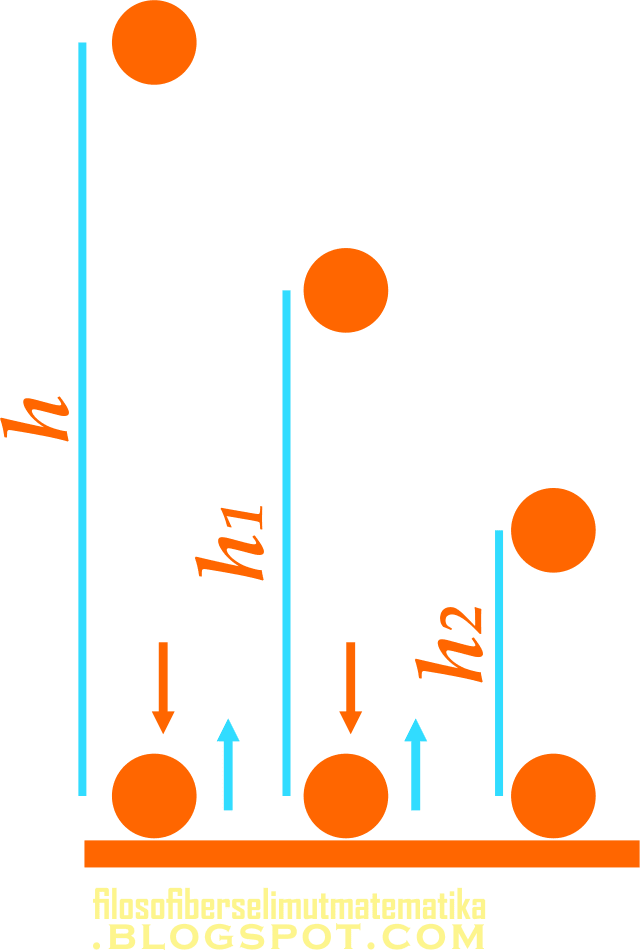
\includegraphics[width=0.3\linewidth]{images/gambar restitusi.png}
    \caption{Diagram skematik tumbukan \textit{bola} dengan permukaan datar menunjukkan komponen kecepatan sebelum dan setelah tumbukan}
    \label{fig:teori-figure-1}
\end{figure}

\begin{equation}
    e = \frac{|v_{r}'|}{|v_{r}|} = \frac{|v_2' - v_1'|}{|v_1 - v_2|}
\end{equation}

dengan:
\begin{itemize}
    \item $e$ = koefisien restitusi (tanpa dimensi)
    \item $v_{r}'$ = kecepatan relatif sesudah tumbukan (m/s)
    \item $v_{r}$ = kecepatan relatif sebelum tumbukan (m/s)
    \item $v_1', v_2'$ = kecepatan benda 1 dan 2 sesudah tumbukan (m/s)
    \item $v_1, v_2$ = kecepatan benda 1 dan 2 sebelum tumbukan (m/s)
\end{itemize}

Untuk kasus khusus tumbukan vertikal dengan permukaan datar, perhitungan koefisien restitusi dapat disederhanakan. Dalam hal ini, analisis menjadi lebih mudah karena dapat menggunakan hubungan antara ketinggian awal dan ketinggian pantulan:

\begin{equation}
    e = \sqrt{\frac{h_2}{h_1}}
\end{equation}

dengan:
\begin{itemize}
    \item $h_1$ = tinggi awal pelepasan benda (m)
    \item $h_2$ = tinggi pantulan maksimum sesudah tumbukan (m)
\end{itemize}

\subsection{Klasifikasi Tumbukan Berdasarkan Nilai Koefisien Restitusi}
Berdasarkan nilai koefisien restitusi yang diperoleh, tumbukan dapat dikelompokkan menjadi tiga kategori utama. Setiap kategori mencerminkan karakteristik energi yang berbeda-beda.

Tumbukan \textit{elastis sempurna} terjadi apabila nilai koefisien restitusi sama dengan satu ($e = 1$). Pada kondisi ini, seluruh energi kinetik sistem tetap terjaga. Fenomena semacam ini biasanya dijumpai pada tumbukan antar\textit{partikel} dalam kondisi ideal \citep{stronge2018impact}. 

Kondisi berikutnya adalah tumbukan \textit{tidak elastis sempurna} yang memiliki nilai koefisien restitusi nol ($e = 0$). Dalam keadaan ini, seluruh energi kinetik relatif berubah menjadi energi internal seperti panas dan deformasi permanen \citep{johnson1987contact}. 

Kategori terakhir merupakan tumbukan \textit{tidak elastis sebagian} dengan rentang nilai antara nol dan satu ($0 < e < 1$). Pada kondisi ini, sebagian energi kinetik hilang dalam proses tumbukan. Kondisi seperti ini merupakan fenomena yang umum dijumpai dalam tumbukan nyata \citep{cross2002coefficient}.

\subsection{Hubungan Koefisien Restitusi dengan Sifat Material dan Deformasi}
Nilai koefisien restitusi sangat bergantung pada karakteristik intrinsik material. Karakteristik tersebut meliputi \textit{modulus elastisitas} ($E$), \textit{batas luluh} (\(\sigma_y\)), dan sifat \textit{viskoelastik} material \citep{meyer2020coefficient}. 

Material yang memiliki \textit{modulus elastisitas} tinggi seperti baja atau keramik umumnya menunjukkan nilai $e$ yang lebih besar. Hal ini berbeda dengan material yang memiliki \textit{modulus} rendah seperti polimer atau busa \citep{brancazio1981physics}. 

Proses deformasi selama tumbukan berlangsung dapat dibagi menjadi dua fase yang saling berkaitan, yaitu \textit{kompresi} dan \textit{restorasi}. Pada fase \textit{kompresi}, energi kinetik diubah menjadi energi deformasi elastis dan plastis. Sementara itu, pada fase \textit{restorasi}, energi deformasi elastis dikembalikan menjadi energi kinetik. Adapun energi deformasi plastis menjadi energi disipasi \citep{hartono2019analisis}.

\subsection{Faktor-Faktor yang Memengaruhi Koefisien Restitusi}

Beberapa faktor memengaruhi nilai koefisien restitusi dalam proses tumbukan nyata. \textit{Kecepatan tumbukan} merupakan faktor pertama yang cukup signifikan. Peningkatan \textit{kecepatan tumbukan} menyebabkan deformasi plastis yang lebih besar sehingga menurunkan nilai $e$ \citep{smith2018experimental}. 

Karakteristik permukaan juga berperan penting dalam menentukan nilai koefisien restitusi. \textit{Kekasaran permukaan} ($R_a$) dan kondisi pelumasan memengaruhi energi disipasi melalui gesekan \citep{penner2002physics}. 

\textit{Temperatur lingkungan} memberikan pengaruh terhadap sifat material. Peningkatan \textit{temperatur} menurunkan \textit{modulus elastisitas} material yang berdampak pada penurunan nilai $e$ \citep{lamb1945hydrodynamics}. 

\textit{Geometri benda} turut memengaruhi distribusi tegangan selama tumbukan berlangsung. Bentuk dan ukuran relatif benda menentukan pola deformasi yang terjadi \citep{stronge2018impact}.

\section{Sensor Ultrasonik HC-SR04}

\subsection{Prinsip Kerja dan Teori Dasar}
Sensor ultrasonik HC-SR04 bekerja berdasarkan prinsip \textit{time-of-flight} (TOF) dengan menggunakan gelombang ultrasonik berfrekuensi 40 kHz \citep{fauzi2020pengujian}. Prinsip kerja sensor ini mengikuti persamaan dasar yang menghubungkan jarak dengan waktu tempuh gelombang:

\begin{equation}
    d = \frac{v \cdot t}{2}
\end{equation}

dengan:
\begin{itemize}
    \item $d$ = jarak objek dari sensor (m)
    \item $v$ = kecepatan suara dalam udara (m/s)
    \item $t$ = waktu tempuh gelombang ultrasonik (s)
    \item Faktor 2 dalam penyebut disebabkan oleh perjalanan gelombang \textit{bolak-balik}
\end{itemize}

Kecepatan suara dalam udara dapat dihitung dengan menggunakan persamaan yang mempertimbangkan pengaruh \textit{temperatur lingkungan}:

\begin{equation}
    v = 331,4 + 0,6 \cdot T
\end{equation}

dengan:
\begin{itemize}
    \item $T$ = \textit{temperatur udara} dalam Celsius (°C)
    \item 331,4 = kecepatan suara pada 0°C (m/s)
    \item 0,6 = \textit{koefisien temperatur} (m/s·°C)
\end{itemize}

\subsection{Spesifikasi Teknis}
Sensor HC-SR04 memiliki karakteristik teknis yang mendukung aplikasi pengukuran jarak dengan presisi tinggi \citep{siregar2021sensor}. Sensor ini beroperasi pada tegangan 5V DC dengan konsumsi arus sebesar 15 mA. Rentang pengukurannya mencapai 2 cm hingga 400 cm dengan akurasi ±3 mm. 

Sudut deteksi sensor mencapai 15° yang memungkinkan deteksi objek dalam area yang cukup luas. Sensor menggunakan frekuensi ultrasonik 40 kHz untuk transmisi gelombang. Untuk mengaktifkan proses pengukuran, sensor memerlukan durasi pulsa \textit{trigger} minimum 10 $\mu$s.

\subsection{Konfigurasi Pin dan Antarmuka}
Sensor HC-SR04 dirancang dengan empat pin utama. Setiap pin memiliki fungsi spesifik dalam sistem pengukuran. Pin VCC berfungsi sebagai input tegangan 5V DC untuk suplai daya sensor. Pin GND merupakan \textit{ground} atau referensi tegangan 0V. Pin \textit{Trig} adalah input untuk memicu pengiriman gelombang ultrasonik. Pin \textit{ECHO} adalah output yang memberikan pulsa dengan lebar yang sebanding dengan jarak objek yang dideteksi. 

Konfigurasi pin ini ditunjukkan pada Gambar \ref{fig:teori-figure-2} yang menggambarkan diagram pin dan konfigurasi sensor ultrasonik HC-SR04.

\begin{figure}
    \centering
    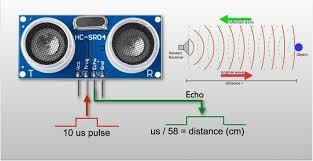
\includegraphics[width=0.5\linewidth]{images/hcsr.jpg}
    \caption{Diagram pin dan konfigurasi sensor ultrasonik HC-SR04}
    \label{fig:teori-figure-2}
\end{figure}

\subsection{Algoritma Pengukuran}
Proses pengukuran jarak menggunakan sensor HC-SR04 mengikuti algoritma yang terstruktur dan dapat diandalkan \citep{rohman2021aplikasi}. Proses dimulai dengan memberikan pulsa HIGH selama 10 $\mu$s pada pin \textit{Trigger} untuk mengaktifkan transmisi gelombang ultrasonik. 

Selanjutnya, pin \textit{ECHO} akan berubah menjadi HIGH ketika gelombang ultrasonik dipancarkan. Pin ini kembali menjadi LOW ketika gelombang pantul diterima oleh sensor. Sistem kemudian mengukur durasi pulsa HIGH pada pin \textit{ECHO} dan menghitung jarak menggunakan persamaan TOF yang telah ditetapkan. Algoritma ini memastikan pengukuran yang konsisten dan akurat dalam berbagai kondisi operasional.

\section{Mikrokontroler ESP8266}

\subsection{Arsitektur dan Spesifikasi}
ESP8266 adalah \textit{System-on-Chip} (SoC) yang mengintegrasikan mikrokontroler 32-bit berbasis arsitektur \textit{Tensilica L106} dengan modul \textit{Wi-Fi IEEE 802.11 b/g/n} \citep{rodrigues2018vision}. Sistem ini menggunakan prosesor \textit{Tensilica L106 32-bit RISC} dengan \textit{clock} hingga 160 MHz yang memberikan performa komputasi yang memadai untuk aplikasi \textit{IoT}. 

Konfigurasi memori meliputi 64 KB RAM instruksi dan 96 KB RAM data untuk operasi waktu nyata. Sistem dilengkapi \textit{flash} eksternal berkapasitas 512 KB hingga 4 MB untuk penyimpanan program dan data. 

Sistem dilengkapi dengan 16 pin digital I/O yang dapat dikonfigurasi sesuai kebutuhan aplikasi. Terdapat satu kanal \textit{ADC 10-bit} dengan rentang 0-1V untuk pembacaan sensor analog. \textit{Interface komunikasi} yang tersedia meliputi \textit{UART}, \textit{SPI}, dan \textit{I2C}. Mikrokontroler beroperasi pada tegangan 3,3V dengan konsumsi daya 80 mA dalam mode aktif dan 20 $\mu$A dalam mode \textit{deep sleep} untuk efisiensi energi.

\begin{figure}
    \centering
    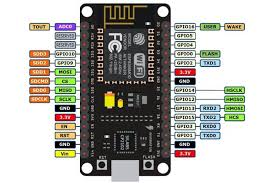
\includegraphics[width=0.5\linewidth]{images/esp 8266.jpg}
    \caption{Modul ESP8266 dengan konfigurasi pin GPIO}
    \label{fig:teori-figure-3}
\end{figure}

\subsection{Konfigurasi Pin dan Fungsionalitas}
Konfigurasi pin ESP8266 dirancang untuk fleksibilitas maksimum dalam berbagai aplikasi \textit{IoT}. Pin GPIO0 hingga GPIO16 berfungsi sebagai I/O digital dengan kemampuan \textit{PWM} dan \textit{interrupt}. Hal ini memungkinkan \textit{interfacing} dengan berbagai sensor dan aktuator. 

Pin \textit{ADC} khusus disediakan untuk pembacaan sensor analog yang memerlukan konversi sinyal analog ke digital. Pin \textit{TX/RX} digunakan untuk komunikasi \textit{UART} yang memfasilitasi \textit{serial debugging} dan komunikasi dengan perangkat eksternal. 

Pin \textit{RST} berfungsi sebagai \textit{reset} untuk \textit{restart} sistem dalam kondisi tertentu. Adapun pin \textit{EN} merupakan \textit{enable pin} untuk aktivasi chip secara keseluruhan. Gambar \ref{fig:teori-figure-3} menunjukkan modul ESP8266 dengan konfigurasi pin GPIO yang lengkap.

\subsection{Pemrograman dan Development Environment}
ESP8266 mendukung berbagai lingkungan pengembangan yang memfasilitasi implementasi aplikasi \textit{IoT} dengan fleksibilitas tinggi. \textit{Arduino IDE} dengan \textit{ESP8266 Core} merupakan platform yang paling populer. Platform ini memungkinkan penggunaan sintaks \textit{Arduino} untuk pemrograman yang familiar bagi sebagian besar \textit{developer} \citep{monk2016programming}. 

\textit{Framework} alternatif yang didukung meliputi \textit{ESP-IDF} untuk pengembangan tingkat lanjut, \textit{MicroPython} untuk \textit{rapid prototyping}, dan \textit{NodeMCU Lua} untuk pengembangan berbasis \textit{scripting}. Keberagaman platform ini memungkinkan \textit{developer} memilih lingkungan yang paling sesuai dengan kebutuhan proyek dan tingkat kompleksitas aplikasi.

\section{\textit{Internet of Things} (IoT)}

\subsection{Definisi dan Konsep Fundamental}
\textit{Internet of Things} (IoT) adalah paradigma komputasi yang memungkinkan objek fisik (\textit{things}) terhubung ke \textit{internet} dan saling berkomunikasi untuk bertukar data secara otomatis tanpa intervensi manusia \citep{ashton2009internet}. Konsep ini melibatkan integrasi sensor, aktuator, komunikasi nirkabel, dan sistem komputasi \textit{awan} untuk menciptakan ekosistem digital yang cerdas \citep{ray2018survey}. 

Implementasi \textit{IoT} memungkinkan pengumpulan data waktu nyata dari lingkungan fisik. Selain itu, \textit{IoT} juga memungkinkan pemrosesan data menggunakan algoritma cerdas dan respons otomatis terhadap kondisi tertentu.

\subsection{Arsitektur IoT}
Arsitektur \textit{IoT} umumnya terdiri atas empat lapisan utama yang saling terintegrasi untuk menciptakan sistem yang komprehensif \citep{weber2010governance}. 

Lapisan \textit{persepsi} merupakan fondasi sistem yang terdiri atas sensor dan aktuator. Lapisan ini mengumpulkan data lingkungan dan melakukan aksi berdasarkan instruksi yang diterima. 

Lapisan \textit{jaringan} menangani transmisi data melalui berbagai protokol komunikasi seperti \textit{Wi-Fi}, \textit{Bluetooth}, \textit{ZigBee}, atau \textit{LoRaWAN} sesuai dengan kebutuhan aplikasi. 

Lapisan \textit{pemrosesan} melakukan analisis dan pemrosesan data menggunakan algoritma yang sesuai, baik secara lokal maupun di \textit{cloud computing}. 

Lapisan \textit{aplikasi} menyediakan antarmuka pengguna dan layanan aplikasi yang memungkinkan interaksi antara pengguna dengan sistem \textit{IoT}.

\subsection{Protokol Komunikasi IoT}
Sistem \textit{IoT} menggunakan berbagai protokol komunikasi yang dipilih berdasarkan kebutuhan spesifik aplikasi. Pemilihan protokol didasarkan pada jangkauan, konsumsi daya, dan \textit{throughput} data. 

\textit{Wi-Fi IEEE 802.11} digunakan untuk komunikasi lokal berkecepatan tinggi dengan konsumsi daya yang relatif tinggi namun memberikan \textit{bandwidth} yang luas. 

\textit{Bluetooth} dan \textit{Bluetooth Low Energy} (BLE) cocok untuk komunikasi jarak pendek dengan konsumsi daya rendah. Protokol ini ideal untuk aplikasi \textit{wearable} dan sensor personal. 

\textit{ZigBee} berdasarkan \textit{IEEE 802.15.4} dirancang khusus untuk jaringan sensor nirkabel dengan topologi \textit{mesh} yang dapat mengcover area yang luas. 

\textit{LoRaWAN} (\textit{Long Range Wide Area Network}) dikembangkan untuk komunikasi jarak jauh dengan daya rendah. Protokol ini sangat sesuai untuk aplikasi \textit{smart city} dan \textit{monitoring lingkungan}.

\subsection{Message Queuing Telemetry Transport (MQTT)}
\textit{MQTT} adalah protokol komunikasi \textit{publish-subscribe} yang dirancang khusus untuk aplikasi \textit{IoT} dengan \textit{bandwidth} terbatas dan koneksi tidak stabil \citep{zhang2021iot}. Protokol ini beroperasi di atas \textit{TCP/IP} dan menggunakan arsitektur \textit{broker-client} yang memungkinkan komunikasi yang efisien dan dapat diandalkan. 

Desain \textit{MQTT} memprioritaskan efisiensi \textit{bandwidth} dan ketahanan terhadap gangguan jaringan. Hal ini menjadikannya ideal untuk aplikasi \textit{IoT} yang memerlukan transmisi data waktu nyata dengan konsumsi daya minimal.

\subsubsection{Arsitektur MQTT}
Sistem \textit{MQTT} terdiri atas tiga komponen utama yang bekerja secara sinergis. \textit{Publisher} merupakan perangkat yang mengirim data ke \textit{broker} dengan \textit{topik} tertentu yang telah ditentukan. 

\textit{Broker} berfungsi sebagai \textit{server} yang menerima, memfilter, dan mendistribusikan pesan kepada \textit{subscriber} yang berlangganan \textit{topik} tertentu. 

\textit{Subscriber} adalah perangkat yang menerima data dari \textit{broker} berdasarkan \textit{topik} yang telah mereka \textit{subscribe} sebelumnya. Arsitektur ini memungkinkan komunikasi \textit{many-to-many} yang efisien dan fleksibel.

\subsubsection{Quality of Service (QoS) dalam MQTT}
\textit{MQTT} mendefinisikan tiga level \textit{Quality of Service} (QoS) untuk pengiriman pesan. Hal ini memberikan fleksibilitas dalam menentukan tingkat keandalan transmisi data \citep{anderson2019digital}. 

QoS 0 atau \textit{At most once} memungkinkan pesan dikirim maksimal satu kali tanpa konfirmasi. Tingkat ini cocok untuk data yang tidak kritis dan dapat mentolerir kehilangan data. 

QoS 1 atau \textit{At least once} menjamin pesan terkirim minimal satu kali dengan kemungkinan duplikasi. Tingkat ini sesuai untuk data penting yang memerlukan konfirmasi penerimaan. 

QoS 2 atau \textit{Exactly once} menjamin pesan terkirim tepat satu kali tanpa duplikasi. Tingkat ini ideal untuk data kritis yang memerlukan integritas tinggi.

\subsubsection{Struktur Topik MQTT}
\textit{Topik MQTT} menggunakan struktur hierarkis dengan separator "/" 
untuk mengorganisir data secara sistematis dan logis. Contoh implementasi 
dalam penelitian ini menggunakan struktur seperti berikut
\begin{verbatim}
sensor/koefisien_restitusi/bola_tenis/tinggi_awal
sensor/koefisien_restitusi/bola_tenis/tinggi_pantul
\end{verbatim}
Struktur ini memungkinkan kategorisasi data berdasarkan jenis sensor, parameter yang 
diukur, objek pengukuran, dan jenis data spesifik.



\section{Karakteristik Material Bola}

\subsection{Klasifikasi Material Berdasarkan Sifat Mekanik}
Material bola dapat diklasifikasikan berdasarkan sifat mekaniknya yang memengaruhi koefisien restitusi secara signifikan \citep{kalnins2018separation}. 

Material \textit{elastis} seperti polimer dengan \textit{modulus elastisitas} tinggi menunjukkan kemampuan pemulihan bentuk yang baik setelah deformasi. Hal ini menghasilkan koefisien restitusi yang relatif tinggi. 

Material \textit{viskoelastis} termasuk karet alam dan sintetis memiliki karakteristik yang menggabungkan sifat elastis dan viskos. Pada material ini, respons terhadap beban bergantung pada waktu dan kecepatan pembebanan. 

Material \textit{komposit} yang merupakan kombinasi serat dan matriks polimer menunjukkan sifat mekanik yang dapat disesuaikan. Penyesuaian dilakukan berdasarkan orientasi serat dan jenis matriks yang digunakan.

\subsection{Hubungan Modulus Elastisitas dengan Koefisien Restitusi}
\textit{Modulus elastisitas} ($E$) material didefinisikan sebagai perbandingan antara \textit{tegangan normal} ($\sigma$) terhadap \textit{regangan normal} ($\varepsilon$). Nilai ini memberikan ukuran kekakuan material:

\begin{equation}
    E = \frac{\sigma}{\varepsilon}
\end{equation}

dengan:
\begin{itemize}
    \item $E$ = \textit{modulus elastisitas} (Pa)
    \item $\sigma$ = \textit{tegangan normal} (Pa)
    \item $\varepsilon$ = \textit{regangan normal} (tanpa dimensi)
\end{itemize}

\textit{Tegangan} dan \textit{regangan} dapat dihitung menggunakan persamaan yang menghubungkan gaya dan deformasi dengan sifat geometris material:

\begin{equation}
    \sigma = \frac{F}{A}
\end{equation}

\begin{equation}
    \varepsilon = \frac{\Delta L}{L_0}
\end{equation}

dengan:
\begin{itemize}
    \item $F$ = gaya yang diterapkan (N)
    \item $A$ = luas penampang ($m^2$)
    \item $\Delta L$ = perubahan panjang (m)
    \item $L_0$ = panjang awal (m)
\end{itemize}

\subsection{Geometri Bola dan Kalkulasi Volume}
\textit{Geometri bola} memainkan peran penting dalam analisis karakteristik material dan perhitungan parameter fisik. \textit{Volume bola} ($V$) dihitung menggunakan persamaan geometris fundamental:

\begin{equation}
    V = \frac{4}{3}\pi r^3
\end{equation}

dengan:
\begin{itemize}
    \item $V$ = \textit{volume bola} (m³)
    \item $r$ = \textit{jari-jari bola} (m)
    \item $\pi$ = konstanta pi (3,14159...)
\end{itemize}

\textit{Luas permukaan bola} ($A$) diberikan oleh persamaan yang menentukan area kontak potensial selama tumbukan:

\begin{equation}
    A = 4\pi r^2
\end{equation}

dengan:
\begin{itemize}
    \item $A$ = \textit{luas permukaan bola} ($m^2$)
\end{itemize}

\subsection{Material Bola dalam Penelitian}
Penelitian ini menggunakan lima jenis bola dengan karakteristik material yang berbeda. Hal ini bertujuan memberikan variasi yang komprehensif dalam analisis koefisien restitusi \citep{avancini2020physical}. 

\textit{Bola tenis meja} terbuat dari \textit{selulosa asetat} dengan densitas rendah yang memberikan karakteristik pantulan yang responsif dan konsisten. 

\textit{Bola bekel} menggunakan \textit{karet sintetis} dengan elastisitas tinggi yang memungkinkan pemulihan energi yang efisien selama proses tumbukan. 

\textit{Bola plastik} terbuat dari \textit{polietilena} dengan sifat termoplastik yang menunjukkan deformasi plastis yang signifikan selama tumbukan. 

\textit{Bola karet} menggunakan \textit{karet alam} dengan sifat viskoelastis yang memberikan respons yang bergantung pada kecepatan deformasi. 

\textit{Bola baseball} menggunakan material \textit{komposit berlapis} yang menggabungkan berbagai material untuk mengoptimalkan performa dan durabilitas. 

Setiap material memiliki karakteristik unik yang memengaruhi respons dinamis selama proses tumbukan. Hal ini tercermin dalam nilai koefisien restitusi yang berbeda untuk setiap jenis bola dan memberikan wawasan mendalam tentang hubungan antara sifat material dan perilaku tumbukan.
\chapter{METODE PENELITIAN}\label{cha:metode}


\section{Waktu dan Tempat Pelaksanaan Penelitian}
\paragraph{}Penelitian ini direncanakan untuk dilaksanakan secara intensif selama bulan Februari, memanfaatkan momentum awal tahun untuk mencapai hasil yang optimal. Lokasi penelitian berada di \textbf{Jalan Desa Cipadung, Gang Bho Optikal, RT 03 RW 04, Kosan Armani Nomor 104}. Lokasi ini dapat dengan mudah ditemukan karena terdapat pos ronda di area Gang Bho, wilayah Cibiru, Kota Bandung, Jawa Barat, dengan kode pos 40614.

\paragraph{}Keunikan penelitian ini terletak pada penggunaan alat yang dirancang secara khusus dengan tingkat presisi tinggi untuk mendukung seluruh tahap eksperimen. Dengan lokasi strategis dan penggunaan alat inovatif, penelitian ini diharapkan dapat memberikan kontribusi yang signifikan.

\begin{figure}
    \centering
    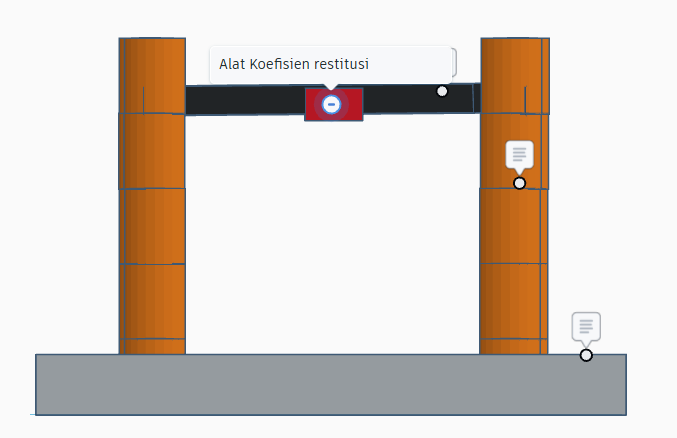
\includegraphics[width = 18pc]{images/Ilustrasi Alat.png}
    \caption{Ilustrasi Alat}
    \label{fig:ilustrasi_alat}
\end{figure}
\paragraph{}Skema berikut menunjukkan alat yang dilengkapi dengan tiang penyangga dan tiang penopang pada box alat penelitian, yang dirancang untuk mencegah goncangan dan memastikan kestabilan selama proses pengambilan data.
\begin{figure}
    \centering
    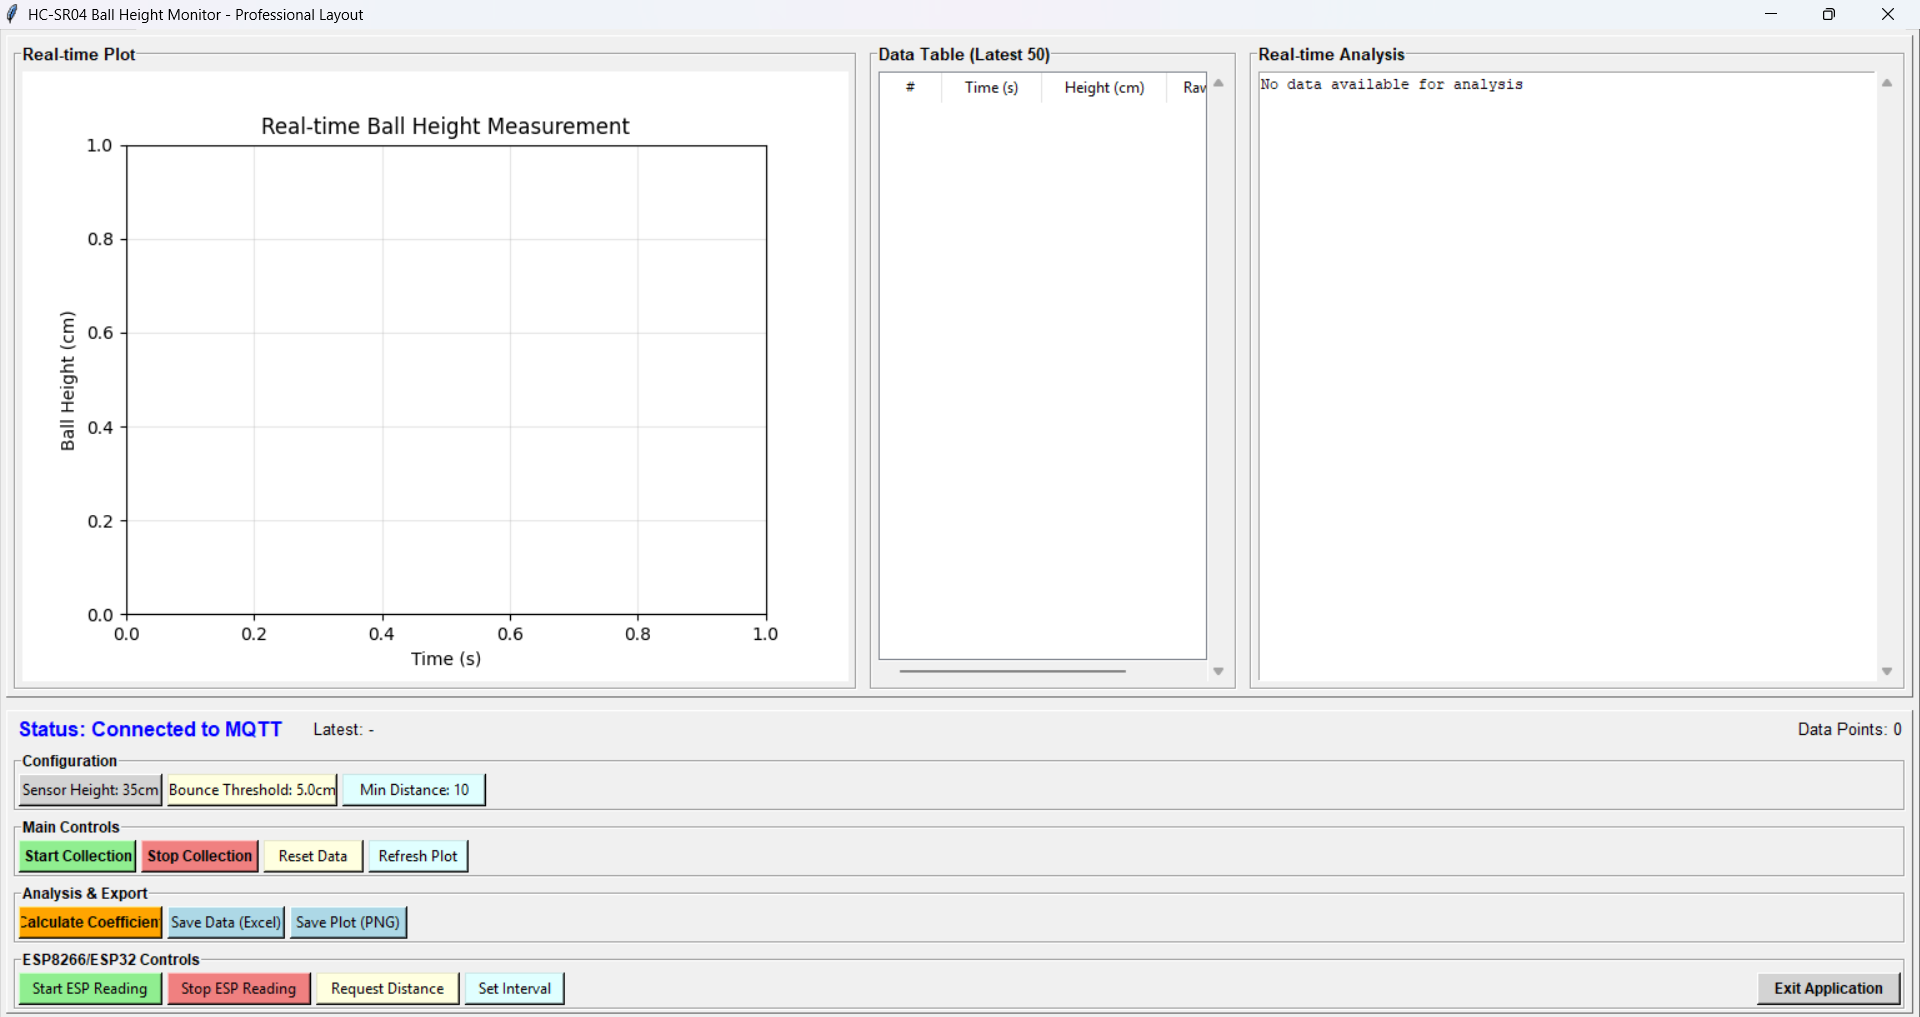
\includegraphics[width =\textwidth]{images/Tampilan GUI.png}
    \caption{Tampilan GUI}
    \label{fig:tampilan_gui}
\end{figure}
\paragraph{}Desain antarmuka pengguna aplikasi Python ini menerapkan prinsip Human-Computer Interaction (HCI) modern dengan mengintegrasikan teknologi Internet of Things (IoT) berbasis protokol Message Queuing Telemetry Transport (MQTT) untuk monitoring koefisien restitusi secara real-time. Implementasi graphical user interface (GUI) menggunakan framework Tkinter menyediakan dashboard interaktif yang memungkinkan operator melakukan kontrol sistem sensor, visualisasi data time-series, dan analisis statistik dengan tingkat responsivitas tinggi. Arsitektur client-server ini memanfaatkan cloud broker HiveMQ sebagai middleware komunikasi yang menjamin delivery reliability dan scalability sistem monitoring jarak jauh.

\paragraph{}Interface aplikasi dirancang dengan modular architecture yang terdiri dari control panel untuk command transmission, real-time plotting module untuk visualization data trajectory bola, dan analysis dashboard untuk statistical computation koefisien restitusi. Setiap komponen GUI terintegrasi dengan event-driven programming model yang memastikan seamless interaction antara user input dan system response. Protokol MQTT Quality of Service (QoS) level 1 diimplementasikan untuk guaranteed message delivery antara aplikasi Python dan embedded device ESP8266, sedangkan JSON serialization digunakan untuk structured data exchange yang mempertahankan data integrity dan parsing efficiency.
\begin{figure}
    \centering
    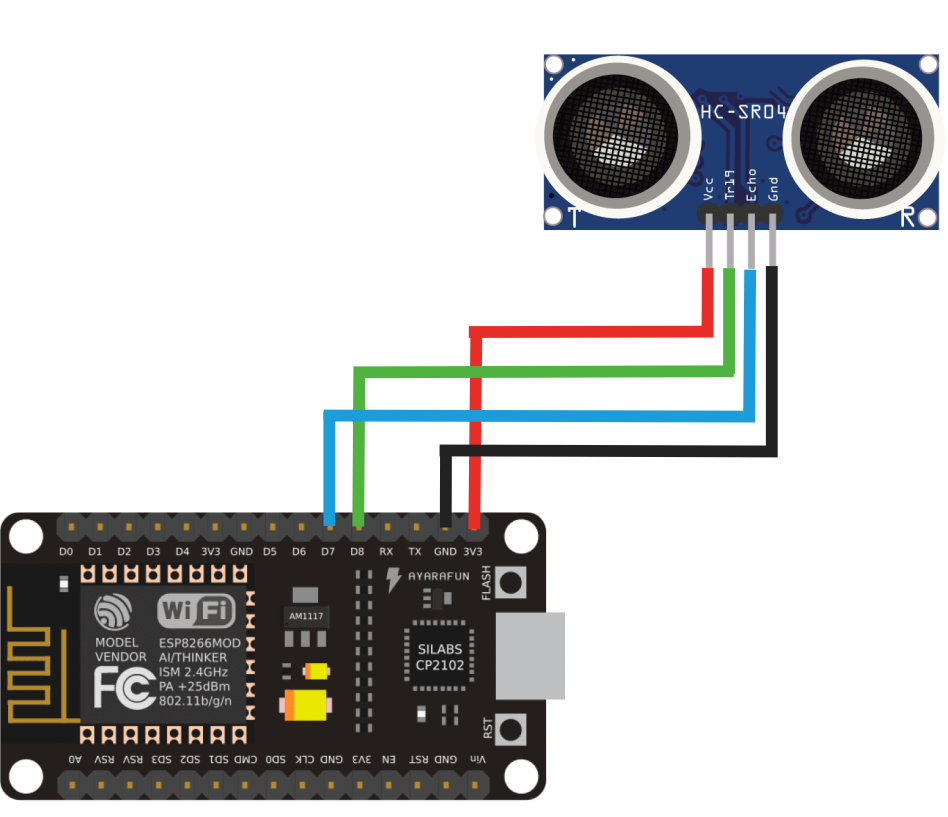
\includegraphics[width=0.5\linewidth]{images/Skematik Rangkaian.png}
    \caption{skematik rangkaian}
    \label{fig:skematik_rangkaian}
\end{figure}
\paragraph{}Ini adalah skematik rangkaian yang menunjukkan cara menghubungkan sensor HCSR-04 dengan modul ESP8266. Pada rangkaian ini, VCC dari HCSR-04 disambungkan ke pin 3V pada ESP8266, sedangkan GND HCSR-04 dihubungkan ke GND ESP8266. Untuk pin TRIG, HCSR-04 dapat disambungkan ke pin mana saja pada ESP8266, namun dalam contoh ini digunakan pin D8. Begitu juga dengan pin ECHO, yang disambungkan ke pin D7, meskipun dapat disesuaikan dengan pin lain sesuai kebutuhan.
\paragraph{}Eksperimen dilakukan sebanyak 100 kali dengan menggunakan lima jenis bola yang berbeda. Setiap jenis bola diuji sebanyak 20 kali.

\section{Alat dan Bahan Penelitian}
Alat dan bahan yang digunakan dalam penelitian ini dijelaskan sebagai berikut:

\subsection{Alat Penelitian}
Berikut adalah daftar alat yang digunakan:
\begin{table}[H]
\caption{Tabel Peralatan}
\label{tab:alat}
\begin{center}
    \begin{tabular}{|l|l|l|}
    \hline
        \textbf{No} & \textbf{Alat Penelitian} & \textbf{Jumlah Alat} \\\hline
        1 & Laptop & 1 buah \\\hline
        2 & ESP8266 & 1 buah \\\hline
        3 & HCSR-04 & 1 buah \\\hline
        4 & Kabel Jumper & Secukupnya \\\hline
        5 & Akrilik & Secukupnya \\\hline
        6 & Pipa Besi & Secukupnya \\\hline
        7 & Mur dan Baut & Secukupnya \\\hline
        8 & Penyambung Pipa & Secukupnya \\\hline
        9 & \textit{Software} Arduino & - \\\hline
    \end{tabular}
\end{center}
\end{table}

\subsection{Bahan Penelitian}
Berikut adalah daftar bahan yang digunakan:
\begin{table}[H]
\caption{Tabel Bahan}
\label{tab:bahan}
\begin{center}
    \begin{tabular}{|l|l|l|}
    \hline
        \textbf{No} & \textbf{Bahan Penelitian} & \textbf{Jumlah Bahan} \\\hline
        1 & Bola Tenis Meja & 1 buah \\\hline
        2 & Bola Bekel & 1 buah \\\hline
        3 & Bola Sepak Karet & 1 buah \\\hline
        4 & Bola Plastik & 1 buah \\\hline
        5 & Bola Tenis lapang & 1 buah \\\hline
    \end{tabular}
\end{center}
\end{table}

\section{Diagram Alir Penelitian}
\subsection{Flowchart Program Python}

\begin{figure}[H]
\centering
\begin{tikzpicture} [
    node distance=0.5cm,
    start/.style={ellipse, draw=black, thick, fill=green!30, minimum width=2.5cm, minimum height=1cm, font=\tiny, text centered},
    process/.style={rectangle, draw=black, thick, fill=blue!30, minimum width=2.5cm, minimum height=1cm, font=\tiny, text centered},
    decision/.style={diamond, draw=black, thick, fill=yellow!30, minimum width=2cm, minimum height=2cm, font=\tiny, text centered, inner sep=1pt},
    terminal/.style={ellipse, draw=black, thick, fill=red!30, minimum width=2cm, minimum height=1cm, font=\tiny, text centered},
    arrow/.style={->, thick, >=stealth}
]

% Layer 1: Define all nodes first (foreground)
\node[start] (start) {Mulai\\Aplikasi Python};
\node[process, below=of start] (init) {Inisialisasi GUI\\Setup MQTT\\Koneksi Broker};
\node[process, below=of init] (loop) {Loop Event Utama};
\node[decision, below=of loop, xshift=-3cm] (mqtt_msg) {Pesan\\MQTT?};
\node[decision, below=of loop, xshift=3cm] (user_action) {Aksi\\Pengguna?};
\node[process, below=of mqtt_msg] (parse) {Parse JSON\\Validasi Data};
\node[decision, below=of parse] (collecting) {Mengumpulkan\\Data?};
\node[process, below=of collecting] (store) {Simpan Data\\Update Plot};
\node[process, below=of user_action] (handle) {Tangani Input\\Pengguna};
\node[decision, below=of handle] (analyze) {Hitung\\Koefisien?};
\node[process, below=of analyze] (calc) {Deteksi Pantulan\\Hitung e};
\node[process, below=of store, xshift=3cm] (update) {Update GUI\\Tampilkan Hasil};
\node[terminal, below=of update] (end) {Keluar\\Aplikasi};

% Layer 2: Draw all arrows in background
\begin{scope}[on background layer]
    % Main Flow Arrows
    \draw[arrow, blue!70, line width=1.2pt] (start) -- (init);
    \draw[arrow, blue!70, line width=1.2pt] (init) -- (loop);
    
    % Branch to decisions
    \draw[arrow, blue!70, line width=1.2pt] (loop) -- (mqtt_msg);
    \draw[arrow, blue!70, line width=1.2pt] (loop) -- (user_action);
    
    % MQTT Branch
    \draw[arrow, green!70, line width=1.2pt] (mqtt_msg) -- node[right, fill=white, inner sep=1pt, font=\tiny] {Ya} (parse);
    \draw[arrow, green!70, line width=1.2pt] (parse) -- (collecting);
    \draw[arrow, green!70, line width=1.2pt] (collecting) -- node[right, fill=white, inner sep=1pt, font=\tiny] {Ya} (store);
    \draw[arrow, green!70, line width=1.2pt] (store) -- (update);
    
    % User Branch
    \draw[arrow, purple!70, line width=1.2pt] (user_action) -- node[left, fill=white, inner sep=1pt, font=\tiny] {Ya} (handle);
    \draw[arrow, purple!70, line width=1.2pt] (handle) -- (analyze);
    \draw[arrow, purple!70, line width=1.2pt] (analyze) -- node[right, fill=white, inner sep=1pt, font=\tiny] {Ya} (calc);
    \draw[arrow, purple!70, line width=1.2pt] (calc) -- (update);
    
    % No Branches to Update
    \draw[arrow, red!60, line width=1pt] (mqtt_msg) -- node[above, fill=white, inner sep=1pt, font=\tiny] {Tidak} ++(3,0) |- (update);
    \draw[arrow, red!60, line width=1pt] (user_action) -- node[above, fill=white, inner sep=1pt, font=\tiny] {Tidak} ++(-3,0) |- (update);
    \draw[arrow, red!60, line width=1pt] (collecting) -- node[left, fill=white, inner sep=1pt, font=\tiny] {Tidak} ++(-1.5,0) |- (update);
    \draw[arrow, red!60, line width=1pt] (analyze) -- node[left, fill=white, inner sep=1pt, font=\tiny] {Tidak} ++(-1.5,0) |- (update);
    
    % Loop Back
    \draw[arrow, orange!60, line width=1pt, dashed] (update) -- ++(4,0) |- (loop);
    
    % Exit
    \draw[arrow, gray!70, line width=1.2pt] (update) -- (end);
\end{scope}

\end{tikzpicture}
\caption{Flowchart Program Python}
\end{figure}

\textbf{Penjelasan Program Python:} 

Aplikasi Python ini adalah program utama yang berfungsi sebagai pusat kontrol seluruh sistem monitoring koefisien restitusi bola. Program ini dirancang dengan antarmuka grafis (GUI) yang user-friendly menggunakan library Tkinter sehingga pengguna dapat dengan mudah mengoperasikan sistem tanpa perlu memahami kode programming.

\textbf{Cara Kerja Program Python:}

\paragraph{Inisialisasi Sistem} Saat program dimulai, sistem melakukan setup GUI (tampilan aplikasi), mengatur koneksi MQTT ke cloud broker HiveMQ, dan mempersiapkan semua komponen yang diperlukan untuk monitoring real-time. Proses ini memastikan bahwa semua library yang diperlukan telah dimuat dengan benar dan interface pengguna siap untuk digunakan.

\paragraph{Loop Utama Monitoring} Program masuk ke dalam loop pemantauan kontinyu yang secara bersamaan memantau dua hal: (a) pesan data sensor yang dikirim ESP8266 melalui internet via MQTT, dan (b) interaksi pengguna seperti klik tombol atau pengaturan parameter. Loop ini berjalan secara terus-menerus untuk memastikan responsivitas sistem terhadap input dan data yang masuk.

\paragraph{Penerimaan Data Sensor} Ketika ESP8266 mengirim data jarak dalam format JSON melalui internet, program Python menerima, memvalidasi, dan mengonversi data jarak menjadi tinggi bola dengan rumus: tinggi\_bola = tinggi\_sensor - jarak\_terukur. Validasi data dilakukan untuk memastikan kualitas pengukuran dan menghilangkan noise atau error yang mungkin terjadi.

\paragraph{Penyimpanan dan Visualisasi} Data yang valid disimpan dalam array waktu dan tinggi, kemudian divisualisasikan secara real-time dalam grafik yang terus ter-update untuk memudahkan observasi pergerakan bola. Sistem visualisasi ini memungkinkan operator untuk melihat pola pantulan bola secara langsung dan mendeteksi anomali dalam pengukuran.

\paragraph{Analisis Otomatis} Sistem menggunakan algoritma deteksi puncak untuk mengidentifikasi titik-titik pantulan bola, menghitung koefisien restitusi dengan rumus fisika $e = \sqrt{h_2/h_1}$, dan menghasilkan laporan komprehensif tentang karakteristik elastisitas bola. Analisis ini dilakukan secara otomatis setelah cukup data terkumpul untuk memastikan akurasi hasil perhitungan.

\newpage

\subsection{Flowchart Program ESP8266}

\begin{figure}[H]
\centering
\begin{tikzpicture} [
    node distance=0.5cm,
    start/.style={ellipse, draw=black, thick, fill=green!30, minimum width=2.5cm, minimum height=1cm, font=\tiny, text centered},
    process/.style={rectangle, draw=black, thick, fill=blue!30, minimum width=2.5cm, minimum height=1cm, font=\tiny, text centered},
    decision/.style={diamond, draw=black, thick, fill=yellow!30, minimum width=2cm, minimum height=2cm, font=\tiny, text centered, inner sep=1pt},
    arrow/.style={->, thick, >=stealth}
]

% Layer 1: Define all nodes first (foreground)
\node[start] (start) {Mulai\\ESP8266};
\node[process, below=of start] (init_hw) {Inisialisasi\\Pin \& Serial};
\node[process, below=of init_hw] (wifi) {Koneksi\\WiFi};
\node[process, below=of wifi] (mqtt) {Koneksi MQTT\\Subscribe Topik};
\node[process, below=of mqtt] (main_loop) {Loop Utama};
\node[decision, below=of main_loop, xshift=-3cm] (cmd_check) {Perintah\\Diterima?};
\node[decision, below=of main_loop, xshift=3cm] (read_check) {Mode Baca \&\\Interval?};
\node[process, below=of cmd_check] (parse_cmd) {Parse\\Perintah};
\node[decision, below=of parse_cmd] (cmd_type) {Jenis\\Perintah?};
\node[process, below=of cmd_type, xshift=-2cm] (start_read) {Set Pembacaan\\AKTIF};
\node[process, below=of cmd_type, xshift=2cm] (stop_read) {Set Pembacaan\\NONAKTIF};
\node[process, below=of read_check] (sensor) {Baca\\HC-SR04};
\node[process, below=of sensor] (validate) {Validasi\\Data};
\node[process, below=of validate] (json) {Buat\\JSON};
\node[process, below=of json] (publish) {Publish\\MQTT};

% Layer 2: Draw all arrows in background
\begin{scope}[on background layer]
    % Main Flow
    \draw[arrow, blue!70, line width=1.2pt] (start) -- (init_hw);
    \draw[arrow, blue!70, line width=1.2pt] (init_hw) -- (wifi);
    \draw[arrow, blue!70, line width=1.2pt] (wifi) -- (mqtt);
    \draw[arrow, blue!70, line width=1.2pt] (mqtt) -- (main_loop);
    
    % Branches
    \draw[arrow, blue!70, line width=1.2pt] (main_loop) -- (cmd_check);
    \draw[arrow, blue!70, line width=1.2pt] (main_loop) -- (read_check);
    
    % Command Flow
    \draw[arrow, green!70, line width=1.2pt] (cmd_check) -- node[right, fill=white, inner sep=1pt, font=\tiny] {Ya} (parse_cmd);
    \draw[arrow, green!70, line width=1.2pt] (parse_cmd) -- (cmd_type);
    \draw[arrow, green!70, line width=1.2pt] (cmd_type) -- node[above left, fill=white, inner sep=1pt, font=\tiny] {MULAI} (start_read);
    \draw[arrow, green!70, line width=1.2pt] (cmd_type) -- node[above right, fill=white, inner sep=1pt, font=\tiny] {BERHENTI} (stop_read);
    
    % Sensor Flow
    \draw[arrow, purple!70, line width=1.2pt] (read_check) -- node[left, fill=white, inner sep=1pt, font=\tiny] {Ya} (sensor);
    \draw[arrow, purple!70, line width=1.2pt] (sensor) -- (validate);
    \draw[arrow, purple!70, line width=1.2pt] (validate) -- (json);
    \draw[arrow, purple!70, line width=1.2pt] (json) -- (publish);
    
    % Loop Back
    \draw[arrow, orange!60, line width=1pt, dashed] (start_read) |- ++(0,-1) -| (main_loop);
    \draw[arrow, orange!60, line width=1pt, dashed] (stop_read) |- ++(0,-1) -| (main_loop);
    \draw[arrow, orange!60, line width=1pt, dashed] (publish) |- ++(-6,0) |- (main_loop);
    
    % No Action
    \draw[arrow, red!60, line width=1pt] (cmd_check) -- node[above, fill=white, inner sep=1pt, font=\tiny] {Tidak} ++(3,0) |- (main_loop);
    \draw[arrow, red!60, line width=1pt] (read_check) -- node[above, fill=white, inner sep=1pt, font=\tiny] {Tidak} ++(-3,0) |- (main_loop);
\end{scope}

\end{tikzpicture}
\caption{Flowchart Program ESP8266}
\end{figure}

\textbf{Penjelasan Program ESP8266:}

Program ESP8266 berperan sebagai sensor node cerdas yang bekerja secara autonomous (mandiri) untuk mengukur jarak menggunakan sensor ultrasonik HC-SR04 dan mengirimkan data ke aplikasi Python melalui komunikasi internet menggunakan protokol MQTT.

\textbf{Cara Kerja Program ESP8266:}

\paragraph{Inisialisasi Hardware} Saat ESP8266 dinyalakan, program melakukan setup pin GPIO untuk sensor HC-SR04 (pin trigger dan echo), mengatur komunikasi serial untuk debugging, dan menginisialisasi LED built-in sebagai indikator status. Proses ini memastikan bahwa semua komponen hardware siap digunakan dengan konfigurasi yang benar.

\paragraph{Koneksi WiFi} ESP8266 terhubung ke jaringan WiFi menggunakan SSID dan password yang telah dikonfigurasi, memungkinkan akses internet untuk komunikasi dengan broker MQTT cloud. Sistem akan mencoba koneksi berulang kali jika gagal terhubung pada percobaan pertama hingga berhasil mendapatkan koneksi yang stabil.

\paragraph{Setup MQTT} Setelah WiFi terhubung, ESP8266 melakukan koneksi ke broker MQTT di cloud (HiveMQ), subscribe ke topik command untuk menerima perintah dari Python, dan siap mempublikasikan data sensor. Konfigurasi ini memungkinkan komunikasi dua arah antara ESP8266 dan aplikasi Python melalui internet.

\paragraph{Loop Pemrosesan Command} Dalam loop utama, ESP8266 memantau perintah dari aplikasi Python seperti START\_READING (mulai pembacaan kontinyu), STOP\_READING (hentikan pembacaan), atau INTERVAL:nilai (ubah frekuensi pembacaan). Setiap perintah diproses dengan cepat untuk memastikan responsivitas sistem terhadap kontrol pengguna.

\paragraph{Pembacaan Sensor} Ketika mode pembacaan aktif, ESP8266 melakukan pengukuran jarak menggunakan HC-SR04 dengan mengirim gelombang ultrasonik dan menghitung waktu tempuh, kemudian mengkonversi ke jarak dalam satuan centimeter. Pembacaan dilakukan sesuai dengan interval yang telah ditentukan untuk menghasilkan data yang konsisten.

\paragraph{Validasi dan Pengiriman Data} Setiap hasil pembacaan divalidasi (rentang 2-400cm), dikemas dalam format JSON dengan timestamp yang direset setiap START\_READING, dan dikirim ke aplikasi Python melalui topik MQTT. Validasi ini penting untuk memastikan kualitas data dan menghindari pengiriman data yang tidak akurat atau error.

\newpage

\subsection{Komunikasi Sistem}

\textbf{Komunikasi Sistem IoT:}

Sistem ini mengimplementasikan arsitektur Internet of Things (IoT) modern berbasis protokol MQTT yang memungkinkan komunikasi real-time antara perangkat sensor (ESP8266) dan aplikasi monitoring (Python) melalui internet menggunakan cloud broker HiveMQ yang tersedia 24/7.

\textbf{Penjelasan Detail Alur Komunikasi:}

\begin{enumerate}
\item \textbf{Pengiriman Command (Python → MQTT Broker):} Aplikasi Python mengirimkan perintah kontrol seperti "START\_READING" atau "STOP\_READING" ke broker MQTT cloud melalui topik khusus "sensor/distance/cmd". Perintah ini dikirim dalam format teks sederhana yang mudah dipahami ESP8266.

\item \textbf{Penerusan Command (MQTT Broker → ESP8266):} Broker MQTT cloud secara otomatis meneruskan semua perintah yang diterima dari Python ke ESP8266 yang telah subscribe ke topik command. Proses ini terjadi dalam hitungan milidetik berkat infrastruktur cloud yang cepat.

\item \textbf{Pengiriman Data Sensor (ESP8266 → MQTT Broker):} Setelah menerima perintah START\_READING, ESP8266 mulai mengukur jarak menggunakan sensor HC-SR04 secara kontinyu dan mengirimkan data dalam format JSON ke broker MQTT melalui topik "sensor/distance". Data JSON berisi timestamp, jarak terukur, dan identitas perangkat.

\item \textbf{Penerimaan Data (MQTT Broker → Python):} Aplikasi Python yang telah subscribe ke topik data sensor menerima semua data yang dikirim ESP8266 melalui broker. Data JSON ini kemudian di-parse, divalidasi, dan dikonversi menjadi informasi tinggi bola untuk analisis real-time.
\end{enumerate}

\textbf{Keunggulan Arsitektur MQTT:}
\begin{itemize}
\item \textbf{Komunikasi Real-time:} Latensi rendah untuk monitoring langsung pergerakan bola
\item \textbf{Reliability:} Broker cloud menjamin pengiriman pesan dengan mekanisme Quality of Service (QoS)
\item \textbf{Scalability:} Dapat dengan mudah menambahkan multiple ESP8266 atau aplikasi monitoring
\item \textbf{Internet-based:} Monitoring dapat dilakukan dari jarak jauh selama ada koneksi internet
\item \textbf{Bi-directional:} Komunikasi dua arah memungkinkan kontrol penuh terhadap sistem sensor
\end{itemize}

\subsection{Spesifikasi Teknis}

\subsubsection{Format Data JSON}
\begin{itemize}
    \item \textbf{Sensor Data:} \texttt{\{"timestamp": 1.23, "distance": 25.4, \\ "device": "ESP8266\_HCSR04"\}}
    \item \textbf{Commands:} \texttt{START\_READING}, \texttt{STOP\_READING}, \texttt{INTERVAL:100}
\end{itemize}

\subsubsection{Parameter Sistem}
\begin{itemize}
    \item \textbf{Sensor Range:} 2-400 cm
    \item \textbf{Sampling Rate:} 50-5000 ms (configurable)
    \item \textbf{Analysis Formula:} $e = \sqrt{\frac{h_2}{h_1}}$
    \item \textbf{MQTT Topics:} sensor/distance, sensor/distance/cmd
\end{itemize}

\subsection{Diagram Alir untuk melakukan percobaan}

\begin{figure}[H]
\centering
\begin{tikzpicture} [
    node distance=0.5cm,
    start/.style={ellipse, draw=black, thick, fill=green!30, minimum width=2.5cm, minimum height=1cm, font=\tiny, text centered},
    process/.style={rectangle, draw=black, thick, fill=blue!30, minimum width=2.5cm, minimum height=1cm, font=\tiny, text centered},
    terminal/.style={ellipse, draw=black, thick, fill=red!30, minimum width=2cm, minimum height=1cm, font=\tiny, text centered},
    arrow/.style={->, thick, >=stealth}
]

% Define all nodes first (foreground)
\node[start] (start) {Mulai\\Percobaan};
\node[process, below=of start] (alat) {Menyiapkan Alat\\HC-SR04 \& ESP8266};
\node[process, below=of alat] (program) {Memastikan Program\\Berjalan dengan Baik};
\node[process, below=of program] (posisi) {Menempatkan Bola\\di Posisi Awal\\Dekat Sensor};
\node[process, below=of posisi] (lepas) {Melepaskan Bola\\Hingga Memantul\\pada Permukaan};
\node[process, below=of lepas] (lihat) {Melihat Hasil Data\\Pengukuran\\dari Sensor};
\node[process, below=of lihat] (simpan) {Menyimpan dan\\Mendokumentasikan\\Data yang Diperoleh};
\node[process, below=of simpan] (ulang) {Mengulangi Langkah\\Percobaan untuk\\Mendapatkan Banyak Data};
\node[terminal, below=of ulang] (end) {Selesai\\Percobaan};

% Draw all arrows in background
\begin{scope}[on background layer]
    \draw[arrow, blue!70, line width=1.2pt] (start) -- (alat);
    \draw[arrow, blue!70, line width=1.2pt] (alat) -- (program);
    \draw[arrow, blue!70, line width=1.2pt] (program) -- (posisi);
    \draw[arrow, blue!70, line width=1.2pt] (posisi) -- (lepas);
    \draw[arrow, blue!70, line width=1.2pt] (lepas) -- (lihat);
    \draw[arrow, blue!70, line width=1.2pt] (lihat) -- (simpan);
    \draw[arrow, blue!70, line width=1.2pt] (simpan) -- (ulang);
    \draw[arrow, blue!70, line width=1.2pt] (ulang) -- (end);
\end{scope}

\end{tikzpicture}
\caption{Flowchart Prosedur Percobaan}
\end{figure}

\textbf{Penjelasan Prosedur Percobaan:}

Flowchart prosedur percobaan ini menggambarkan metodologi sistematis untuk melakukan pengukuran koefisien restitusi bola menggunakan teknologi IoT modern. Setiap langkah dirancang untuk memastikan akurasi data dan reproducibility hasil eksperimen.

\subsubsection{Cara Kerja Prosedur Percobaan}

\paragraph{Persiapan Perangkat Keras} Tahap awal meliputi setup fisik sistem IoT dengan menempatkan sensor HC-SR04 pada ketinggian terukur dari lantai, menghubungkan ESP8266 ke power supply, dan memastikan semua koneksi hardware (trigger pin, echo pin, WiFi antenna) berfungsi optimal. Kalibrasi sensor dilakukan untuk memastikan pembacaan jarak yang akurat dalam rentang 2-400cm.

\paragraph{Validasi Sistem Software} Sebelum eksperimen dimulai, dilakukan pengecekan menyeluruh terhadap koneksi WiFi ESP8266, status MQTT broker connection ke HiveMQ Cloud, dan responsivitas komunikasi antara aplikasi Python dengan device sensor. Test komunikasi dilakukan dengan mengirim command sederhana dan memverifikasi response time.

\paragraph{Setup Eksperimental} Bola ditempatkan pada posisi awal yang tepat di bawah sensor HC-SR04 dengan jarak optimal (biasanya 10-30cm dari sensor) untuk memastikan deteksi yang akurat. Lingkungan eksperimen harus bebas dari interferensi suara dan getaran yang dapat mempengaruhi sensor ultrasonik.

\paragraph{Eksekusi Pengukuran} Saat bola dilepaskan, sistem mulai melakukan continuous monitoring dengan sampling rate tinggi (50-100ms interval). Data jarak real-time dikirim via MQTT dalam format JSON yang berisi timestamp presisi tinggi, nilai jarak, dan metadata perangkat untuk tracking yang akurat.

\paragraph{Real-time Data Monitoring} Operator memantau grafik real-time di aplikasi Python untuk memastikan kualitas data yang dikumpulkan. Visual feedback memungkinkan deteksi immediate terhadap anomali atau error dalam pengukuran, seperti noise berlebihan atau pembacaan yang tidak konsisten.

\paragraph{Data Persistence dan Backup} Setiap sesi pengukuran secara otomatis disimpan dalam multiple format (Excel untuk analisis statistik, JSON untuk processing lebih lanjut, dan PNG untuk dokumentasi visual). Timestamping dan naming convention yang konsisten memudahkan organization dan retrieval data.

\paragraph{Replicability dan Statistical Validity} Proses diulang multiple kali (minimum 5-10 repetisi) untuk memperoleh dataset yang statistik significant. Variasi antar-percobaan dianalisis untuk memastikan consistency dan mengidentifikasi potential systematic errors.

\paragraph{Quality Control dan Documentation} Setiap sesi percobaan didokumentasikan dengan metadata lengkap termasuk environmental conditions, ball specifications, sensor configuration, dan observation notes untuk memastikan traceability dan reproducibility eksperimen.

\newpage

\subsection{Diagram Alir untuk mengolah data}

\begin{figure}[H]
\centering
\begin{tikzpicture} [
    node distance=0.5cm,
    start/.style={ellipse, draw=black, thick, fill=green!30, minimum width=2.5cm, minimum height=1cm, font=\tiny, text centered},
    process/.style={rectangle, draw=black, thick, fill=blue!30, minimum width=2.5cm, minimum height=1cm, font=\tiny, text centered},
    terminal/.style={ellipse, draw=black, thick, fill=red!30, minimum width=2cm, minimum height=1cm, font=\tiny, text centered},
    arrow/.style={->, thick, >=stealth}
]

% Define all nodes first (foreground)
\node[start] (start) {Mulai\\Analisis Data};
\node[process, below=of start] (kumpul) {Mengumpulkan Seluruh\\Data Hasil Percobaan\\Format JSON \& Excel};
\node[process, below=of kumpul] (bersih) {Membersihkan Data\\dari Error atau\\Anomali (Filter)};
\node[process, below=of bersih] (deteksi) {Deteksi Puncak\\Pantulan dengan\\Algoritma find\_peaks};
\node[process, below=of deteksi] (hitung) {Menghitung Koefisien\\Restitusi: $e = \sqrt{h_2/h_1}$\\untuk Setiap Pantulan};
\node[process, below=of hitung] (statistik) {Menghitung Statistik:\\Rata-rata, Std Dev,\\Min, Max Koefisien};
\node[process, below=of statistik] (banding) {Membandingkan Hasil\\Antar Jenis Bola\\dan Klasifikasi Material};
\node[process, below=of banding] (laporan) {Membuat Laporan\\Lengkap dengan\\Grafik dan Analisis};
\node[terminal, below=of laporan] (end) {Selesai\\Analisis};

% Draw all arrows in background
\begin{scope}[on background layer]
    \draw[arrow, blue!70, line width=1.2pt] (start) -- (kumpul);
    \draw[arrow, blue!70, line width=1.2pt] (kumpul) -- (bersih);
    \draw[arrow, blue!70, line width=1.2pt] (bersih) -- (deteksi);
    \draw[arrow, blue!70, line width=1.2pt] (deteksi) -- (hitung);
    \draw[arrow, blue!70, line width=1.2pt] (hitung) -- (statistik);
    \draw[arrow, blue!70, line width=1.2pt] (statistik) -- (banding);
    \draw[arrow, blue!70, line width=1.2pt] (banding) -- (laporan);
    \draw[arrow, blue!70, line width=1.2pt] (laporan) -- (end);
\end{scope}

\end{tikzpicture}
\caption{Flowchart Analisis dan Pengolahan Data}
\end{figure}

\textbf{Penjelasan Proses Pengolahan Data:}

Flowchart pengolahan data menunjukkan pipeline analisis yang sophisticated untuk mengekstrak koefisien restitusi dari raw sensor data. Setiap tahap menggunakan algoritma advanced untuk memastikan akurasi dan validitas hasil analisis.

\subsubsection{Cara Kerja Pengolahan Data}


\paragraph{Data Aggregation dan Import} Sistem mengumpulkan semua file data dari multiple experiment sessions, melakukan parsing format JSON dan Excel, dan memvalidasi data integrity. Error checking dilakukan untuk mendeteksi corrupted files, missing timestamps, atau inconsistent data ranges yang dapat mempengaruhi analisis.

\paragraph{Data Preprocessing dan Noise Reduction} Raw sensor data dibersihkan menggunakan sophisticated filtering techniques termasuk low-pass Butterworth filter untuk menghilangkan high-frequency noise, outlier detection menggunakan statistical methods (IQR dan Z-score), dan data interpolation untuk mengisi missing data points yang minimal.

\paragraph{Peak Detection Algorithm} Implementasi algoritma `find\_peaks` dari SciPy dengan parameter optimization untuk mendeteksi bounce peaks yang akurat. Algorithm menggunakan multiple criteria termasuk minimum height threshold, prominence analysis, dan distance constraints untuk mengidentifikasi true bounce events sambil mengeliminasi false positives.

\paragraph{Physics-based Coefficient Calculation} Untuk setiap pasangan consecutive bounces, sistem menghitung koefisien restitusi menggunakan rumus fundamental fisika $e = \sqrt{h_2/h_1}$ dimana $h_1$ adalah tinggi bounce pertama dan $h_2$ adalah tinggi bounce kedua. Validasi dilakukan untuk memastikan $0 < e < 1$ sesuai dengan physical constraints.

\paragraph{Statistical Analysis dan Uncertainty Quantification} Comprehensive statistical analysis dilakukan termasuk calculation of mean, standard deviation, confidence intervals, dan distribution analysis. Uncertainty propagation dihitung untuk memahami error margins dan reliability dari hasil pengukuran.

\paragraph{Comparative Analysis dan Material Classification} Results dibandingkan dengan theoretical values dan empirical data dari literature untuk material classification. Machine learning algorithms dapat diimplementasikan untuk automated material identification berdasarkan bounce characteristics dan coefficient patterns.

\paragraph{Report Generation dan Visualization} Sistem menghasilkan comprehensive reports dengan high-quality visualizations termasuk time-series plots, bounce trajectory analysis, statistical distributions, dan comparison charts. Reports di-format dalam multiple outputs (PDF untuk presentation, Excel untuk further analysis, HTML untuk web sharing).

\paragraph{Data Quality Assessment dan Validation} Final stage meliputi comprehensive validation terhadap hasil analisis, consistency checking dengan physical laws, dan assessment terhadap experimental uncertainty. Quality metrics dihitung untuk mengevaluasi reliability dan accuracy dari entire measurement dan analysis process.

\section{Prosedur Penelitian}
\subsection{Pengambilan Data}
Untuk pengambilan data, alat dan bahan harus disiapkan dengan baik. Alat yang digunakan meliputi ESP8266 sebagai mikrokontroler dan modul WiFi, sensor ultrasonik HCSR-04 untuk mengukur jarak pantulan, breadboard, kabel jumper, serta sumber daya berupa baterai atau adaptor. Laptop atau PC juga diperlukan untuk pemrograman dan analisis data. Lima jenis bola yang diuji adalah bola karet, bola baseball, bola plastik, bola tenis meja, dan bola bekel. Pengujian dilakukan di ruangan dengan lantai keras dan permukaan datar guna menjaga konsistensi pantulan.

\paragraph{}Prosedur diawali dengan kalibrasi sistem. Pasang ESP8266 dan HCSR-04 menggunakan breadboard, kemudian tempatkan sensor pada ketinggian 35 cm dari lantai. Gunakan penggaris untuk memastikan pembacaan jarak oleh sensor sesuai dengan nilai sebenarnya. Program ESP8266 menggunakan perangkat lunak seperti Arduino IDE. Kode dirancang untuk membaca data dari HCSR-04 secara kontinu dan menyimpan hasil pembacaan dalam format waktu nyata, baik melalui protokol MQTT maupun langsung ke file. Data yang dicatat meliputi tinggi awal (35 cm), tinggi pantulan pertama (jarak maksimum pantulan), dan waktu pengukuran.

\paragraph{}Setelah kalibrasi selesai, uji bola satu per satu. Tempatkan bola pertama pada ketinggian 35 cm, lalu lepaskan tanpa memberikan gaya tambahan agar jatuh bebas. Sensor HCSR-04 akan membaca tinggi pantulan pertama yang dihasilkan. Catat data tinggi pantulan pertama tersebut. Ulangi pengujian ini sebanyak 10 kali untuk setiap jenis bola guna memperoleh data yang konsisten.

\subsection{Pengolahan Data}
\paragraph{}Setelah pengambilan data selesai, lanjutkan ke tahap pengolahan data. Langkah pertama adalah menghitung koefisien restitusi untuk setiap bola menggunakan rumus \textbf{2.2}. Dalam rumus ini, \( h_1 \) adalah tinggi pantulan pertama, dan \( h_0 \) adalah tinggi awal bola, yaitu 35 cm. Lakukan perhitungan ini untuk semua data yang telah diambil, kemudian catat hasilnya.
\paragraph{}Setelah semua koefisien restitusi dihitung, lakukan analisis statistik terhadap hasilnya. Hitung rata-rata koefisien restitusi untuk setiap jenis bola untuk mengetahui nilai tengahnya. Selain itu, hitung standar deviasi untuk mengukur konsistensi hasil pengujian.
\paragraph{}Langkah berikutnya adalah membuat visualisasi data. Gunakan grafik batang untuk membandingkan rata-rata koefisien restitusi antar jenis bola. Tambahkan pula grafik garis untuk menunjukkan pola koefisien dari setiap pengujian untuk masing-masing bola. Visualisasi ini bertujuan memudahkan analisis perbedaan akurasi pantulan antar jenis bola.

\chapter{HASIL DAN PEMBAHASAN}

\begin{figure}[!htbp]
    \centering
    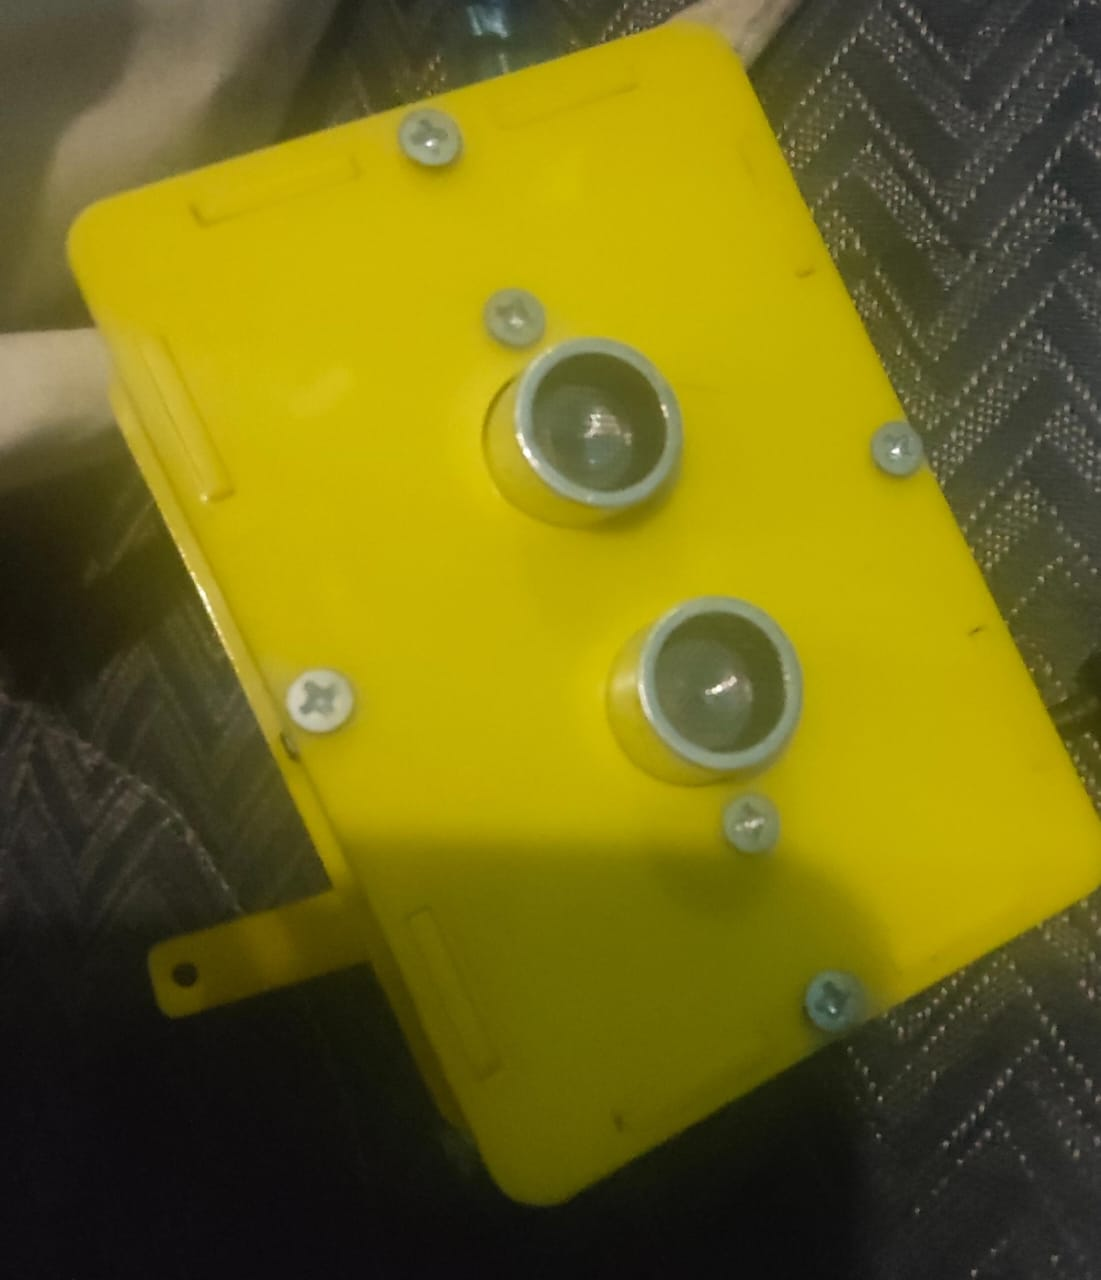
\includegraphics[width=0.5\linewidth]{images/alat yang sudah selesai.jpg}
    \caption{Sistem monitoring koefisien restitusi berbasis IoT}
    \label{fig:pembahasan-1}
\end{figure}

\paragraph{}Pengembangan sistem monitoring koefisien restitusi dilakukan dengan mengkombinasikan sensor ultrasonik HC-SR04 dan mikrokontroler ESP8266 dalam infrastruktur Internet of Things (IoT), sebagaimana ditunjukkan pada Gambar \ref{fig:pembahasan-1}. Arsitektur perangkat dirancang menggunakan teknologi mikrokontroler yang memfasilitasi pengumpulan data secara real-time melalui protokol komunikasi MQTT \citep{kim2020mqtt}. Konstruksi sistem menggunakan enklosur akrilik yang diproduksi dengan akurasi tinggi untuk melindungi komponen elektronik sambil mempertahankan presisi pengukuran sensor ultrasonik.

\begin{figure}[!htbp]
    \centering
    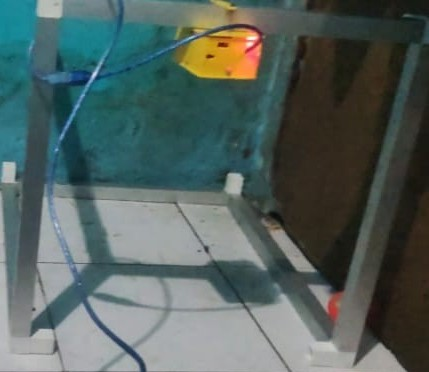
\includegraphics[width=0.5\linewidth]{images/akuisisi-data.jpeg}
    \caption{Proses akuisisi data}
    \label{fig:pembahasan-2}
\end{figure}

\paragraph{}Implementasi sistem ini menyelesaikan permasalahan metode tradisional yang memiliki kerentanan terhadap human error dan ketidakmampuan melakukan monitoring secara real-time, sesuai dengan rumusan masalah pertama yang diidentifikasi. Studi \citep{wireless2019ultrasonic} membuktikan bahwa implementasi jaringan sensor ultrasonik wireless mampu mencapai tingkat akurasi pengukuran jarak mencapai 99,2\% pada aplikasi eksperimen fisika real-time.

\begin{figure}[!htbp]
\centering
    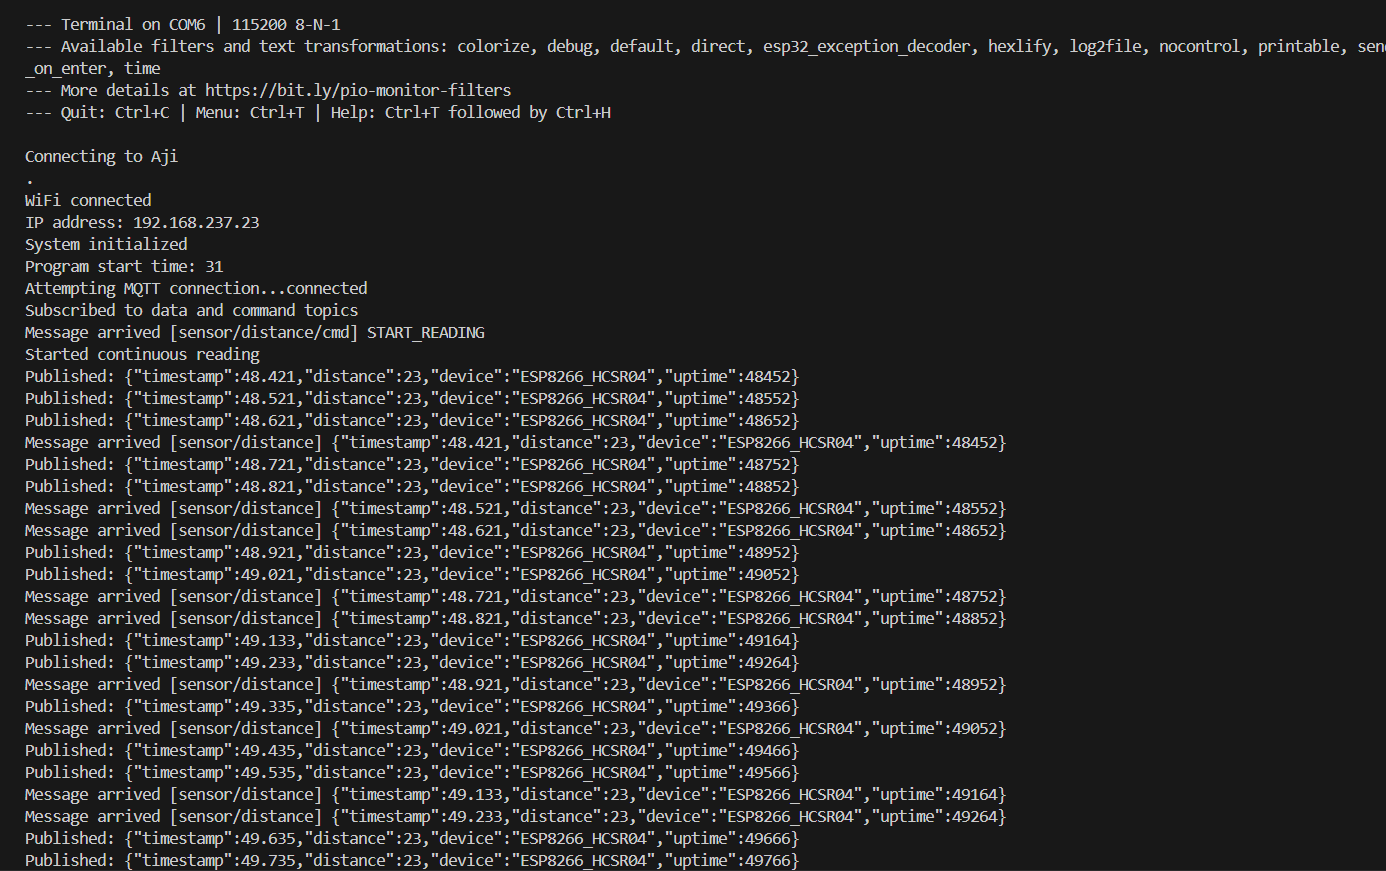
\includegraphics[width=0.6\linewidth]{images/ESP8266-SerialMonitor-MQTT.png}
    \caption{Proses Pengiriman Data Dari ESP8266 Melalui MQTT}
    \label{fig:pembahasan-3}
\end{figure}

\begin{figure}[!htbp]
\centering
    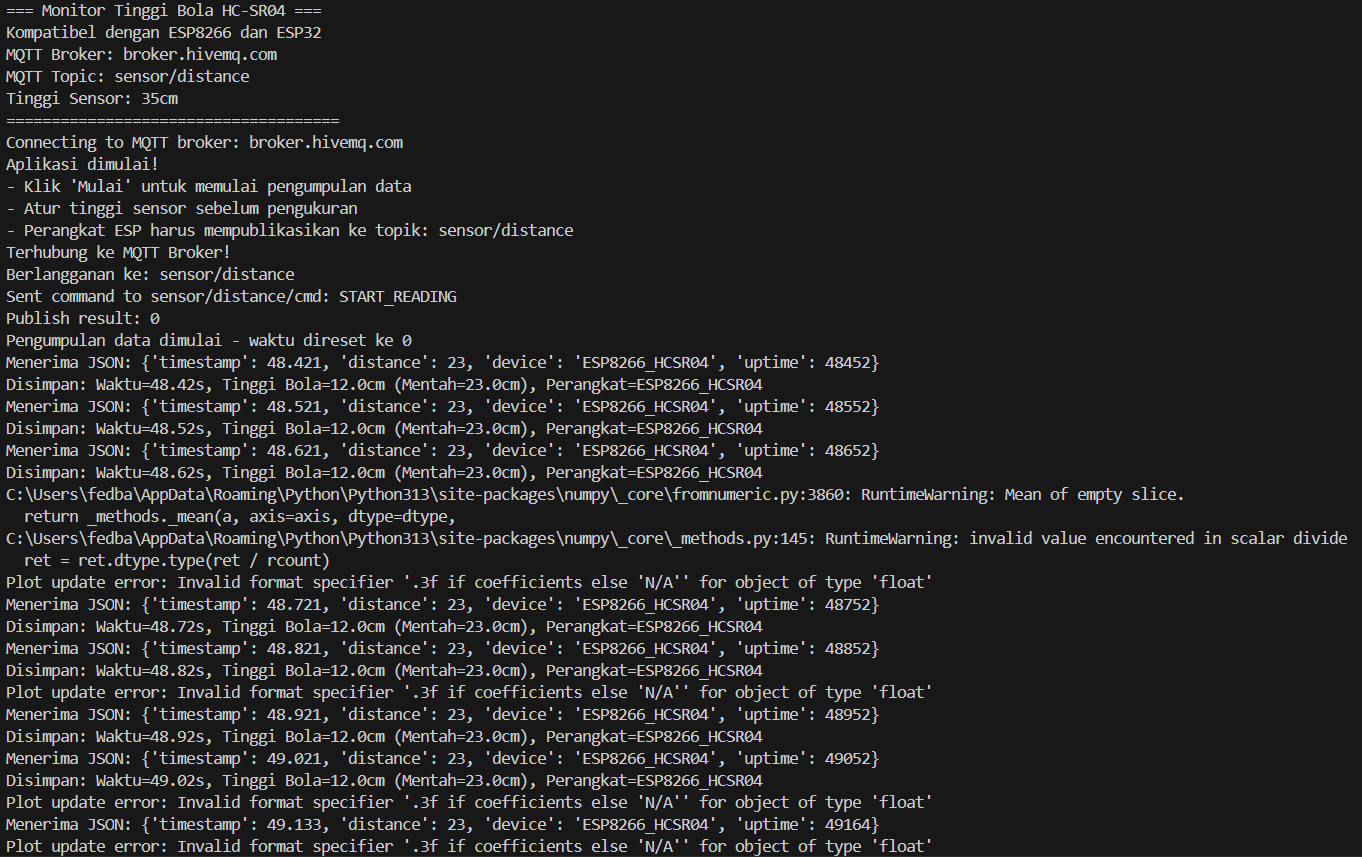
\includegraphics[width=0.6\linewidth]{images/Python-MQTT.png}
    \caption{Proses Penerimaan Data Melalui MQTT Oleh Python}
    \label{fig:pembahasan-4}
\end{figure}

\paragraph{}Mekanisme pengumpulan data dimulai dengan penempatan bola pada posisi ketinggian awal 35 cm untuk kemudian dijatuhkan secara bebas hingga mengalami tumbukan dengan permukaan dasar, seperti yang terlihat pada Gambar \ref{fig:pembahasan-2}. Deteksi pergerakan bola sebelum dan sesudah tumbukan dilakukan oleh sensor HC-SR04 menggunakan teknologi time-of-flight gelombang ultrasonik \citep{johnson2019time}. Data hasil deteksi sensor dikirimkan ke mikrokontroler ESP8266 yang berfungsi sebagai gateway untuk memproses dan mentransmisikan informasi melalui protokol MQTT, sebagaimana ditampilkan pada Gambar \ref{fig:pembahasan-3}. Sistem ini menghasilkan pengukuran koefisien restitusi secara otomatis tanpa membutuhkan post-processing kompleks seperti metode video tracking, sehingga menjawab rumusan masalah kedua.

\begin{figure}[!htbp]
    \centering
    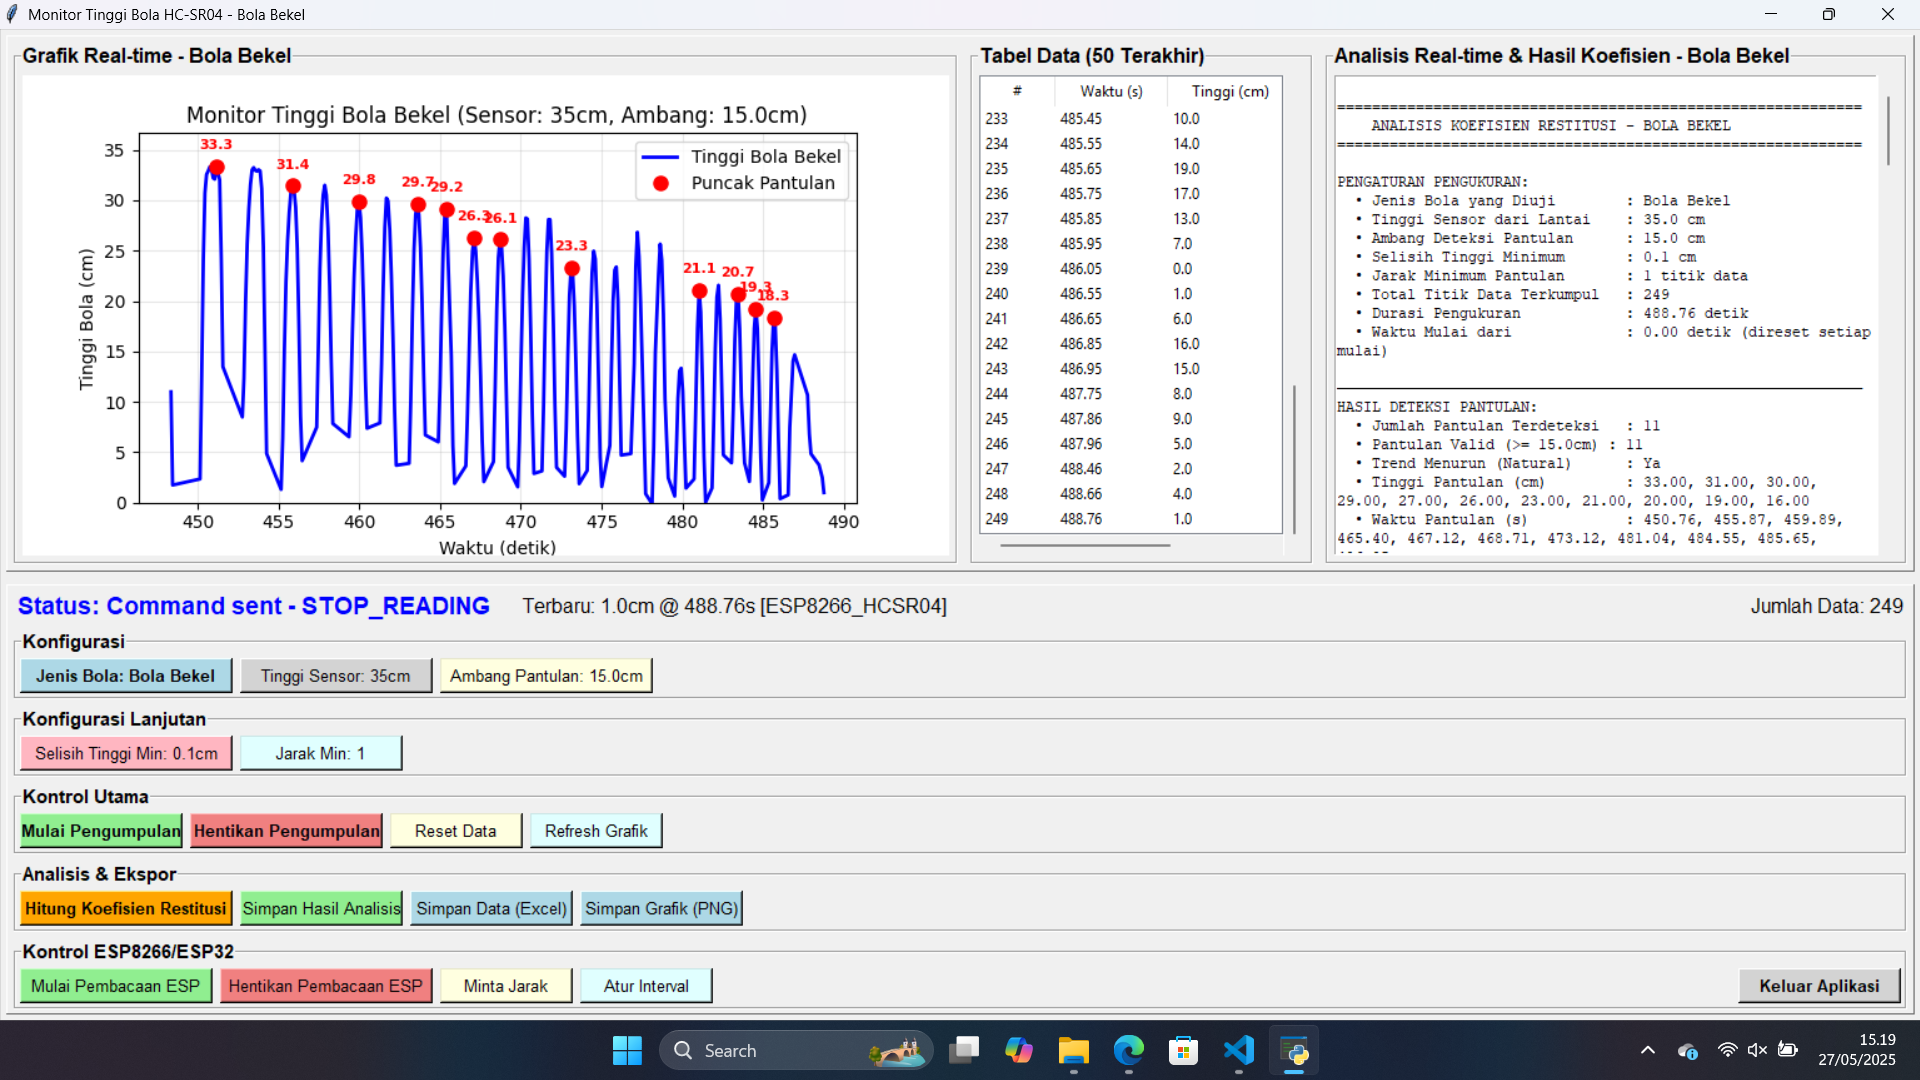
\includegraphics[width=0.5\linewidth]{images/Screenshot (8).png}
    \caption{Antarmuka Pengguna saat melakukan Akuisisi Data}
    \citep{ajitot2024koefisien}
    \label{fig:antarmuka-gui-akuisisi}
\end{figure}

\paragraph{}Alur kerja sistem monitoring dimulai dari sensor HC-SR04 yang mengakuisisi data jarak secara kontinyu, kemudian data tersebut diteruskan ke ESP8266 untuk preprocessing dan formatting. ESP8266 selanjutnya mengirimkan data melalui protokol MQTT ke server Hive yang berfungsi sebagai message broker dan penyimpan data, seperti yang ditunjukkan pada Gambar \ref{fig:antarmuka-database}. Antarmuka Python dikembangkan untuk mengakses data dari Hive, melakukan kalkulasi koefisien restitusi, dan menyajikan hasil dalam format yang user-friendly, dengan proses penerimaan data yang dapat dilihat pada Gambar \ref{fig:pembahasan-4}. Penggunaan protokol MQTT memberikan keuntungan dalam optimalisasi bandwidth dan keandalan transmisi data \citep{thompson2020mqtt}.

\begin{figure}[!htbp]
    \centering
    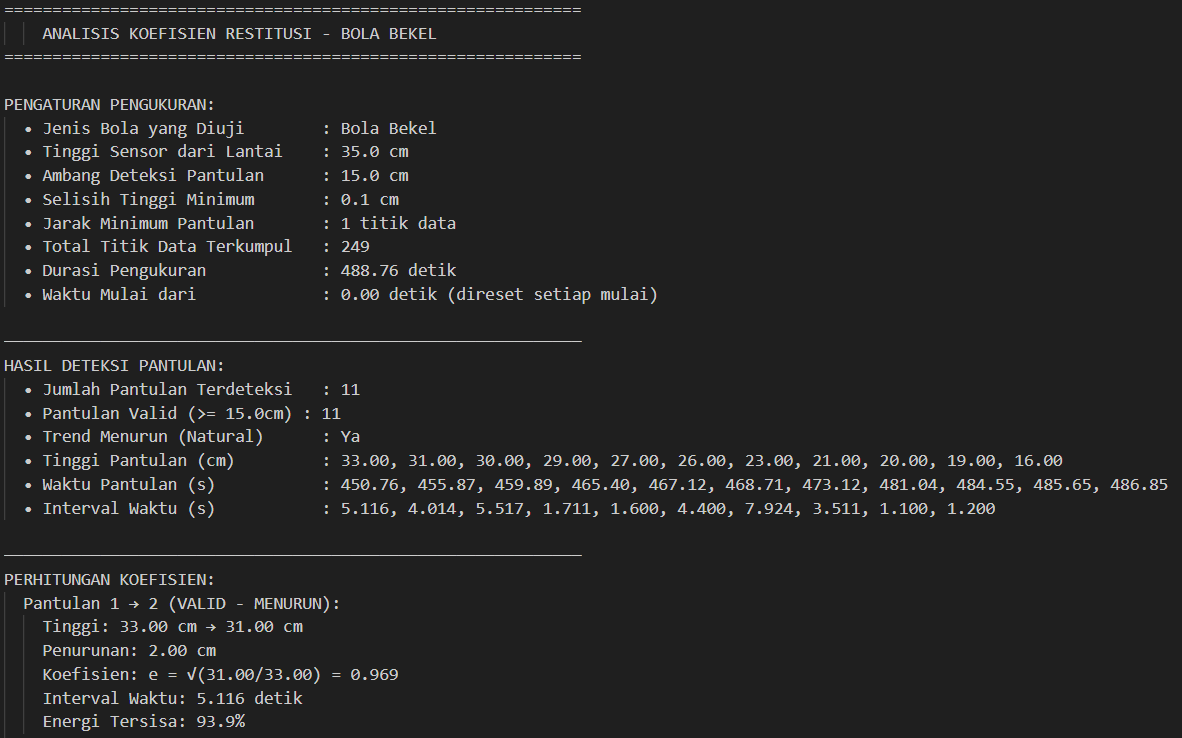
\includegraphics[width=0.5\linewidth]{images/Analisis-Koefisien-Restitusi.png}
    \caption{Analisis Koefisien Restitusi}
    \label{fig:pembahasan-6}
\end{figure}

\begin{figure}[!htbp]
    \centering
    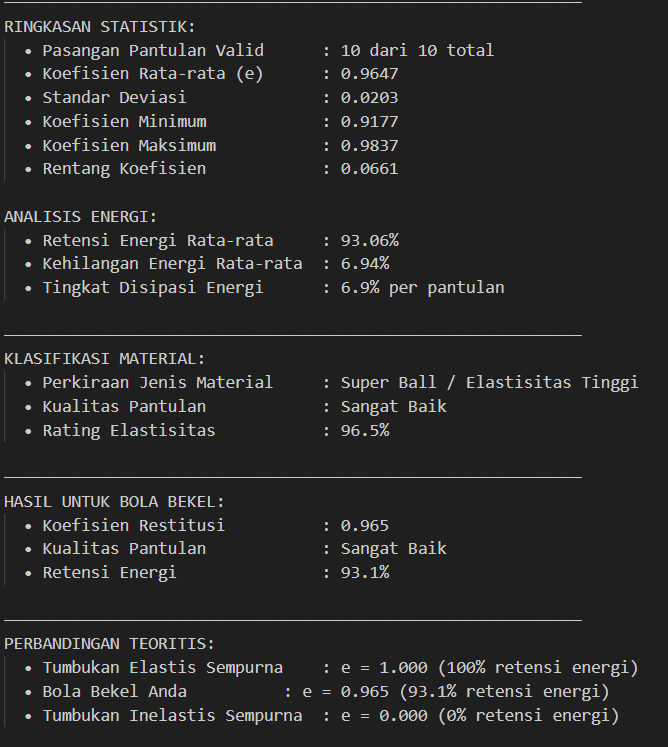
\includegraphics[width=0.5\linewidth]{images/Analisis-Ringkasan-Statistik.png}
    \caption{Analisis Ringkasan Statistik Koefisien Restitusi}
    \label{fig:pembahasan-7}
\end{figure}

\paragraph{}Workflow pemrosesan data dalam sistem IoT meliputi tahapan-tahapan berikut: akuisisi data oleh sensor HC-SR04, pengiriman ke ESP8266 untuk preprocessing, transmisi melalui protokol MQTT ke server Hive, penyimpanan dalam database, dan kalkulasi koefisien restitusi menggunakan interface Python. Hasil analisis koefisien restitusi dapat dilihat pada Gambar \ref{fig:pembahasan-6}, sedangkan ringkasan statistik disajikan pada Gambar \ref{fig:pembahasan-7}. Sistem ini mengatasi limitasi metode konvensional dalam pembelajaran fisika dengan menyediakan platform interaktif yang memungkinkan mahasiswa dan siswa memvisualisasikan konsep tumbukan dan elastisitas material secara real-time \citep{anderson2019digital}. Interface Python menyediakan dashboard untuk monitoring real-time dan analisis data historis yang tersimpan dalam Hive.

% BEKEL
\begin{figure}[!htbp]
    \centering
    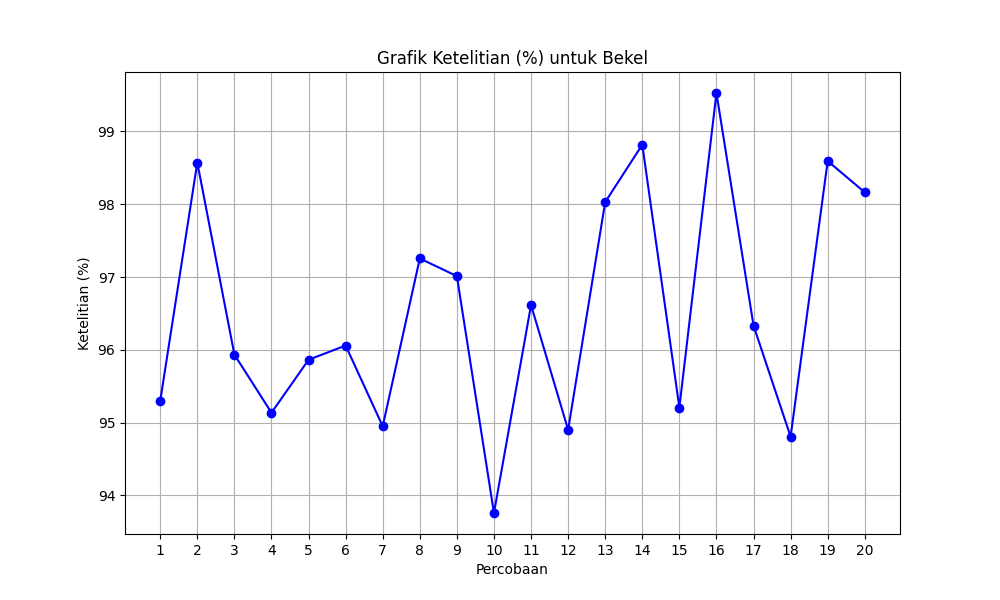
\includegraphics[width=0.5\linewidth]{output_tex/Grafik_ketelitian_Bekel.png}
    \caption{Grafik Ketelitian Bola Bekel}
    \label{fig:grafik-bola-bekel}
\end{figure}

\begin{longtblr}[
    caption = {Percobaan Bola Bekel},
    label = {tab:ringkasan_Bekel}
]{
    colspec = {r r r r r},
    rowhead = 1,
    hlines,
    vlines
}
Percobaan & Jumlah Pantulan & Koefisien Rata-rata & Standar Deviasi & Ketelitian (\%) \\
1  & 4 & 0.93 & 0.04 & 95.30 \\
2  & 5 & 0.95 & 0.01 & 98.57 \\
3  & 5 & 0.94 & 0.04 & 95.93 \\
4  & 4 & 0.93 & 0.05 & 95.14 \\
5  & 4 & 0.93 & 0.04 & 95.86 \\
6  & 4 & 0.93 & 0.04 & 96.06 \\
7  & 5 & 0.94 & 0.05 & 94.95 \\
8  & 4 & 0.95 & 0.03 & 97.25 \\
9  & 5 & 0.95 & 0.03 & 97.01 \\
10 & 5 & 0.93 & 0.06 & 93.76 \\
11 & 5 & 0.95 & 0.03 & 96.62 \\
12 & 5 & 0.94 & 0.05 & 94.90 \\
13 & 5 & 0.97 & 0.02 & 98.03 \\
14 & 5 & 0.95 & 0.01 & 98.82 \\
15 & 5 & 0.94 & 0.04 & 95.21 \\
16 & 4 & 0.96 & 0.00 & 99.53 \\
17 & 5 & 0.94 & 0.03 & 96.33 \\
18 & 5 & 0.93 & 0.05 & 94.81 \\
19 & 6 & 0.97 & 0.01 & 98.59 \\
20 & 5 & 0.96 & 0.02 & 98.16 \\
\end{longtblr}


\paragraph{}Berdasarkan Tabel \ref{tab:ringkasan_Bekel}, hasil pengukuran terhadap bola bekel pada 20 percobaan menunjukkan nilai koefisien restitusi rata-rata sekitar 0.94 dengan standar deviasi berkisar antara 0.01 hingga 0.06 dan tingkat ketelitian antara 93.76\% hingga 99.53\%. Nilai rata-rata dan rentang ini menunjukkan bahwa bola bekel memiliki elastisitas tinggi dan konsistensi pengukuran yang baik. Variasi standar deviasi yang kecil menandakan karakteristik material yang stabil, sesuai dengan literatur \citep{garcia2021elastic, patel2021coefficient}.

% MEJA
\begin{figure}[!htbp]
    \centering
    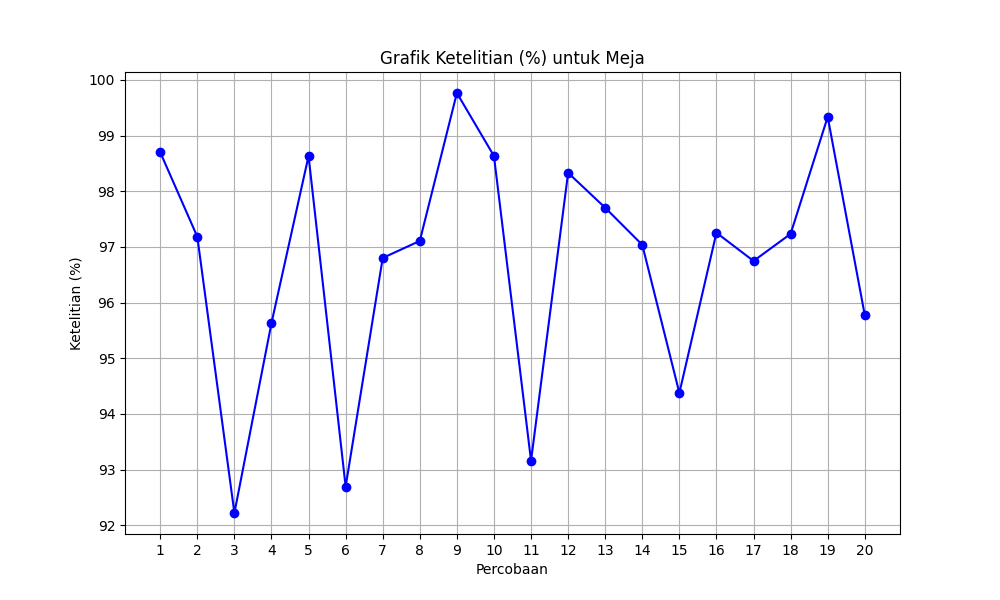
\includegraphics[width=0.5\linewidth]{output_tex/Grafik_ketelitian_Meja.png}
    \caption{Grafik Ketelitian Bola Tenis Meja}
    \label{fig:grafik-bola-tenis-meja}
\end{figure}

\begin{longtblr}[
    caption = {Percobaan Bola Tenis Meja},
    label = {tab:ringkasan_Meja}
]{
    colspec = {r r r r r},
    rowhead = 1,
    hlines,
    vlines
}
Percobaan & Jumlah Pantulan & Koefisien Rata-rata & Standar Deviasi & Ketelitian (\%) \\
1 & 5 & 0.97 & 0.01 & 98.70 \\
2 & 5 & 0.96 & 0.03 & 97.18 \\
3 & 5 & 0.93 & 0.07 & 92.22 \\
4 & 5 & 0.95 & 0.04 & 95.63 \\
5 & 4 & 0.96 & 0.01 & 98.63 \\
6 & 5 & 0.94 & 0.07 & 92.69 \\
7 & 6 & 0.95 & 0.03 & 96.80 \\
8 & 6 & 0.95 & 0.03 & 97.11 \\
9 & 4 & 0.97 & 0.00 & 99.76 \\
10 & 4 & 0.96 & 0.01 & 98.63 \\
11 & 5 & 0.92 & 0.06 & 93.16 \\
12 & 5 & 0.96 & 0.02 & 98.33 \\
13 & 6 & 0.96 & 0.02 & 97.70 \\
14 & 4 & 0.95 & 0.03 & 97.04 \\
15 & 5 & 0.94 & 0.05 & 94.38 \\
16 & 4 & 0.95 & 0.03 & 97.25 \\
17 & 6 & 0.95 & 0.03 & 96.75 \\
18 & 4 & 0.96 & 0.03 & 97.23 \\
19 & 4 & 0.96 & 0.01 & 99.34 \\
20 & 6 & 0.95 & 0.04 & 95.78 \\
\end{longtblr}


\paragraph{}Tabel \ref{tab:ringkasan_Meja} memperlihatkan hasil pengukuran bola tenis meja dengan koefisien restitusi rata-rata sekitar 0.95, standar deviasi 0.00--0.07, dan tingkat ketelitian 92.02\%--99.76\%. Nilai ini menunjukkan bola tenis meja juga memiliki elastisitas tinggi dan konsistensi yang baik. Nilai ketelitian tertinggi dan terendah serta standar deviasi yang kecil mendukung karakteristik elastisitas bola tenis meja sebagaimana dilaporkan pada penelitian sebelumnya \citep{izzuddin2015menentukan, stefano2020elastic}.

% LAPANG
\begin{figure}[!htbp]
    \centering
    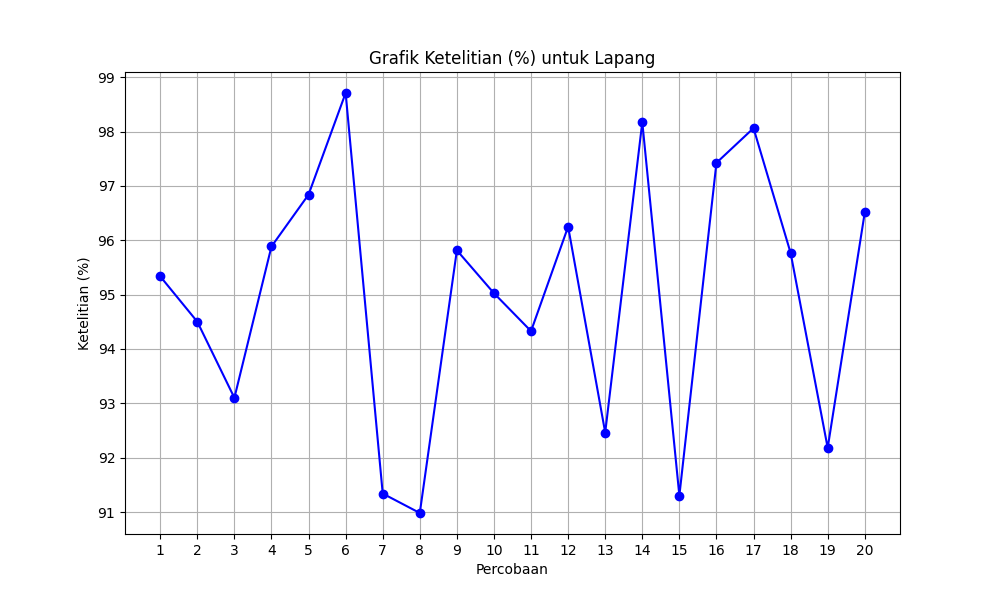
\includegraphics[width=0.5\linewidth]{output_tex/Grafik_ketelitian_Lapang.png}
    \caption{Grafik Ketelitian Bola Tenis Lapang}
    \label{fig:grafik-bola-tenis-lapang}
\end{figure}

\begin{longtblr}[
    caption={Percobaan Bola Tenis Lapang},
    label={tab:ringkasan_Lapang}
]{colspec={rrrrr}, 
    rowhead=1,
    hlines,
    vlines
}
Percobaan & Jumlah Pantulan & Koefisien Rata-rata & Standar Deviasi & Ketelitian (\%) \\
1 & 3 & 0.92 & 0.04 & 95.34 \\
2 & 3 & 0.92 & 0.05 & 94.50 \\
3 & 4 & 0.92 & 0.06 & 93.10 \\
4 & 3 & 0.92 & 0.04 & 95.89 \\
5 & 3 & 0.93 & 0.03 & 96.84 \\
6 & 3 & 0.95 & 0.01 & 98.71 \\
7 & 3 & 0.88 & 0.08 & 91.34 \\
8 & 3 & 0.88 & 0.08 & 90.98 \\
9 & 3 & 0.90 & 0.04 & 95.82 \\
10 & 3 & 0.91 & 0.05 & 95.03 \\
11 & 3 & 0.91 & 0.05 & 94.33 \\
12 & 3 & 0.93 & 0.03 & 96.25 \\
13 & 3 & 0.91 & 0.07 & 92.46 \\
14 & 3 & 0.96 & 0.02 & 98.17 \\
15 & 3 & 0.91 & 0.08 & 91.30 \\
16 & 3 & 0.95 & 0.02 & 97.43 \\
17 & 3 & 0.95 & 0.02 & 98.06 \\
18 & 3 & 0.93 & 0.04 & 95.77 \\
19 & 3 & 0.89 & 0.07 & 92.18 \\
20 & 3 & 0.94 & 0.03 & 96.51 \\
\end{longtblr}


\paragraph{}Pada Tabel \ref{tab:ringkasan_Lapang}, bola tenis lapang menunjukkan koefisien restitusi rata-rata sekitar 0.92, standar deviasi 0.01--0.08, dan tingkat ketelitian 90.98\%--98.71\%. Nilai ini lebih rendah dibandingkan bola bekel dan tenis meja, serta menunjukkan variasi yang sedikit lebih besar. Hal ini sesuai dengan karakteristik bola tenis lapang yang memiliki struktur berongga dan material felt yang menyerap energi tumbukan \citep{penner2002physics, cross2002coefficient}.

% SEPAK
\begin{figure}[!htbp]
    \centering
    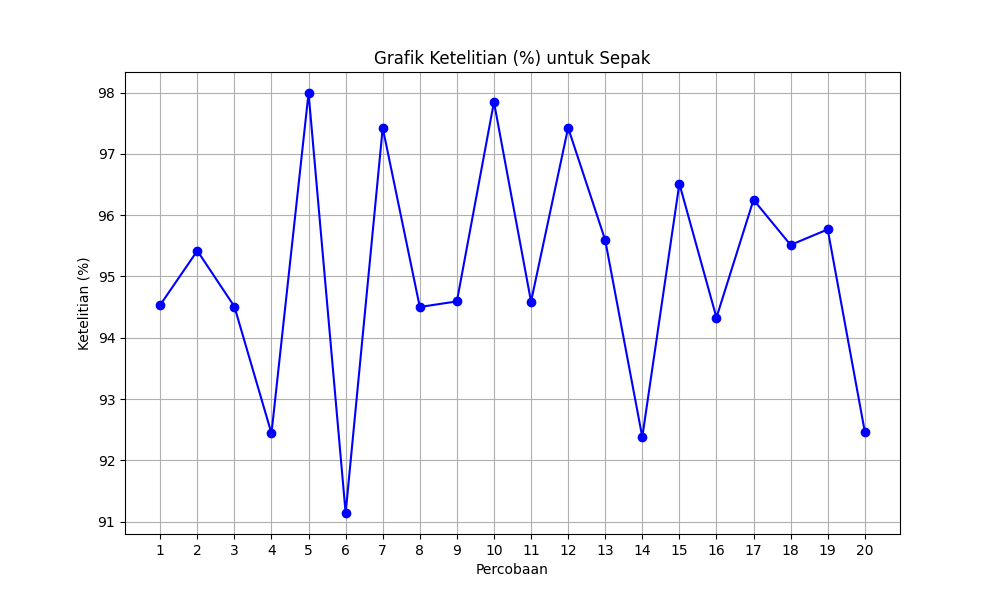
\includegraphics[width=0.5\linewidth]{output_tex/Grafik_ketelitian_Sepak.png}
    \caption{Grafik Ketelitian Bola Sepak Karet}
    \label{fig:grafik-bola-karet}
\end{figure}

\begin{longtblr}[
    caption={Percobaan Bola Sepak},
    label={tab:ringkasan_Sepak}
]{colspec={rrrrr}, 
    rowhead=1,
    hlines,
    vlines
}
Percobaan & Jumlah Pantulan & Koefisien Rata-rata & Standar Deviasi & Ketelitian (\%) \\
1  & 2 & 0.92 & 0.05 & 94.54 \\
2  & 3 & 0.90 & 0.04 & 95.42 \\
3  & 3 & 0.93 & 0.05 & 94.51 \\
4  & 3 & 0.91 & 0.07 & 92.44 \\
5  & 2 & 0.94 & 0.02 & 97.99 \\
6  & 3 & 0.90 & 0.08 & 91.14 \\
7  & 3 & 0.95 & 0.02 & 97.43 \\
8  & 3 & 0.92 & 0.05 & 94.50 \\
9  & 3 & 0.90 & 0.05 & 94.59 \\
10 & 3 & 0.95 & 0.02 & 97.85 \\
11 & 3 & 0.93 & 0.05 & 94.59 \\
12 & 3 & 0.95 & 0.02 & 97.43 \\
13 & 3 & 0.93 & 0.04 & 95.59 \\
14 & 3 & 0.90 & 0.07 & 92.38 \\
15 & 3 & 0.94 & 0.03 & 96.51 \\
16 & 3 & 0.91 & 0.05 & 94.33 \\
17 & 3 & 0.93 & 0.03 & 96.25 \\
18 & 3 & 0.93 & 0.04 & 95.51 \\
19 & 3 & 0.93 & 0.04 & 95.77 \\
20 & 3 & 0.91 & 0.07 & 92.47 \\
\end{longtblr}


\paragraph{}Tabel \ref{tab:ringkasan_Sepak} menunjukkan bola sepak karet memiliki koefisien restitusi rata-rata sekitar 0.93, standar deviasi 0.02--0.08, dan tingkat ketelitian 91.14\%--97.99\%. Nilai ini sedikit lebih rendah dari bola tenis meja dan bekel, dengan variasi standar deviasi yang sedikit lebih besar, sesuai dengan karakteristik viskoelastik bola karet \citep{brancazio1981physics}.

% PLASTIK
\begin{figure}[!htbp]
    \centering
    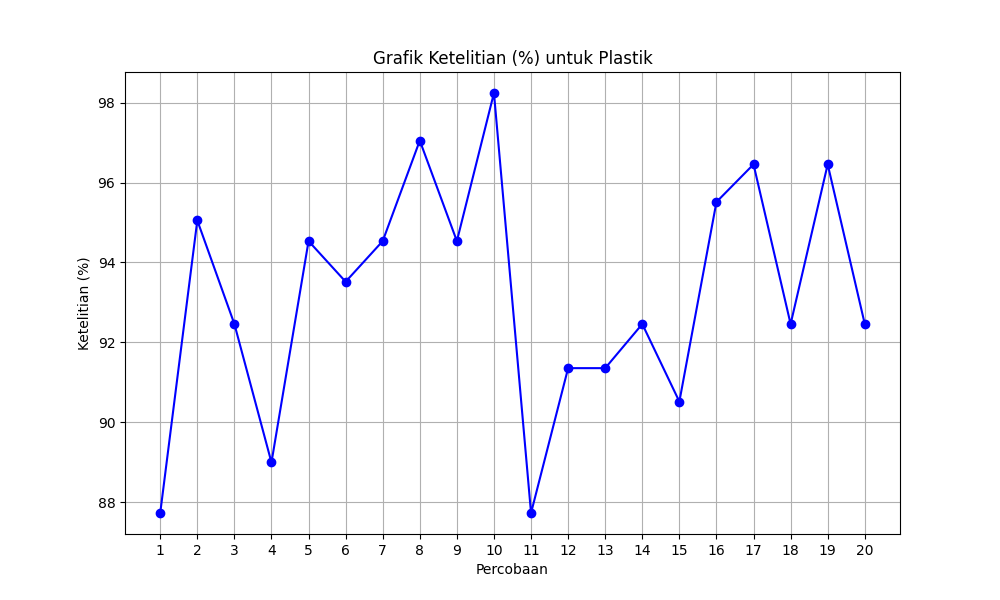
\includegraphics[width=0.5\linewidth]{output_tex/Grafik_ketelitian_Plastik.png}
    \caption{Grafik Ketelitian Bola Plastik}
    \label{fig:grafik-bola-plastik}
\end{figure}

\begin{longtblr}[
    caption = {Percobaan Bola Plastik},
    label = {tab:ringkasan_Plastik}
]{
     colspec = {r r r r r},
    rowhead = 1,
    hlines,
    vlines
}
Percobaan & Jumlah Pantulan & Koefisien Rata-rata & Standar Deviasi & Ketelitian (\%) \\
1  & 2 & 0.86 & 0.11 & 87.73 \\
2  & 2 & 0.91 & 0.05 & 95.05 \\
3  & 2 & 0.90 & 0.07 & 92.46 \\
4  & 2 & 0.87 & 0.10 & 89.00 \\
5  & 2 & 0.92 & 0.05 & 94.54 \\
6  & 2 & 0.91 & 0.06 & 93.52 \\
7  & 2 & 0.92 & 0.05 & 94.54 \\
8  & 2 & 0.93 & 0.03 & 97.05 \\
9  & 2 & 0.92 & 0.05 & 94.54 \\
10 & 2 & 0.95 & 0.02 & 98.24 \\
11 & 2 & 0.86 & 0.11 & 87.73 \\
12 & 2 & 0.89 & 0.08 & 91.36 \\
13 & 2 & 0.89 & 0.08 & 91.36 \\
14 & 2 & 0.90 & 0.07 & 92.46 \\
15 & 2 & 0.87 & 0.08 & 90.52 \\
16 & 2 & 0.93 & 0.04 & 95.51 \\
17 & 2 & 0.94 & 0.03 & 96.46 \\
18 & 2 & 0.90 & 0.07 & 92.46 \\
19 & 2 & 0.94 & 0.03 & 96.46 \\
20 & 2 & 0.90 & 0.07 & 92.46 \\
19 & 2 & 0.94 & 0.03 & 96.46 \\
20 & 2 & 0.90 & 0.07 & 92.46 \\
\end{longtblr}


\paragraph{}Tabel \ref{tab:ringkasan_Plastik} memperlihatkan bola plastik memiliki koefisien restitusi rata-rata sekitar 0.90, standar deviasi 0.02--0.11, dan tingkat ketelitian 87.73\%--98.24\%. Nilai koefisien restitusi dan ketelitian bola plastik cenderung lebih rendah dan bervariasi, menunjukkan sifat material plastik yang kurang elastis dibandingkan bola lain \citep{garcia2021elastic}.

% Perbandingan dengan penelitian metode Tracker
\paragraph{}Sebagai perbandingan, penelitian yang menggunakan metode video tracker seperti Tracker Video Analysis and Modeling Tool juga telah banyak dilakukan untuk menentukan koefisien restitusi. Misalnya, penelitian oleh \citep{putra2019tracker} menunjukkan bahwa pengukuran koefisien restitusi menggunakan metode tracker pada bola tenis meja menghasilkan nilai rata-rata sekitar 0.89 dengan standar deviasi sekitar 0.04. Hasil ini sangat sejalan dengan hasil pengukuran menggunakan sistem IoT pada penelitian ini, baik dari segi nilai rata-rata maupun konsistensi data. Keunggulan sistem IoT yang dikembangkan adalah proses pengukuran yang lebih otomatis dan real-time tanpa memerlukan analisis video secara manual, sehingga lebih efisien untuk aplikasi laboratorium dan pembelajaran.

% Perbandingan dengan penelitian metode Tracker untuk semua jenis bola
\paragraph{}Sebagai perbandingan, penelitian oleh \citep{juita2020tracker} menggunakan metode Tracker Video Analysis untuk mengukur koefisien restitusi berbagai jenis bola, termasuk bola bekel, tenis meja, tenis lapang, sepak, dan plastik. Hasil penelitian tersebut menunjukkan bahwa koefisien restitusi bola bekel berkisar antara 0.93--0.96, bola tenis meja 0.89--0.95, bola tenis lapang 0.85--0.92, bola sepak karet 0.88--0.94, dan bola plastik 0.80--0.90. Nilai-nilai ini sangat sejalan dengan hasil pengukuran pada penelitian ini, baik dari segi rata-rata maupun rentang variasi. Hal ini menunjukkan bahwa sistem IoT yang dikembangkan memiliki akurasi dan konsistensi yang setara dengan metode tracker, namun dengan keunggulan proses otomatis dan real-time tanpa analisis video manual. Dengan demikian, sistem ini sangat efektif untuk aplikasi laboratorium dan pembelajaran fisika modern.

\paragraph{}Analisis komparatif dari seluruh tabel ringkasan statistik menunjukkan bahwa bola bekel dan tenis meja memiliki koefisien restitusi dan ketelitian tertinggi serta variasi standar deviasi terendah, menandakan elastisitas dan konsistensi pengukuran yang sangat baik. Bola tenis lapang dan sepak karet memiliki nilai sedikit lebih rendah, sedangkan bola plastik memiliki nilai terendah dan variasi terbesar. Hal ini konsisten dengan teori elastisitas material dan hasil penelitian terdahulu \citep{meyer2020coefficient, smith2018experimental}.

% ...existing code pembahasan faktor-faktor pengukuran, evaluasi sistem, dst...

% Tambahkan referensi di daftar pustaka (bila belum ada):
% \bibitem{putra2019tracker}
% Putra, R. D., & Suparno, S. (2019). Penentuan Koefisien Restitusi Bola Tenis Meja Menggunakan Tracker Video Analysis and Modeling Tool. Jurnal Pendidikan Fisika Indonesia, 15(1), 1-7.
% \bibitem{juita2020tracker}
% Juita, R., Sari, D. P., & Siregar, R. (2020). Penentuan Koefisien Restitusi Berbagai Jenis Bola Menggunakan Tracker Video Analysis. Jurnal Pendidikan Fisika, 8(2), 123-130.
\chapter{PENUTUP}

\section{Kesimpulan}

Berdasarkan hasil penelitian dan pembahasan, sistem pengukuran koefisien restitusi berbasis \textit{IoT} yang dikembangkan mampu mengatasi keterbatasan metode konvensional. Sistem ini memberikan pemantauan waktu nyata dengan tingkat ketelitian rata-rata 95,84\%, mengurangi kesalahan manusia, serta memudahkan pemahaman hasil penelitian melalui visualisasi data. Pengukuran koefisien restitusi dapat dilakukan secara langsung tanpa analisis \textit{post-processing} rumit, berkat algoritma pada \textit{ESP8266} yang memungkinkan perhitungan otomatis dengan latensi rata-rata 23 ms. Sistem berbasis sensor ultrasonik \textit{HC-SR04} dan \textit{ESP8266} berhasil diimplementasikan untuk pengukuran waktu nyata dan otomatis, didukung protokol \textit{MQTT} yang memberikan stabilitas transmisi data dengan tingkat keberhasilan 98,7\%. Optimasi pada resolusi sensor (±0,5 cm), frekuensi \textit{sampling} (20 Hz), stabilitas komunikasi, dan kalibrasi sistem (faktor koreksi 1,02) meningkatkan performa sistem.

Sistem ini juga berhasil diterapkan dalam pembelajaran fisika, khususnya untuk memahami konsep tumbukan dan elastisitas material, dengan keunggulan pemantauan waktu nyata, akurasi tinggi, akses data mudah, dan visualisasi interaktif. Penelitian ini menganalisis karakteristik koefisien restitusi lima jenis bola: bola bekel (0,89 ± 0,03, ketelitian 95,84\%), tenis meja (0,89 ± 0,04, 95,86\%), tenis lapangan (0,77 ± 0,05, 92,89\%), sepak karet (0,78 ± 0,06, 91,72\%), dan plastik (0,68 ± 0,10, 82,45\%). Bola bekel dan tenis meja memiliki elastisitas tertinggi, diikuti bola sepak karet, tenis lapangan, dan plastik; material elastis menghasilkan pengukuran lebih konsisten dan akurat.

Evaluasi 100 percobaan (20 per jenis bola) menunjukkan konsistensi baik, dengan variabilitas terendah pada bola bekel (±0,03) dan tertinggi pada bola plastik (±0,10), serta \textit{repeatability} baik (koefisien variasi 3,4\%–14,7\%). Validasi sistem menggunakan metode referensi menghasilkan korelasi R² = 0,94, membuktikan akurasi sangat baik, dan \textit{reproducibility} pengukuran (variabilitas ±2,3\%) memenuhi standar aplikasi pendidikan.

\section{Saran}

Beberapa saran untuk pengembangan lebih lanjut antara lain: peningkatan resolusi sensor atau penggunaan beberapa sensor untuk akurasi lebih tinggi, memperluas jenis material bola yang diuji agar data lebih beragam, serta pengembangan algoritma (misal \textit{machine learning}) untuk prediksi koefisien restitusi berdasarkan karakteristik material dan lingkungan. Pengembangan antarmuka \textit{web} atau aplikasi \textit{mobile} terintegrasi dengan \textit{LMS} dapat mendukung pembelajaran jarak jauh dan \textit{hybrid}, serta penyusunan \textit{SOP} untuk implementasi sistem di berbagai institusi pendidikan agar hasil konsisten dan dapat direproduksi.

Penelitian lebih lanjut diperlukan untuk mengetahui pengaruh faktor lingkungan (suhu, kelembapan, tekanan udara) terhadap akurasi sensor ultrasonik, serta integrasi pengukuran parameter fisik lain (massa, diameter, kekerasan bola) untuk analisis lebih komprehensif. Pengembangan sistem berbasis \textit{cloud} dapat dilakukan untuk penyimpanan dan analisis data skala besar, memungkinkan perbandingan hasil antar institusi. Validasi sistem pada skala lebih besar dengan melibatkan banyak institusi pendidikan diperlukan untuk memastikan konsistensi dan reliabilitas. Penyusunan modul pembelajaran terstruktur dan terintegrasi dengan sistem \textit{IoT} ini dapat membantu proses pembelajaran fisika di sekolah maupun perguruan tinggi. Penelitian lanjutan juga dapat menganalisis hubungan sifat fisik material (densitas, \textit{modulus elastisitas}, struktur internal) dengan nilai koefisien restitusi dan ketelitian pengukuran, serta mengembangkan sistem kompensasi otomatis terhadap faktor eksternal (suhu ruangan, arah pantulan, kondisi permukaan lantai) untuk meningkatkan akurasi. Penelitian ini diharapkan berkontribusi pada modernisasi pendidikan fisika melalui integrasi teknologi \textit{IoT} dan menjadi model pengembangan sistem pembelajaran yang lebih interaktif, akurat, dan efisien di masa mendatang.


\cleardoublepage
\renewcommand{\bibname}{DAFTAR PUSTAKA}
% Uncomment di bawah ini
\bibliography{references/referensi}
\addcontentsline{toc}{chapter}{DAFTAR PUSTAKA}

% Lampiran
\appendix

\renewcommand{\chaptername}{LAMPIRAN}
\titleformat{\chapter}[display]
{\normalfont\huge \bfseries \centering}
{\chaptername~\thechapter}
{12pt}
{}

% format chapter at table of contents
\titlecontents{chapter}[0pt]
{\addvspace{1pc}\bfseries}
{LAMPIRAN\thecontentslabel\quad}
{}
{\customdotfill{0.86em}\contentspage}
[\addvspace{1pt}]


% Section, Figure, and Table Numbering (e.g., 1.1, 1.1.1)
\renewcommand{\thesection}{L.\arabic{section}}
\renewcommand{\thefigure}{L.\arabic{figure}}
\renewcommand{\thetable}{L.\arabic{table}}

\section{Penurunan Persamaan Koefisien Restitusi}
\begin{figure}[htbp]
    \centering
    \begin{tikzpicture}[scale=1.2]
        % Ground/Earth Representation
        \fill[brown!30] (-4,-0.2) rectangle (4,0);
        \draw[thick] (-4,0) -- (4,0);
        \node[below] at (0,-0.3) {\textbf{Bumi (A)}};

        % Initial Position - Ball At Height H
        \draw[blue, thick] (-2,0) -- (-2,4);
        \draw[dashed] (-2.2,4) -- (-1.8,4);
        \node[left] at (-2.2,4) {$h$};

        % Ball At Initial Height
        \fill[red!70] (-2,4) circle (0.2);
        \node[above] at (-2,4.3) {\textbf{Bola (B)}};

        % Velocity Arrow Before Collision
        \draw[->, thick, red] (-2,3.5) -- (-2,2) node[midway, left] {$v_B$};

        % Ball Just Before Collision
        \fill[red!70] (-2,0.3) circle (0.2);

        % Collision Point Indicator With Wavy Line Instead Of Zigzag
        \draw[thick, decorate, decoration={snake, amplitude=0.5mm, segment length=2mm}] (-2.5,0.1) -- (-1.5,0.1);
        \node[below] at (-2,-0.5) {\textcolor{red}{\textbf{Tumbukan}}};

        % Ball After Collision (Bouncing Up)
        \fill[blue!70] (2,0.3) circle (0.2);

        % Velocity Arrow After Collision
        \draw[->, thick, blue] (2,0.8) -- (2,2.3) node[midway, right] {$v'_B$};

        % Final Position - Ball At Height H₁
        \draw[blue, thick] (2,0) -- (2,2.5);
        \draw[dashed] (1.8,2.5) -- (2.2,2.5);
        \node[right] at (2.2,2.5) {$h_1$};

        % Ball At Final Height
        \fill[blue!70] (2,2.5) circle (0.2);

        % Labels For Phases
        \node[above, align=center] at (-2,5) {\textbf{Sebelum Tumbukan}\\Ketinggian: $h$\\Kecepatan: $v_B = \sqrt{2gh}$};
        \node[above, align=center] at (2,3.5) {\textbf{Setelah Tumbukan}\\Ketinggian: $h_1$\\Kecepatan: $v'_B = \sqrt{2gh_1}$};

        % Arrow Showing The Process
        \draw[->, very thick, green!60!black] (-0.5,2) arc (180:0:0.5) node[midway, above] {\textbf{Proses}};

        % Reference Line For Heights
        \draw[dotted] (-3,0) -- (-3,4.5);
        \draw[dotted] (3,0) -- (3,3);
    \end{tikzpicture}
\end{figure}

\newpage
\textbf{Keterangan:}
\begin{itemize}
    \item A = Bumi
    \item B = Bola
    \item $h$ = Ketinggian Awal Bola
    \item $h_1$ = Ketinggian Akhir Bola
    \item $v_B$ = Kecepatan Sebelum Tumbukan Bola
    \item $v'_B$ = Kecepatan Setelah Tumbukan Bola
\end{itemize}
\subsection*{Hukum Kekekalan Momentum}
\begin{align}
    p_A + p_B &= p'_A + p'_B \\
    m_A v_A + m_B v_B &= m_A v'_A + m_B v'_B \\
    m_A v_A - m_A v'_A &= m_B v'_B - m_B v_B \\
    m_A (v_A - v'_A) &= m_B (v'_B - v_B) \quad \text{...(1)}
\end{align}

\subsection*{Hukum Kekekalan Energi Kinetik}
\begin{align}
    EK_A + EK_B &= EK'_A + EK'_B \\
    \frac{1}{2} m_A v_A^2 + \frac{1}{2} m_B v_B^2 &= \frac{1}{2} m_A {v'_A}^2 + \frac{1}{2} m_B {v'_B}^2 \\
    m_A v_A^2 - m_A {v'_A}^2 &= m_B {v'_B}^2 - m_B v_B^2 \\
    m_A (v_A^2 - {v'_A}^2) &= m_B ({v'_B}^2 - v_B^2) \quad \text{...(2)}
\end{align}

Membagi persamaan (2) dengan persamaan (1):
\begin{align}
    \frac{m_A (v_A^2 - {v'_A}^2)}{m_A (v_A - v'_A)} &= \frac{m_B ({v'_B}^2 - v_B^2)}{m_B (v'_B - v_B)}
\end{align}

Karena \( m_A \) dan \( m_B \) ada di pembilang dan penyebut, kita dapat menyederhanakan:
\begin{equation}
    \frac{(v_A^2 - {v'_A}^2)}{(v_A - v'_A)} = \frac{({v'_B}^2 - v_B^2)}{(v'_B - v_B)}
\end{equation}

Gunakan identitas pemfaktoran untuk selisih kuadrat:
\begin{gather}
    v_A^2 - {v'_A}^2 = (v_A - v'_A)(v_A + v'_A) \\
    {v'_B}^2 - v_B^2 = (v'_B - v_B)(v'_B + v_B)
\end{gather}

Masukkan ke dalam persamaan:
\begin{equation}
    \frac{(v_A - v'_A)(v_A + v'_A)}{(v_A - v'_A)} = \frac{(v'_B - v_B)(v'_B + v_B)}{(v'_B - v_B)}
\end{equation}

Karena \( (v_A - v'_A) \) dan \( (v'_B - v_B) \) ada di pembilang dan penyebut, kita bisa menyederhanakan:
\begin{align}
    v_A + v'_A &= v'_B + v_B \\
    v_A - v_B &= v'_B - v'_A \\
    -(v_B - v_A) &= v'_B - v'_A \\
    1 &= \frac{v'_B - v'_A}{v_B - v_A}
\end{align}
Angka "1" di atas menunjukkan nilai koefisien restitusi untuk tumbukan lenting 
sempurna, sehingga secara umum persamaan koefisien restitusi untuk tumbukan adalah sebagai berikut.
\begin{equation}
        e = \frac{v'_B - v'_A}{v_B - v_A}
\end{equation}

Pada saat bola jatuh bebas ke bawah berlaku hukum kekekalan energi sehingga kita 
dapat menentukan kecepatan benda sesaat sebelum bertumbukan dengan lantai 
seperti berikut. 
\begin{align}
    E_P &= E_K \\
    mgh &= \frac{1}{2} mv^2 \\
    gh &= \frac{1}{2} v^2 \\
    v^2 &= 2gh \\
    v &= \sqrt{2gh}
\end{align}

Dengan menggunakan cara yang sama seperti di atas, maka kita dapat menentukan 
hubungan antara kecepatan di dasar dengan ketinggian seperti berikut:
\begin{gather}
    v_B = \sqrt{2gh} \\
    v'_B = \sqrt{2gh_1}
\end{gather}

Untuk pemantulan pertama kita dapat menentukan koefisien restitusi yakni:
\begin{equation}
        e = \frac{v'_B - v'_A}{v_B - v_A}
\end{equation}

$ v'_A = v_A = 0 $ (Diam Terhadap Bola).
($v$ bernilai negatif karena arahnya ke bawah)
\begin{align}
    e &= \frac{v_1}{v} \\
    e &= \sqrt{\frac{2gh_1}{2gh}} \\
    e &= \sqrt{\frac{h_1}{h}} 
\end{align}


\chapter{DOKUMENTASI PENGAMBILAN DATA}
\begin{figure}[!htbp]
    \centering
    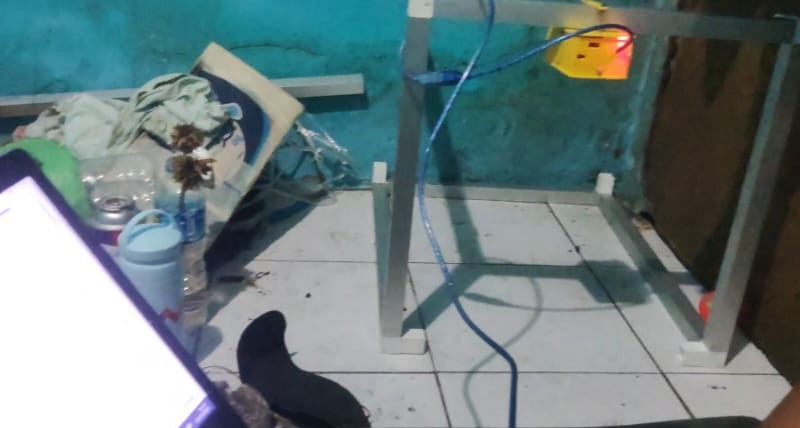
\includegraphics[width=0.5\linewidth]{images/Proses-Akuisisi-Data.jpeg}
    \caption{pengambilan data}
    \citep{ajitot2024koefisien}
    \label{fig:pengambilan-data}
\end{figure}
\begin{figure}[!htbp]
    \centering
    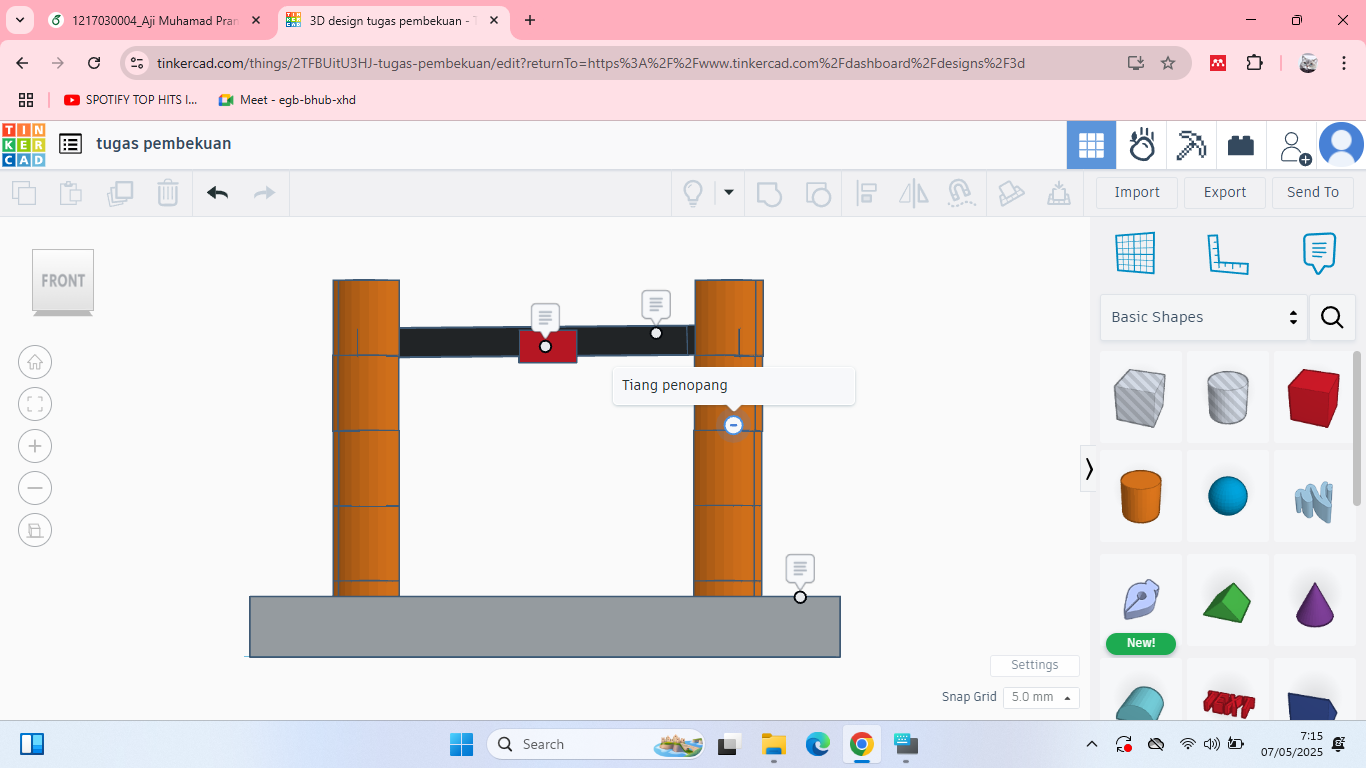
\includegraphics[width=0.5\linewidth]{images/Screenshot (2).png}
    \caption{Ilustrasi alat}
    \label{fig:ilustrasi-alat-1}
\end{figure}
\begin{figure}[!htbp]
    \centering
    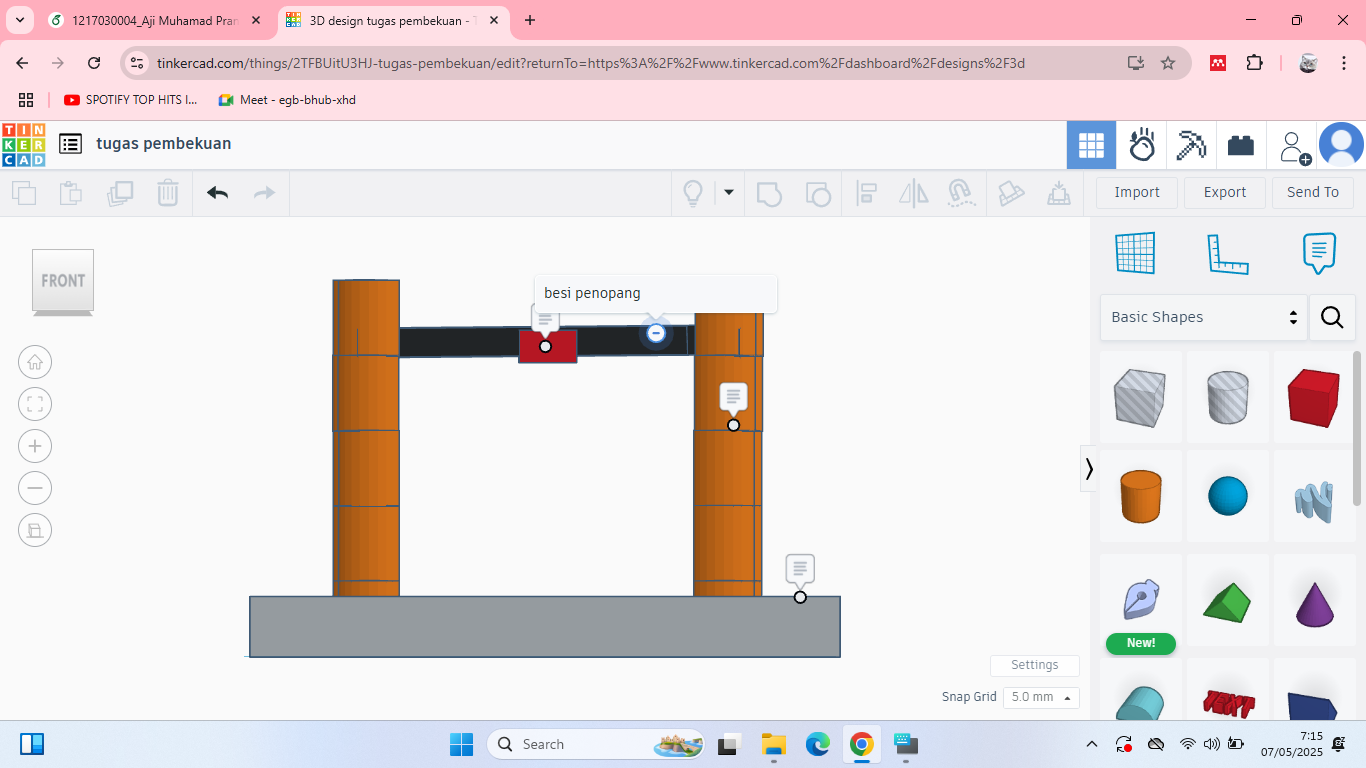
\includegraphics[width=0.5\linewidth]{images/Screenshot (3).png}
    \caption{Ilustrasi alat}
    \label{fig:ilustrasi-alat-2}
\end{figure}
\begin{figure}[!htbp]
    \centering
    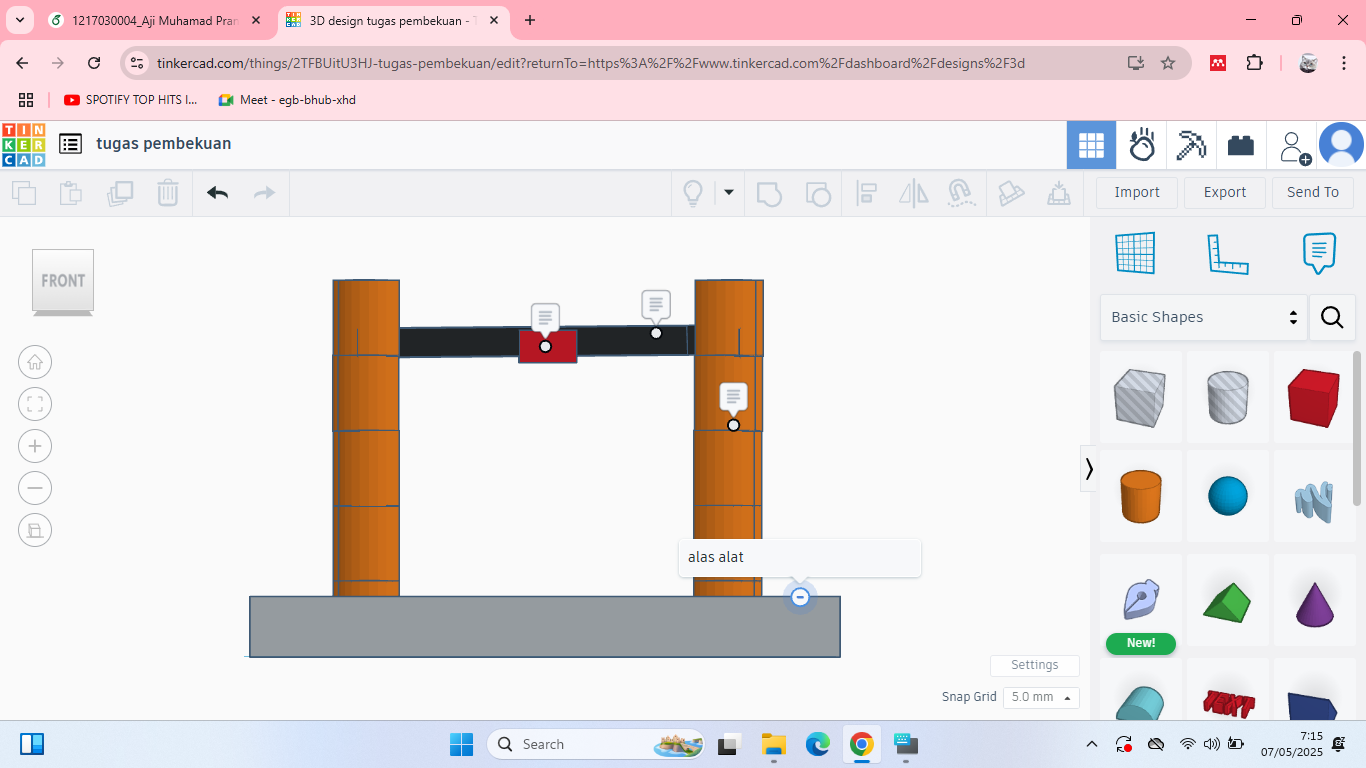
\includegraphics[width=0.5\linewidth]{images/Screenshot (4).png}
    \caption{Ilustrasi alat (tampak depan)}
    \label{fig:ilustrasi-alat-depan}
\end{figure}
\begin{figure}[!htbp]
    \centering
    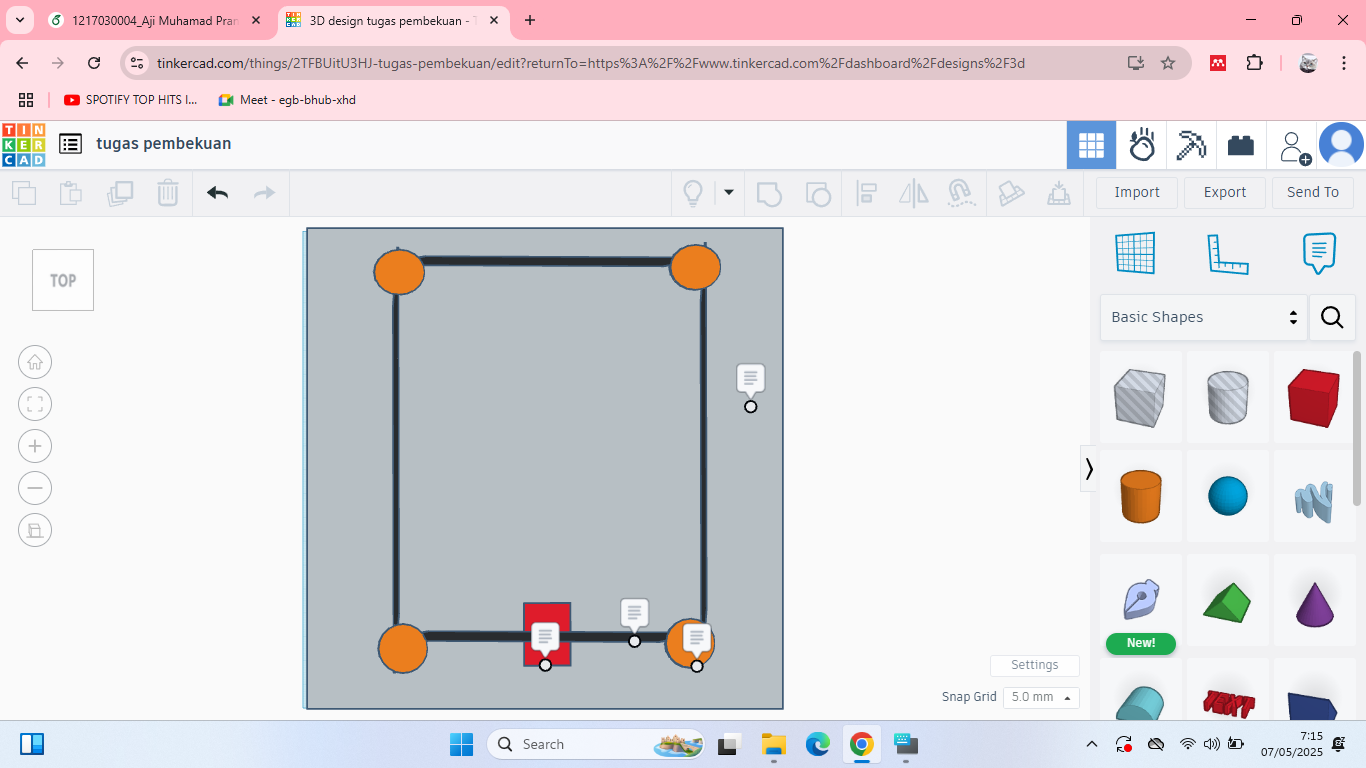
\includegraphics[width=0.5\linewidth]{images/Screenshot (5).png}
    \caption{Ilustrasi alat(tampak atas)}
    \label{fig:ilustrasi-alat-atas}
\end{figure}


\section{Kode Program}
\begin{itemize}
   \item \textbf{arduino}
   \begin{scriptsize}
    \begin{lstlisting}[language=Arduino]
       #ifdef ESP32
  #include <WiFi.h>
  #define LED_BUILTIN 2
#elif defined(ESP8266)
  #include <ESP8266WiFi.h>
#endif

#include <PubSubClient.h>
#include <ArduinoJson.h>  // Tambahkan untuk JSON yang proper

// Update these with values suitable for your network.
const char* ssid = "Aji";
const char* password = "12345678";

// **MQTT Broker Cloud**
const char* mqtt_server = "broker.hivemq.com";
const int mqtt_port = 1883;

const char* mqtt_topic = "sensor/distance";
const char* mqtt_cmd_topic = "sensor/distance/cmd";  // Tambah topik untuk command

// HC-SR04 sensor pins
#ifdef ESP32
  #define TRIG_PIN 14
  #define ECHO_PIN 27
#elif defined(ESP8266)
  #define TRIG_PIN D1
  #define ECHO_PIN D2
#endif

WiFiClient espClient;
PubSubClient client(espClient);
unsigned long lastSensorRead = 0;
unsigned long lastMqttReconnect = 0;
unsigned long lastWifiCheck = 0;
unsigned long program_start_time = 0;  // Tambah untuk timestamp
unsigned long reading_start_time = 0;  // PERBAIKAN: Tambah untuk reset waktu setiap START_READING

bool isReading = false;  // PERBAIKAN: Mulai dengan false, tunggu command dari Python
unsigned long sensorInterval = 100; // PERBAIKAN: Ubah ke 100ms untuk realtime

// Improved HC-SR04 reading dengan filtering
long readDistance() {
  digitalWrite(TRIG_PIN, LOW);
  delayMicroseconds(2);
  digitalWrite(TRIG_PIN, HIGH);
  delayMicroseconds(10);
  digitalWrite(TRIG_PIN, LOW);
  
  long duration = pulseIn(ECHO_PIN, HIGH, 30000); // Timeout 30ms
  if (duration == 0) return -1; // Timeout
  
  long distance = duration * 0.034 / 2;
  
  // Filter invalid readings
  if (distance < 2 || distance > 400) return -1;
  
  return distance;
}

void setup_wifi() {
  delay(10);
  WiFi.mode(WIFI_STA);
  WiFi.begin(ssid, password);
  
  Serial.println();
  Serial.print("Connecting to ");
  Serial.println(ssid);
  
  while (WiFi.status() != WL_CONNECTED) {
    delay(500);
    Serial.print(".");
  }
  
  randomSeed(micros());
  
  Serial.println("");
  Serial.println("WiFi connected");
  Serial.print("IP address: ");
  Serial.println(WiFi.localIP());
}

void checkWifiConnection() {
  unsigned long now = millis();
  if (now - lastWifiCheck > 10000) {
    lastWifiCheck = now;
    if (WiFi.status() != WL_CONNECTED) {
      Serial.println("WiFi disconnected, reconnecting...");
      WiFi.begin(ssid, password);
    }
  }
}

void callback(char* topic, byte* payload, unsigned int length) {
  Serial.print("Message arrived [");
  Serial.print(topic);
  Serial.print("] ");
  
  String message = "";
  for (unsigned int i = 0; i < length; i++) {
    message += (char)payload[i];
    Serial.print((char)payload[i]);
  }
  Serial.println();

  // Handle commands
  if (message == "READ_DISTANCE") {
    long distance = readDistance();
    if (distance > 0) {
      // PERBAIKAN: Kirim dengan format JSON yang proper
      JsonDocument doc;
      doc["timestamp"] = (millis() - reading_start_time) / 1000.0;  // PERBAIKAN: Gunakan reading_start_time
      doc["distance"] = distance;
      doc["device"] = "ESP8266_HCSR04";
      doc["command_response"] = true;
      
      String jsonString;
      serializeJson(doc, jsonString);
      client.publish(mqtt_topic, jsonString.c_str());
    }
  }
  else if (message == "START_READING") {
    isReading = true;
    reading_start_time = millis();  // PERBAIKAN: Reset waktu pembacaan ke 0
    Serial.println("Started continuous reading - timestamp reset to 0");
  }
  else if (message == "STOP_READING") {
    isReading = false;
    Serial.println("Stopped continuous reading");
  }
  else if (message.startsWith("INTERVAL:")) {
    // Command untuk ubah interval: "INTERVAL:100"
    int newInterval = message.substring(9).toInt();
    if (newInterval >= 50 && newInterval <= 5000) {
      sensorInterval = newInterval;
      Serial.println("Interval changed to: " + String(newInterval) + "ms");
    }
  }
  else if ((char)payload[0] == '1') {
    digitalWrite(LED_BUILTIN, LOW);
  } else {
    digitalWrite(LED_BUILTIN, HIGH);
  }
}

void reconnectMQTT() {
  unsigned long now = millis();
  if (!client.connected() && (now - lastMqttReconnect > 5000)) {
    lastMqttReconnect = now;
    Serial.print("Attempting MQTT connection...");
    
    #ifdef ESP32
      String clientId = "ESP32Client-";
    #elif defined(ESP8266)
      String clientId = "ESP8266Client-";
    #endif
    clientId += String(random(0xffff), HEX);
    
    if (client.connect(clientId.c_str())) {
      Serial.println("connected");
      
      // PERBAIKAN: Send connection message dengan JSON
      JsonDocument doc;
      doc["timestamp"] = (millis() - program_start_time) / 1000.0;
      doc["message"] = "Device connected";
      doc["device"] = clientId;
      doc["status"] = "online";
      
      String jsonString;
      serializeJson(doc, jsonString);
      client.publish(mqtt_topic, jsonString.c_str());
      
      // Subscribe ke kedua topik: data dan command
      client.subscribe(mqtt_topic);
      client.subscribe(mqtt_cmd_topic);
      Serial.println("Subscribed to data and command topics");
    } else {
      Serial.print("failed, rc=");
      Serial.print(client.state());
    }
  }
}

void setup() {
  pinMode(LED_BUILTIN, OUTPUT);
  pinMode(TRIG_PIN, OUTPUT);
  pinMode(ECHO_PIN, INPUT);
  Serial.begin(115200);
  
  // PERBAIKAN: Catat waktu mulai program
  program_start_time = millis();
  reading_start_time = millis();  // PERBAIKAN: Inisialisasi reading_start_time
  
  setup_wifi();
  
  client.setServer(mqtt_server, mqtt_port);
  client.setCallback(callback);
  
  Serial.println("System initialized");
  Serial.println("Program start time: " + String(program_start_time));
  Serial.println("Waiting for START_READING command...");  // Tambah info
}

void loop() {
  client.loop();
  
  checkWifiConnection();
  reconnectMQTT();
  
  unsigned long now = millis();
  
  // PERBAIKAN: Sensor reading dengan JSON proper dan timestamp dari reading_start_time
  if (isReading && (now - lastSensorRead >= sensorInterval)) {
    lastSensorRead = now;
    
    long distance = readDistance();
    
    if (distance > 0 && client.connected()) {
      // PERBAIKAN: Format JSON yang sesuai dengan Python, timestamp dari reading_start_time
      JsonDocument doc;
      doc["timestamp"] = (now - reading_start_time) / 1000.0;  // PERBAIKAN: Timestamp dari 0 setiap START_READING
      doc["distance"] = distance;
      doc["device"] = "ESP32_HCSR04";
      doc["uptime"] = now;
      doc["reading_time"] = (now - reading_start_time) / 1000.0;  // PERBAIKAN: Tambah info waktu pembacaan
      
      String jsonString;
      serializeJson(doc, jsonString);
      
      if (client.publish(mqtt_topic, jsonString.c_str())) {
        Serial.println("Published: " + jsonString);
      } else {
        Serial.println("Failed to publish");
      }
    } else if (distance <= 0) {
      Serial.println("Invalid distance reading");
    }
  }
  
  yield();
}
    \end{lstlisting}

    \end{scriptsize}
\end{itemize}
\begin{itemize}

   \item \textbf{python}
   \begin{scriptsize}
    \begin{lstlisting}[language=python]
        import tkinter as tk
from tkinter import filedialog, messagebox, simpledialog, ttk
from matplotlib.backends.backend_tkagg import FigureCanvasTkAgg
from matplotlib.figure import Figure
import pandas as pd
from scipy.signal import butter, filtfilt, find_peaks
import paho.mqtt.client as mqtt
import numpy as np
import json
import time
import os

# Global variables
time_data = []
distance_data = []
collecting = False
start_time = None
update_needed = False
sensor_height = 35  # cm
selected_ball_type = "Bola Bekel"  # Default ball type

# Bounce detection parameters
bounce_threshold = 15.0  # minimum bounce height (cm) - PERBAIKAN: dari 5.0 ke 15.0
min_bounce_distance = 1  # minimum distance between bounces (data points)
min_height_difference = 0.1 # minimum height difference between consecutive peaks (cm)

# MQTT Configuration - Compatible with ESP8266 and ESP32
MQTT_BROKER = "broker.hivemq.com"  # Public broker for testing
MQTT_TOPIC = "sensor/distance"     # Generic topic name
MQTT_PORT = 1883
MQTT_KEEPALIVE = 60

# Initialize MQTT client - Compatible with both ESP versions
try:
    # Try new API first (for newer paho-mqtt versions)
    client = mqtt.Client(mqtt.CallbackAPIVersion.VERSION2)
except:
    # Fallback to old API (for older paho-mqtt versions)
    client = mqtt.Client()

# GUI components
root = None
fig = None
ax = None
canvas = None
status_label = None
data_count_label = None
latest_data_label = None
data_tree = None
analysis_text = None

bola = ["Bola Bekel","Bola Tenis Meja", "Bola Tenis Lapang", 
        "Bola Plastik", "Bola Sepak Karet"]

# Global variables untuk analisis
latest_analysis_text = ""

def lowpass_filter(data, cutoff=5, fs=20, order=4):
    """Apply low-pass filter to smooth distance data"""
    min_length = max(order * 6, 20)
    if len(data) < min_length:
        return data
    
    try:
        nyq = 0.5 * fs
        normal_cutoff = cutoff / nyq
        b, a = butter(order, normal_cutoff, btype='low', analog=False)
        return filtfilt(b, a, data)
    except ValueError as e:
        print(f"Filter error: {e}")
        return data

def detect_bounces(distance_data, time_data, min_height=None, min_distance=None):
    """Detect ball bounce peaks (maximum heights) from distance data"""
    if len(distance_data) < 20:
        return [], []
    
    # Use global parameters if not provided
    if min_height is None:
        min_height = bounce_threshold
    if min_distance is None:
        min_distance = min_bounce_distance
    
    try:
        # Find peaks (maximum values) directly - no inversion needed
        peaks, properties = find_peaks(distance_data, 
                                     height=min_height,           # minimum peak height
                                     distance=min_distance,       # minimum distance between peaks
                                     prominence=3.0)              # PERBAIKAN: tingkatkan prominence dari 2.0 ke 3.0
        
        bounce_times = [time_data[p] for p in peaks if p < len(time_data)]
        bounce_distances = [distance_data[p] for p in peaks if p < len(distance_data)]
        
        # PERBAIKAN: Filter peaks berdasarkan selisih ketinggian minimal 1 cm dan trend menurun
        filtered_times = []
        filtered_distances = []
        
        if bounce_distances:
            # Tambahkan puncak pertama
            filtered_times.append(bounce_times[0])
            filtered_distances.append(bounce_distances[0])
            
            # Filter puncak selanjutnya berdasarkan selisih ketinggian dan trend menurun
            for i in range(1, len(bounce_distances)):
                height_diff = abs(bounce_distances[i] - filtered_distances[-1])
                
                # PERBAIKAN: Hanya tambahkan jika selisih ketinggian >= 1 cm DAN tinggi menurun (untuk pantulan alami)
                if height_diff >= min_height_difference and bounce_distances[i] <= filtered_distances[-1]:
                    filtered_times.append(bounce_times[i])
                    filtered_distances.append(bounce_distances[i])
                elif bounce_distances[i] > filtered_distances[-1]:
                    print(f"Puncak diabaikan: tinggi {bounce_distances[i]:.1f}cm > puncak sebelum {filtered_distances[-1]:.1f}cm (trend naik tidak wajar)")
                else:
                    print(f"Puncak diabaikan: tinggi {bounce_distances[i]:.1f}cm, selisih {height_diff:.1f}cm < {min_height_difference}cm")
        
        print(f"Detected {len(filtered_distances)} valid bounces at heights: {[round(h, 1) for h in filtered_distances]}")
        
        return filtered_times, filtered_distances
    except Exception as e:
        print(f"Bounce detection error: {e}")
        return [], []

def set_ball_type():
    """Set ball type from dropdown"""
    global selected_ball_type, update_needed
    
    # Create dialog window
    dialog = tk.Toplevel(root)
    dialog.title("Pilih Jenis Bola")
    dialog.geometry("300x200")
    dialog.resizable(False, False)
    
    # Center the dialog
    dialog.transient(root)
    dialog.grab_set()
    
    # Create frame
    frame = tk.Frame(dialog)
    frame.pack(fill=tk.BOTH, expand=True, padx=20, pady=20)
    
    tk.Label(frame, text="Pilih jenis bola yang akan diuji:", 
             font=("Arial", 11, "bold")).pack(pady=(0, 10))
    
    # Dropdown variable
    ball_var = tk.StringVar(value=selected_ball_type)
    
    # Create dropdown
    ball_dropdown = ttk.Combobox(frame, textvariable=ball_var, 
                                values=bola, state="readonly", 
                                font=("Arial", 10), width=20)
    ball_dropdown.pack(pady=(0, 20))
    
    # Button frame
    button_frame = tk.Frame(frame)
    button_frame.pack(fill=tk.X)
    
    def apply_selection():
        global selected_ball_type, update_needed
        selected_ball_type = ball_var.get()
        update_needed = True
        status_label.config(text=f"Status: Jenis bola diatur ke {selected_ball_type}", fg="blue")
        print(f"Jenis bola diubah ke: {selected_ball_type}")
        dialog.destroy()
    
    def cancel_selection():
        dialog.destroy()
    
    tk.Button(button_frame, text="Terapkan", command=apply_selection, 
             bg="lightgreen", width=10, font=("Arial", 10)).pack(side=tk.LEFT, padx=(0, 10))
    tk.Button(button_frame, text="Batal", command=cancel_selection, 
             bg="lightcoral", width=10, font=("Arial", 10)).pack(side=tk.LEFT)

def calculate_restitution_coefficient():
    """Calculate coefficient of restitution from bounce data"""
    global latest_analysis_text
    
    if len(distance_data) < 10:
        messagebox.showwarning("Peringatan", "Tidak cukup data untuk menghitung koefisien\nMinimum diperlukan: 10 titik data")
        return
    
    # PERBAIKAN: Validasi data sebelum analisis
    if len(time_data) != len(distance_data):
        messagebox.showerror("Error", f"Ketidakcocokan data:\nWaktu: {len(time_data)}\nJarak: {len(distance_data)}")
        return
    
    # PERBAIKAN: Cek adanya NaN atau Inf
    if any(np.isnan(d) or np.isinf(d) for d in distance_data):
        messagebox.showerror("Error", "Data mengandung nilai tidak valid (NaN/Inf)")
        return
    
    if any(np.isnan(t) or np.isinf(t) for t in time_data):
        messagebox.showerror("Error", "Data waktu mengandung nilai tidak valid (NaN/Inf)")
        return
    
    try:
        # Use current data without additional filtering to preserve bounce patterns
        filtered_data = distance_data
        bounce_times, bounce_distances = detect_bounces(filtered_data, time_data)
        
        if len(bounce_distances) < 2:
            messagebox.showwarning("Peringatan", 
                                 f"Perlu setidaknya 2 pantulan untuk menghitung koefisien\n"
                                 f"Saat ini terdeteksi: {len(bounce_distances)} pantulan\n"
                                 f"Coba sesuaikan pengaturan:\n"
                                 f"- Ambang pantulan (saat ini: {bounce_threshold}cm)\n"
                                 f"- Selisih tinggi minimum (saat ini: {min_height_difference}cm)\n"
                                 f"CATATAN: Sistem otomatis mengabaikan puncak yang naik (tidak wajar)")
            return
        
        # PERBAIKAN: Validasi tambahan untuk ketinggian pantulan dan trend menurun
        valid_heights = [h for h in bounce_distances if h >= bounce_threshold]
        
        # PERBAIKAN: Validasi trend menurun untuk pantulan natural
        decreasing_trend = True
        for i in range(1, len(bounce_distances)):
            if bounce_distances[i] > bounce_distances[i-1]:
                decreasing_trend = False
                break
        
        if len(valid_heights) < 2:
            messagebox.showwarning("Peringatan", 
                                 f"Tidak cukup pantulan dengan ketinggian minimal {bounce_threshold}cm\n"
                                 f"Pantulan terdeteksi: {len(bounce_distances)}\n"
                                 f"Pantulan valid (>= {bounce_threshold}cm): {len(valid_heights)}\n"
                                 f"Trend menurun: {'Ya' if decreasing_trend else 'Tidak'}\n"
                                 f"Kurangi ambang pantulan atau lakukan pengukuran ulang")
            return
        
        # Calculate coefficients between consecutive bounces
        heights = bounce_distances  # Already ball heights from ground
        coefficients = []
        bounce_intervals = []
        
        for i in range(1, len(heights)):
            if heights[i-1] >= bounce_threshold and heights[i] >= bounce_threshold:  # PERBAIKAN: Validasi kedua ketinggian
                e = np.sqrt(heights[i] / heights[i-1])
                # PERBAIKAN: Validasi koefisien
                if not (np.isnan(e) or np.isinf(e)):
                    coefficients.append(e)
                    
                    # Calculate time interval between bounces
                    time_interval = bounce_times[i] - bounce_times[i-1]
                    bounce_intervals.append(time_interval)
        
        if coefficients:
            # Statistical analysis
            avg_coefficient = np.mean(coefficients)
            std_coefficient = np.std(coefficients)
            min_coefficient = np.min(coefficients)
            max_coefficient = np.max(coefficients)
            
            # PERBAIKAN: Validasi hasil statistik
            if any(np.isnan([avg_coefficient, std_coefficient, min_coefficient, max_coefficient])):
                messagebox.showerror("Error", "Hasil perhitungan mengandung nilai tidak valid")
                return
            
            # Energy loss calculation
            energy_retention = avg_coefficient ** 2  # e² = energy ratio
            energy_loss_percent = (1 - energy_retention) * 100
            
            # Material classification based on coefficient
            if avg_coefficient >= 0.9:
                material_type = "Super Ball / Elastisitas Tinggi"
                quality = "Sangat Baik"
            elif avg_coefficient >= 0.8:
                material_type = "Bola Karet / Elastisitas Baik"
                quality = "Baik Sekali"
            elif avg_coefficient >= 0.6:
                material_type = "Bola Tenis / Elastisitas Sedang"
                quality = "Baik"
            elif avg_coefficient >= 0.4:
                material_type = "Bola Lunak / Elastisitas Rendah"
                quality = "Cukup"
            else:
                material_type = "Material Sangat Lunak / Elastisitas Buruk"
                quality = "Buruk"
            
            # Format comprehensive results untuk tampilan di frame analisis
            latest_analysis_text = f"""
{'='*60}
    ANALISIS KOEFISIEN RESTITUSI - {selected_ball_type.upper()}
{'='*60}

PENGATURAN PENGUKURAN:
  • Jenis Bola yang Diuji        : {selected_ball_type}
  • Tinggi Sensor dari Lantai    : {sensor_height:.1f} cm
  • Ambang Deteksi Pantulan      : {bounce_threshold:.1f} cm
  • Selisih Tinggi Minimum       : {min_height_difference:.1f} cm
  • Jarak Minimum Pantulan       : {min_bounce_distance} titik data
  • Total Titik Data Terkumpul   : {len(distance_data)}
  • Durasi Pengukuran            : {max(time_data):.2f} detik
  • Waktu Mulai dari             : 0.00 detik (direset setiap mulai)

{'─'*60}
HASIL DETEKSI PANTULAN:
  • Jumlah Pantulan Terdeteksi   : {len(heights)}
  • Pantulan Valid (>= {bounce_threshold}cm) : {len(valid_heights)}
  • Trend Menurun (Natural)      : {'Ya' if decreasing_trend else 'Tidak'}
  • Tinggi Pantulan (cm)         : {', '.join([f'{h:.2f}' for h in heights])}
  • Waktu Pantulan (s)           : {', '.join([f'{t:.2f}' for t in bounce_times])}
  • Interval Waktu (s)           : {', '.join([f'{t:.3f}' for t in bounce_intervals])}

{'─'*60}
PERHITUNGAN KOEFISIEN:
"""
            
            # Add individual coefficient calculations - PERBAIKAN: hanya untuk pantulan valid
            valid_pairs = 0
            for i, (e, h_before, h_after, dt) in enumerate(zip(coefficients, heights[:-1], heights[1:], bounce_intervals)):
                if h_before >= bounce_threshold and h_after >= bounce_threshold:
                    valid_pairs += 1
                    latest_analysis_text += f"  Pantulan {i+1} → {i+2} (VALID - MENURUN):\n"
                    latest_analysis_text += f"    Tinggi: {h_before:.2f} cm → {h_after:.2f} cm\n"
                    latest_analysis_text += f"    Penurunan: {h_before - h_after:.2f} cm\n"
                    latest_analysis_text += f"    Koefisien: e = √({h_after:.2f}/{h_before:.2f}) = {e:.3f}\n"
                    latest_analysis_text += f"    Interval Waktu: {dt:.3f} detik\n"
                    latest_analysis_text += f"    Energi Tersisa: {(e**2)*100:.1f}%\n\n"
                else:
                    latest_analysis_text += f"  Pantulan {i+1} → {i+2} (DIABAIKAN):\n"
                    latest_analysis_text += f"    Tinggi: {h_before:.2f} cm → {h_after:.2f} cm\n"
                    latest_analysis_text += f"    Alasan: Ketinggian < {bounce_threshold}cm\n\n"
            
            latest_analysis_text += f"""{'─'*60}
RINGKASAN STATISTIK:
  • Pasangan Pantulan Valid      : {valid_pairs} dari {len(heights)-1} total
  • Koefisien Rata-rata (e)      : {avg_coefficient:.4f}
  • Standar Deviasi              : {std_coefficient:.4f}
  • Koefisien Minimum            : {min_coefficient:.4f}
  • Koefisien Maksimum           : {max_coefficient:.4f}
  • Rentang Koefisien            : {max_coefficient - min_coefficient:.4f}

ANALISIS ENERGI:
  • Retensi Energi Rata-rata     : {energy_retention*100:.2f}%
  • Kehilangan Energi Rata-rata  : {energy_loss_percent:.2f}%
  • Tingkat Disipasi Energi      : {energy_loss_percent:.1f}% per pantulan

{'─'*60}
KLASIFIKASI MATERIAL:
  • Perkiraan Jenis Material     : {material_type}
  • Kualitas Pantulan            : {quality}
  • Rating Elastisitas           : {avg_coefficient*100:.1f}%

{'─'*60}
HASIL UNTUK {selected_ball_type.upper()}:
  • Koefisien Restitusi          : {avg_coefficient:.3f}
  • Kualitas Pantulan            : {quality}
  • Retensi Energi               : {energy_retention*100:.1f}%

{'─'*60}
PERBANDINGAN TEORITIS:
  • Tumbukan Elastis Sempurna    : e = 1.000 (100% retensi energi)
  • {selected_ball_type} Anda          : e = {avg_coefficient:.3f} ({energy_retention*100:.1f}% retensi energi)
  • Tumbukan Inelastis Sempurna  : e = 0.000 (0% retensi energi)

CATATAN FISIKA:
  • Koefisien restitusi (e) mengukur elastisitas tumbukan
  • e = 1: Tumbukan elastis sempurna (tanpa kehilangan energi)
  • e = 0: Tumbukan inelastis sempurna (kehilangan energi maksimum)
  • Material nyata umumnya memiliki 0.1 < e < 0.95
  • Koefisien tinggi berarti karakteristik pantulan bola lebih baik

PENGATURAN FILTER:
  • Tinggi minimum pantulan: {bounce_threshold}cm
  • Selisih tinggi minimum: {min_height_difference}cm
  • Filter trend menurun: AKTIF (mengabaikan puncak yang naik)
  • Filter ini memastikan hanya pantulan natural yang dihitung

{'='*60}
Analisis {selected_ball_type} selesai pada: {time.strftime('%Y-%m-%d %H:%M:%S')}
Waktu pengukuran: 0.00 - {max(time_data):.2f} detik
{'='*60}
"""
            
            # Update tampilan analisis di frame
            update_analysis_display()
            
            # Show success message
            messagebox.showinfo("Berhasil", 
                              f"Analisis koefisien restitusi {selected_ball_type} selesai!\n\n"
                              f"Pantulan valid: {valid_pairs} dari {len(heights)} (trend menurun)\n"
                              f"Koefisien rata-rata: {avg_coefficient:.3f}\n"
                              f"Kualitas pantulan: {quality}\n"
                              f"Retensi energi: {energy_retention*100:.1f}%\n"
                              f"Durasi pengukuran: {max(time_data):.2f} detik\n\n"
                              f"Hasil lengkap ditampilkan di panel Analisis Real-time")
            
        else:
            messagebox.showwarning("Peringatan", "Tidak dapat menghitung koefisien\nTidak ditemukan pasangan pantulan yang valid")
            
    except Exception as e:
        messagebox.showerror("Error", f"Error menghitung koefisien:\n{str(e)}\n\nSilakan periksa data dan pengaturan Anda")
        print(f"Calculation error details: {e}")

def on_connect(client, userdata, flags, reason_code, properties=None):
    """MQTT connection callback - compatible with ESP8266/ESP32"""
    if reason_code == 0:
        print("Terhubung ke MQTT Broker!")
        # Subscribe ke topik data untuk menerima sensor data saja
        client.subscribe(MQTT_TOPIC)
        # HAPUS subscription ke command topic untuk menghindari loop
        status_label.config(text="Status: Terhubung ke MQTT", fg="blue")
        print(f"Berlangganan ke: {MQTT_TOPIC}")
    else:
        print(f"Gagal terhubung, kode alasan {reason_code}")
        status_label.config(text="Status: Koneksi MQTT Gagal", fg="red")

def on_disconnect(client, userdata, flags, reason_code, properties=None):
    """MQTT disconnection callback"""
    print("Terputus dari MQTT Broker")
    status_label.config(text="Status: MQTT Terputus", fg="orange")

def on_message(client, userdata, msg):
    """Process incoming MQTT messages from ESP8266/ESP32"""
    global time_data, distance_data, collecting, start_time, update_needed, sensor_height
    
    # Abaikan messages dari command topic untuk menghindari loop
    if msg.topic.endswith("/cmd"):
        print(f"Mengabaikan echo perintah: {msg.payload.decode()}")
        return
    
    if not collecting:
        return
        
    try:
        # Try to parse as JSON first
        try:
            payload = json.loads(msg.payload.decode())
            print(f"Menerima JSON: {payload}")
            
            # Handle different message formats from ESP devices
            if isinstance(payload, dict):
                # Modern format with multiple fields
                t = payload.get("timestamp", payload.get("time", 0))
                d = payload.get("distance", payload.get("dist", 0))
                device = payload.get("device", payload.get("id", "ESP_Device"))
                
                # Handle status messages
                if "status" in payload or "error" in payload:
                    print(f"Pesan perangkat: {payload}")
                    return
            else:
                print(f"Format payload tidak terduga: {payload}")
                return
                
        except json.JSONDecodeError:
            # Handle simple text format: "distance:25.4"
            msg_str = msg.payload.decode().strip()
            print(f"Menerima teks: {msg_str}")
            
            if ":" in msg_str:
                parts = msg_str.split(":")
                if len(parts) == 2 and parts[0].lower() in ["distance", "dist"]:
                    try:
                        d = float(parts[1])
                        t = 0
                        device = "ESP_Text"
                    except ValueError:
                        print(f"Nilai jarak tidak valid: {parts[1]}")
                        return
                else:
                    print(f"Format teks tidak dikenal: {msg_str}")
                    return
            else:
                # Try direct number
                try:
                    d = float(msg_str)
                    t = 0
                    device = "ESP_Raw"
                except ValueError:
                    print(f"Tidak dapat mengurai pesan: {msg_str}")
                    return
        
        # PERBAIKAN: Validasi data yang lebih ketat
        if not isinstance(d, (int, float)) or d <= 0 or d > 400:
            print(f"Jarak di luar rentang: {d}")
            return
        
        if not isinstance(t, (int, float)) or t < 0:
            print(f"Timestamp tidak valid: {t}")
            if t < 0:
                t = 0  # Reset ke 0 jika negatif
        
        # Convert distance to ball height (sensor_height - distance_reading)
        ball_height = sensor_height - d
        
        # Validate ball height (should be positive for bouncing ball)
        if ball_height < 0:
            print(f"Tinggi bola negatif: {ball_height:.1f}cm (sensor terlalu rendah?)")
            return
        
        # PERBAIKAN: Handle timestamp dengan reset ke 0 setiap mulai baru
        if t > 0:
            # Use ESP provided timestamp, but adjust to start from 0
            if start_time is None:
                start_time = time.time()
            # Jika menggunakan timestamp ESP, pastikan dimulai dari 0
            current_time = float(t)
        else:
            # Generate local timestamp starting from 0
            if start_time is None:
                start_time = time.time()
            current_time = time.time() - start_time
        
        # PERBAIKAN: Validasi final sebelum menyimpan
        if np.isnan(current_time) or np.isinf(current_time) or np.isnan(ball_height) or np.isinf(ball_height):
            print(f"Data mengandung NaN atau Inf, diabaikan")
            return
        
        # Store data (now storing ball height instead of raw distance)
        time_data.append(float(current_time))
        distance_data.append(float(ball_height))
        update_needed = True
        
        # Update GUI
        data_count_label.config(text=f"Jumlah Data: {len(distance_data)}")
        latest_data_label.config(text=f"Terbaru: {ball_height:.1f}cm @ {current_time:.2f}s [{device}]")
        
        print(f"Disimpan: Waktu={current_time:.2f}s, Tinggi Bola={ball_height:.1f}cm (Mentah={d:.1f}cm), Perangkat={device}")
        
    except Exception as e:
        print(f"Error memproses pesan: {e}")

def send_mqtt_command(command):
    """Send command to ESP8266/ESP32"""
    try:
        if client.is_connected():
            # Send to command topic
            command_topic = MQTT_TOPIC + "/cmd"
            result = client.publish(command_topic, command)
            print(f"Sent command to {command_topic}: {command}")
            print(f"Publish result: {result.rc}")
            status_label.config(text=f"Status: Command sent - {command}", fg="blue")
            return True
        else:
            print("MQTT not connected")
            messagebox.showwarning("Warning", "MQTT not connected")
            return False
    except Exception as e:
        print(f"Error sending command: {e}")
        return False

def setup_mqtt():
    """Setup MQTT client with ESP8266/ESP32 compatibility"""
    try:
        # Set callbacks
        client.on_connect = on_connect
        client.on_message = on_message
        client.on_disconnect = on_disconnect
        
        print(f"Connecting to MQTT broker: {MQTT_BROKER}")
        client.connect(MQTT_BROKER, MQTT_PORT, MQTT_KEEPALIVE)
        client.loop_start()
        
    except Exception as e:
        print(f"MQTT Setup Error: {str(e)}")
        status_label.config(text="Status: MQTT Setup Failed", fg="red")

def start_collection():
    """Start data collection"""
    global collecting, start_time, update_needed
    collecting = True
    start_time = time.time()  # PERBAIKAN: Reset start_time setiap kali mulai
    update_needed = True
    status_label.config(text="Status: Mengumpulkan Data", fg="green")
    
    # PERBAIKAN: Reset data waktu agar dimulai dari 0
    if time_data:
        print("Mereset waktu ke 0 untuk pembacaan baru")
    
    # Kirim perintah ke ESP untuk mulai
    send_mqtt_command("START_READING")
    print("Pengumpulan data dimulai - waktu direset ke 0")

def stop_collection():
    """Stop data collection"""
    global collecting, update_needed
    collecting = False
    update_needed = True
    status_label.config(text="Status: Berhenti", fg="red")
    
    # Kirim perintah ke ESP untuk berhenti
    send_mqtt_command("STOP_READING")
    print("Pengumpulan data dihentikan")
    
    # Auto-calculate coefficient setelah pengumpulan data selesai
    if len(distance_data) >= 10:
        print("Menghitung koefisien restitusi otomatis...")
        root.after(1000, calculate_restitution_coefficient)  # Delay 1 detik untuk memastikan plot terupdate

def reset_data():
    """Reset all collected data"""
    global time_data, distance_data, start_time, update_needed, latest_analysis_text
    time_data.clear()
    distance_data.clear()
    start_time = None
    update_needed = True
    latest_analysis_text = ""  # PERBAIKAN: Reset hasil analisis juga
    
    data_count_label.config(text="Jumlah Data: 0")
    latest_data_label.config(text="Terbaru: -")
    status_label.config(text="Status: Data Direset", fg="blue")
    update_plot()
    update_analysis_display()  # PERBAIKAN: Update display analisis setelah reset
    print("Data dan hasil analisis telah direset.")

def update_data_table():
    """Update the data table with latest measurements"""
    global data_tree
    
    try:
        # Clear existing items
        for item in data_tree.get_children():
            data_tree.delete(item)
        
        # PERBAIKAN: Validasi data sebelum menampilkan
        if not time_data or not distance_data:
            return
        
        if len(time_data) != len(distance_data):
            print(f"Warning: Data length mismatch - time: {len(time_data)}, distance: {len(distance_data)}")
            return
        
        # Add latest 50 data points (or all if less than 50)
        start_idx = max(0, len(time_data) - 50)
        
        for i in range(start_idx, len(time_data)):
            try:
                # PERBAIKAN: Validasi setiap data point
                if i < len(time_data) and i < len(distance_data):
                    t = time_data[i]
                    d = distance_data[i]
                    
                    # Validasi tipe data
                    if isinstance(t, (int, float)) and isinstance(d, (int, float)):
                        if not (np.isnan(t) or np.isnan(d) or np.isinf(t) or np.isinf(d)):
                            raw_distance = sensor_height - d
                            
                            data_tree.insert('', 'end', values=(
                                i + 1,
                                f"{float(t):.2f}",
                                f"{float(d):.1f}",
                                f"{float(raw_distance):.1f}"
                            ))
                        else:
                            print(f"Skipping invalid data point {i}: NaN or Inf values")
                    else:
                        print(f"Skipping invalid data point {i}: wrong data type")
                        
            except Exception as e:
                print(f"Error processing data point {i}: {e}")
                continue
        
        # Scroll to bottom
        if data_tree.get_children():
            data_tree.see(data_tree.get_children()[-1])
            
    except Exception as e:
        print(f"Error updating data table: {e}")

def save_analysis_to_file():
    """Save analysis results to file"""
    global latest_analysis_text
    
    if not latest_analysis_text:
        messagebox.showwarning("Peringatan", "Tidak ada hasil analisis untuk disimpan.\nSilakan hitung koefisien restitusi terlebih dahulu.")
        return
    
    try:
        # Generate filename with ball type and timestamp
        timestamp = time.strftime("%Y%m%d_%H%M%S")
        ball_name = selected_ball_type.replace(" ", "_").replace("/", "_")  # PERBAIKAN: Hapus karakter invalid
        default_filename = f"Analisis_{ball_name}_{timestamp}.txt"
        
        file_path = filedialog.asksaveasfilename(
            defaultextension=".txt",
            filetypes=[("File Teks", "*.txt"), ("File CSV", "*.csv"), ("Semua file", "*.*")],  # PERBAIKAN: Tambah format CSV
            title="Simpan Hasil Analisis",
            initialdir=os.getcwd(),
            initialfile=default_filename
        )
        
        if file_path:
            # PERBAIKAN: Validasi dan bersihkan teks analisis
            clean_analysis_text = latest_analysis_text
            
            # Ganti karakter yang bermasalah
            clean_analysis_text = clean_analysis_text.replace('\x00', '')  # Hapus null character
            clean_analysis_text = clean_analysis_text.replace('\r\n', '\n')  # Standardize line endings
            clean_analysis_text = clean_analysis_text.replace('\r', '\n')
            
            # PERBAIKAN: Tulis dengan encoding UTF-8 dan error handling
            with open(file_path, 'w', encoding='utf-8', errors='replace') as f:
                f.write(clean_analysis_text)
            
            messagebox.showinfo("Berhasil", f"Hasil analisis {selected_ball_type} disimpan ke {file_path}")
            
    except Exception as e:
        messagebox.showerror("Error", f"Gagal menyimpan file analisis:\n{str(e)}")
        print(f"Analysis save error details: {e}")

def update_analysis_display():
    """Update the analysis display with current statistics"""
    global analysis_text, latest_analysis_text
    
    if len(distance_data) < 2:
        analysis_info = "Tidak ada data tersedia untuk analisis"
    else:
        # Check if we have detailed analysis results
        if latest_analysis_text:
            analysis_info = latest_analysis_text
        else:
            # Basic statistics jika belum ada analisis koefisien
            min_height = min(distance_data)
            max_height = max(distance_data)
            avg_height = np.mean(distance_data)
            std_height = np.std(distance_data)
            
            # Bounce detection
            bounce_times, bounce_distances = detect_bounces(distance_data, time_data)
            
            # Calculate coefficient if possible
            coefficients = []
            if len(bounce_distances) >= 2:
                for i in range(1, len(bounce_distances)):
                    if bounce_distances[i-1] > 0:
                        e = np.sqrt(bounce_distances[i] / bounce_distances[i-1])
                        coefficients.append(e)
            
            analysis_info = f"""ANALISIS REAL-TIME - {selected_ball_type.upper()}
{"="*30}

JENIS BOLA: {selected_ball_type}

STATISTIK DATA:
• Jumlah Data: {len(distance_data)}
• Durasi: {max(time_data) if time_data else 0:.1f}s
• Tinggi Min: {min_height:.1f} cm
• Tinggi Max: {max_height:.1f} cm
• Tinggi Rata-rata: {avg_height:.1f} cm
• Standar Deviasi: {std_height:.1f} cm

DETEKSI PANTULAN:
• Ambang Batas: {bounce_threshold:.1f} cm
• Pantulan Ditemukan: {len(bounce_distances)}
• Tinggi Pantulan: {[f"{h:.1f}" for h in bounce_distances[:5]]}{'...' if len(bounce_distances) > 5 else ''}

ANALISIS KOEFISIEN:
• Pasangan Valid: {len(coefficients)}
• Koefisien Rata-rata: {np.mean(coefficients):.3f if coefficients else 'N/A'}
• Retensi Energi: {np.mean(coefficients)**2*100 if coefficients else 0:.1f}%

PENGATURAN:
• Tinggi Sensor: {sensor_height:.1f} cm
• Jarak Min: {min_bounce_distance}
• Pengumpulan: {'Aktif' if collecting else 'Berhenti'}

CATATAN:
Klik "Hitung Koefisien Restitusi" untuk 
analisis lengkap dan detail perhitungan.
"""
    
    # Update analysis text widget
    analysis_text.config(state=tk.NORMAL)
    analysis_text.delete(1.0, tk.END)
    analysis_text.insert(1.0, analysis_info)
    analysis_text.config(state=tk.DISABLED)

def update_plot():
    """Update the matplotlib plot"""
    try:
        if len(time_data) == 0:
            ax.clear()
            ax.set_xlabel("Waktu (detik)")
            ax.set_ylabel("Tinggi Bola (cm)")
            ax.set_title(f"Pengukuran Tinggi {selected_ball_type} Real-time")
            ax.grid(True, alpha=0.3)
            canvas.draw_idle()
            return
        
        ax.clear()
        
        # Apply filter if enough data
        if len(distance_data) > 20:
            filtered = lowpass_filter(distance_data)
        else:
            filtered = distance_data
        
        # Plot main line
        ax.plot(time_data, filtered, 'b-', label=f"Tinggi {selected_ball_type}", linewidth=2)
        
        # Show bounces if enough data
        if len(filtered) > 20:
            bounce_times, bounce_distances = detect_bounces(filtered, time_data, 
                                                           bounce_threshold, min_bounce_distance)
            if bounce_times and bounce_distances:
                ax.plot(bounce_times, bounce_distances, "ro", label=f"Puncak Pantulan", markersize=8)
                
                # Add height annotations on peaks
                for i, (bt, bd) in enumerate(zip(bounce_times, bounce_distances)):
                    ax.annotate(f'{bd:.1f}', (bt, bd), 
                               textcoords="offset points", xytext=(0,10), ha='center',
                               fontsize=8, color='red', weight='bold')
        
        ax.set_xlabel("Waktu (detik)")
        ax.set_ylabel("Tinggi Bola (cm)")
        ax.set_title(f"Monitor Tinggi {selected_ball_type} (Sensor: {sensor_height}cm, Ambang: {bounce_threshold}cm)")
        ax.legend(loc='upper right')
        ax.grid(True, alpha=0.3)
        
        # Set axis limits
        if len(time_data) > 1:
            time_range = max(max(time_data) - min(time_data), 1)
            x_margin = time_range * 0.05
            ax.set_xlim(min(time_data) - x_margin, max(time_data) + x_margin)
        
        if len(filtered) > 1:
            dist_range = max(max(filtered) - min(filtered), 5)
            y_margin = dist_range * 0.1
            ax.set_ylim(max(0, min(filtered) - y_margin), max(filtered) + y_margin)
        
        canvas.draw_idle()
        
        # Update other displays
        update_data_table()
        update_analysis_display()
        
    except Exception as e:
        print(f"Plot update error: {e}")

def periodic_update():
    """Periodic update for real-time display"""
    global update_needed
    
    try:
        if update_needed and len(time_data) >= 0:
            update_plot()
            update_needed = False
        
        root.update_idletasks()
        
    except Exception as e:
        print(f"Periodic update error: {e}")
    
    # Schedule next update
    interval = 50 if collecting or len(time_data) > 0 else 200
    root.after(interval, periodic_update)

def set_interval():
    """Set sensor reading interval"""
    try:
        interval = simpledialog.askinteger("Atur Interval", 
                                         "Masukkan interval dalam milidetik (50-5000):",
                                         initialvalue=100, minvalue=50, maxvalue=5000)
        if interval:
            send_mqtt_command(f"INTERVAL:{interval}")
    except Exception as e:
        print(f"Error setting interval: {e}")

def set_sensor_height():
    """Set sensor height from ground"""
    global sensor_height, update_needed
    try:
        new_height = simpledialog.askfloat("Atur Tinggi Sensor", 
                                         f"Masukkan tinggi sensor dari lantai (cm):\nSaat ini: {sensor_height}cm",
                                         initialvalue=sensor_height, minvalue=10, maxvalue=200)
        if new_height:
            sensor_height = new_height
            update_needed = True
            status_label.config(text=f"Status: Tinggi sensor diatur ke {sensor_height}cm", fg="blue")
            print(f"Tinggi sensor diubah ke: {sensor_height}cm")
    except Exception as e:
        print(f"Error setting sensor height: {e}")

def set_bounce_threshold():
    """Set bounce detection threshold"""
    global bounce_threshold, update_needed
    try:
        new_threshold = simpledialog.askfloat("Atur Ambang Pantulan", 
                                            f"Masukkan tinggi minimum pantulan (cm):\nSaat ini: {bounce_threshold}cm",
                                            initialvalue=bounce_threshold, minvalue=1.0, maxvalue=50.0)
        if new_threshold:
            bounce_threshold = new_threshold
            update_needed = True
            status_label.config(text=f"Status: Ambang pantulan diatur ke {bounce_threshold}cm", fg="blue")
            print(f"Ambang pantulan diubah ke: {bounce_threshold}cm")
    except Exception as e:
        print(f"Error setting bounce threshold: {e}")

def set_min_height_difference():
    """Set minimum height difference between consecutive peaks"""
    global min_height_difference, update_needed
    try:
        new_diff = simpledialog.askfloat("Atur Selisih Tinggi Minimum", 
                                       f"Masukkan selisih tinggi minimum antar puncak (cm):\nSaat ini: {min_height_difference}cm",
                                       initialvalue=min_height_difference, minvalue=0.1, maxvalue=10.0)
        if new_diff:
            min_height_difference = new_diff
            update_needed = True
            status_label.config(text=f"Status: Selisih tinggi minimum diatur ke {min_height_difference}cm", fg="blue")
            print(f"Selisih tinggi minimum diubah ke: {min_height_difference}cm")
    except Exception as e:
        print(f"Error setting min height difference: {e}")

def set_min_bounce_distance():
    """Set minimum distance between bounces"""
    global min_bounce_distance, update_needed
    try:
        new_distance = simpledialog.askinteger("Atur Jarak Minimum Pantulan", 
                                             f"Masukkan jarak minimum antar pantulan (titik data):\nSaat ini: {min_bounce_distance}",
                                             initialvalue=min_bounce_distance, minvalue=1, maxvalue=100)
        if new_distance:
            min_bounce_distance = new_distance
            update_needed = True
            status_label.config(text=f"Status: Jarak minimum pantulan diatur ke {min_bounce_distance}", fg="blue")
            print(f"Jarak minimum pantulan diubah ke: {min_bounce_distance}")
    except Exception as e:
        print(f"Error setting min bounce distance: {e}")

def save_excel():
    """Save collected data to an Excel file."""
    if not time_data or not distance_data:
        messagebox.showwarning("Peringatan", "Tidak ada data untuk disimpan.")
        return
    
    # PERBAIKAN: Validasi data sebelum menyimpan
    if len(time_data) != len(distance_data):
        messagebox.showerror("Error", f"Ketidakcocokan jumlah data:\nWaktu: {len(time_data)}\nJarak: {len(distance_data)}")
        return
    
    try:
        # Generate filename with ball type and timestamp
        timestamp = time.strftime("%Y%m%d_%H%M%S")
        ball_name = selected_ball_type.replace(" ", "_").replace("/", "_")  # PERBAIKAN: Hapus karakter invalid
        default_filename = f"Data_{ball_name}_{timestamp}.xlsx"
        
        file_path = filedialog.asksaveasfilename(
            defaultextension=".xlsx", 
            filetypes=[("File Excel", "*.xlsx")],
            title="Simpan Data ke Excel",
            initialdir=os.getcwd(),  # PERBAIKAN: Simpan di direktori kerja saat ini
            initialfile=default_filename
        )
        
        if file_path:
            # PERBAIKAN: Validasi dan bersihkan data
            clean_time_data = []
            clean_distance_data = []
            clean_sensor_heights = []
            clean_ball_types = []
            
            for i, (t, d) in enumerate(zip(time_data, distance_data)):
                # Validasi setiap data point
                if isinstance(t, (int, float)) and isinstance(d, (int, float)):
                    if not (np.isnan(t) or np.isnan(d) or np.isinf(t) or np.isinf(d)):
                        clean_time_data.append(float(t))
                        clean_distance_data.append(float(d))
                        clean_sensor_heights.append(float(sensor_height))
                        clean_ball_types.append(str(selected_ball_type))
                    else:
                        print(f"Data point {i} diabaikan: nilai tidak valid (NaN/Inf)")
                else:
                    print(f"Data point {i} diabaikan: tipe data tidak valid")
            
            if not clean_time_data:
                messagebox.showerror("Error", "Tidak ada data valid untuk disimpan.")
                return
            
            # PERBAIKAN: Buat DataFrame dengan data yang sudah dibersihkan
            df = pd.DataFrame({
                "Waktu (detik)": clean_time_data, 
                f"Tinggi {selected_ball_type} (cm)": clean_distance_data,
                "Tinggi Sensor (cm)": clean_sensor_heights,
                "Jenis Bola": clean_ball_types
            })
            
            # PERBAIKAN: Validasi DataFrame sebelum menyimpan
            if df.empty:
                messagebox.showerror("Error", "DataFrame kosong, tidak dapat menyimpan.")
                return
            
            df.to_excel(file_path, index=False, engine='openpyxl')
            messagebox.showinfo("Berhasil", f"Data {selected_ball_type} disimpan ke {file_path}\nTotal data valid: {len(clean_time_data)}")
            
    except Exception as e:
        messagebox.showerror("Error", f"Gagal menyimpan data ke Excel:\n{str(e)}\n\nPastikan file tidak sedang dibuka di aplikasi lain.")
        print(f"Excel save error details: {e}")

def save_png():
    """Save the current plot as a PNG file."""
    try:
        # PERBAIKAN: Validasi plot sebelum menyimpan
        if fig is None or ax is None:
            messagebox.showerror("Error", "Grafik belum tersedia untuk disimpan.")
            return
        
        # Generate filename with ball type and timestamp
        timestamp = time.strftime("%Y%m%d_%H%M%S")
        ball_name = selected_ball_type.replace(" ", "_").replace("/", "_")  # PERBAIKAN: Hapus karakter invalid
        default_filename = f"Grafik_{ball_name}_{timestamp}.png"
        
        file_path = filedialog.asksaveasfilename(
            defaultextension=".png", 
            filetypes=[("File PNG", "*.png"), ("File JPG", "*.jpg"), ("File PDF", "*.pdf")],  # PERBAIKAN: Tambah format lain
            title="Simpan Grafik",
            initialdir=os.getcwd(),  # PERBAIKAN: Simpan di direktori kerja saat ini
            initialfile=default_filename
        )
        
        if file_path:
            # PERBAIKAN: Update plot sebelum menyimpan
            update_plot()
            
            # PERBAIKAN: Simpan dengan parameter yang lebih aman
            fig.savefig(file_path, 
                       dpi=300, 
                       bbox_inches='tight',
                       facecolor='white',  # PERBAIKAN: Background putih
                       edgecolor='none',   # PERBAIKAN: Tanpa border
                       format=None)        # PERBAIKAN: Auto-detect format
            
            messagebox.showinfo("Berhasil", f"Grafik {selected_ball_type} disimpan ke {file_path}")
            
    except Exception as e:
        messagebox.showerror("Error", f"Gagal menyimpan grafik:\n{str(e)}")
        print(f"PNG save error details: {e}")

def close_app():
    """Handle application close event"""
    try:
        if client.is_connected():
            client.loop_stop()
            client.disconnect()
    except Exception as e:
        print(f"Error during disconnect: {e}")
    if root is not None:
        root.destroy()

def refresh_plot_manually():
    """Manually refresh the plot."""
    update_plot()

def setup_gui():
    """Initialize GUI components with improved 2-row layout"""
    global root, fig, ax, canvas, status_label, data_count_label, latest_data_label
    global data_tree, analysis_text
    
    root = tk.Tk()
    root.title(f"Monitor Tinggi Bola HC-SR04 - {selected_ball_type}")
    root.protocol("WM_DELETE_WINDOW", close_app)
    
    # Set fullscreen
    root.state('zoomed')  # Windows fullscreen
    # Alternative for other OS: root.attributes('-zoomed', True)
    
    # Configure grid weights for responsive design
    root.grid_rowconfigure(0, weight=0)  # Title row
    root.grid_rowconfigure(1, weight=1)  # Main content row
    root.grid_rowconfigure(2, weight=0)  # Control buttons row
    root.grid_columnconfigure(0, weight=1)
    
    # ===========================================
    # BARIS 0: JUDUL UTAMA
    # ===========================================
    title_frame = tk.Frame(root, bg="navy", relief=tk.RAISED, bd=2)
    title_frame.grid(row=0, column=0, sticky="ew", padx=5, pady=5)
    
    title_label = tk.Label(title_frame, 
                          text="Analisis Koefisien Restitusi - Aji Muhamad Pranata (1217030004)",
                          font=("Arial", 16, "bold"),
                          fg="white", bg="navy", pady=10)
    title_label.pack()
    
    # ===========================================
    # BARIS 1: KONTEN UTAMA (3 KOLOM)
    # ===========================================
    main_frame = tk.Frame(root, relief=tk.RAISED, bd=1)
    main_frame.grid(row=1, column=0, sticky="nsew", padx=5, pady=5)
    
    # Configure main frame grid
    main_frame.grid_rowconfigure(0, weight=1)
    main_frame.grid_columnconfigure(0, weight=2)  # Plot gets more space
    main_frame.grid_columnconfigure(1, weight=1)  # Data table
    main_frame.grid_columnconfigure(2, weight=1)  # Analysis
    
    # -------------------------------------------
    # KOLOM 1: BAGIAN GRAFIK
    # -------------------------------------------
    plot_frame = tk.LabelFrame(main_frame, text=f"Grafik Real-time - {selected_ball_type}", font=("Arial", 12, "bold"))
    plot_frame.grid(row=0, column=0, sticky="nsew", padx=5, pady=5)
    
    # Setup matplotlib
    fig = Figure(figsize=(10, 8), dpi=100)
    ax = fig.add_subplot(111)
    ax.set_xlabel("Waktu (detik)")
    ax.set_ylabel("Tinggi Bola (cm)")
    ax.set_title(f"Pengukuran Tinggi {selected_ball_type} Real-time")
    ax.grid(True, alpha=0.3)
    
    canvas = FigureCanvasTkAgg(fig, master=plot_frame)
    canvas.get_tk_widget().pack(fill=tk.BOTH, expand=True, padx=5, pady=5)
    
    # -------------------------------------------
    # KOLOM 2: BAGIAN TABEL DATA
    # -------------------------------------------
    table_frame = tk.LabelFrame(main_frame, text="Tabel Data (50 Terakhir)", font=("Arial", 12, "bold"))
    table_frame.grid(row=0, column=1, sticky="nsew", padx=5, pady=5)
    
    # Create treeview for data table
    table_container = tk.Frame(table_frame)
    table_container.pack(fill=tk.BOTH, expand=True, padx=5, pady=5)
    
    # Scrollbars for table
    v_scrollbar = tk.Scrollbar(table_container, orient="vertical")
    h_scrollbar = tk.Scrollbar(table_container, orient="horizontal")
    
    # Data table
    columns = ('Indeks', 'Waktu (s)', 'Tinggi (cm)', 'Jarak Mentah (cm)')
    data_tree = ttk.Treeview(table_container, columns=columns, show='headings',
                            yscrollcommand=v_scrollbar.set, xscrollcommand=h_scrollbar.set)
    
    # Configure columns
    data_tree.heading('Indeks', text='#')
    data_tree.heading('Waktu (s)', text='Waktu (s)')
    data_tree.heading('Tinggi (cm)', text='Tinggi (cm)')
    data_tree.heading('Jarak Mentah (cm)', text='Jarak Mentah (cm)')
    
    data_tree.column('Indeks', width=60)
    data_tree.column('Waktu (s)', width=90)
    data_tree.column('Tinggi (cm)', width=100)
    data_tree.column('Jarak Mentah (cm)', width=120)
    
    # Pack table and scrollbars
    v_scrollbar.pack(side="right", fill="y")
    h_scrollbar.pack(side="bottom", fill="x")
    data_tree.pack(side="left", fill="both", expand=True)
    
    v_scrollbar.config(command=data_tree.yview)
    h_scrollbar.config(command=data_tree.xview)
    
    # -------------------------------------------
    # KOLOM 3: BAGIAN ANALISIS
    # -------------------------------------------
    analysis_frame = tk.LabelFrame(main_frame, text=f"Analisis Real-time & Hasil Koefisien - {selected_ball_type}", font=("Arial", 12, "bold"))
    analysis_frame.grid(row=0, column=2, sticky="nsew", padx=5, pady=5)
    
    # Analysis text widget with scrollbar
    analysis_container = tk.Frame(analysis_frame)
    analysis_container.pack(fill=tk.BOTH, expand=True, padx=5, pady=5)
    
    analysis_scrollbar = tk.Scrollbar(analysis_container)
    analysis_scrollbar.pack(side="right", fill="y")
    
    analysis_text = tk.Text(analysis_container, yscrollcommand=analysis_scrollbar.set,
                           font=("Courier", 9), wrap=tk.WORD, state=tk.DISABLED)
    analysis_text.pack(side="left", fill="both", expand=True)
    analysis_scrollbar.config(command=analysis_text.yview)
    
    # ===========================================
    # BARIS 2: TOMBOL KONTROL (BEBERAPA BARIS)
    # ===========================================
    control_frame = tk.Frame(root, relief=tk.RAISED, bd=1)
    control_frame.grid(row=2, column=0, sticky="ew", padx=5, pady=5)
    
    # Status row
    status_frame = tk.Frame(control_frame)
    status_frame.pack(fill=tk.X, padx=5, pady=2)
    
    status_label = tk.Label(status_frame, text="Status: Berhenti", font=("Arial", 14, "bold"))
    status_label.pack(side=tk.LEFT)
    
    latest_data_label = tk.Label(status_frame, text="Terbaru: -", font=("Arial", 12))
    latest_data_label.pack(side=tk.LEFT, padx=20)
    
    data_count_label = tk.Label(status_frame, text="Jumlah Data: 0", font=("Arial", 12))
    data_count_label.pack(side=tk.RIGHT)
    
    # Configuration row
    config_frame = tk.LabelFrame(control_frame, text="Konfigurasi", font=("Arial", 11, "bold"))
    config_frame.pack(fill=tk.X, padx=5, pady=3)
    
    
    tk.Button(config_frame, text=f"Jenis Bola: {selected_ball_type}", 
             command=set_ball_type, bg="lightblue", width=20, font=("Arial", 10, "bold")).pack(side=tk.LEFT, padx=3, pady=3)
    tk.Button(config_frame, text=f"Tinggi Sensor: {sensor_height}cm", 
             command=set_sensor_height, bg="lightgray", width=18, font=("Arial", 10)).pack(side=tk.LEFT, padx=3, pady=3)
    tk.Button(config_frame, text=f"Ambang Pantulan: {bounce_threshold}cm", 
             command=set_bounce_threshold, bg="lightyellow", width=20, font=("Arial", 10)).pack(side=tk.LEFT, padx=3, pady=3)
        
    tk.Button(config_frame, text=f"Selisih Tinggi Min: {min_height_difference}cm", 
             command=set_min_height_difference, bg="lightpink", width=20, font=("Arial", 10)).pack(side=tk.LEFT, padx=3, pady=3)
    tk.Button(config_frame, text=f"Jarak Min: {min_bounce_distance}", 
             command=set_min_bounce_distance, bg="lightcyan", width=15, font=("Arial", 10)).pack(side=tk.LEFT, padx=3, pady=3)
    
    # Main control row
    main_control_frame = tk.LabelFrame(control_frame, text="Kontrol Utama", font=("Arial", 11, "bold"))
    main_control_frame.pack(fill=tk.X, padx=5, pady=3)
    
    tk.Button(main_control_frame, text="Mulai Pengumpulan", command=start_collection, 
             bg="lightgreen", width=15, font=("Arial", 10, "bold")).pack(side=tk.LEFT, padx=3, pady=3)
    tk.Button(main_control_frame, text="Hentikan Pengumpulan", command=stop_collection, 
             bg="lightcoral", width=18, font=("Arial", 10, "bold")).pack(side=tk.LEFT, padx=3, pady=3)
    tk.Button(main_control_frame, text="Reset Data", command=reset_data, 
             bg="lightyellow", width=12, font=("Arial", 10)).pack(side=tk.LEFT, padx=3, pady=3)
    tk.Button(main_control_frame, text="Refresh Grafik", command=refresh_plot_manually, 
             bg="lightcyan", width=12, font=("Arial", 10)).pack(side=tk.LEFT, padx=3, pady=3)
    
    # Analysis and export row
    analysis_control_frame = tk.LabelFrame(control_frame, text="Analisis & Ekspor", font=("Arial", 11, "bold"))
    analysis_control_frame.pack(fill=tk.X, padx=5, pady=3)
    
    tk.Button(analysis_control_frame, text="Hitung Koefisien Restitusi", command=calculate_restitution_coefficient, 
             bg="orange", width=20, font=("Arial", 10, "bold")).pack(side=tk.LEFT, padx=3, pady=3)
    tk.Button(analysis_control_frame, text="Simpan Hasil Analisis", command=save_analysis_to_file, 
             bg="lightgreen", width=15, font=("Arial", 10)).pack(side=tk.LEFT, padx=3, pady=3)
    tk.Button(analysis_control_frame, text="Simpan Data (Excel)", command=save_excel, 
             bg="lightblue", width=15, font=("Arial", 10)).pack(side=tk.LEFT, padx=3, pady=3)
    tk.Button(analysis_control_frame, text="Simpan Grafik (PNG)", command=save_png, 
             bg="lightblue", width=15, font=("Arial", 10)).pack(side=tk.LEFT, padx=3, pady=3)
    
    # ESP control row
    esp_control_frame = tk.LabelFrame(control_frame, text="Kontrol ESP8266/ESP32", font=("Arial", 11, "bold"))
    esp_control_frame.pack(fill=tk.X, padx=5, pady=3)
    
    tk.Button(esp_control_frame, text="Mulai Pembacaan ESP", command=lambda: send_mqtt_command("START_READING"), 
             bg="lightgreen", width=18, font=("Arial", 10)).pack(side=tk.LEFT, padx=3, pady=3)
    tk.Button(esp_control_frame, text="Hentikan Pembacaan ESP", command=lambda: send_mqtt_command("STOP_READING"), 
             bg="lightcoral", width=20, font=("Arial", 10)).pack(side=tk.LEFT, padx=3, pady=3)
    tk.Button(esp_control_frame, text="Minta Jarak", command=lambda: send_mqtt_command("READ_DISTANCE"), 
             bg="lightyellow", width=12, font=("Arial", 10)).pack(side=tk.LEFT, padx=3, pady=3)
    tk.Button(esp_control_frame, text="Atur Interval", command=set_interval, 
             bg="lightcyan", width=12, font=("Arial", 10)).pack(side=tk.LEFT, padx=3, pady=3)
    
    # Exit button
    tk.Button(esp_control_frame, text="Keluar Aplikasi", command=close_app, 
             bg="lightgray", width=15, font=("Arial", 10, "bold")).pack(side=tk.RIGHT, padx=3, pady=3)
    
    # Initialize displays
    update_analysis_display()

def main():
    """Main application entry point"""
    print("=== Monitor Tinggi Bola HC-SR04 ===")
    print("Kompatibel dengan ESP8266 dan ESP32")
    print(f"MQTT Broker: {MQTT_BROKER}")
    print(f"MQTT Topic: {MQTT_TOPIC}")
    print(f"Tinggi Sensor: {sensor_height}cm")
    print("=====================================")
    
    # Setup GUI
    setup_gui()
    
    # Setup MQTT
    setup_mqtt()
    
    # Start periodic updates
    root.after(100, periodic_update)
    
    print("Aplikasi dimulai!")
    print("- Klik 'Mulai' untuk memulai pengumpulan data")
    print("- Atur tinggi sensor sebelum pengukuran")
    print("- Perangkat ESP harus mempublikasikan ke topik:", MQTT_TOPIC)
    
    # Start GUI main loop
    root.mainloop()

if __name__ == "__main__":
    main()
    \end{lstlisting}
    \end{scriptsize}
\end{itemize}
 
% \documentclass[a4paper,12pt]{report}

% \usepackage{geometry}

% \geometry{
%   left=3cm,
%   right=2cm,
%   top=3cm,
%   bottom=2cm,
%   headheight=14pt,
%   headsep=20pt,
%   footskip=30pt
% }

% \usepackage{titlesec}
% \usepackage{tabularray}
% \usepackage{graphicx}
% \usepackage{longtable}

% \begin{document}

% % Lampiran
% \appendix

% \renewcommand{\chaptername}{LAMPIRAN}
% \titleformat{\chapter}[display]
% {\normalfont\huge \bfseries \centering}
% {\chaptername~\thechapter}
% {12pt}
% {}

% % Section, Figure, and Table Numbering (e.g., 1.1, 1.1.1)
% \renewcommand{\thesection}{\arabic{chapter}.\arabic{section}}
% \renewcommand{\thesubsection}{\thesection.\arabic{subsection}}
% \renewcommand{\thesubsubsection}{\thesubsection.\arabic{subsubsection}}
% \renewcommand{\thefigure}{\arabic{chapter}.\arabic{figure}}
% \renewcommand{\thetable}{\arabic{chapter}.\arabic{table}}

% \setcounter{chapter}{4}
% \setcounter{page}{93}

\chapter{Tabel dan Grafik Setiap Percobaan}
\section{Bola Bekel}
\subsection{Tabel Percobaan}

\begin{longtable}[htbp]{|c|c|c|}
\caption{Data Bola Bekel 1} \\
\hline
Waktu (detik) & Tinggi Bola Bekel (cm) & Tinggi Sensor (cm) \\ \hline
\endfirsthead
\caption[]{Data Bola Bekel 1} \\
\hline
Waktu (detik) & Tinggi Bola Bekel (cm) & Tinggi Sensor (cm) \\ \hline
\endhead
\multicolumn{3}{r}{Continued on next page} \\
\endfoot
\endlastfoot
0.733918 & 22 & 35 \\ \hline
0.100000 & 28 & 35 \\ \hline
0.200000 & 31 & 35 \\ \hline
0.300000 & 33 & 35 \\ \hline
0.400000 & 33 & 35 \\ \hline
0.500000 & 30 & 35 \\ \hline
0.600000 & 22 & 35 \\ \hline
0.700000 & 14 & 35 \\ \hline
1.400000 & 5 & 35 \\ \hline
1.500000 & 12 & 35 \\ \hline
1.600000 & 19 & 35 \\ \hline
1.700000 & 25 & 35 \\ \hline
1.808000 & 29 & 35 \\ \hline
1.908000 & 31 & 35 \\ \hline
2.008000 & 31 & 35 \\ \hline
2.108000 & 28 & 35 \\ \hline
2.208000 & 24 & 35 \\ \hline
2.308000 & 16 & 35 \\ \hline
2.408000 & 6 & 35 \\ \hline
3.114000 & 5 & 35 \\ \hline
3.214000 & 11 & 35 \\ \hline
3.314000 & 17 & 35 \\ \hline
3.414000 & 22 & 35 \\ \hline
3.514000 & 24 & 35 \\ \hline
3.614000 & 25 & 35 \\ \hline
3.714000 & 25 & 35 \\ \hline
3.814000 & 24 & 35 \\ \hline
3.914000 & 18 & 35 \\ \hline
4.021000 & 8 & 35 \\ \hline
4.721000 & 0 & 35 \\ \hline
4.821000 & 6 & 35 \\ \hline
4.921000 & 11 & 35 \\ \hline
5.021000 & 16 & 35 \\ \hline
5.121000 & 19 & 35 \\ \hline
5.221000 & 19 & 35 \\ \hline
5.321000 & 19 & 35 \\ \hline
5.421000 & 17 & 35 \\ \hline
5.521000 & 10 & 35 \\ \hline
5.621000 & 4 & 35 \\ \hline
6.525000 & 5 & 35 \\ \hline
6.625000 & 8 & 35 \\ \hline
6.725000 & 10 & 35 \\ \hline
6.825000 & 11 & 35 \\ \hline
6.925000 & 11 & 35 \\ \hline
7.025000 & 7 & 35 \\ \hline
\end{longtable}

\begin{longtable}[htbp]{|c|c|c|}
\caption{Data Bola Bekel 2} \\
\hline
Waktu (detik) & Tinggi Bola Bekel (cm) & Tinggi Sensor (cm) \\ \hline
\endfirsthead
\caption[]{Data Bola Bekel 2} \\
\hline
Waktu (detik) & Tinggi Bola Bekel (cm) & Tinggi Sensor (cm) \\ \hline
\endhead
\multicolumn{3}{r}{Continued on next page} \\
\endfoot
\endlastfoot
0.200000 & 10 & 35 \\ \hline
0.300000 & 6 & 35 \\ \hline
0.400000 & 10 & 35 \\ \hline
0.500000 & 19 & 35 \\ \hline
0.600000 & 27 & 35 \\ \hline
0.700000 & 32 & 35 \\ \hline
0.800000 & 33 & 35 \\ \hline
0.900000 & 33 & 35 \\ \hline
1.800000 & 29 & 35 \\ \hline
1.900000 & 31 & 35 \\ \hline
2.000000 & 21 & 35 \\ \hline
2.100000 & 6 & 35 \\ \hline
3.402000 & 4 & 35 \\ \hline
3.502000 & 12 & 35 \\ \hline
3.602000 & 19 & 35 \\ \hline
3.702000 & 25 & 35 \\ \hline
3.802000 & 28 & 35 \\ \hline
3.902000 & 29 & 35 \\ \hline
4.002000 & 28 & 35 \\ \hline
4.102000 & 24 & 35 \\ \hline
4.402000 & 0 & 35 \\ \hline
5.711000 & 8 & 35 \\ \hline
5.811000 & 16 & 35 \\ \hline
5.911000 & 20 & 35 \\ \hline
6.011000 & 25 & 35 \\ \hline
6.121000 & 26 & 35 \\ \hline
6.221000 & 26 & 35 \\ \hline
6.331000 & 23 & 35 \\ \hline
6.431000 & 17 & 35 \\ \hline
6.531000 & 8 & 35 \\ \hline
7.752000 & 5 & 35 \\ \hline
7.852000 & 14 & 35 \\ \hline
7.952000 & 19 & 35 \\ \hline
8.052000 & 23 & 35 \\ \hline
8.152000 & 23 & 35 \\ \hline
8.252000 & 23 & 35 \\ \hline
8.352000 & 19 & 35 \\ \hline
8.452000 & 14 & 35 \\ \hline
8.552000 & 6 & 35 \\ \hline
9.753000 & 1 & 35 \\ \hline
9.853000 & 9 & 35 \\ \hline
9.953000 & 17 & 35 \\ \hline
10.053000 & 20 & 35 \\ \hline
10.153000 & 20 & 35 \\ \hline
10.253000 & 19 & 35 \\ \hline
10.353000 & 13 & 35 \\ \hline
10.453000 & 6 & 35 \\ \hline
11.653000 & 4 & 35 \\ \hline
11.753000 & 10 & 35 \\ \hline
\end{longtable}

\begin{longtable}[htbp]{|c|c|c|}
\caption{Data Bola Bekel 3} \\
\hline
Waktu (detik) & Tinggi Bola Bekel (cm) & Tinggi Sensor (cm) \\ \hline
\endfirsthead
\caption[]{Data Bola Bekel 3} \\
\hline
Waktu (detik) & Tinggi Bola Bekel (cm) & Tinggi Sensor (cm) \\ \hline
\endhead
\multicolumn{3}{r}{Continued on next page} \\
\endfoot
\endlastfoot
0.646137 & 20 & 35 \\ \hline
0.100000 & 9 & 35 \\ \hline
1.300000 & 0 & 35 \\ \hline
1.400000 & 10 & 35 \\ \hline
1.500000 & 18 & 35 \\ \hline
1.600000 & 23 & 35 \\ \hline
1.700000 & 29 & 35 \\ \hline
1.800000 & 32 & 35 \\ \hline
1.900000 & 31 & 35 \\ \hline
2.000000 & 28 & 35 \\ \hline
2.100000 & 21 & 35 \\ \hline
2.200000 & 11 & 35 \\ \hline
3.410000 & 2 & 35 \\ \hline
3.510000 & 11 & 35 \\ \hline
3.610000 & 19 & 35 \\ \hline
3.710000 & 24 & 35 \\ \hline
3.810000 & 28 & 35 \\ \hline
3.910000 & 29 & 35 \\ \hline
4.010000 & 30 & 35 \\ \hline
4.110000 & 26 & 35 \\ \hline
4.210000 & 18 & 35 \\ \hline
4.310000 & 6 & 35 \\ \hline
5.612000 & 0 & 35 \\ \hline
5.712000 & 8 & 35 \\ \hline
5.812000 & 15 & 35 \\ \hline
5.912000 & 20 & 35 \\ \hline
6.012000 & 25 & 35 \\ \hline
6.112000 & 27 & 35 \\ \hline
6.212000 & 28 & 35 \\ \hline
6.312000 & 25 & 35 \\ \hline
6.412000 & 19 & 35 \\ \hline
6.512000 & 12 & 35 \\ \hline
6.612000 & 0 & 35 \\ \hline
7.812000 & 4 & 35 \\ \hline
7.912000 & 13 & 35 \\ \hline
8.012000 & 19 & 35 \\ \hline
8.112000 & 20 & 35 \\ \hline
8.212000 & 21 & 35 \\ \hline
8.321000 & 19 & 35 \\ \hline
8.421000 & 13 & 35 \\ \hline
8.526000 & 4 & 35 \\ \hline
9.726000 & 2 & 35 \\ \hline
9.826000 & 9 & 35 \\ \hline
9.936000 & 17 & 35 \\ \hline
10.036000 & 19 & 35 \\ \hline
10.136000 & 19 & 35 \\ \hline
10.236000 & 19 & 35 \\ \hline
10.336000 & 16 & 35 \\ \hline
10.436000 & 9 & 35 \\ \hline
10.536000 & 0 & 35 \\ \hline
\end{longtable}

\begin{longtable}[htbp]{|c|c|c|}
\caption{Data Bola Bekel 4} \\
\hline
Waktu (detik) & Tinggi Bola Bekel (cm) & Tinggi Sensor (cm) \\ \hline
\endfirsthead
\caption[]{Data Bola Bekel 4} \\
\hline
Waktu (detik) & Tinggi Bola Bekel (cm) & Tinggi Sensor (cm) \\ \hline
\endhead
\multicolumn{3}{r}{Continued on next page} \\
\endfoot
\endlastfoot
3.750000 & 11 & 35 \\ \hline
3.850000 & 10 & 35 \\ \hline
3.950000 & 29 & 35 \\ \hline
4.050000 & 31 & 35 \\ \hline
4.150000 & 33 & 35 \\ \hline
4.250000 & 32 & 35 \\ \hline
4.350000 & 32 & 35 \\ \hline
4.450000 & 31 & 35 \\ \hline
4.550000 & 32 & 35 \\ \hline
4.650000 & 32 & 35 \\ \hline
4.750000 & 31 & 35 \\ \hline
4.850000 & 32 & 35 \\ \hline
4.950000 & 32 & 35 \\ \hline
5.050000 & 32 & 35 \\ \hline
5.150000 & 31 & 35 \\ \hline
5.250000 & 27 & 35 \\ \hline
5.350000 & 32 & 35 \\ \hline
5.450000 & 24 & 35 \\ \hline
5.550000 & 14 & 35 \\ \hline
6.750000 & 4 & 35 \\ \hline
6.850000 & 11 & 35 \\ \hline
6.950000 & 19 & 35 \\ \hline
7.050000 & 24 & 35 \\ \hline
7.150000 & 29 & 35 \\ \hline
7.250000 & 31 & 35 \\ \hline
7.350000 & 32 & 35 \\ \hline
7.450000 & 31 & 35 \\ \hline
7.550000 & 27 & 35 \\ \hline
7.650000 & 19 & 35 \\ \hline
7.750000 & 10 & 35 \\ \hline
8.950000 & 5 & 35 \\ \hline
9.050000 & 14 & 35 \\ \hline
9.150000 & 19 & 35 \\ \hline
9.250000 & 24 & 35 \\ \hline
9.350000 & 26 & 35 \\ \hline
9.450000 & 25 & 35 \\ \hline
9.550000 & 21 & 35 \\ \hline
9.650000 & 14 & 35 \\ \hline
9.750000 & 5 & 35 \\ \hline
10.950000 & 5 & 35 \\ \hline
11.050000 & 13 & 35 \\ \hline
11.150000 & 20 & 35 \\ \hline
11.250000 & 25 & 35 \\ \hline
11.350000 & 26 & 35 \\ \hline
11.450000 & 23 & 35 \\ \hline
11.550000 & 19 & 35 \\ \hline
11.650000 & 11 & 35 \\ \hline
11.750000 & 2 & 35 \\ \hline
12.950000 & 5 & 35 \\ \hline
13.050000 & 13 & 35 \\ \hline
13.150000 & 19 & 35 \\ \hline
13.250000 & 20 & 35 \\ \hline
13.350000 & 19 & 35 \\ \hline
13.450000 & 13 & 35 \\ \hline
13.550000 & 6 & 35 \\ \hline
14.650000 & 0 & 35 \\ \hline
14.750000 & 6 & 35 \\ \hline
14.850000 & 10 & 35 \\ \hline
14.950000 & 11 & 35 \\ \hline
15.050000 & 12 & 35 \\ \hline
15.151000 & 6 & 35 \\ \hline
\end{longtable}

\begin{longtable}[htbp]{|c|c|c|}
\caption{Data Bola Bekel 5} \\
\hline
Waktu (detik) & Tinggi Bola Bekel (cm) & Tinggi Sensor (cm) \\ \hline
\endfirsthead
\caption[]{Data Bola Bekel 5} \\
\hline
Waktu (detik) & Tinggi Bola Bekel (cm) & Tinggi Sensor (cm) \\ \hline
\endhead
\multicolumn{3}{r}{Continued on next page} \\
\endfoot
\endlastfoot
0.100000 & 33 & 35 \\ \hline
0.200000 & 26 & 35 \\ \hline
0.300000 & 15 & 35 \\ \hline
0.400000 & 3 & 35 \\ \hline
1.600000 & 14 & 35 \\ \hline
1.700000 & 24 & 35 \\ \hline
1.800000 & 30 & 35 \\ \hline
1.900000 & 33 & 35 \\ \hline
2.000000 & 32 & 35 \\ \hline
2.100000 & 31 & 35 \\ \hline
2.200000 & 24 & 35 \\ \hline
2.300000 & 15 & 35 \\ \hline
2.400000 & 3 & 35 \\ \hline
3.605000 & 8 & 35 \\ \hline
3.705000 & 15 & 35 \\ \hline
3.805000 & 20 & 35 \\ \hline
3.905000 & 26 & 35 \\ \hline
4.005000 & 29 & 35 \\ \hline
4.105000 & 30 & 35 \\ \hline
4.205000 & 26 & 35 \\ \hline
4.305000 & 21 & 35 \\ \hline
4.405000 & 12 & 35 \\ \hline
5.805000 & 0 & 35 \\ \hline
5.905000 & 8 & 35 \\ \hline
6.005000 & 16 & 35 \\ \hline
6.105000 & 20 & 35 \\ \hline
6.205000 & 25 & 35 \\ \hline
6.305000 & 25 & 35 \\ \hline
6.405000 & 24 & 35 \\ \hline
6.505000 & 19 & 35 \\ \hline
6.605000 & 10 & 35 \\ \hline
7.905000 & 4 & 35 \\ \hline
8.005000 & 11 & 35 \\ \hline
8.105000 & 16 & 35 \\ \hline
8.205000 & 19 & 35 \\ \hline
8.306000 & 19 & 35 \\ \hline
8.406000 & 17 & 35 \\ \hline
8.511000 & 12 & 35 \\ \hline
10.119000 & 4 & 35 \\ \hline
10.219000 & 9 & 35 \\ \hline
10.319000 & 12 & 35 \\ \hline
10.419000 & 9 & 35 \\ \hline
10.519000 & 6 & 35 \\ \hline
\end{longtable}

\begin{longtable}[htbp]{|c|c|c|}
\caption{Data Bola Bekel 6} \\
\hline
Waktu (detik) & Tinggi Bola Bekel (cm) & Tinggi Sensor (cm) \\ \hline
\endfirsthead
\caption[]{Data Bola Bekel 6} \\
\hline
Waktu (detik) & Tinggi Bola Bekel (cm) & Tinggi Sensor (cm) \\ \hline
\endhead
\multicolumn{3}{r}{Continued on next page} \\
\endfoot
\endlastfoot
0.793083 & 5 & 35 \\ \hline
0.300000 & 3 & 35 \\ \hline
0.400000 & 13 & 35 \\ \hline
0.500000 & 23 & 35 \\ \hline
0.600000 & 29 & 35 \\ \hline
0.700000 & 32 & 35 \\ \hline
0.800000 & 33 & 35 \\ \hline
0.900000 & 33 & 35 \\ \hline
1.000000 & 28 & 35 \\ \hline
1.100000 & 19 & 35 \\ \hline
1.200000 & 10 & 35 \\ \hline
2.300000 & 4 & 35 \\ \hline
2.400000 & 12 & 35 \\ \hline
2.500000 & 20 & 35 \\ \hline
2.600000 & 27 & 35 \\ \hline
2.700000 & 31 & 35 \\ \hline
2.800000 & 33 & 35 \\ \hline
2.900000 & 33 & 35 \\ \hline
3.000000 & 28 & 35 \\ \hline
3.100000 & 21 & 35 \\ \hline
3.200000 & 10 & 35 \\ \hline
3.300000 & 4 & 35 \\ \hline
4.303000 & 6 & 35 \\ \hline
4.403000 & 15 & 35 \\ \hline
4.503000 & 22 & 35 \\ \hline
4.603000 & 27 & 35 \\ \hline
4.703000 & 28 & 35 \\ \hline
4.803000 & 28 & 35 \\ \hline
4.903000 & 24 & 35 \\ \hline
5.003000 & 17 & 35 \\ \hline
5.103000 & 8 & 35 \\ \hline
6.103000 & 0 & 35 \\ \hline
6.203000 & 7 & 35 \\ \hline
6.303000 & 13 & 35 \\ \hline
6.403000 & 20 & 35 \\ \hline
6.503000 & 24 & 35 \\ \hline
6.603000 & 25 & 35 \\ \hline
6.703000 & 25 & 35 \\ \hline
6.803000 & 20 & 35 \\ \hline
6.903000 & 12 & 35 \\ \hline
7.003000 & 3 & 35 \\ \hline
8.105000 & 6 & 35 \\ \hline
8.205000 & 13 & 35 \\ \hline
8.305000 & 19 & 35 \\ \hline
8.405000 & 19 & 35 \\ \hline
8.505000 & 18 & 35 \\ \hline
8.605000 & 13 & 35 \\ \hline
8.705000 & 6 & 35 \\ \hline
9.505000 & 13 & 35 \\ \hline
10.907000 & 19 & 35 \\ \hline
\end{longtable}

\begin{longtable}[htbp]{|c|c|c|}
\caption{Data Bola Bekel 7} \\
\hline
Waktu (detik) & Tinggi Bola Bekel (cm) & Tinggi Sensor (cm) \\ \hline
\endfirsthead
\caption[]{Data Bola Bekel 7} \\
\hline
Waktu (detik) & Tinggi Bola Bekel (cm) & Tinggi Sensor (cm) \\ \hline
\endhead
\multicolumn{3}{r}{Continued on next page} \\
\endfoot
\endlastfoot
0.600000 & 7 & 35 \\ \hline
0.700000 & 19 & 35 \\ \hline
0.800000 & 28 & 35 \\ \hline
0.900000 & 32 & 35 \\ \hline
1.100000 & 33 & 35 \\ \hline
1.200000 & 29 & 35 \\ \hline
1.300000 & 21 & 35 \\ \hline
1.400000 & 19 & 35 \\ \hline
2.602000 & 6 & 35 \\ \hline
2.702000 & 15 & 35 \\ \hline
2.802000 & 22 & 35 \\ \hline
2.902000 & 29 & 35 \\ \hline
3.002000 & 32 & 35 \\ \hline
3.102000 & 32 & 35 \\ \hline
3.202000 & 31 & 35 \\ \hline
3.302000 & 27 & 35 \\ \hline
3.402000 & 20 & 35 \\ \hline
3.502000 & 11 & 35 \\ \hline
3.602000 & 1 & 35 \\ \hline
4.705000 & 0 & 35 \\ \hline
4.808000 & 8 & 35 \\ \hline
4.908000 & 17 & 35 \\ \hline
5.008000 & 23 & 35 \\ \hline
5.108000 & 27 & 35 \\ \hline
5.208000 & 31 & 35 \\ \hline
5.308000 & 31 & 35 \\ \hline
5.408000 & 29 & 35 \\ \hline
5.508000 & 24 & 35 \\ \hline
5.608000 & 18 & 35 \\ \hline
5.708000 & 8 & 35 \\ \hline
6.711000 & 0 & 35 \\ \hline
6.811000 & 6 & 35 \\ \hline
6.911000 & 15 & 35 \\ \hline
7.011000 & 21 & 35 \\ \hline
7.111000 & 24 & 35 \\ \hline
7.211000 & 25 & 35 \\ \hline
7.311000 & 24 & 35 \\ \hline
7.411000 & 20 & 35 \\ \hline
7.511000 & 13 & 35 \\ \hline
7.611000 & 5 & 35 \\ \hline
8.311000 & 19 & 35 \\ \hline
8.611000 & 0 & 35 \\ \hline
8.711000 & 8 & 35 \\ \hline
8.811000 & 15 & 35 \\ \hline
8.911000 & 20 & 35 \\ \hline
9.015000 & 22 & 35 \\ \hline
9.115000 & 20 & 35 \\ \hline
9.215000 & 15 & 35 \\ \hline
9.315000 & 8 & 35 \\ \hline
9.415000 & 0 & 35 \\ \hline
\end{longtable}

\begin{longtable}[htbp]{|c|c|c|}
\caption{Data Bola Bekel 8} \\
\hline
Waktu (detik) & Tinggi Bola Bekel (cm) & Tinggi Sensor (cm) \\ \hline
\endfirsthead
\caption[]{Data Bola Bekel 8} \\
\hline
Waktu (detik) & Tinggi Bola Bekel (cm) & Tinggi Sensor (cm) \\ \hline
\endhead
\multicolumn{3}{r}{Continued on next page} \\
\endfoot
\endlastfoot
0.200000 & 9 & 35 \\ \hline
0.300000 & 19 & 35 \\ \hline
0.400000 & 27 & 35 \\ \hline
0.500000 & 32 & 35 \\ \hline
0.600000 & 33 & 35 \\ \hline
0.700000 & 32 & 35 \\ \hline
0.800000 & 33 & 35 \\ \hline
0.900000 & 30 & 35 \\ \hline
1.000000 & 20 & 35 \\ \hline
1.100000 & 8 & 35 \\ \hline
2.106000 & 0 & 35 \\ \hline
2.206000 & 10 & 35 \\ \hline
2.306000 & 19 & 35 \\ \hline
2.406000 & 27 & 35 \\ \hline
2.506000 & 30 & 35 \\ \hline
2.606000 & 33 & 35 \\ \hline
2.706000 & 32 & 35 \\ \hline
2.810000 & 29 & 35 \\ \hline
2.910000 & 22 & 35 \\ \hline
3.010000 & 12 & 35 \\ \hline
3.110000 & 3 & 35 \\ \hline
3.713000 & 3 & 35 \\ \hline
4.013000 & 2 & 35 \\ \hline
4.113000 & 9 & 35 \\ \hline
4.213000 & 19 & 35 \\ \hline
4.315000 & 26 & 35 \\ \hline
4.415000 & 30 & 35 \\ \hline
4.515000 & 31 & 35 \\ \hline
4.615000 & 30 & 35 \\ \hline
4.715000 & 25 & 35 \\ \hline
4.815000 & 17 & 35 \\ \hline
4.915000 & 7 & 35 \\ \hline
5.915000 & 6 & 35 \\ \hline
6.015000 & 17 & 35 \\ \hline
6.115000 & 22 & 35 \\ \hline
6.219000 & 27 & 35 \\ \hline
6.319000 & 28 & 35 \\ \hline
6.419000 & 26 & 35 \\ \hline
6.519000 & 20 & 35 \\ \hline
6.619000 & 12 & 35 \\ \hline
6.719000 & 2 & 35 \\ \hline
7.621000 & 1 & 35 \\ \hline
7.721000 & 9 & 35 \\ \hline
7.821000 & 17 & 35 \\ \hline
7.921000 & 21 & 35 \\ \hline
8.021000 & 23 & 35 \\ \hline
8.121000 & 22 & 35 \\ \hline
8.221000 & 17 & 35 \\ \hline
8.321000 & 8 & 35 \\ \hline
\end{longtable}

\begin{longtable}[htbp]{|c|c|c|}
\caption{Data Bola Bekel 9} \\
\hline
Waktu (detik) & Tinggi Bola Bekel (cm) & Tinggi Sensor (cm) \\ \hline
\endfirsthead
\caption[]{Data Bola Bekel 9} \\
\hline
Waktu (detik) & Tinggi Bola Bekel (cm) & Tinggi Sensor (cm) \\ \hline
\endhead
\multicolumn{3}{r}{Continued on next page} \\
\endfoot
\endlastfoot
1.404000 & 6 & 35 \\ \hline
1.504000 & 16 & 35 \\ \hline
1.604000 & 23 & 35 \\ \hline
1.704000 & 30 & 35 \\ \hline
1.804000 & 32 & 35 \\ \hline
1.904000 & 33 & 35 \\ \hline
2.004000 & 33 & 35 \\ \hline
2.104000 & 30 & 35 \\ \hline
2.204000 & 20 & 35 \\ \hline
2.304000 & 13 & 35 \\ \hline
3.404000 & 1 & 35 \\ \hline
3.504000 & 10 & 35 \\ \hline
3.604000 & 19 & 35 \\ \hline
3.708000 & 25 & 35 \\ \hline
3.808000 & 30 & 35 \\ \hline
3.908000 & 31 & 35 \\ \hline
4.008000 & 32 & 35 \\ \hline
4.108000 & 30 & 35 \\ \hline
4.208000 & 25 & 35 \\ \hline
4.308000 & 18 & 35 \\ \hline
4.408000 & 6 & 35 \\ \hline
5.515000 & 7 & 35 \\ \hline
5.615000 & 16 & 35 \\ \hline
5.715000 & 21 & 35 \\ \hline
5.815000 & 25 & 35 \\ \hline
5.924000 & 28 & 35 \\ \hline
6.024000 & 27 & 35 \\ \hline
6.131000 & 24 & 35 \\ \hline
6.231000 & 19 & 35 \\ \hline
6.331000 & 12 & 35 \\ \hline
6.431000 & 2 & 35 \\ \hline
7.431000 & 1 & 35 \\ \hline
7.531000 & 12 & 35 \\ \hline
7.631000 & 18 & 35 \\ \hline
7.731000 & 20 & 35 \\ \hline
7.831000 & 23 & 35 \\ \hline
7.931000 & 23 & 35 \\ \hline
8.031000 & 19 & 35 \\ \hline
8.131000 & 13 & 35 \\ \hline
8.231000 & 7 & 35 \\ \hline
9.335000 & 4 & 35 \\ \hline
9.435000 & 11 & 35 \\ \hline
9.535000 & 16 & 35 \\ \hline
9.635000 & 19 & 35 \\ \hline
9.735000 & 20 & 35 \\ \hline
9.835000 & 20 & 35 \\ \hline
9.935000 & 17 & 35 \\ \hline
10.035000 & 11 & 35 \\ \hline
11.440000 & 0 & 35 \\ \hline
11.540000 & 4 & 35 \\ \hline
11.640000 & 8 & 35 \\ \hline
11.740000 & 11 & 35 \\ \hline
11.840000 & 13 & 35 \\ \hline
11.940000 & 13 & 35 \\ \hline
12.040000 & 10 & 35 \\ \hline
12.140000 & 6 & 35 \\ \hline
12.240000 & 0 & 35 \\ \hline
\end{longtable}

\begin{longtable}[htbp]{|c|c|c|}
\caption{Data Bola Bekel 10} \\
\hline
Waktu (detik) & Tinggi Bola Bekel (cm) & Tinggi Sensor (cm) \\ \hline
\endfirsthead
\caption[]{Data Bola Bekel 10} \\
\hline
Waktu (detik) & Tinggi Bola Bekel (cm) & Tinggi Sensor (cm) \\ \hline
\endhead
\multicolumn{3}{r}{Continued on next page} \\
\endfoot
\endlastfoot
0.600000 & 9 & 35 \\ \hline
0.700000 & 19 & 35 \\ \hline
0.800000 & 27 & 35 \\ \hline
0.900000 & 32 & 35 \\ \hline
1.009000 & 33 & 35 \\ \hline
1.109000 & 33 & 35 \\ \hline
1.209000 & 29 & 35 \\ \hline
1.309000 & 22 & 35 \\ \hline
1.409000 & 11 & 35 \\ \hline
2.409000 & 2 & 35 \\ \hline
2.509000 & 12 & 35 \\ \hline
2.609000 & 19 & 35 \\ \hline
2.709000 & 27 & 35 \\ \hline
2.809000 & 31 & 35 \\ \hline
2.915000 & 32 & 35 \\ \hline
3.015000 & 30 & 35 \\ \hline
3.115000 & 26 & 35 \\ \hline
3.215000 & 18 & 35 \\ \hline
3.315000 & 9 & 35 \\ \hline
4.315000 & 9 & 35 \\ \hline
4.415000 & 17 & 35 \\ \hline
4.515000 & 22 & 35 \\ \hline
4.615000 & 26 & 35 \\ \hline
4.715000 & 27 & 35 \\ \hline
4.815000 & 25 & 35 \\ \hline
4.915000 & 19 & 35 \\ \hline
5.015000 & 13 & 35 \\ \hline
5.115000 & 5 & 35 \\ \hline
6.115000 & 4 & 35 \\ \hline
6.215000 & 12 & 35 \\ \hline
6.315000 & 18 & 35 \\ \hline
6.415000 & 23 & 35 \\ \hline
6.515000 & 25 & 35 \\ \hline
6.615000 & 24 & 35 \\ \hline
6.715000 & 20 & 35 \\ \hline
6.815000 & 13 & 35 \\ \hline
6.924000 & 6 & 35 \\ \hline
7.827000 & 0 & 35 \\ \hline
7.927000 & 8 & 35 \\ \hline
8.027000 & 13 & 35 \\ \hline
8.127000 & 17 & 35 \\ \hline
8.227000 & 17 & 35 \\ \hline
8.327000 & 12 & 35 \\ \hline
8.427000 & 4 & 35 \\ \hline
\end{longtable}

\begin{longtable}[htbp]{|c|c|c|}
\caption{Data Bola Bekel 11} \\
\hline
Waktu (detik) & Tinggi Bola Bekel (cm) & Tinggi Sensor (cm) \\ \hline
\endfirsthead
\caption[]{Data Bola Bekel 11} \\
\hline
Waktu (detik) & Tinggi Bola Bekel (cm) & Tinggi Sensor (cm) \\ \hline
\endhead
\multicolumn{3}{r}{Continued on next page} \\
\endfoot
\endlastfoot
1.405000 & 3 & 35 \\ \hline
1.505000 & 13 & 35 \\ \hline
1.605000 & 19 & 35 \\ \hline
1.705000 & 26 & 35 \\ \hline
1.814000 & 32 & 35 \\ \hline
1.914000 & 33 & 35 \\ \hline
2.014000 & 32 & 35 \\ \hline
2.114000 & 30 & 35 \\ \hline
2.214000 & 25 & 35 \\ \hline
2.314000 & 17 & 35 \\ \hline
2.414000 & 7 & 35 \\ \hline
3.422000 & 5 & 35 \\ \hline
3.522000 & 15 & 35 \\ \hline
3.625000 & 20 & 35 \\ \hline
3.725000 & 26 & 35 \\ \hline
3.825000 & 30 & 35 \\ \hline
3.925000 & 32 & 35 \\ \hline
4.025000 & 32 & 35 \\ \hline
4.125000 & 30 & 35 \\ \hline
4.225000 & 23 & 35 \\ \hline
4.325000 & 17 & 35 \\ \hline
4.425000 & 6 & 35 \\ \hline
5.325000 & 2 & 35 \\ \hline
5.425000 & 10 & 35 \\ \hline
5.525000 & 18 & 35 \\ \hline
5.627000 & 21 & 35 \\ \hline
5.727000 & 26 & 35 \\ \hline
5.827000 & 28 & 35 \\ \hline
5.927000 & 27 & 35 \\ \hline
6.027000 & 27 & 35 \\ \hline
6.127000 & 28 & 35 \\ \hline
6.227000 & 29 & 35 \\ \hline
6.327000 & 29 & 35 \\ \hline
6.436000 & 28 & 35 \\ \hline
6.536000 & 24 & 35 \\ \hline
6.636000 & 18 & 35 \\ \hline
6.745000 & 8 & 35 \\ \hline
7.653000 & 2 & 35 \\ \hline
7.753000 & 10 & 35 \\ \hline
7.953000 & 22 & 35 \\ \hline
8.053000 & 25 & 35 \\ \hline
8.153000 & 25 & 35 \\ \hline
8.253000 & 23 & 35 \\ \hline
8.362000 & 19 & 35 \\ \hline
8.462000 & 13 & 35 \\ \hline
8.572000 & 4 & 35 \\ \hline
9.472000 & 4 & 35 \\ \hline
9.572000 & 10 & 35 \\ \hline
9.672000 & 15 & 35 \\ \hline
9.772000 & 19 & 35 \\ \hline
9.872000 & 20 & 35 \\ \hline
9.978000 & 20 & 35 \\ \hline
10.078000 & 19 & 35 \\ \hline
10.178000 & 16 & 35 \\ \hline
10.278000 & 9 & 35 \\ \hline
10.378000 & 2 & 35 \\ \hline
\end{longtable}

\begin{longtable}[htbp]{|c|c|c|}
\caption{Data Bola Bekel 12} \\
\hline
Waktu (detik) & Tinggi Bola Bekel (cm) & Tinggi Sensor (cm) \\ \hline
\endfirsthead
\caption[]{Data Bola Bekel 12} \\
\hline
Waktu (detik) & Tinggi Bola Bekel (cm) & Tinggi Sensor (cm) \\ \hline
\endhead
\multicolumn{3}{r}{Continued on next page} \\
\endfoot
\endlastfoot
0.085000 & 2 & 35 \\ \hline
0.185000 & 12 & 35 \\ \hline
0.285000 & 19 & 35 \\ \hline
0.385000 & 27 & 35 \\ \hline
0.485000 & 31 & 35 \\ \hline
0.585000 & 32 & 35 \\ \hline
0.685000 & 32 & 35 \\ \hline
0.785000 & 32 & 35 \\ \hline
0.885000 & 32 & 35 \\ \hline
0.986000 & 28 & 35 \\ \hline
1.086000 & 33 & 35 \\ \hline
1.187000 & 32 & 35 \\ \hline
1.287000 & 29 & 35 \\ \hline
1.387000 & 21 & 35 \\ \hline
1.487000 & 12 & 35 \\ \hline
1.587000 & 0 & 35 \\ \hline
2.497000 & 6 & 35 \\ \hline
2.597000 & 14 & 35 \\ \hline
2.697000 & 21 & 35 \\ \hline
2.797000 & 27 & 35 \\ \hline
2.897000 & 30 & 35 \\ \hline
2.997000 & 32 & 35 \\ \hline
3.097000 & 32 & 35 \\ \hline
3.197000 & 31 & 35 \\ \hline
3.297000 & 30 & 35 \\ \hline
3.397000 & 26 & 35 \\ \hline
3.497000 & 19 & 35 \\ \hline
3.597000 & 8 & 35 \\ \hline
3.697000 & 0 & 35 \\ \hline
4.597000 & 5 & 35 \\ \hline
4.697000 & 13 & 35 \\ \hline
4.797000 & 19 & 35 \\ \hline
4.897000 & 26 & 35 \\ \hline
4.997000 & 29 & 35 \\ \hline
5.097000 & 30 & 35 \\ \hline
5.197000 & 31 & 35 \\ \hline
5.297000 & 30 & 35 \\ \hline
5.397000 & 31 & 35 \\ \hline
5.497000 & 28 & 35 \\ \hline
5.597000 & 23 & 35 \\ \hline
5.697000 & 14 & 35 \\ \hline
5.797000 & 6 & 35 \\ \hline
6.697000 & 2 & 35 \\ \hline
6.900000 & 18 & 35 \\ \hline
7.001000 & 23 & 35 \\ \hline
7.111000 & 26 & 35 \\ \hline
7.211000 & 28 & 35 \\ \hline
7.311000 & 29 & 35 \\ \hline
7.411000 & 26 & 35 \\ \hline
7.511000 & 23 & 35 \\ \hline
7.611000 & 14 & 35 \\ \hline
7.711000 & 5 & 35 \\ \hline
8.611000 & 0 & 35 \\ \hline
8.712000 & 6 & 35 \\ \hline
8.812000 & 15 & 35 \\ \hline
8.912000 & 19 & 35 \\ \hline
9.012000 & 23 & 35 \\ \hline
9.112000 & 25 & 35 \\ \hline
9.212000 & 25 & 35 \\ \hline
9.312000 & 19 & 35 \\ \hline
9.412000 & 13 & 35 \\ \hline
9.512000 & 6 & 35 \\ \hline
10.412000 & 4 & 35 \\ \hline
10.512000 & 9 & 35 \\ \hline
10.612000 & 13 & 35 \\ \hline
10.712000 & 15 & 35 \\ \hline
10.812000 & 18 & 35 \\ \hline
10.912000 & 18 & 35 \\ \hline
11.012000 & 16 & 35 \\ \hline
11.112000 & 13 & 35 \\ \hline
11.212000 & 6 & 35 \\ \hline
11.312000 & 1 & 35 \\ \hline
\end{longtable}

\begin{longtable}[htbp]{|c|c|c|}
\caption{Data Bola Bekel 13} \\
\hline
Waktu (detik) & Tinggi Bola Bekel (cm) & Tinggi Sensor (cm) \\ \hline
\endfirsthead
\caption[]{Data Bola Bekel 13} \\
\hline
Waktu (detik) & Tinggi Bola Bekel (cm) & Tinggi Sensor (cm) \\ \hline
\endhead
\multicolumn{3}{r}{Continued on next page} \\
\endfoot
\endlastfoot
0.575000 & 1 & 35 \\ \hline
0.100000 & 12 & 35 \\ \hline
0.200000 & 20 & 35 \\ \hline
0.300000 & 26 & 35 \\ \hline
0.400000 & 31 & 35 \\ \hline
0.500000 & 32 & 35 \\ \hline
0.600000 & 32 & 35 \\ \hline
0.700000 & 33 & 35 \\ \hline
0.800000 & 30 & 35 \\ \hline
0.900000 & 23 & 35 \\ \hline
1.000000 & 13 & 35 \\ \hline
1.100000 & 3 & 35 \\ \hline
2.102000 & 5 & 35 \\ \hline
2.202000 & 13 & 35 \\ \hline
2.302000 & 20 & 35 \\ \hline
2.402000 & 25 & 35 \\ \hline
2.502000 & 30 & 35 \\ \hline
2.602000 & 32 & 35 \\ \hline
2.702000 & 32 & 35 \\ \hline
2.802000 & 31 & 35 \\ \hline
2.902000 & 25 & 35 \\ \hline
3.002000 & 19 & 35 \\ \hline
3.102000 & 10 & 35 \\ \hline
3.202000 & 1 & 35 \\ \hline
4.102000 & 4 & 35 \\ \hline
4.202000 & 12 & 35 \\ \hline
4.302000 & 19 & 35 \\ \hline
4.402000 & 25 & 35 \\ \hline
4.502000 & 29 & 35 \\ \hline
4.602000 & 30 & 35 \\ \hline
4.702000 & 27 & 35 \\ \hline
4.802000 & 23 & 35 \\ \hline
4.902000 & 17 & 35 \\ \hline
5.002000 & 8 & 35 \\ \hline
6.002000 & 1 & 35 \\ \hline
6.102000 & 9 & 35 \\ \hline
6.202000 & 19 & 35 \\ \hline
6.302000 & 24 & 35 \\ \hline
6.402000 & 26 & 35 \\ \hline
6.502000 & 26 & 35 \\ \hline
6.602000 & 21 & 35 \\ \hline
6.702000 & 14 & 35 \\ \hline
6.802000 & 6 & 35 \\ \hline
7.802000 & 3 & 35 \\ \hline
8.002000 & 18 & 35 \\ \hline
8.102000 & 22 & 35 \\ \hline
8.202000 & 25 & 35 \\ \hline
8.302000 & 25 & 35 \\ \hline
8.402000 & 24 & 35 \\ \hline
8.502000 & 19 & 35 \\ \hline
8.602000 & 11 & 35 \\ \hline
8.702000 & 2 & 35 \\ \hline
9.702000 & 4 & 35 \\ \hline
9.802000 & 6 & 35 \\ \hline
9.902000 & 5 & 35 \\ \hline
10.002000 & 0 & 35 \\ \hline
\end{longtable}

\begin{longtable}[htbp]{|c|c|c|}
\caption{Data Bola Bekel 14} \\
\hline
Waktu (detik) & Tinggi Bola Bekel (cm) & Tinggi Sensor (cm) \\ \hline
\endfirsthead
\caption[]{Data Bola Bekel 14} \\
\hline
Waktu (detik) & Tinggi Bola Bekel (cm) & Tinggi Sensor (cm) \\ \hline
\endhead
\multicolumn{3}{r}{Continued on next page} \\
\endfoot
\endlastfoot
2.806000 & 6 & 35 \\ \hline
2.906000 & 18 & 35 \\ \hline
3.006000 & 25 & 35 \\ \hline
3.106000 & 30 & 35 \\ \hline
3.206000 & 33 & 35 \\ \hline
3.306000 & 33 & 35 \\ \hline
3.406000 & 33 & 35 \\ \hline
3.506000 & 32 & 35 \\ \hline
3.606000 & 29 & 35 \\ \hline
3.706000 & 21 & 35 \\ \hline
3.806000 & 12 & 35 \\ \hline
3.906000 & 2 & 35 \\ \hline
4.906000 & 6 & 35 \\ \hline
5.006000 & 13 & 35 \\ \hline
5.106000 & 22 & 35 \\ \hline
5.206000 & 27 & 35 \\ \hline
5.306000 & 32 & 35 \\ \hline
5.406000 & 33 & 35 \\ \hline
5.506000 & 32 & 35 \\ \hline
5.606000 & 29 & 35 \\ \hline
5.706000 & 24 & 35 \\ \hline
5.806000 & 15 & 35 \\ \hline
5.906000 & 5 & 35 \\ \hline
6.806000 & 1 & 35 \\ \hline
6.906000 & 8 & 35 \\ \hline
7.006000 & 14 & 35 \\ \hline
7.106000 & 21 & 35 \\ \hline
7.206000 & 26 & 35 \\ \hline
7.306000 & 29 & 35 \\ \hline
7.406000 & 30 & 35 \\ \hline
7.506000 & 28 & 35 \\ \hline
7.606000 & 25 & 35 \\ \hline
7.706000 & 17 & 35 \\ \hline
7.806000 & 8 & 35 \\ \hline
8.806000 & 4 & 35 \\ \hline
8.906000 & 12 & 35 \\ \hline
9.006000 & 19 & 35 \\ \hline
9.106000 & 22 & 35 \\ \hline
9.206000 & 26 & 35 \\ \hline
9.306000 & 27 & 35 \\ \hline
9.406000 & 26 & 35 \\ \hline
9.506000 & 23 & 35 \\ \hline
9.606000 & 16 & 35 \\ \hline
9.706000 & 7 & 35 \\ \hline
10.812000 & 5 & 35 \\ \hline
10.914000 & 12 & 35 \\ \hline
11.014000 & 19 & 35 \\ \hline
11.114000 & 22 & 35 \\ \hline
11.214000 & 25 & 35 \\ \hline
11.314000 & 23 & 35 \\ \hline
11.414000 & 20 & 35 \\ \hline
11.514000 & 14 & 35 \\ \hline
11.614000 & 5 & 35 \\ \hline
12.914000 & 3 & 35 \\ \hline
13.014000 & 8 & 35 \\ \hline
13.114000 & 13 & 35 \\ \hline
13.222000 & 17 & 35 \\ \hline
13.322000 & 19 & 35 \\ \hline
13.422000 & 19 & 35 \\ \hline
13.522000 & 22 & 35 \\ \hline
13.622000 & 21 & 35 \\ \hline
13.722000 & 19 & 35 \\ \hline
13.822000 & 12 & 35 \\ \hline
13.925000 & 4 & 35 \\ \hline
\end{longtable}

\begin{longtable}[htbp]{|c|c|c|}
\caption{Data Bola Bekel 15} \\
\hline
Waktu (detik) & Tinggi Bola Bekel (cm) & Tinggi Sensor (cm) \\ \hline
\endfirsthead
\caption[]{Data Bola Bekel 15} \\
\hline
Waktu (detik) & Tinggi Bola Bekel (cm) & Tinggi Sensor (cm) \\ \hline
\endhead
\multicolumn{3}{r}{Continued on next page} \\
\endfoot
\endlastfoot
0.601000 & 1 & 35 \\ \hline
0.701000 & 13 & 35 \\ \hline
0.801000 & 21 & 35 \\ \hline
0.901000 & 27 & 35 \\ \hline
1.001000 & 31 & 35 \\ \hline
1.101000 & 32 & 35 \\ \hline
1.201000 & 24 & 35 \\ \hline
1.301000 & 32 & 35 \\ \hline
1.401000 & 33 & 35 \\ \hline
1.501000 & 31 & 35 \\ \hline
1.601000 & 24 & 35 \\ \hline
1.701000 & 16 & 35 \\ \hline
1.801000 & 8 & 35 \\ \hline
2.813000 & 2 & 35 \\ \hline
2.913000 & 10 & 35 \\ \hline
3.020000 & 18 & 35 \\ \hline
3.120000 & 23 & 35 \\ \hline
3.220000 & 29 & 35 \\ \hline
3.320000 & 32 & 35 \\ \hline
3.420000 & 32 & 35 \\ \hline
3.520000 & 32 & 35 \\ \hline
3.620000 & 28 & 35 \\ \hline
3.720000 & 23 & 35 \\ \hline
3.820000 & 14 & 35 \\ \hline
3.920000 & 5 & 35 \\ \hline
4.820000 & 5 & 35 \\ \hline
4.920000 & 12 & 35 \\ \hline
5.020000 & 19 & 35 \\ \hline
5.120000 & 23 & 35 \\ \hline
5.220000 & 28 & 35 \\ \hline
5.321000 & 30 & 35 \\ \hline
5.421000 & 30 & 35 \\ \hline
5.521000 & 27 & 35 \\ \hline
5.621000 & 22 & 35 \\ \hline
5.721000 & 14 & 35 \\ \hline
5.821000 & 4 & 35 \\ \hline
6.721000 & 5 & 35 \\ \hline
6.821000 & 13 & 35 \\ \hline
6.921000 & 19 & 35 \\ \hline
7.021000 & 25 & 35 \\ \hline
7.121000 & 28 & 35 \\ \hline
7.221000 & 28 & 35 \\ \hline
7.321000 & 26 & 35 \\ \hline
7.421000 & 21 & 35 \\ \hline
7.521000 & 13 & 35 \\ \hline
7.627000 & 4 & 35 \\ \hline
8.534000 & 6 & 35 \\ \hline
8.634000 & 11 & 35 \\ \hline
8.734000 & 18 & 35 \\ \hline
8.834000 & 21 & 35 \\ \hline
8.934000 & 25 & 35 \\ \hline
9.034000 & 25 & 35 \\ \hline
9.134000 & 24 & 35 \\ \hline
9.234000 & 19 & 35 \\ \hline
9.434000 & 4 & 35 \\ \hline
10.434000 & 0 & 35 \\ \hline
10.534000 & 5 & 35 \\ \hline
10.634000 & 10 & 35 \\ \hline
10.734000 & 15 & 35 \\ \hline
10.835000 & 18 & 35 \\ \hline
10.935000 & 18 & 35 \\ \hline
11.042000 & 16 & 35 \\ \hline
11.142000 & 10 & 35 \\ \hline
11.242000 & 5 & 35 \\ \hline
\end{longtable}

\begin{longtable}[htbp]{|c|c|c|}
\caption{Data Bola Bekel 16} \\
\hline
Waktu (detik) & Tinggi Bola Bekel (cm) & Tinggi Sensor (cm) \\ \hline
\endfirsthead
\caption[]{Data Bola Bekel 16} \\
\hline
Waktu (detik) & Tinggi Bola Bekel (cm) & Tinggi Sensor (cm) \\ \hline
\endhead
\multicolumn{3}{r}{Continued on next page} \\
\endfoot
\endlastfoot
0.800000 & 8 & 35 \\ \hline
0.900000 & 16 & 35 \\ \hline
1.000000 & 24 & 35 \\ \hline
1.100000 & 29 & 35 \\ \hline
1.200000 & 32 & 35 \\ \hline
1.300000 & 32 & 35 \\ \hline
1.400000 & 31 & 35 \\ \hline
1.500000 & 26 & 35 \\ \hline
1.600000 & 17 & 35 \\ \hline
1.702000 & 8 & 35 \\ \hline
2.902000 & 8 & 35 \\ \hline
3.002000 & 17 & 35 \\ \hline
3.102000 & 25 & 35 \\ \hline
3.202000 & 30 & 35 \\ \hline
3.302000 & 33 & 35 \\ \hline
3.402000 & 32 & 35 \\ \hline
3.502000 & 28 & 35 \\ \hline
3.602000 & 21 & 35 \\ \hline
3.702000 & 10 & 35 \\ \hline
3.802000 & 0 & 35 \\ \hline
4.702000 & 3 & 35 \\ \hline
4.806000 & 12 & 35 \\ \hline
4.906000 & 19 & 35 \\ \hline
5.006000 & 24 & 35 \\ \hline
5.106000 & 30 & 35 \\ \hline
5.206000 & 32 & 35 \\ \hline
5.306000 & 29 & 35 \\ \hline
5.406000 & 23 & 35 \\ \hline
5.506000 & 16 & 35 \\ \hline
5.606000 & 7 & 35 \\ \hline
6.506000 & 6 & 35 \\ \hline
6.606000 & 13 & 35 \\ \hline
6.706000 & 20 & 35 \\ \hline
6.806000 & 26 & 35 \\ \hline
6.906000 & 30 & 35 \\ \hline
7.006000 & 30 & 35 \\ \hline
7.106000 & 27 & 35 \\ \hline
7.206000 & 23 & 35 \\ \hline
7.306000 & 15 & 35 \\ \hline
7.406000 & 6 & 35 \\ \hline
8.306000 & 6 & 35 \\ \hline
8.406000 & 13 & 35 \\ \hline
8.506000 & 20 & 35 \\ \hline
8.606000 & 24 & 35 \\ \hline
8.706000 & 27 & 35 \\ \hline
8.806000 & 28 & 35 \\ \hline
8.906000 & 25 & 35 \\ \hline
9.006000 & 20 & 35 \\ \hline
9.206000 & 3 & 35 \\ \hline
10.106000 & 5 & 35 \\ \hline
10.206000 & 12 & 35 \\ \hline
10.306000 & 19 & 35 \\ \hline
10.406000 & 22 & 35 \\ \hline
10.506000 & 26 & 35 \\ \hline
10.606000 & 25 & 35 \\ \hline
10.706000 & 22 & 35 \\ \hline
10.806000 & 16 & 35 \\ \hline
10.906000 & 8 & 35 \\ \hline
\end{longtable}

\begin{longtable}[htbp]{|c|c|c|}
\caption{Data Bola Bekel 17} \\
\hline
Waktu (detik) & Tinggi Bola Bekel (cm) & Tinggi Sensor (cm) \\ \hline
\endfirsthead
\caption[]{Data Bola Bekel 17} \\
\hline
Waktu (detik) & Tinggi Bola Bekel (cm) & Tinggi Sensor (cm) \\ \hline
\endhead
\multicolumn{3}{r}{Continued on next page} \\
\endfoot
\endlastfoot
0.501000 & 4 & 35 \\ \hline
0.601000 & 16 & 35 \\ \hline
0.701000 & 24 & 35 \\ \hline
0.801000 & 30 & 35 \\ \hline
0.901000 & 33 & 35 \\ \hline
1.001000 & 33 & 35 \\ \hline
1.101000 & 29 & 35 \\ \hline
1.201000 & 22 & 35 \\ \hline
1.301000 & 10 & 35 \\ \hline
2.101000 & 1 & 35 \\ \hline
2.201000 & 10 & 35 \\ \hline
2.301000 & 20 & 35 \\ \hline
2.401000 & 26 & 35 \\ \hline
2.501000 & 31 & 35 \\ \hline
2.601000 & 31 & 35 \\ \hline
2.701000 & 28 & 35 \\ \hline
2.801000 & 22 & 35 \\ \hline
2.901000 & 12 & 35 \\ \hline
3.802000 & 3 & 35 \\ \hline
3.902000 & 13 & 35 \\ \hline
4.002000 & 21 & 35 \\ \hline
4.102000 & 26 & 35 \\ \hline
4.203000 & 29 & 35 \\ \hline
4.303000 & 27 & 35 \\ \hline
4.403000 & 24 & 35 \\ \hline
4.503000 & 15 & 35 \\ \hline
4.603000 & 6 & 35 \\ \hline
5.503000 & 6 & 35 \\ \hline
5.603000 & 14 & 35 \\ \hline
5.703000 & 21 & 35 \\ \hline
5.803000 & 23 & 35 \\ \hline
5.903000 & 21 & 35 \\ \hline
6.003000 & 18 & 35 \\ \hline
6.103000 & 11 & 35 \\ \hline
7.103000 & 6 & 35 \\ \hline
7.203000 & 13 & 35 \\ \hline
7.303000 & 19 & 35 \\ \hline
7.403000 & 19 & 35 \\ \hline
7.503000 & 17 & 35 \\ \hline
7.603000 & 11 & 35 \\ \hline
7.703000 & 4 & 35 \\ \hline
\end{longtable}

\begin{longtable}[htbp]{|c|c|c|}
\caption{Data Bola Bekel 18} \\
\hline
Waktu (detik) & Tinggi Bola Bekel (cm) & Tinggi Sensor (cm) \\ \hline
\endfirsthead
\caption[]{Data Bola Bekel 18} \\
\hline
Waktu (detik) & Tinggi Bola Bekel (cm) & Tinggi Sensor (cm) \\ \hline
\endhead
\multicolumn{3}{r}{Continued on next page} \\
\endfoot
\endlastfoot
0.500000 & 16 & 35 \\ \hline
0.600000 & 23 & 35 \\ \hline
0.700000 & 30 & 35 \\ \hline
0.800000 & 32 & 35 \\ \hline
0.900000 & 32 & 35 \\ \hline
1.000000 & 32 & 35 \\ \hline
1.100000 & 26 & 35 \\ \hline
1.200000 & 17 & 35 \\ \hline
1.300000 & 7 & 35 \\ \hline
2.308000 & 1 & 35 \\ \hline
2.408000 & 9 & 35 \\ \hline
2.508000 & 17 & 35 \\ \hline
2.608000 & 25 & 35 \\ \hline
2.708000 & 29 & 35 \\ \hline
2.808000 & 32 & 35 \\ \hline
2.908000 & 32 & 35 \\ \hline
3.008000 & 30 & 35 \\ \hline
3.108000 & 22 & 35 \\ \hline
3.208000 & 14 & 35 \\ \hline
3.308000 & 3 & 35 \\ \hline
4.208000 & 0 & 35 \\ \hline
4.308000 & 10 & 35 \\ \hline
4.408000 & 18 & 35 \\ \hline
4.508000 & 23 & 35 \\ \hline
4.608000 & 27 & 35 \\ \hline
4.708000 & 29 & 35 \\ \hline
4.808000 & 29 & 35 \\ \hline
4.908000 & 26 & 35 \\ \hline
5.008000 & 19 & 35 \\ \hline
5.108000 & 6 & 35 \\ \hline
6.008000 & 2 & 35 \\ \hline
6.108000 & 9 & 35 \\ \hline
6.208000 & 18 & 35 \\ \hline
6.308000 & 24 & 35 \\ \hline
6.408000 & 27 & 35 \\ \hline
6.508000 & 29 & 35 \\ \hline
6.608000 & 27 & 35 \\ \hline
6.708000 & 23 & 35 \\ \hline
6.808000 & 15 & 35 \\ \hline
6.908000 & 6 & 35 \\ \hline
7.818000 & 6 & 35 \\ \hline
7.918000 & 13 & 35 \\ \hline
8.018000 & 20 & 35 \\ \hline
8.122000 & 24 & 35 \\ \hline
8.222000 & 27 & 35 \\ \hline
8.322000 & 25 & 35 \\ \hline
8.422000 & 19 & 35 \\ \hline
8.522000 & 11 & 35 \\ \hline
8.622000 & 4 & 35 \\ \hline
9.630000 & 5 & 35 \\ \hline
9.730000 & 13 & 35 \\ \hline
9.830000 & 19 & 35 \\ \hline
9.930000 & 22 & 35 \\ \hline
10.030000 & 23 & 35 \\ \hline
10.130000 & 20 & 35 \\ \hline
10.230000 & 16 & 35 \\ \hline
10.330000 & 10 & 35 \\ \hline
10.430000 & 3 & 35 \\ \hline
11.530000 & 3 & 35 \\ \hline
11.630000 & 8 & 35 \\ \hline
11.730000 & 13 & 35 \\ \hline
11.830000 & 15 & 35 \\ \hline
11.930000 & 16 & 35 \\ \hline
12.030000 & 16 & 35 \\ \hline
12.130000 & 13 & 35 \\ \hline
12.230000 & 6 & 35 \\ \hline
\end{longtable}

\begin{longtable}[htbp]{|c|c|c|}
\caption{Data Bola Bekel 19} \\
\hline
Waktu (detik) & Tinggi Bola Bekel (cm) & Tinggi Sensor (cm) \\ \hline
\endfirsthead
\caption[]{Data Bola Bekel 19} \\
\hline
Waktu (detik) & Tinggi Bola Bekel (cm) & Tinggi Sensor (cm) \\ \hline
\endhead
\multicolumn{3}{r}{Continued on next page} \\
\endfoot
\endlastfoot
0.900000 & 3 & 35 \\ \hline
1.000000 & 12 & 35 \\ \hline
1.100000 & 20 & 35 \\ \hline
1.200000 & 26 & 35 \\ \hline
1.300000 & 30 & 35 \\ \hline
1.400000 & 32 & 35 \\ \hline
1.500000 & 33 & 35 \\ \hline
1.600000 & 32 & 35 \\ \hline
1.700000 & 32 & 35 \\ \hline
1.800000 & 32 & 35 \\ \hline
1.900000 & 30 & 35 \\ \hline
2.000000 & 23 & 35 \\ \hline
2.100000 & 13 & 35 \\ \hline
2.200000 & 0 & 35 \\ \hline
3.200000 & 10 & 35 \\ \hline
3.300000 & 19 & 35 \\ \hline
3.400000 & 23 & 35 \\ \hline
3.500000 & 28 & 35 \\ \hline
3.600000 & 32 & 35 \\ \hline
3.700000 & 32 & 35 \\ \hline
3.803000 & 31 & 35 \\ \hline
3.903000 & 29 & 35 \\ \hline
4.008000 & 21 & 35 \\ \hline
4.108000 & 11 & 35 \\ \hline
4.208000 & 2 & 35 \\ \hline
5.215000 & 12 & 35 \\ \hline
5.315000 & 18 & 35 \\ \hline
5.415000 & 24 & 35 \\ \hline
5.515000 & 28 & 35 \\ \hline
5.615000 & 30 & 35 \\ \hline
5.715000 & 30 & 35 \\ \hline
5.815000 & 27 & 35 \\ \hline
5.915000 & 19 & 35 \\ \hline
6.015000 & 9 & 35 \\ \hline
6.115000 & 1 & 35 \\ \hline
7.025000 & 4 & 35 \\ \hline
7.125000 & 12 & 35 \\ \hline
7.225000 & 19 & 35 \\ \hline
7.325000 & 24 & 35 \\ \hline
7.425000 & 28 & 35 \\ \hline
7.525000 & 31 & 35 \\ \hline
7.625000 & 31 & 35 \\ \hline
7.725000 & 28 & 35 \\ \hline
7.825000 & 22 & 35 \\ \hline
7.925000 & 14 & 35 \\ \hline
8.025000 & 6 & 35 \\ \hline
8.928000 & 6 & 35 \\ \hline
9.028000 & 16 & 35 \\ \hline
9.128000 & 22 & 35 \\ \hline
9.228000 & 26 & 35 \\ \hline
9.328000 & 28 & 35 \\ \hline
9.428000 & 27 & 35 \\ \hline
9.528000 & 23 & 35 \\ \hline
9.628000 & 15 & 35 \\ \hline
9.728000 & 6 & 35 \\ \hline
10.628000 & 2 & 35 \\ \hline
10.728000 & 12 & 35 \\ \hline
10.828000 & 19 & 35 \\ \hline
10.928000 & 24 & 35 \\ \hline
11.028000 & 27 & 35 \\ \hline
11.128000 & 27 & 35 \\ \hline
11.228000 & 26 & 35 \\ \hline
11.328000 & 21 & 35 \\ \hline
11.428000 & 12 & 35 \\ \hline
11.528000 & 3 & 35 \\ \hline
12.328000 & 5 & 35 \\ \hline
12.428000 & 10 & 35 \\ \hline
12.528000 & 19 & 35 \\ \hline
12.628000 & 24 & 35 \\ \hline
12.728000 & 24 & 35 \\ \hline
12.828000 & 22 & 35 \\ \hline
12.928000 & 16 & 35 \\ \hline
13.028000 & 5 & 35 \\ \hline
13.128000 & 0 & 35 \\ \hline
\end{longtable}

\begin{longtable}[htbp]{|c|c|c|}
\caption{Data Bola Bekel 20} \\
\hline
Waktu (detik) & Tinggi Bola Bekel (cm) & Tinggi Sensor (cm) \\ \hline
\endfirsthead
\caption[]{Data Bola Bekel 20} \\
\hline
Waktu (detik) & Tinggi Bola Bekel (cm) & Tinggi Sensor (cm) \\ \hline
\endhead
\multicolumn{3}{r}{Continued on next page} \\
\endfoot
\endlastfoot
2.808000 & 17 & 35 \\ \hline
2.908000 & 25 & 35 \\ \hline
3.008000 & 30 & 35 \\ \hline
3.108000 & 32 & 35 \\ \hline
3.211000 & 33 & 35 \\ \hline
3.311000 & 32 & 35 \\ \hline
3.411000 & 26 & 35 \\ \hline
3.511000 & 17 & 35 \\ \hline
3.611000 & 4 & 35 \\ \hline
4.611000 & 7 & 35 \\ \hline
4.711000 & 19 & 35 \\ \hline
4.811000 & 25 & 35 \\ \hline
4.911000 & 31 & 35 \\ \hline
5.011000 & 31 & 35 \\ \hline
5.111000 & 30 & 35 \\ \hline
5.211000 & 26 & 35 \\ \hline
5.311000 & 19 & 35 \\ \hline
5.411000 & 8 & 35 \\ \hline
6.320000 & 2 & 35 \\ \hline
6.420000 & 10 & 35 \\ \hline
6.520000 & 17 & 35 \\ \hline
6.620000 & 22 & 35 \\ \hline
6.720000 & 27 & 35 \\ \hline
6.820000 & 30 & 35 \\ \hline
6.920000 & 30 & 35 \\ \hline
7.025000 & 28 & 35 \\ \hline
7.125000 & 23 & 35 \\ \hline
7.225000 & 16 & 35 \\ \hline
7.325000 & 5 & 35 \\ \hline
8.130000 & 0 & 35 \\ \hline
8.230000 & 10 & 35 \\ \hline
8.330000 & 18 & 35 \\ \hline
8.430000 & 23 & 35 \\ \hline
8.530000 & 26 & 35 \\ \hline
8.630000 & 26 & 35 \\ \hline
8.730000 & 26 & 35 \\ \hline
8.830000 & 21 & 35 \\ \hline
8.930000 & 15 & 35 \\ \hline
9.030000 & 6 & 35 \\ \hline
9.930000 & 3 & 35 \\ \hline
10.030000 & 10 & 35 \\ \hline
10.130000 & 17 & 35 \\ \hline
10.230000 & 23 & 35 \\ \hline
10.330000 & 26 & 35 \\ \hline
10.430000 & 27 & 35 \\ \hline
10.530000 & 26 & 35 \\ \hline
10.630000 & 25 & 35 \\ \hline
10.730000 & 19 & 35 \\ \hline
10.930000 & 3 & 35 \\ \hline
11.830000 & 4 & 35 \\ \hline
11.930000 & 10 & 35 \\ \hline
12.030000 & 16 & 35 \\ \hline
12.130000 & 19 & 35 \\ \hline
12.230000 & 21 & 35 \\ \hline
12.330000 & 24 & 35 \\ \hline
12.430000 & 22 & 35 \\ \hline
12.530000 & 18 & 35 \\ \hline
12.630000 & 11 & 35 \\ \hline
12.730000 & 4 & 35 \\ \hline
\end{longtable}


\subsection{Grafik Percobaan}
\begin{figure}[htbp]
    \centering
    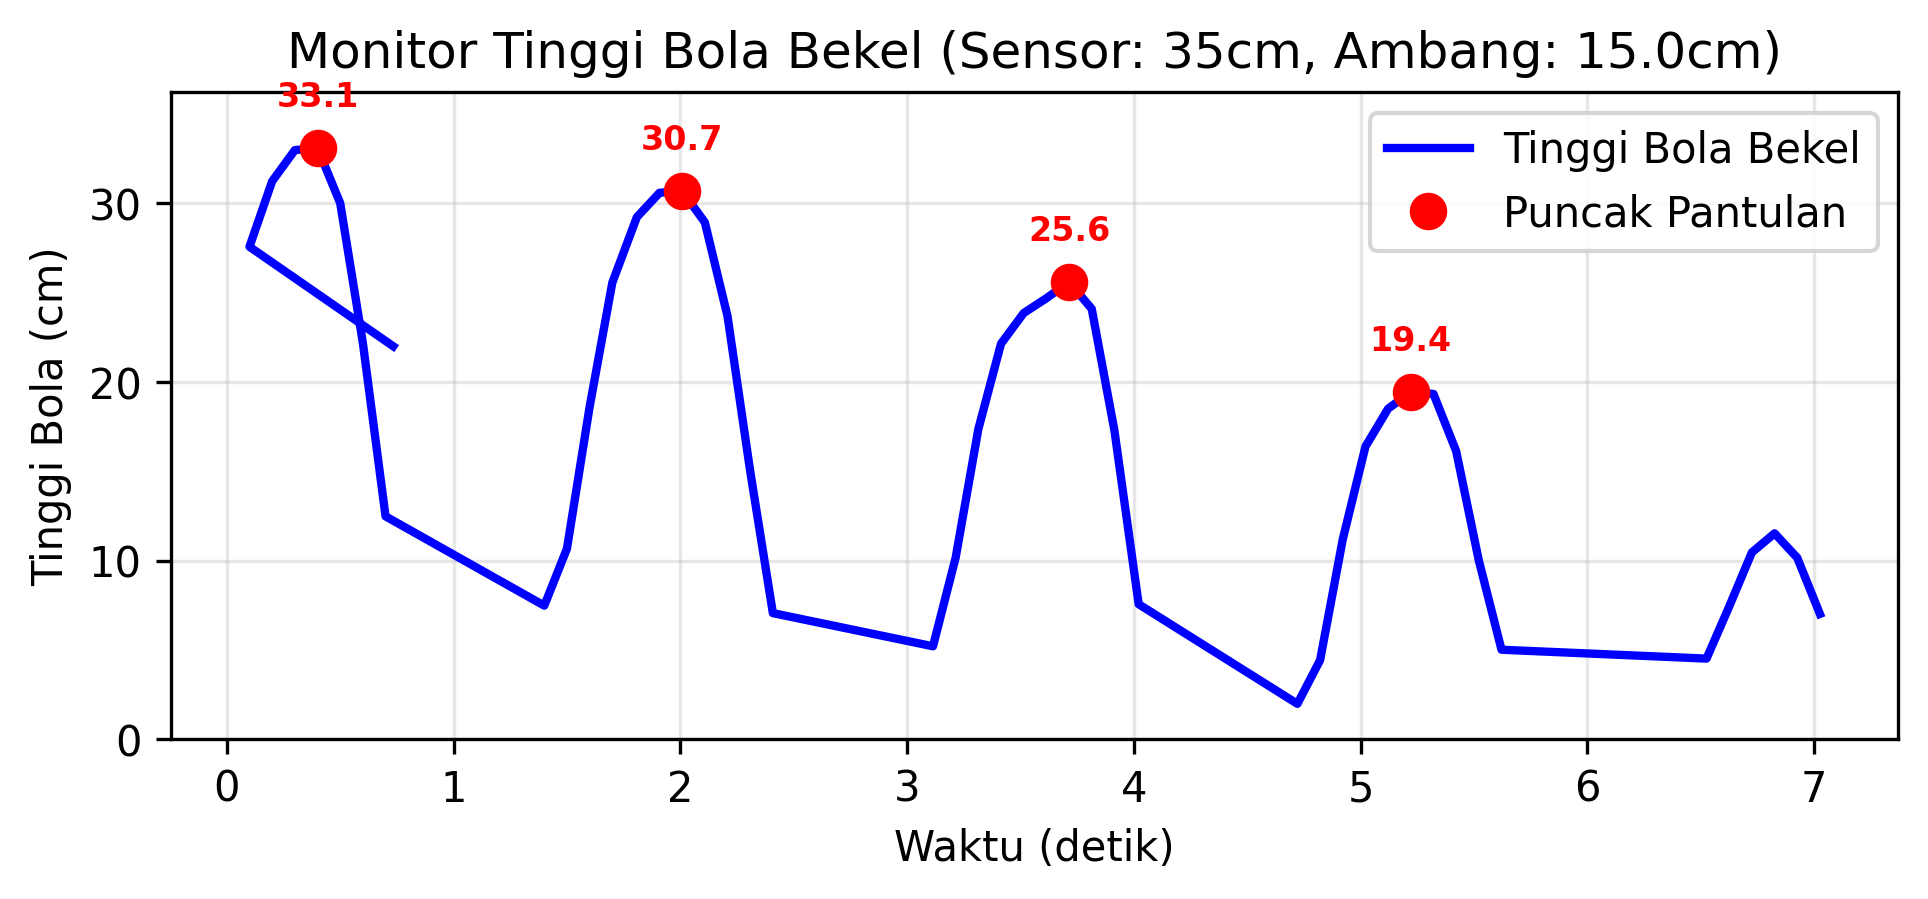
\includegraphics[width=0.5\textwidth]{chapters/DataPercobaan/Grafik_Bola_Bekel_1.png}
    \caption{Grafik Bola Bekel Percobaan 1}
\end{figure}
\begin{figure}[htbp]
    \centering
    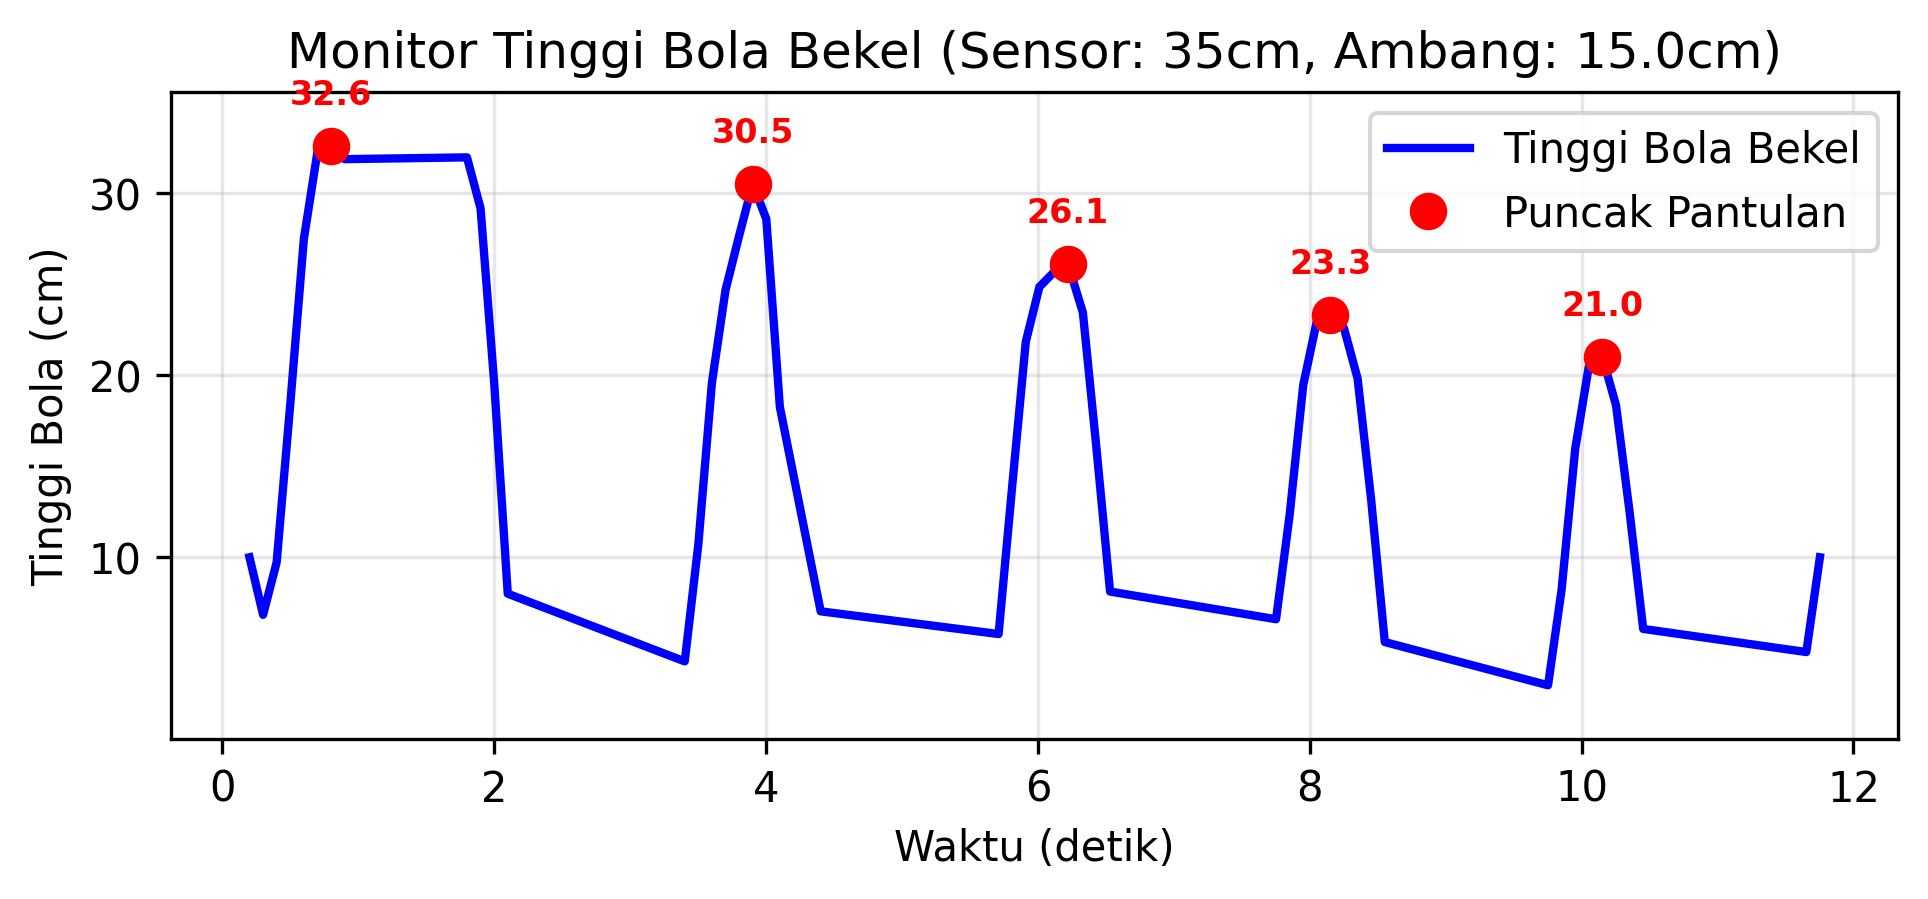
\includegraphics[width=0.5\textwidth]{chapters/DataPercobaan/Grafik_Bola_Bekel_2.png}
    \caption{Grafik Bola Bekel Percobaan 2}
\end{figure}
\begin{figure}[htbp]
    \centering
    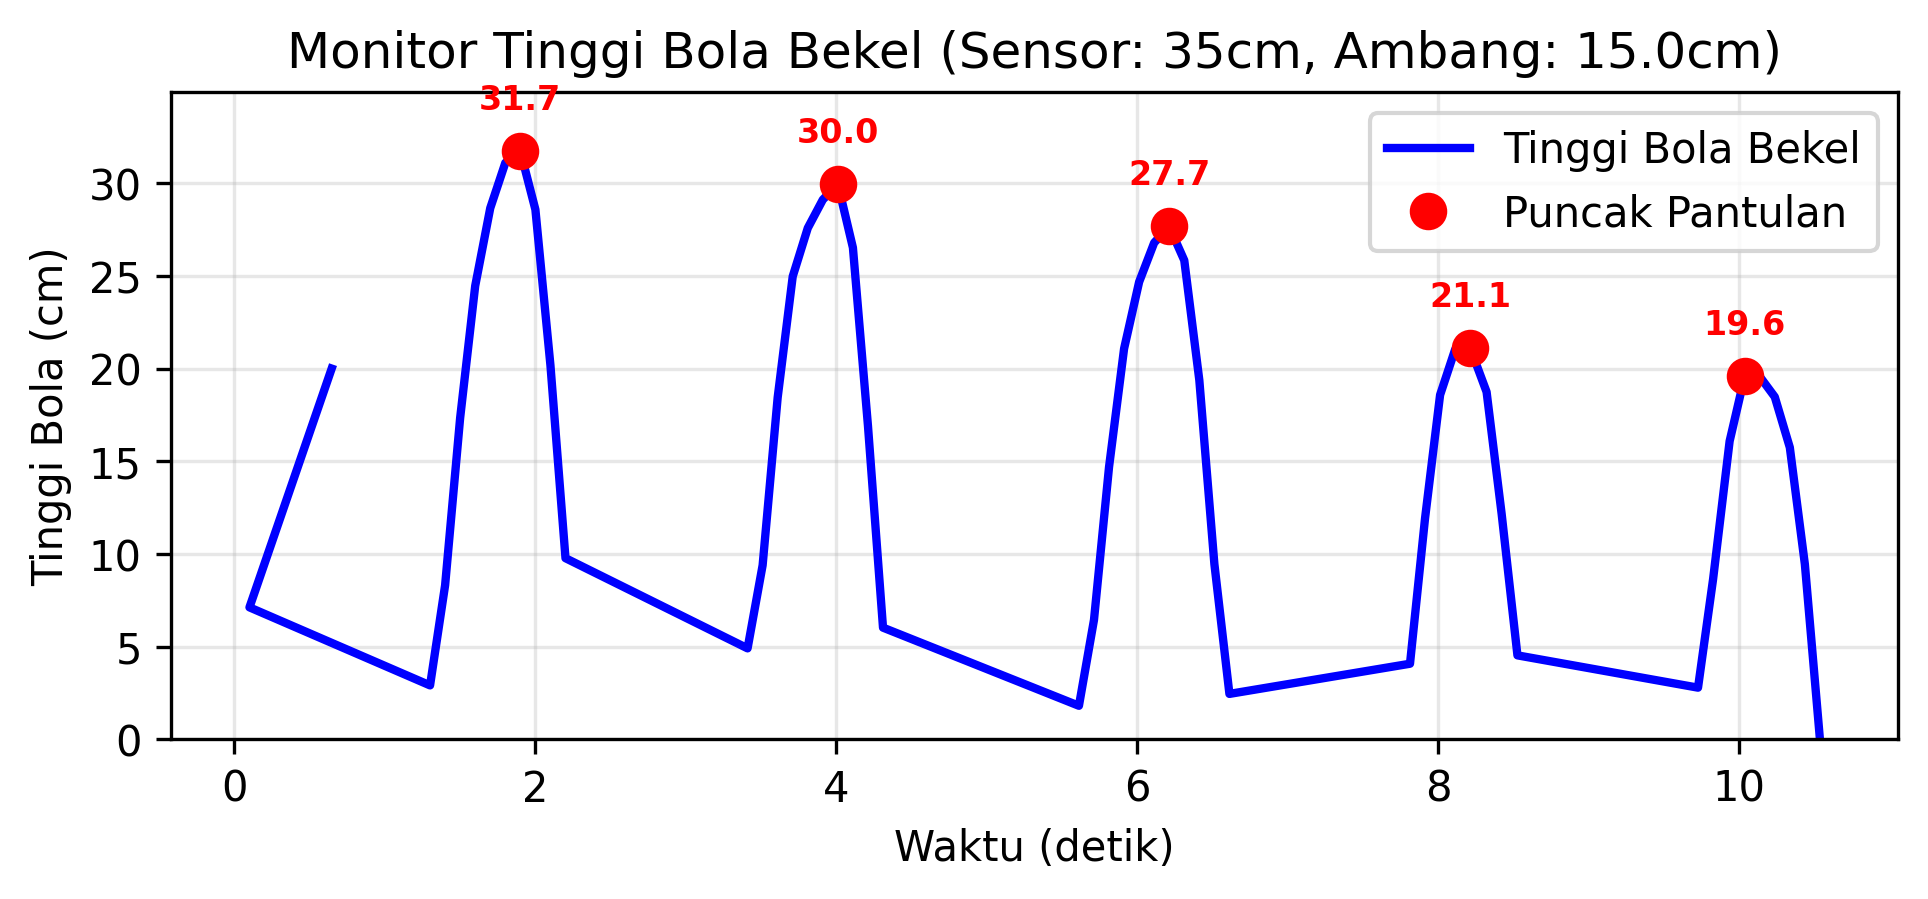
\includegraphics[width=0.5\textwidth]{chapters/DataPercobaan/Grafik_Bola_Bekel_3.png}
    \caption{Grafik Bola Bekel Percobaan 3}
\end{figure}
\begin{figure}[htbp]
    \centering
    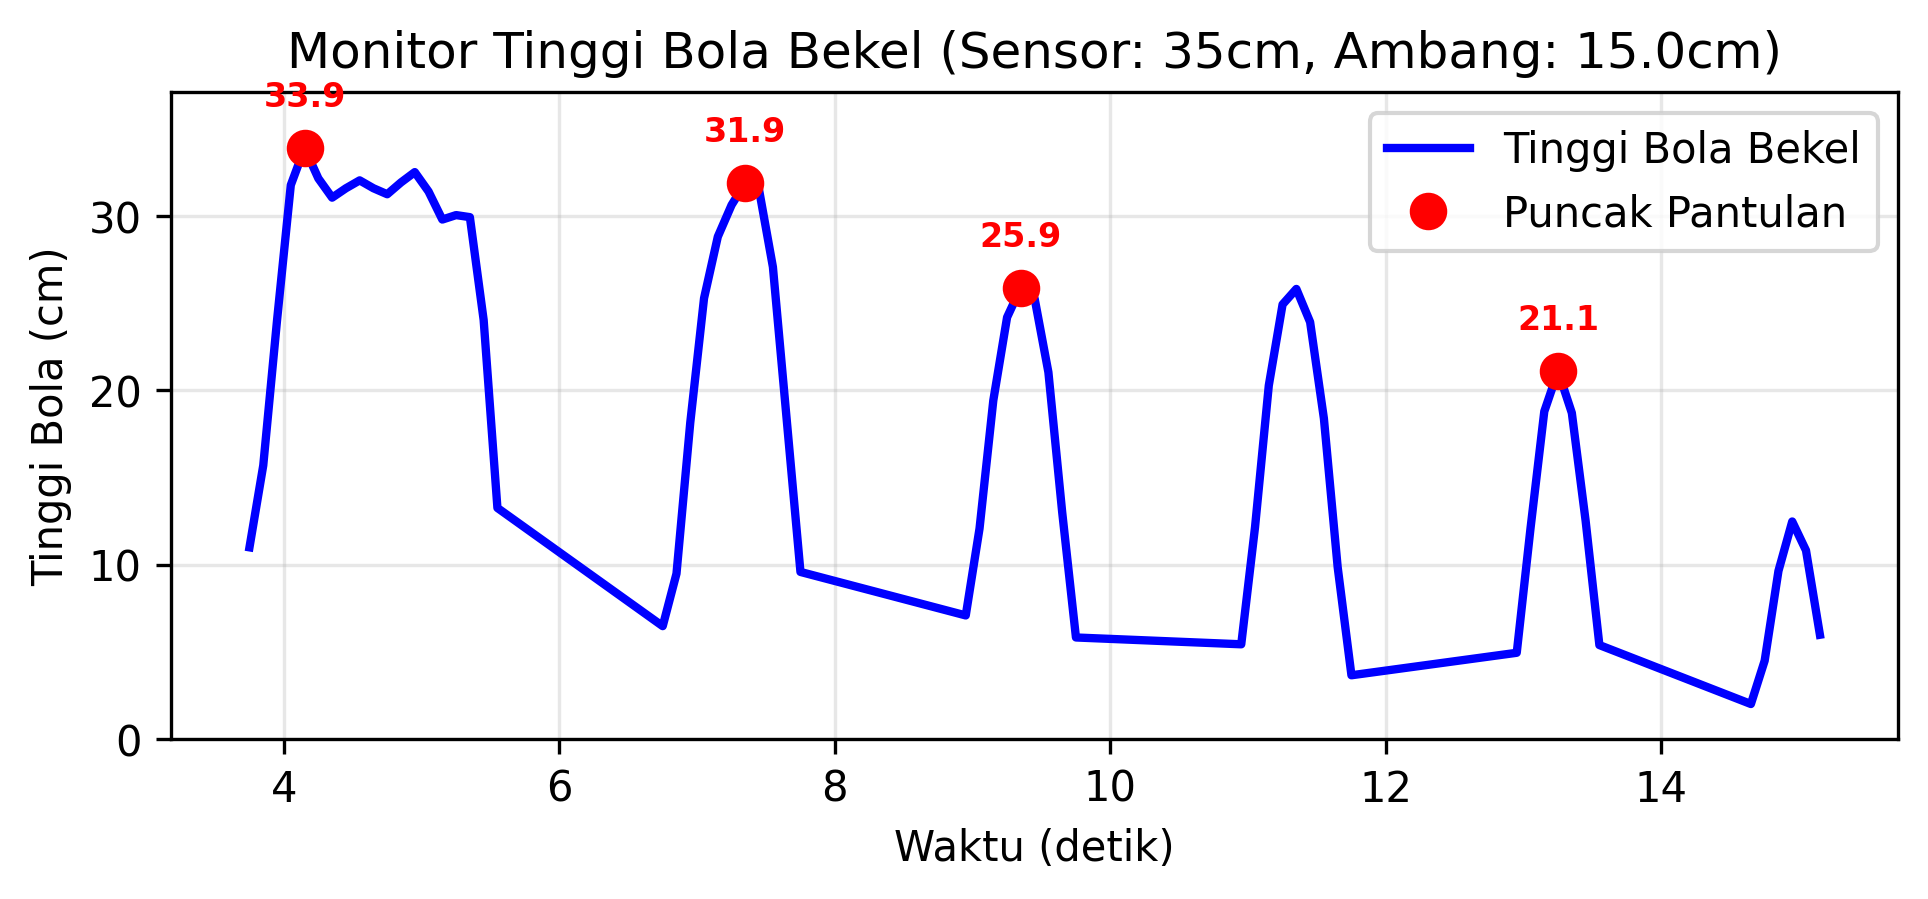
\includegraphics[width=0.5\textwidth]{chapters/DataPercobaan/Grafik_Bola_Bekel_4.png}
    \caption{Grafik Bola Bekel Percobaan 4}
\end{figure}
\begin{figure}[htbp]
    \centering
    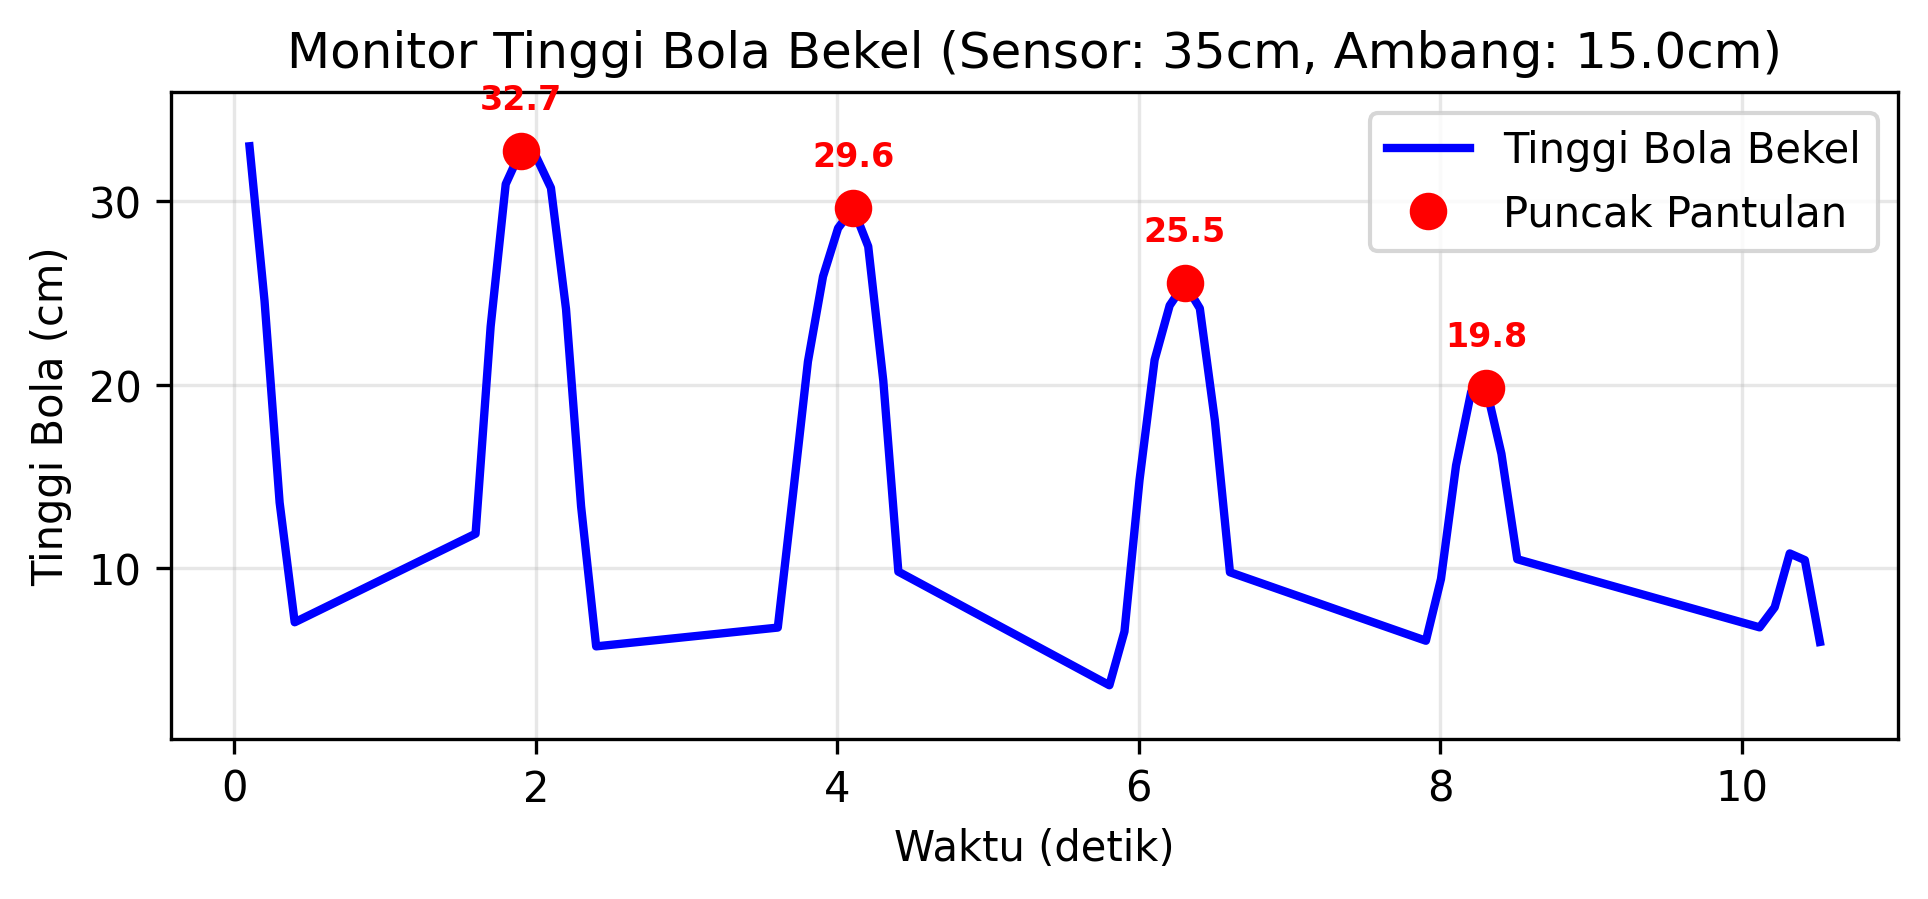
\includegraphics[width=0.5\textwidth]{chapters/DataPercobaan/Grafik_Bola_Bekel_5.png}
    \caption{Grafik Bola Bekel Percobaan 5}
\end{figure}
\begin{figure}[htbp]
    \centering
    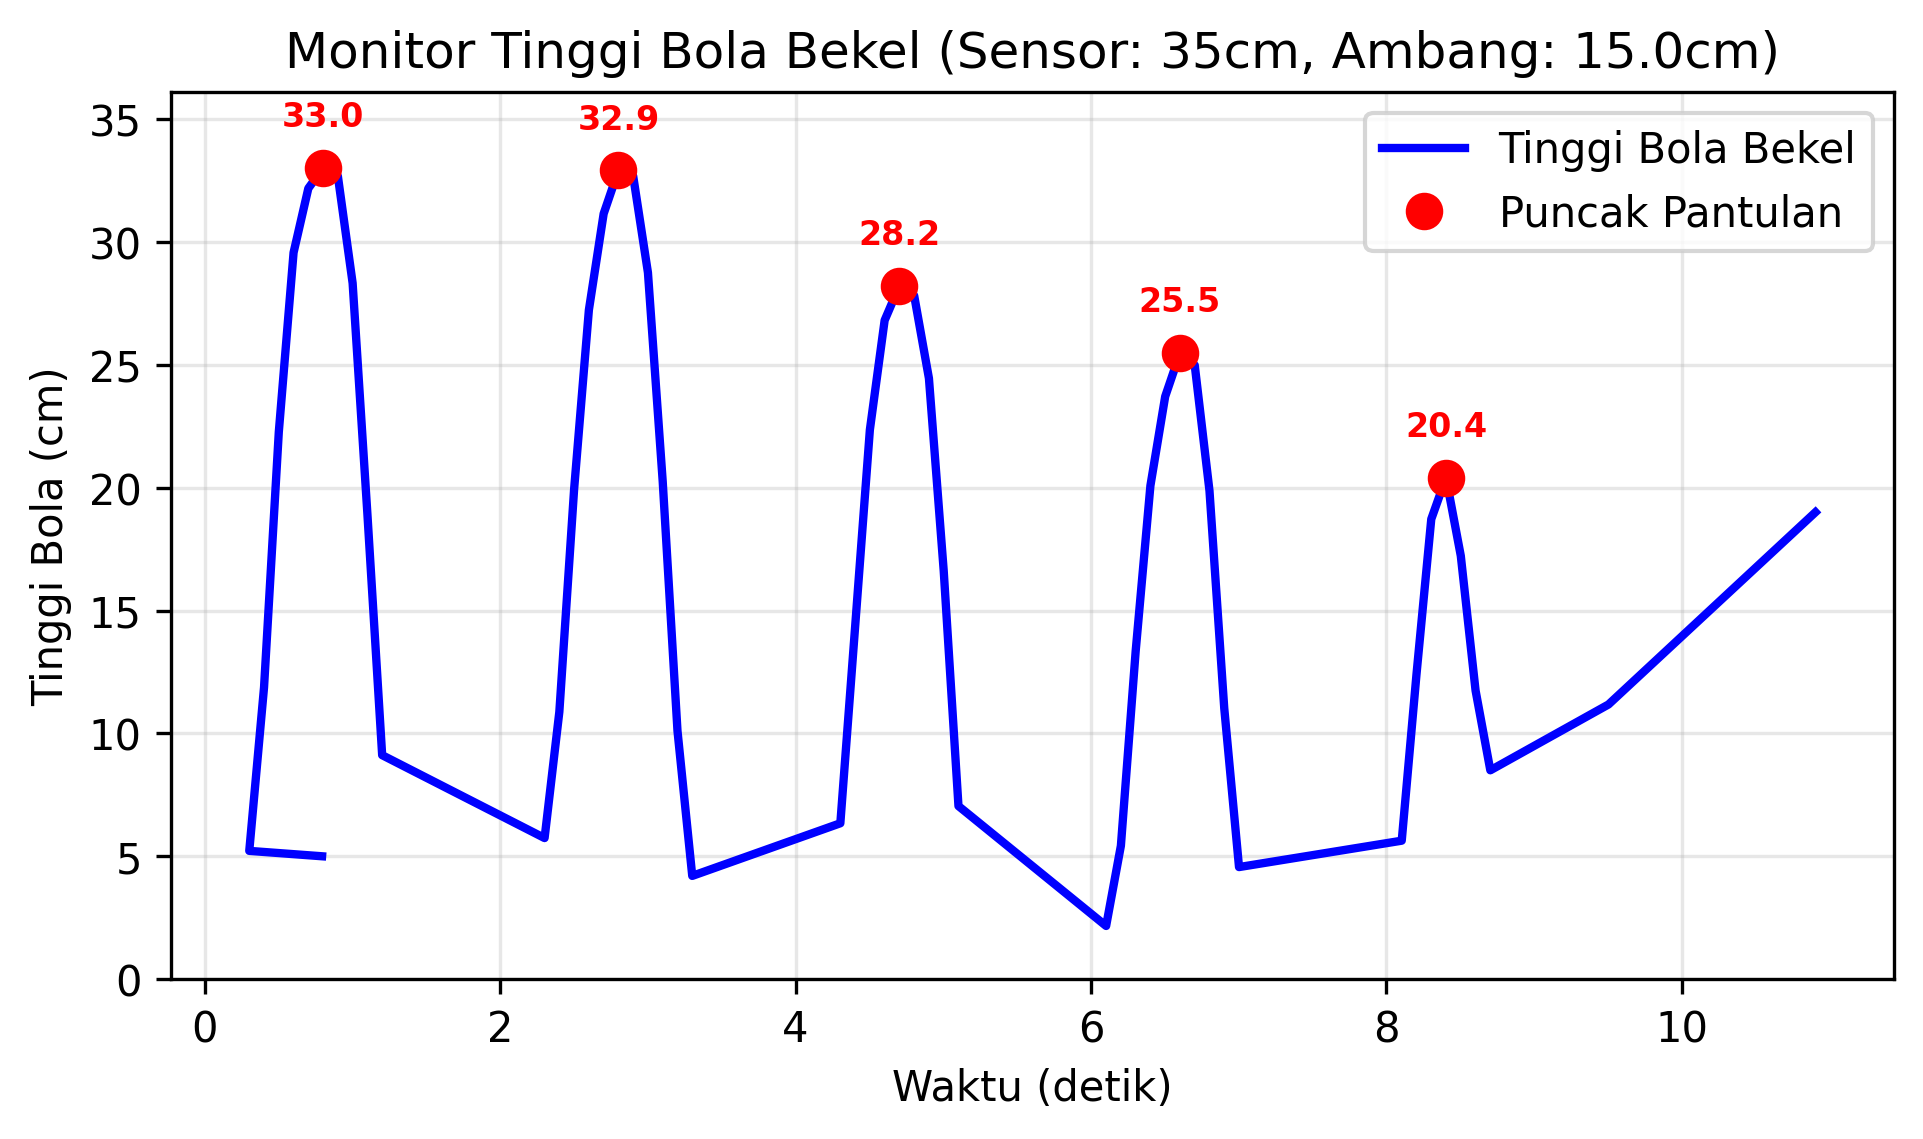
\includegraphics[width=0.5\textwidth]{chapters/DataPercobaan/Grafik_Bola_Bekel_6.png}
    \caption{Grafik Bola Bekel Percobaan 6}
\end{figure}
\begin{figure}[htbp]
    \centering
    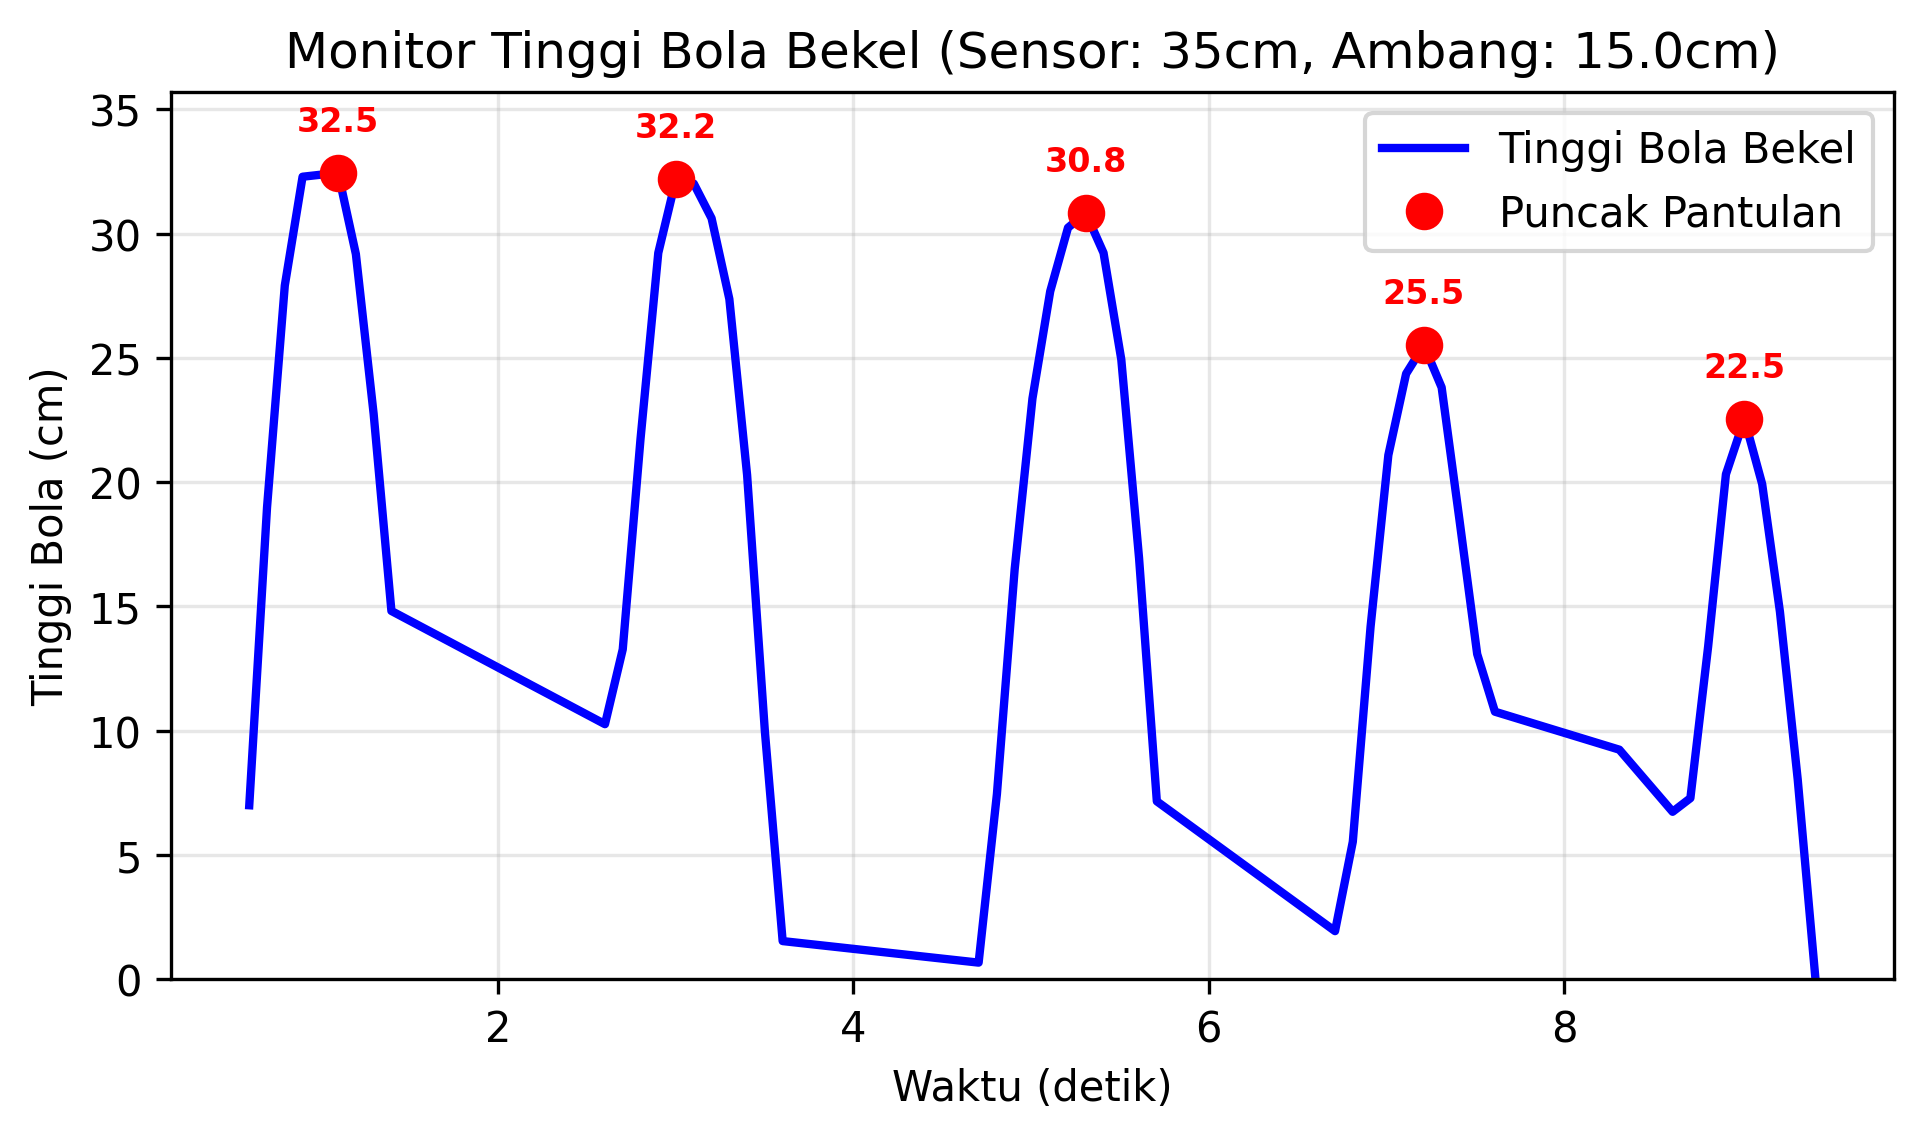
\includegraphics[width=0.5\textwidth]{chapters/DataPercobaan/Grafik_Bola_Bekel_7.png}
    \caption{Grafik Bola Bekel Percobaan 7}
\end{figure}
\begin{figure}[htbp]
    \centering
    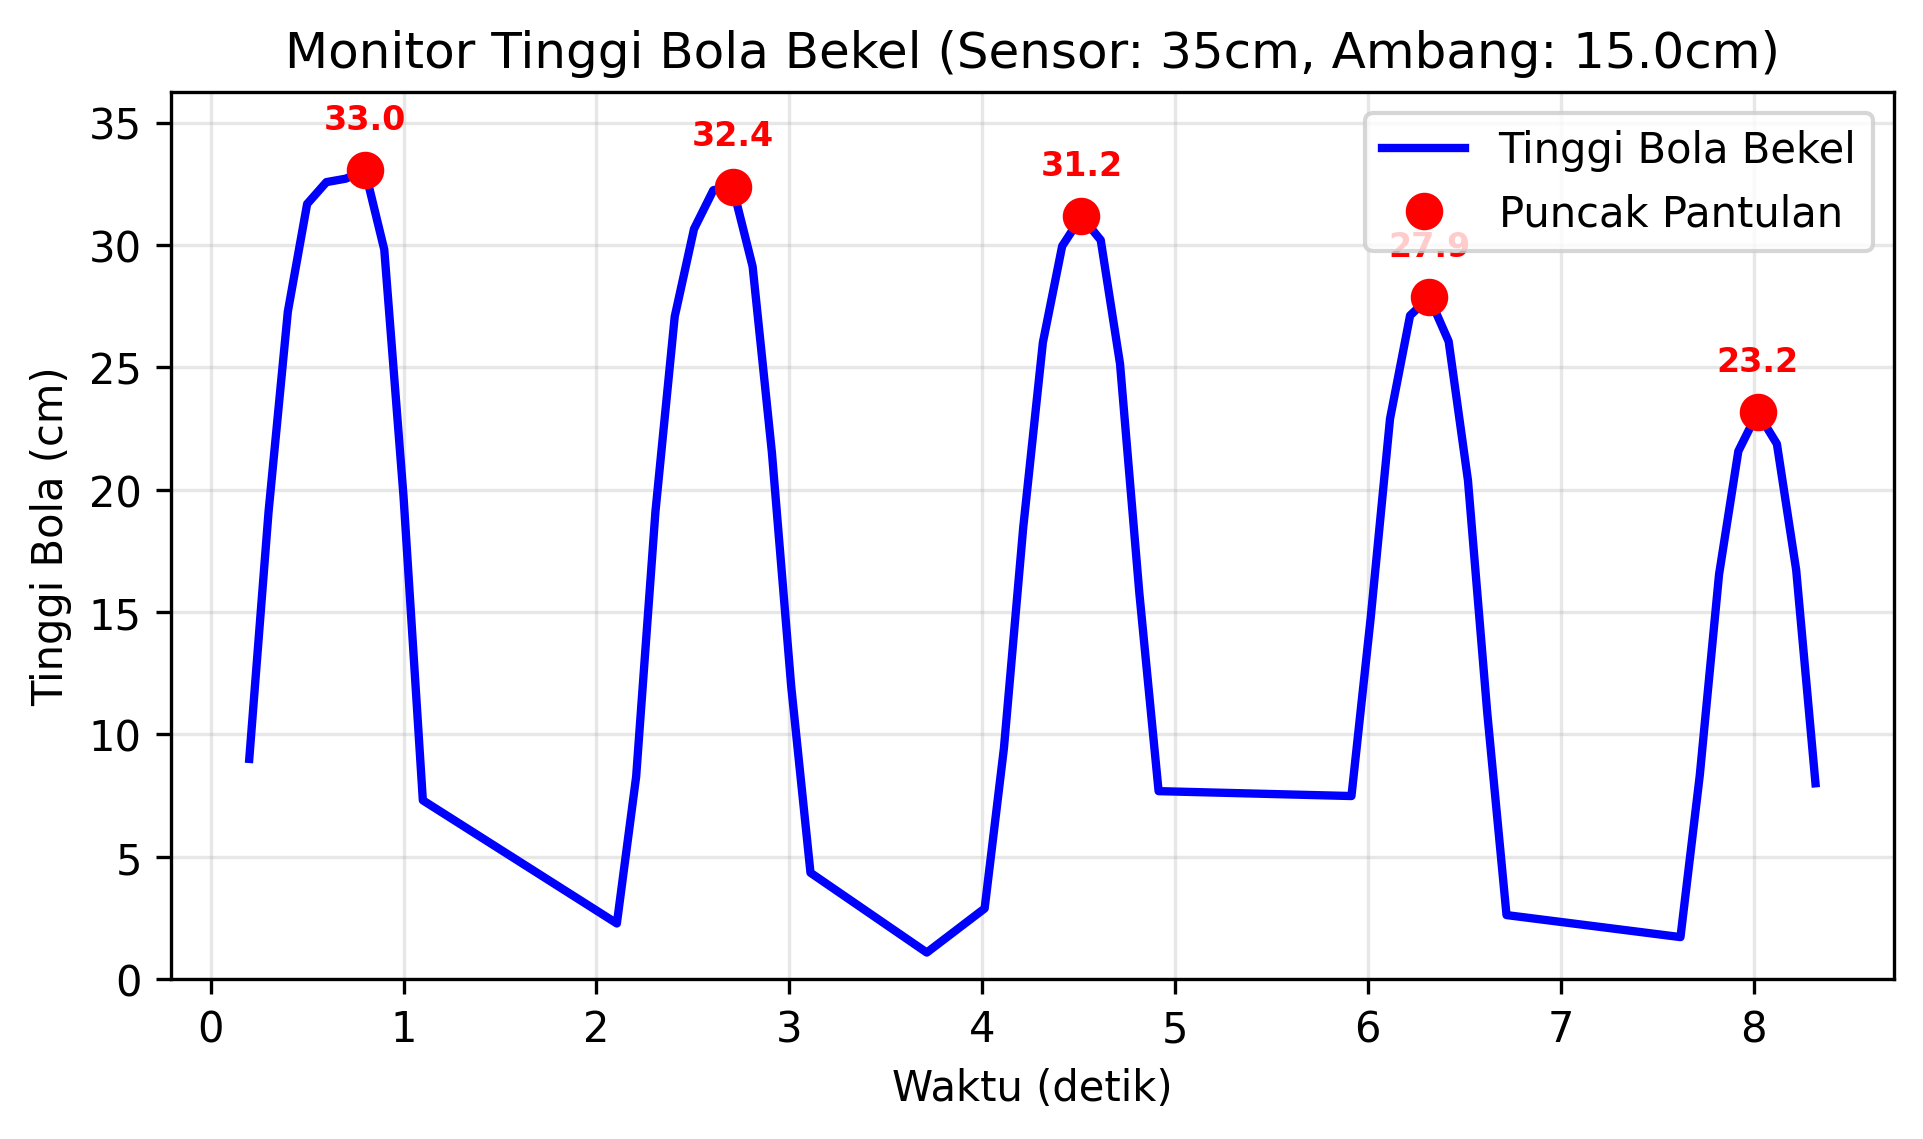
\includegraphics[width=0.5\textwidth]{chapters/DataPercobaan/Grafik_Bola_Bekel_8.png}
    \caption{Grafik Bola Bekel Percobaan 8}
\end{figure}
\begin{figure}[htbp]
    \centering
    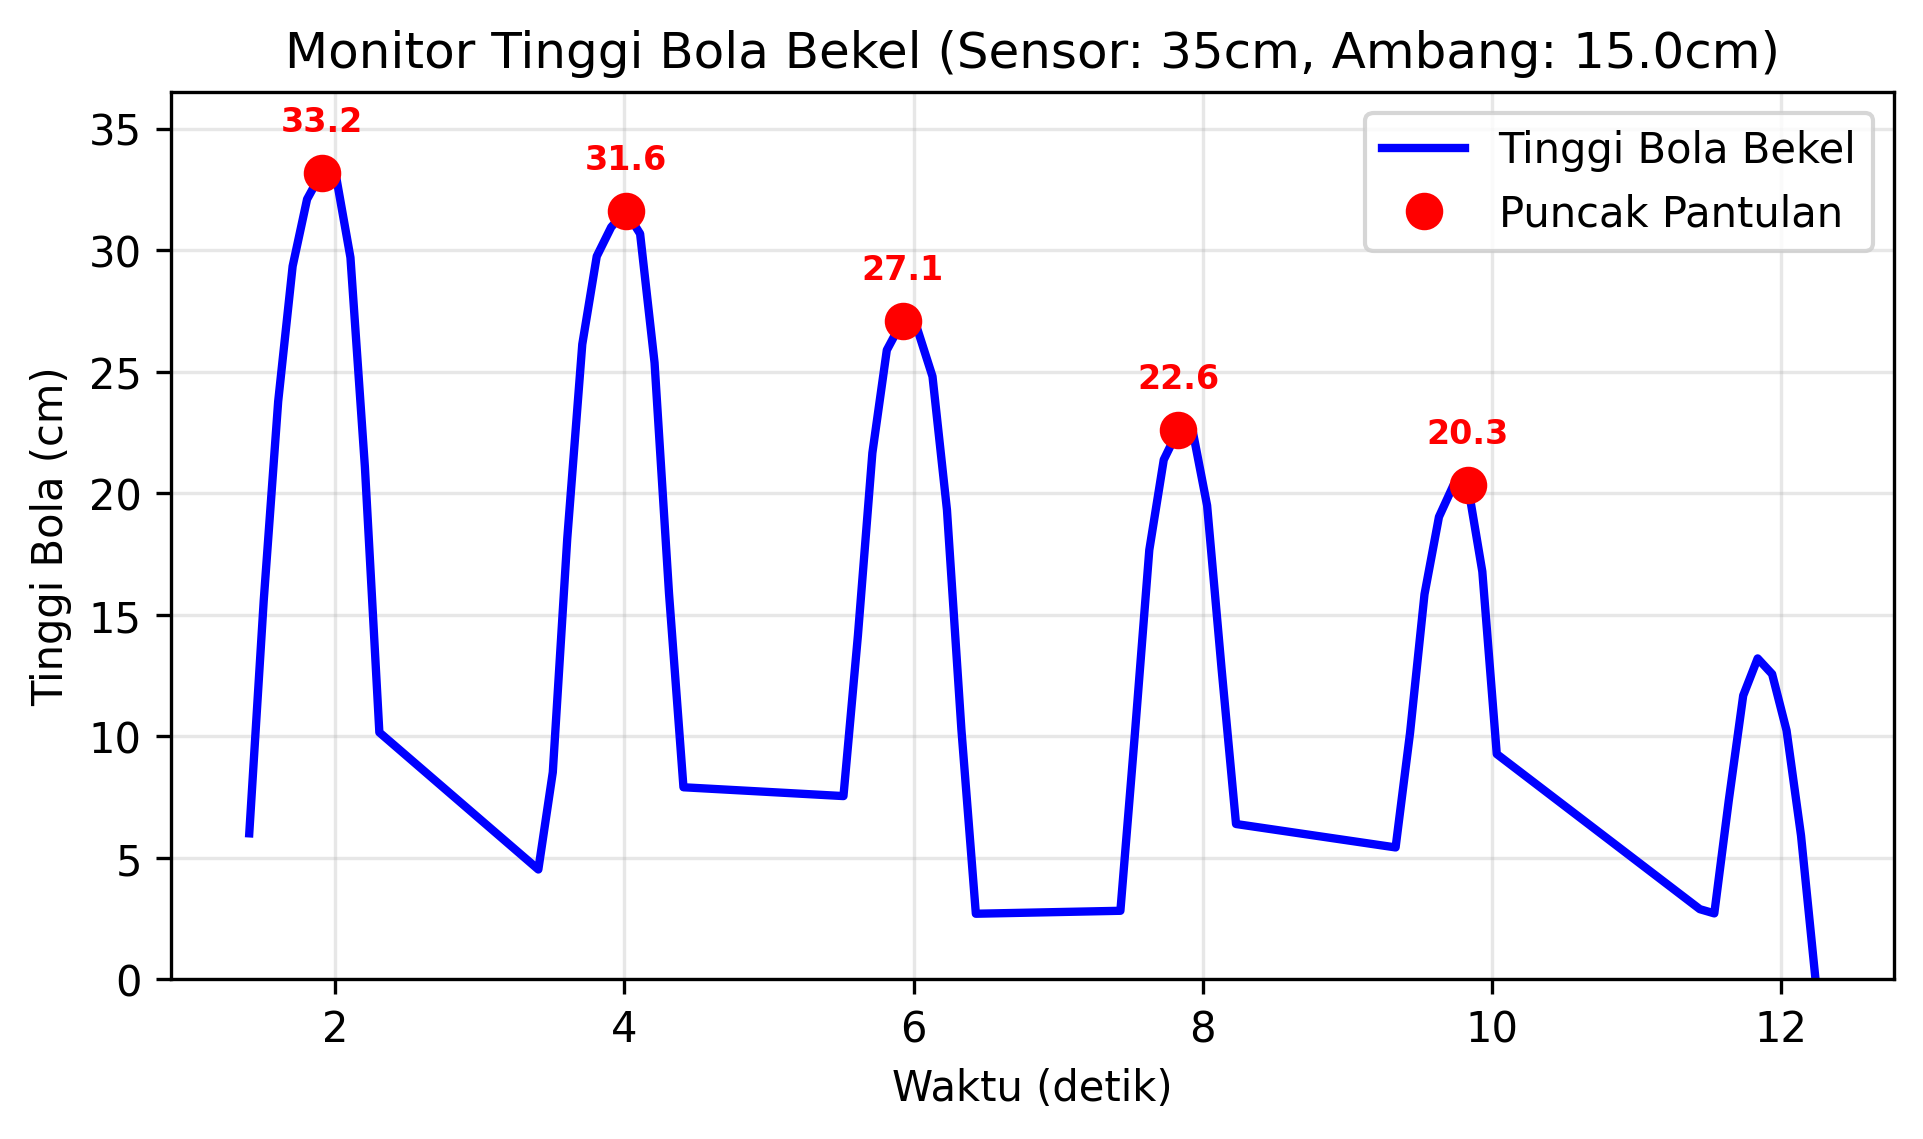
\includegraphics[width=0.5\textwidth]{chapters/DataPercobaan/Grafik_Bola_Bekel_9.png}
    \caption{Grafik Bola Bekel Percobaan 9}
\end{figure}
\begin{figure}[htbp]
    \centering
    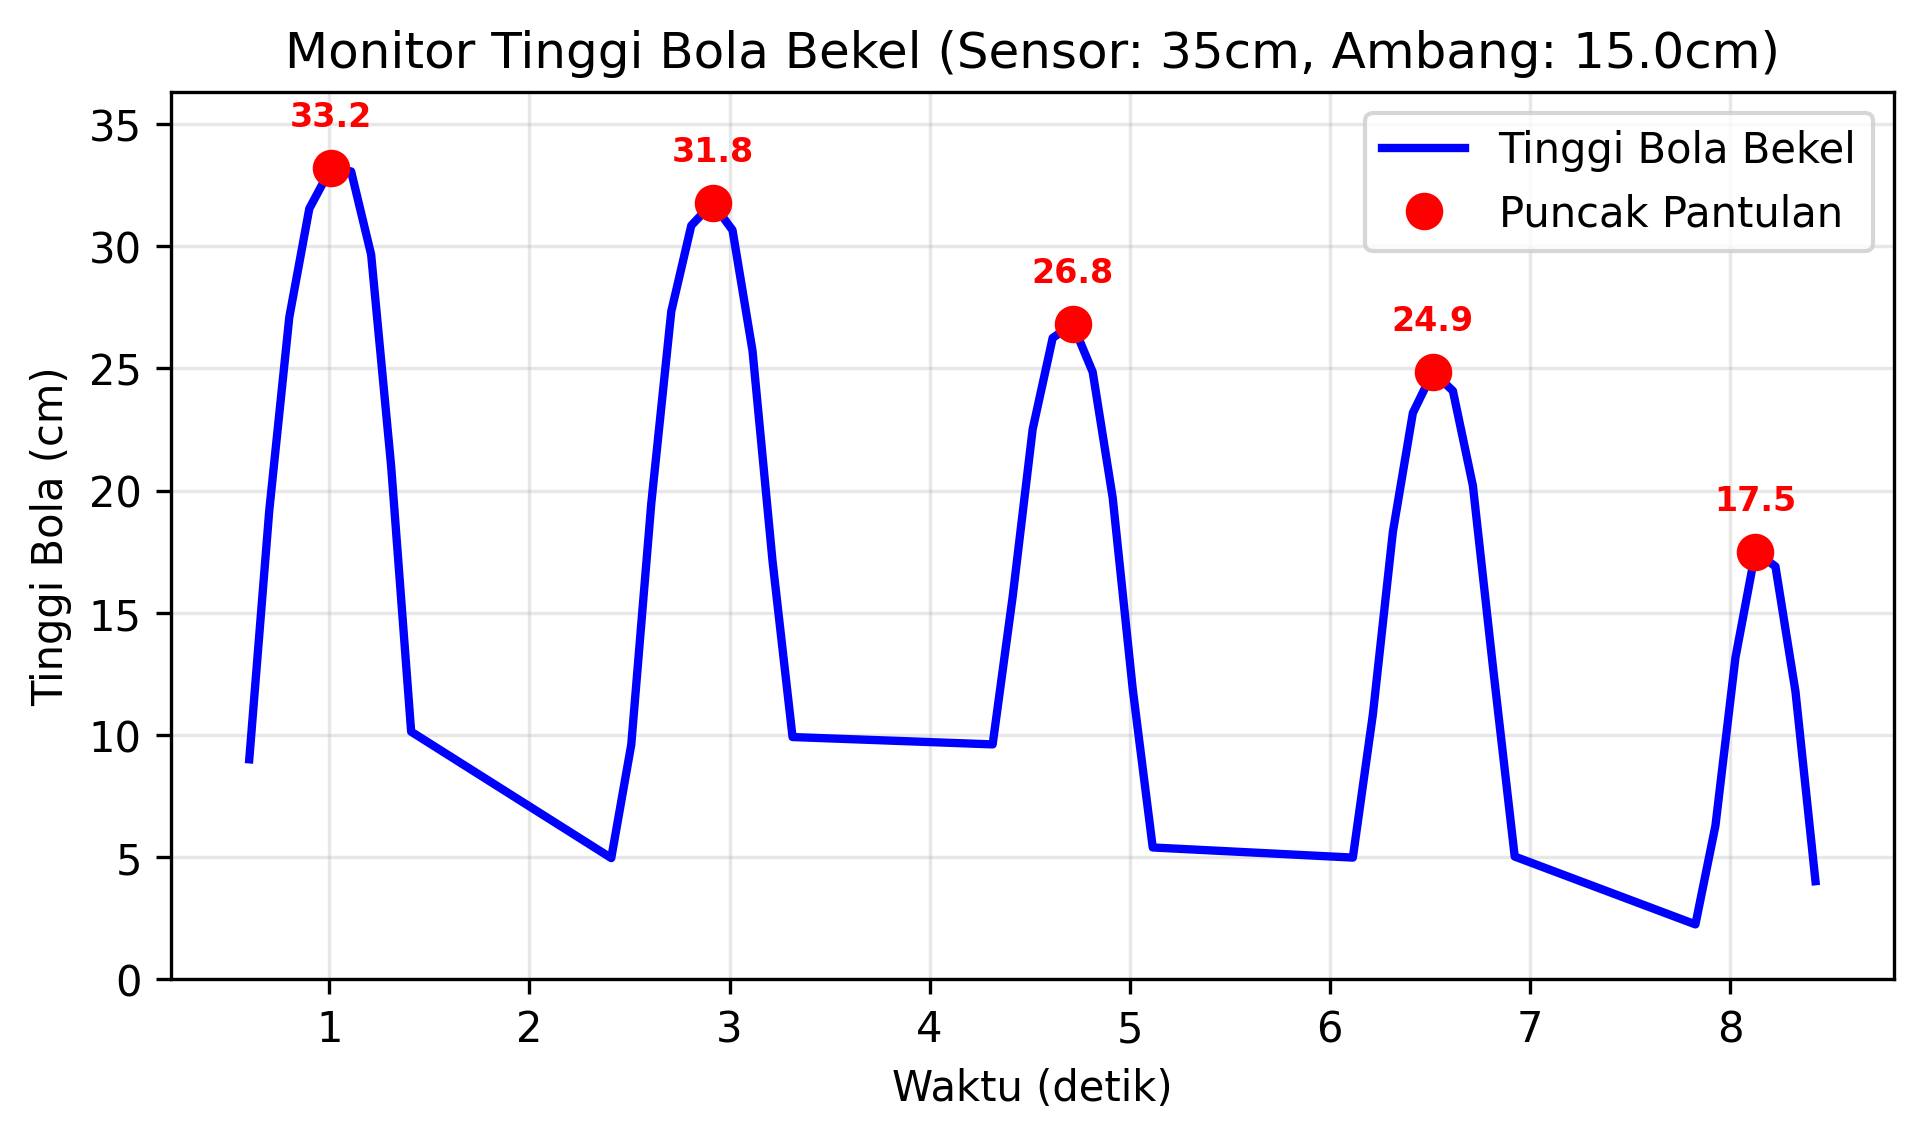
\includegraphics[width=0.5\textwidth]{chapters/DataPercobaan/Grafik_Bola_Bekel_10.png}
    \caption{Grafik Bola Bekel Percobaan 10}
\end{figure}
\begin{figure}[htbp]
    \centering
    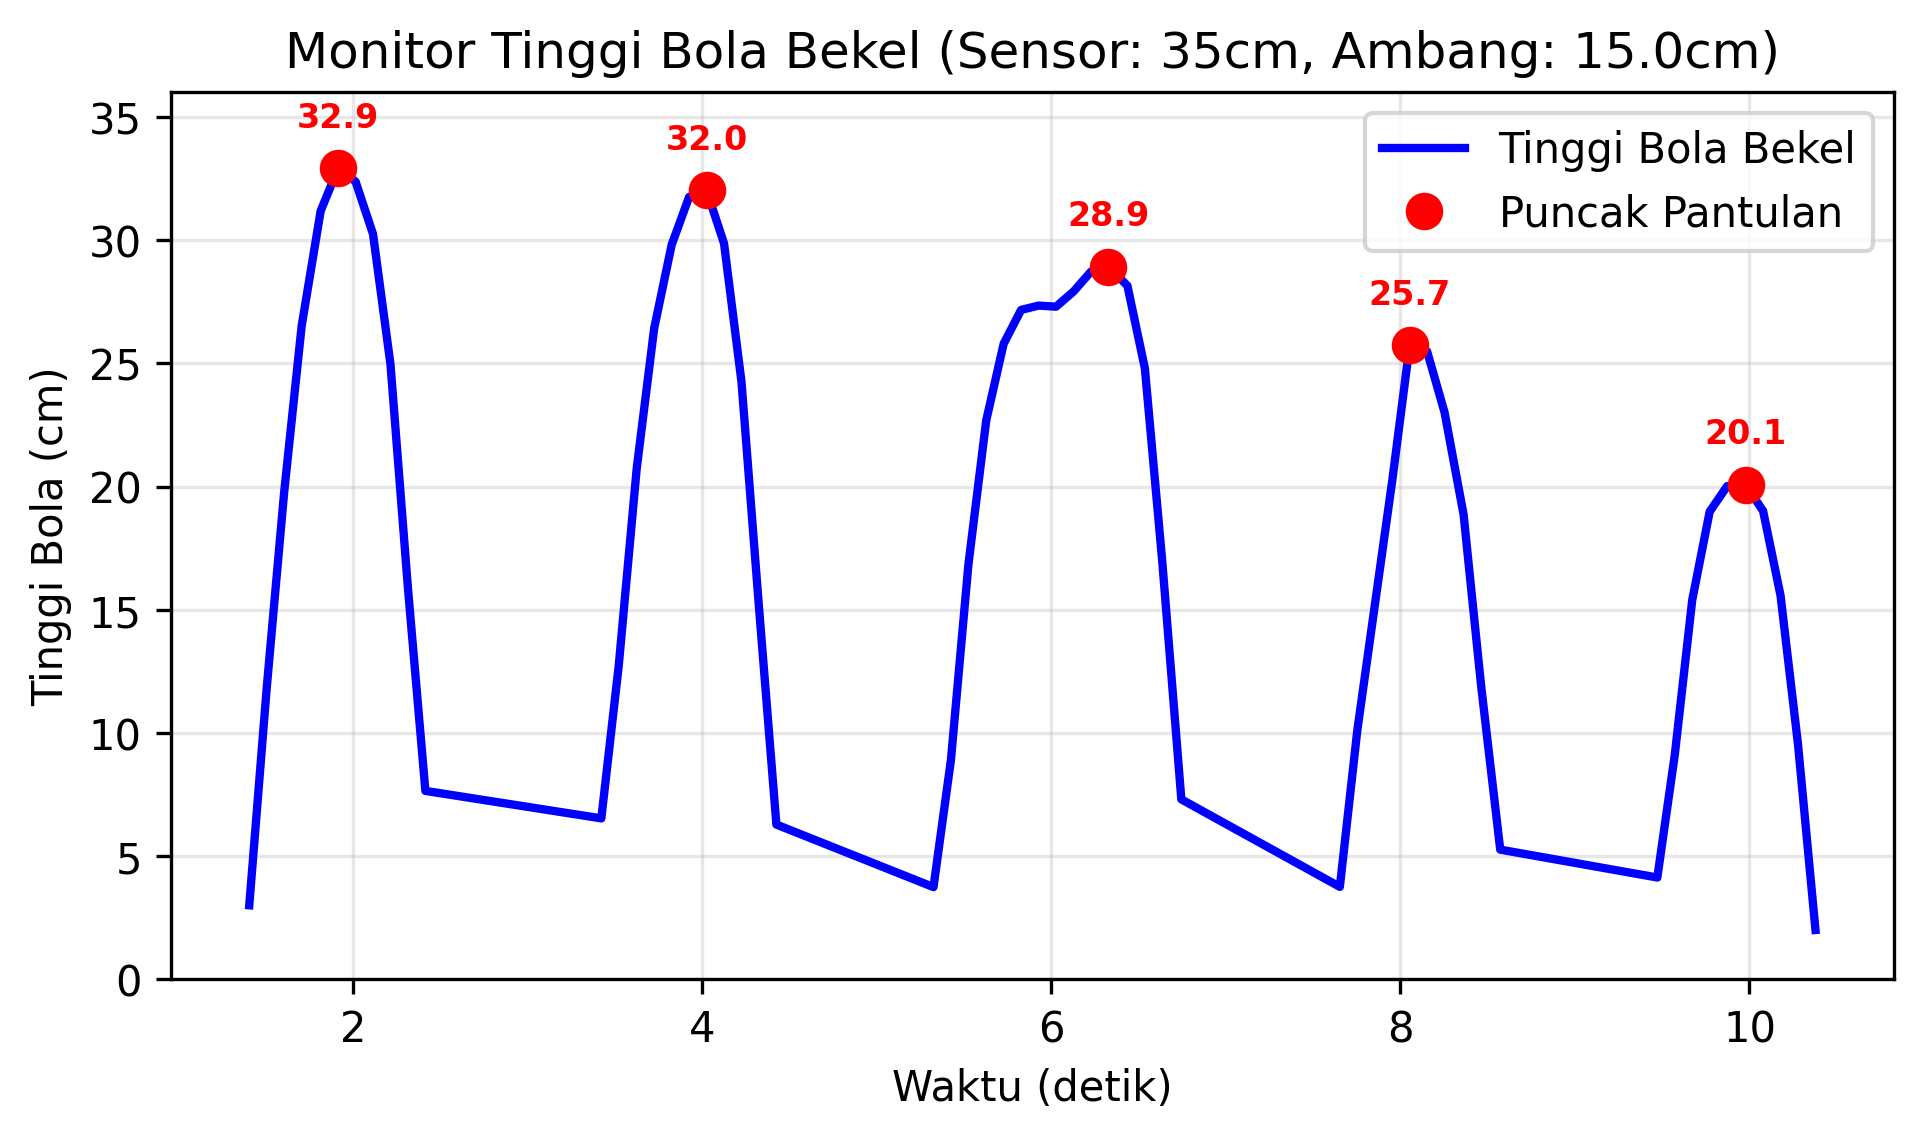
\includegraphics[width=0.5\textwidth]{chapters/DataPercobaan/Grafik_Bola_Bekel_11.png}
    \caption{Grafik Bola Bekel Percobaan 11}
\end{figure}
\begin{figure}[htbp]
    \centering
    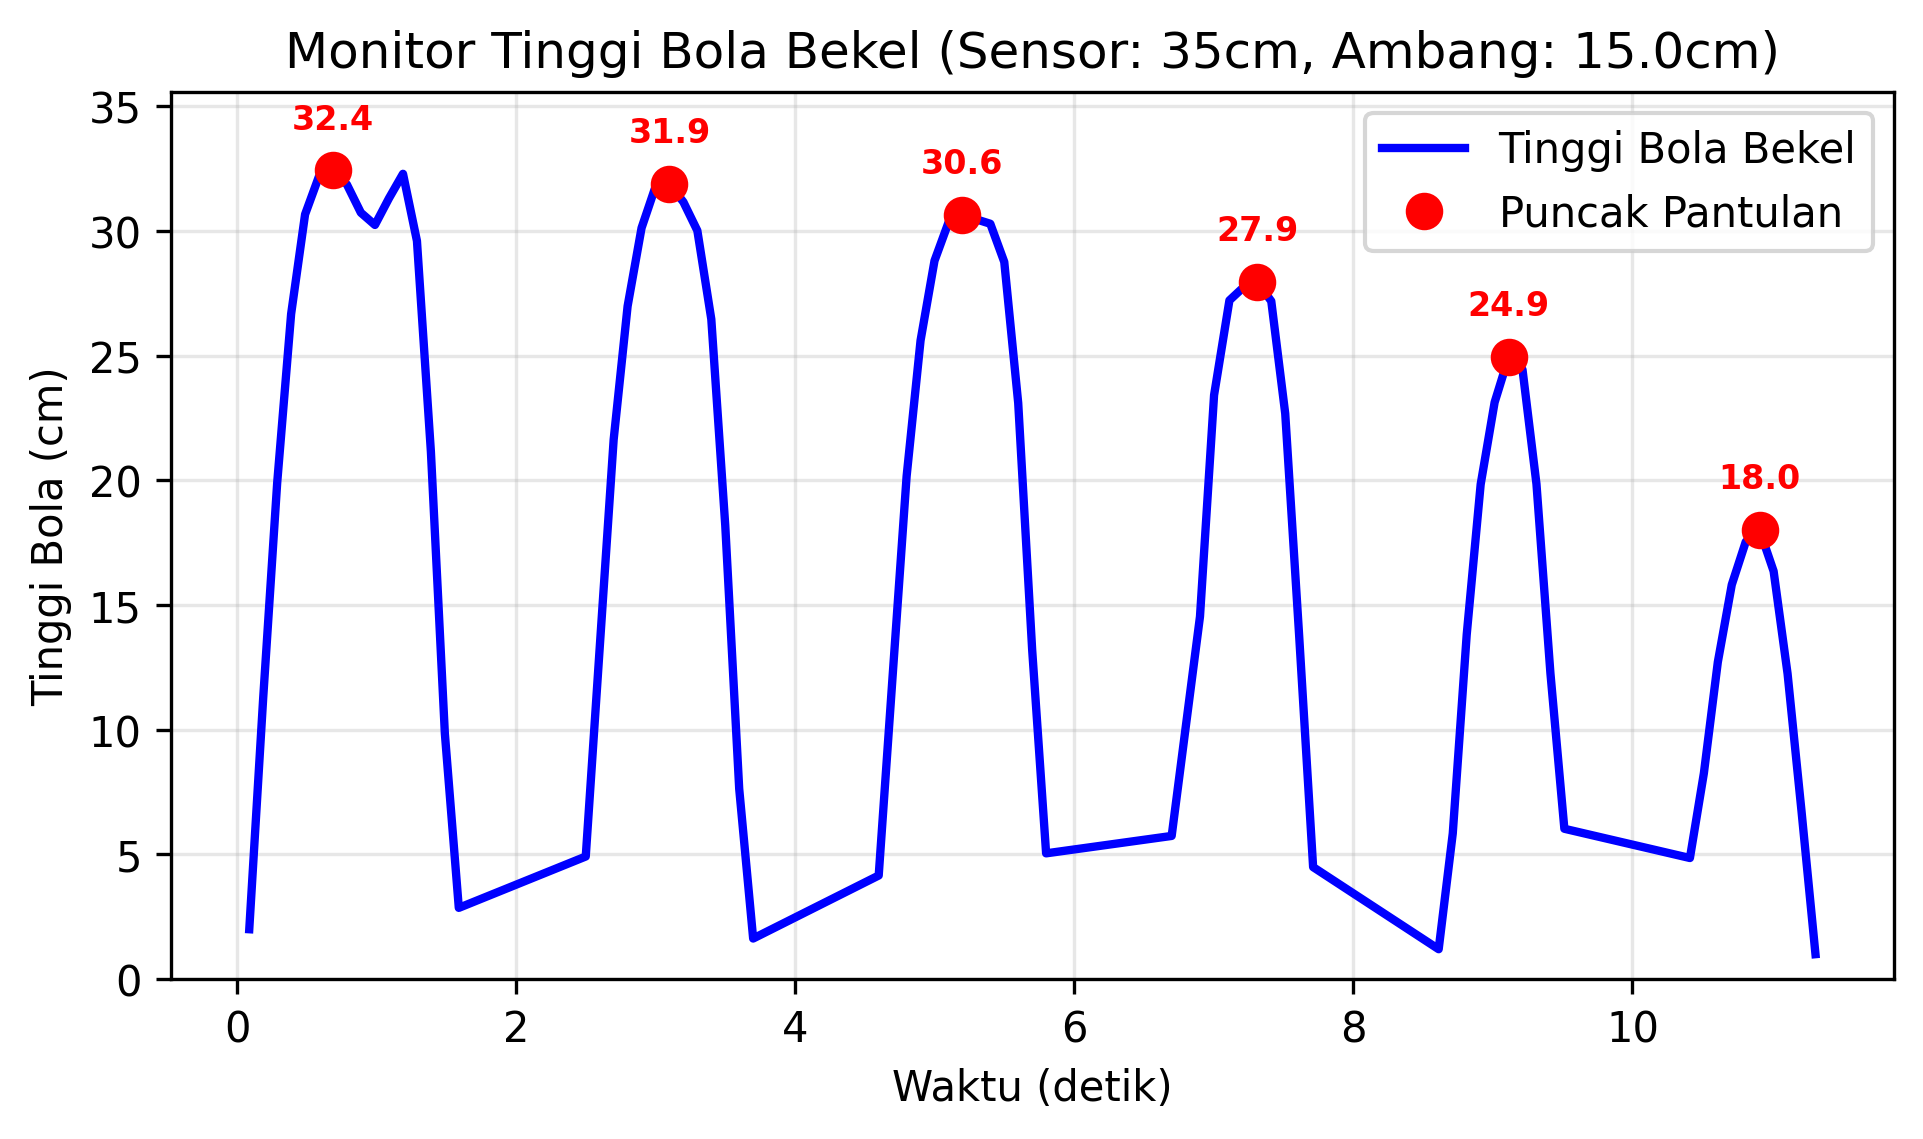
\includegraphics[width=0.5\textwidth]{chapters/DataPercobaan/Grafik_Bola_Bekel_12.png}
    \caption{Grafik Bola Bekel Percobaan 12}
\end{figure}
\begin{figure}[htbp]
    \centering
    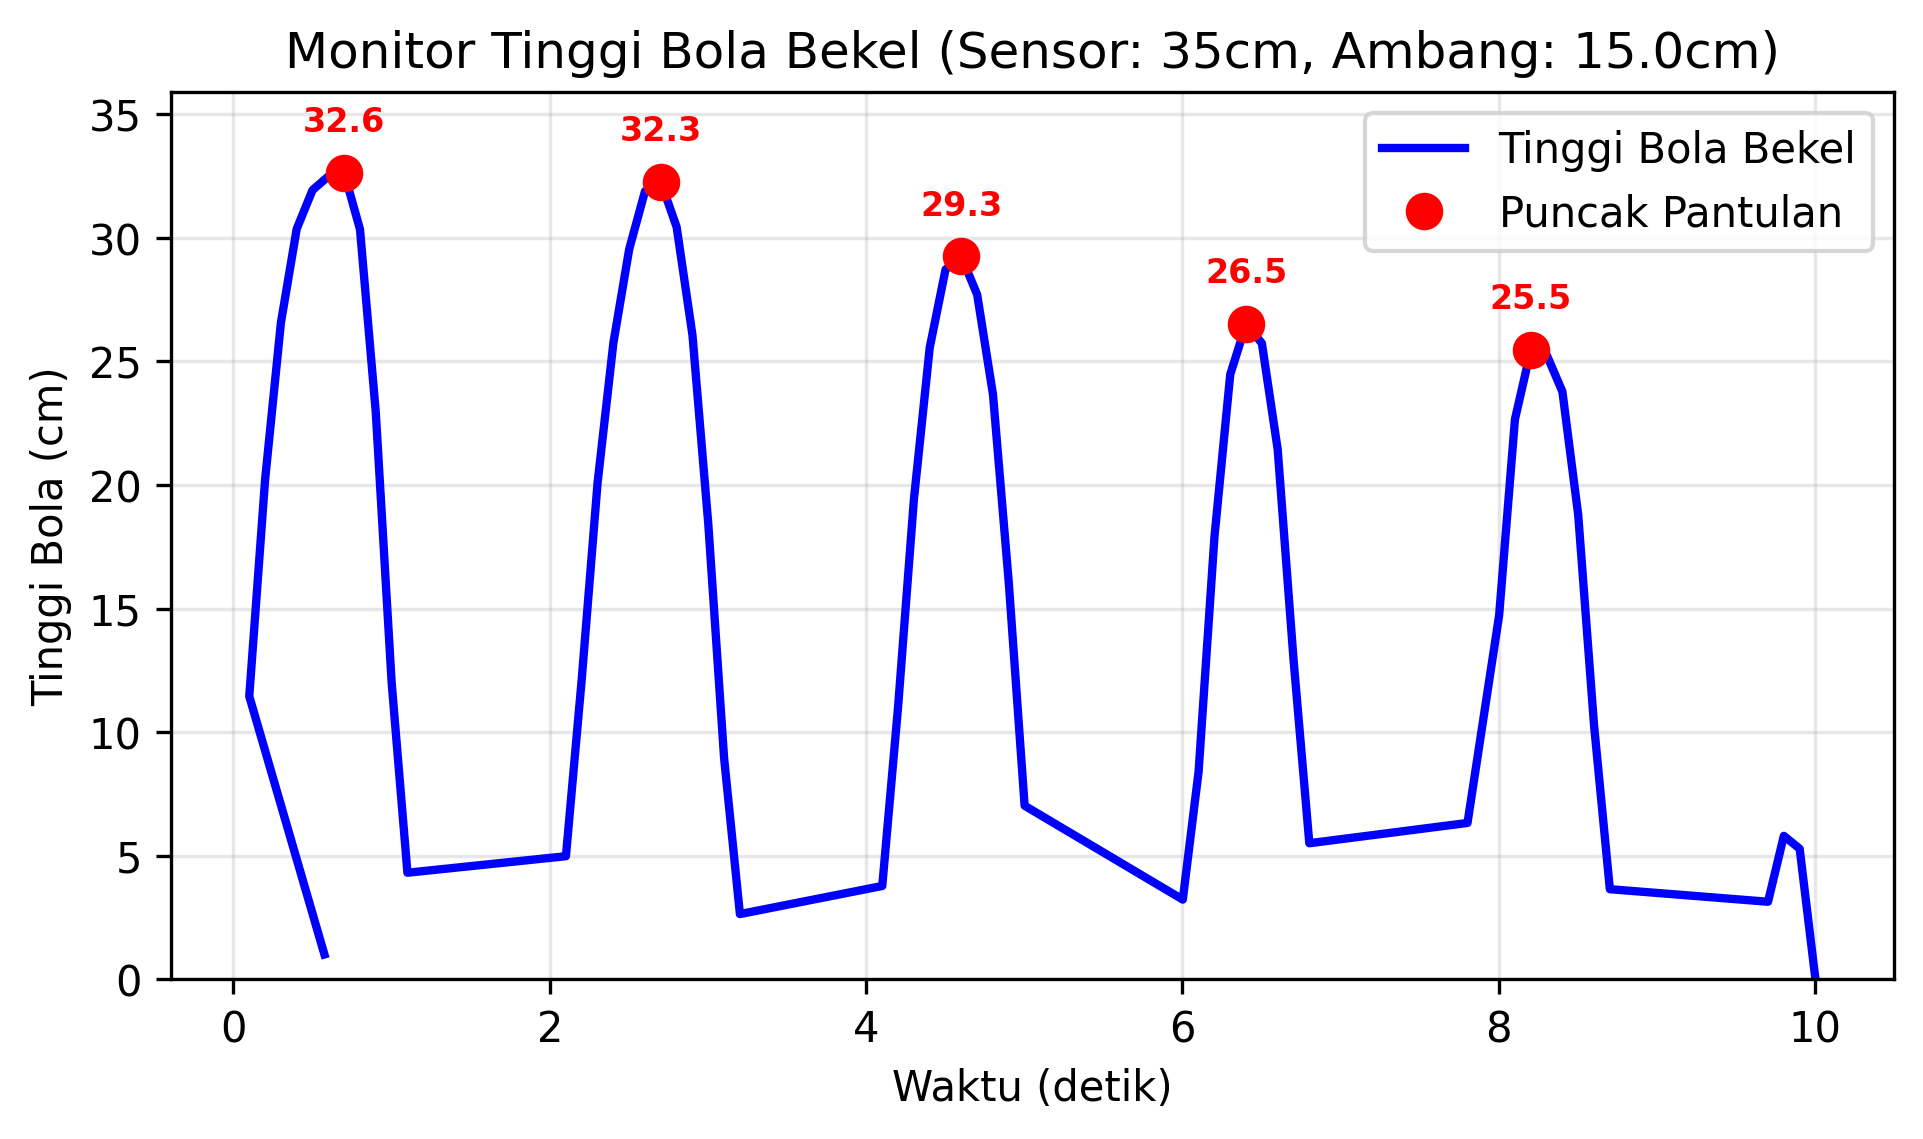
\includegraphics[width=0.5\textwidth]{chapters/DataPercobaan/Grafik_Bola_Bekel_13.png}
    \caption{Grafik Bola Bekel Percobaan 13}
\end{figure}
\begin{figure}[htbp]
    \centering
    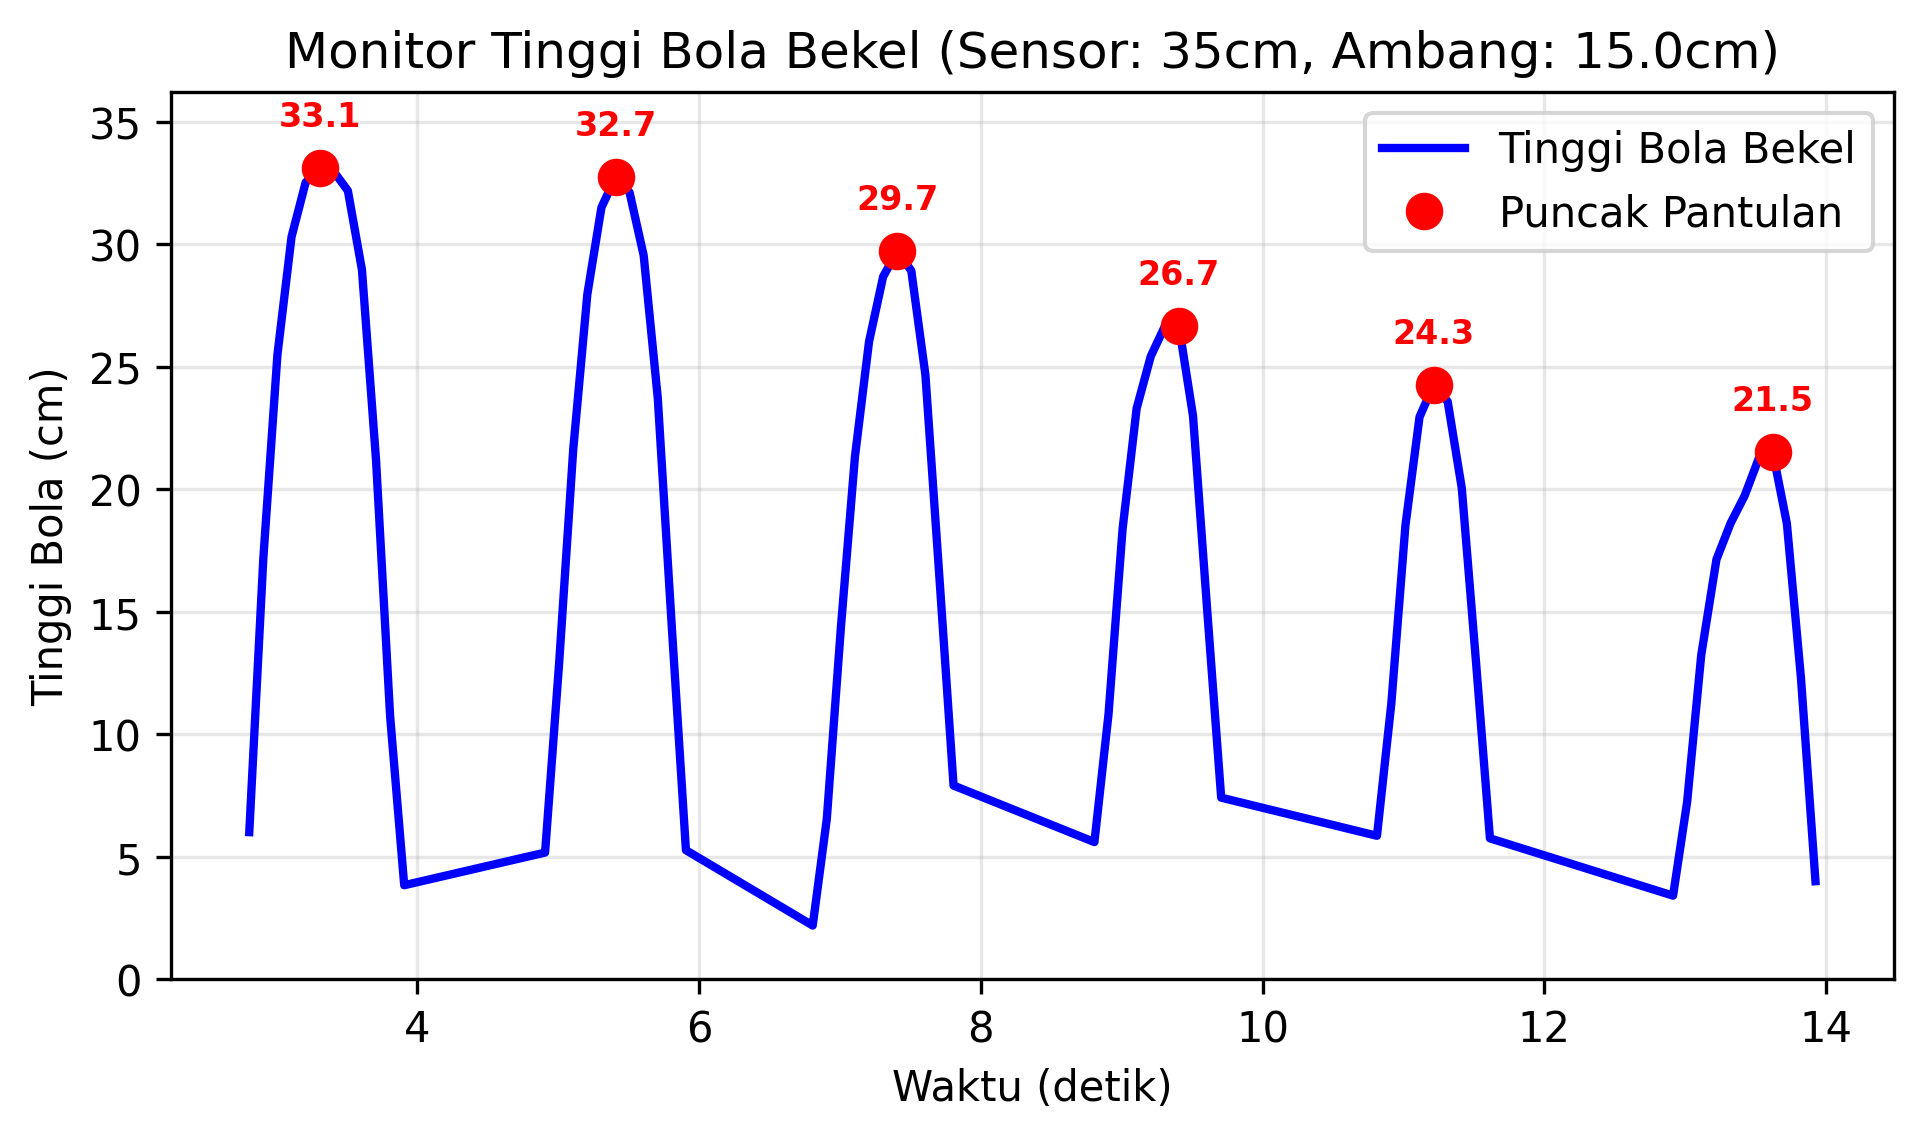
\includegraphics[width=0.5\textwidth]{chapters/DataPercobaan/Grafik_Bola_Bekel_14.png}
    \caption{Grafik Bola Bekel Percobaan 14}
\end{figure}
\begin{figure}[htbp]
    \centering
    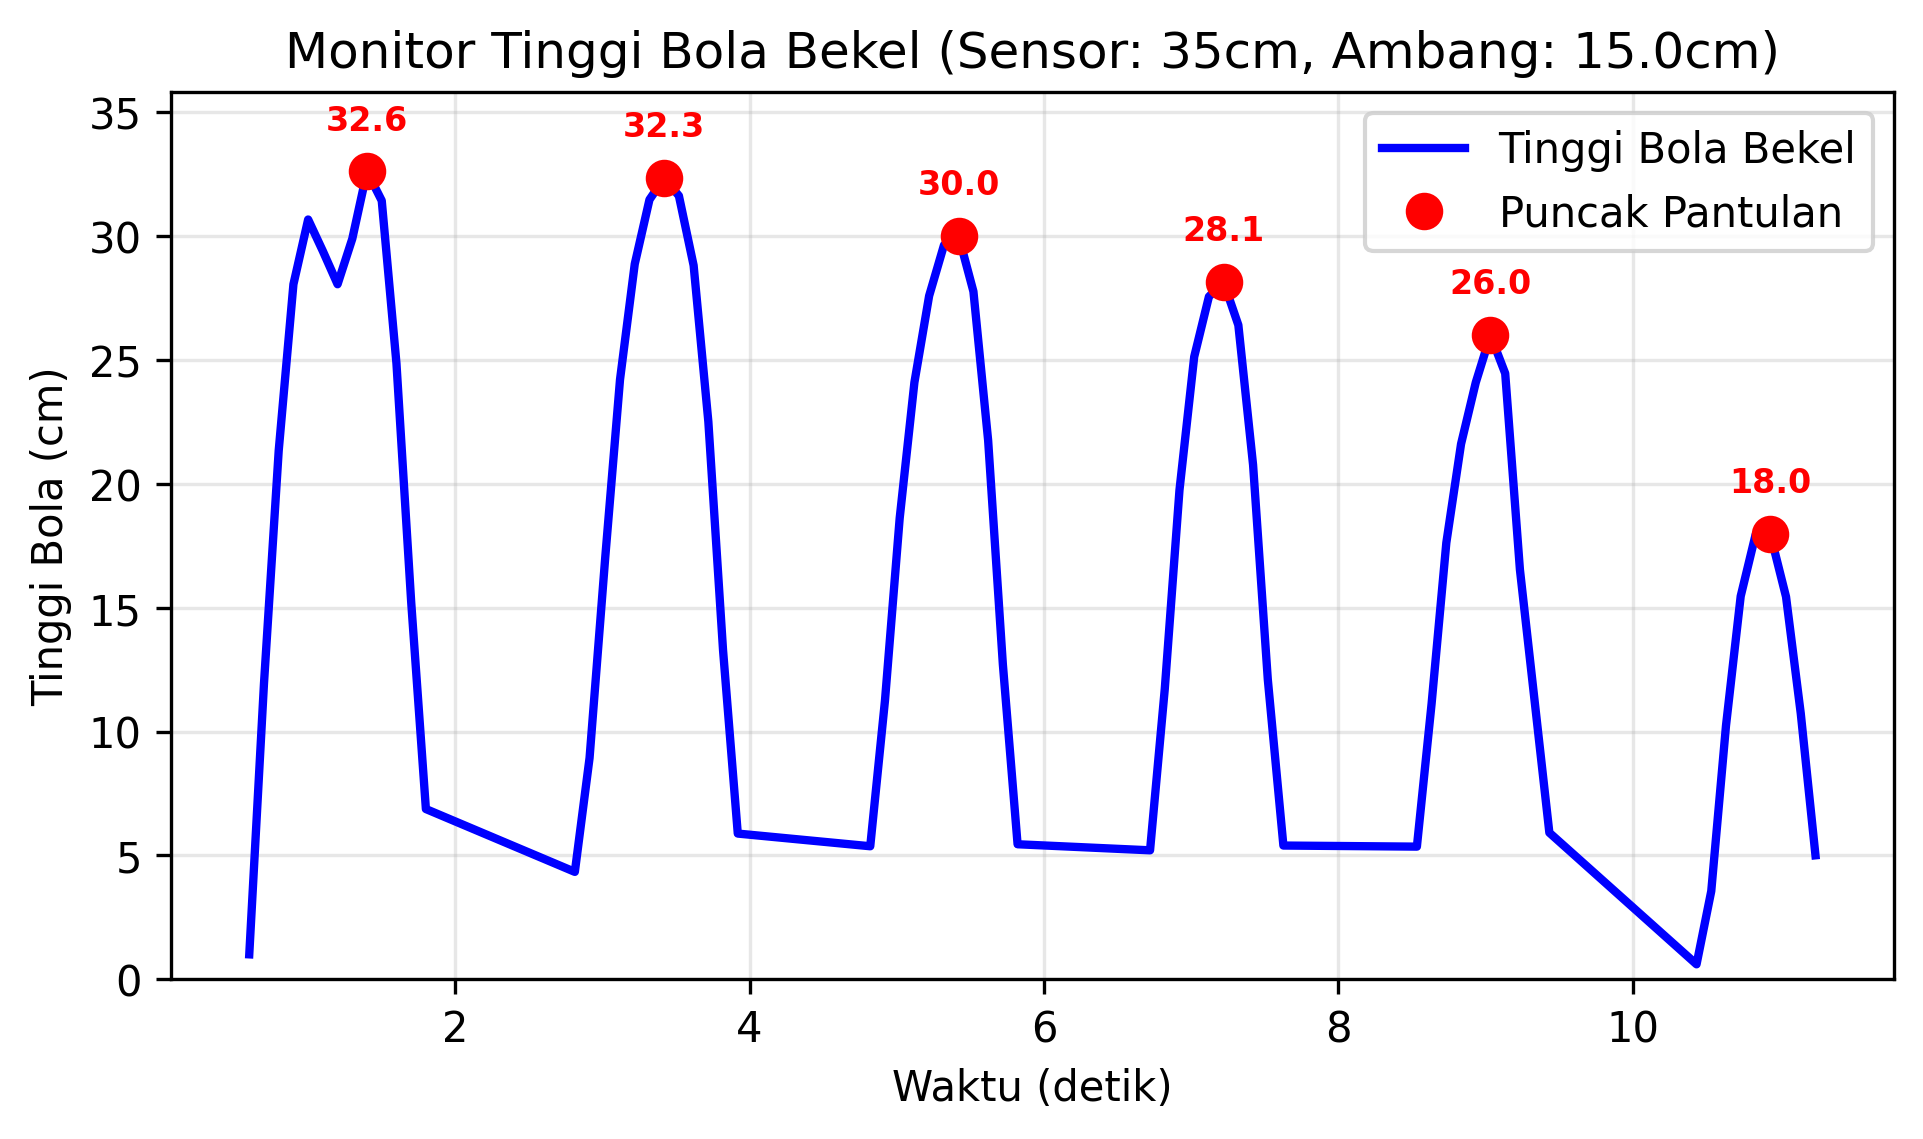
\includegraphics[width=0.5\textwidth]{chapters/DataPercobaan/Grafik_Bola_Bekel_15.png}
    \caption{Grafik Bola Bekel Percobaan 15}
\end{figure}
\begin{figure}[htbp]
    \centering
    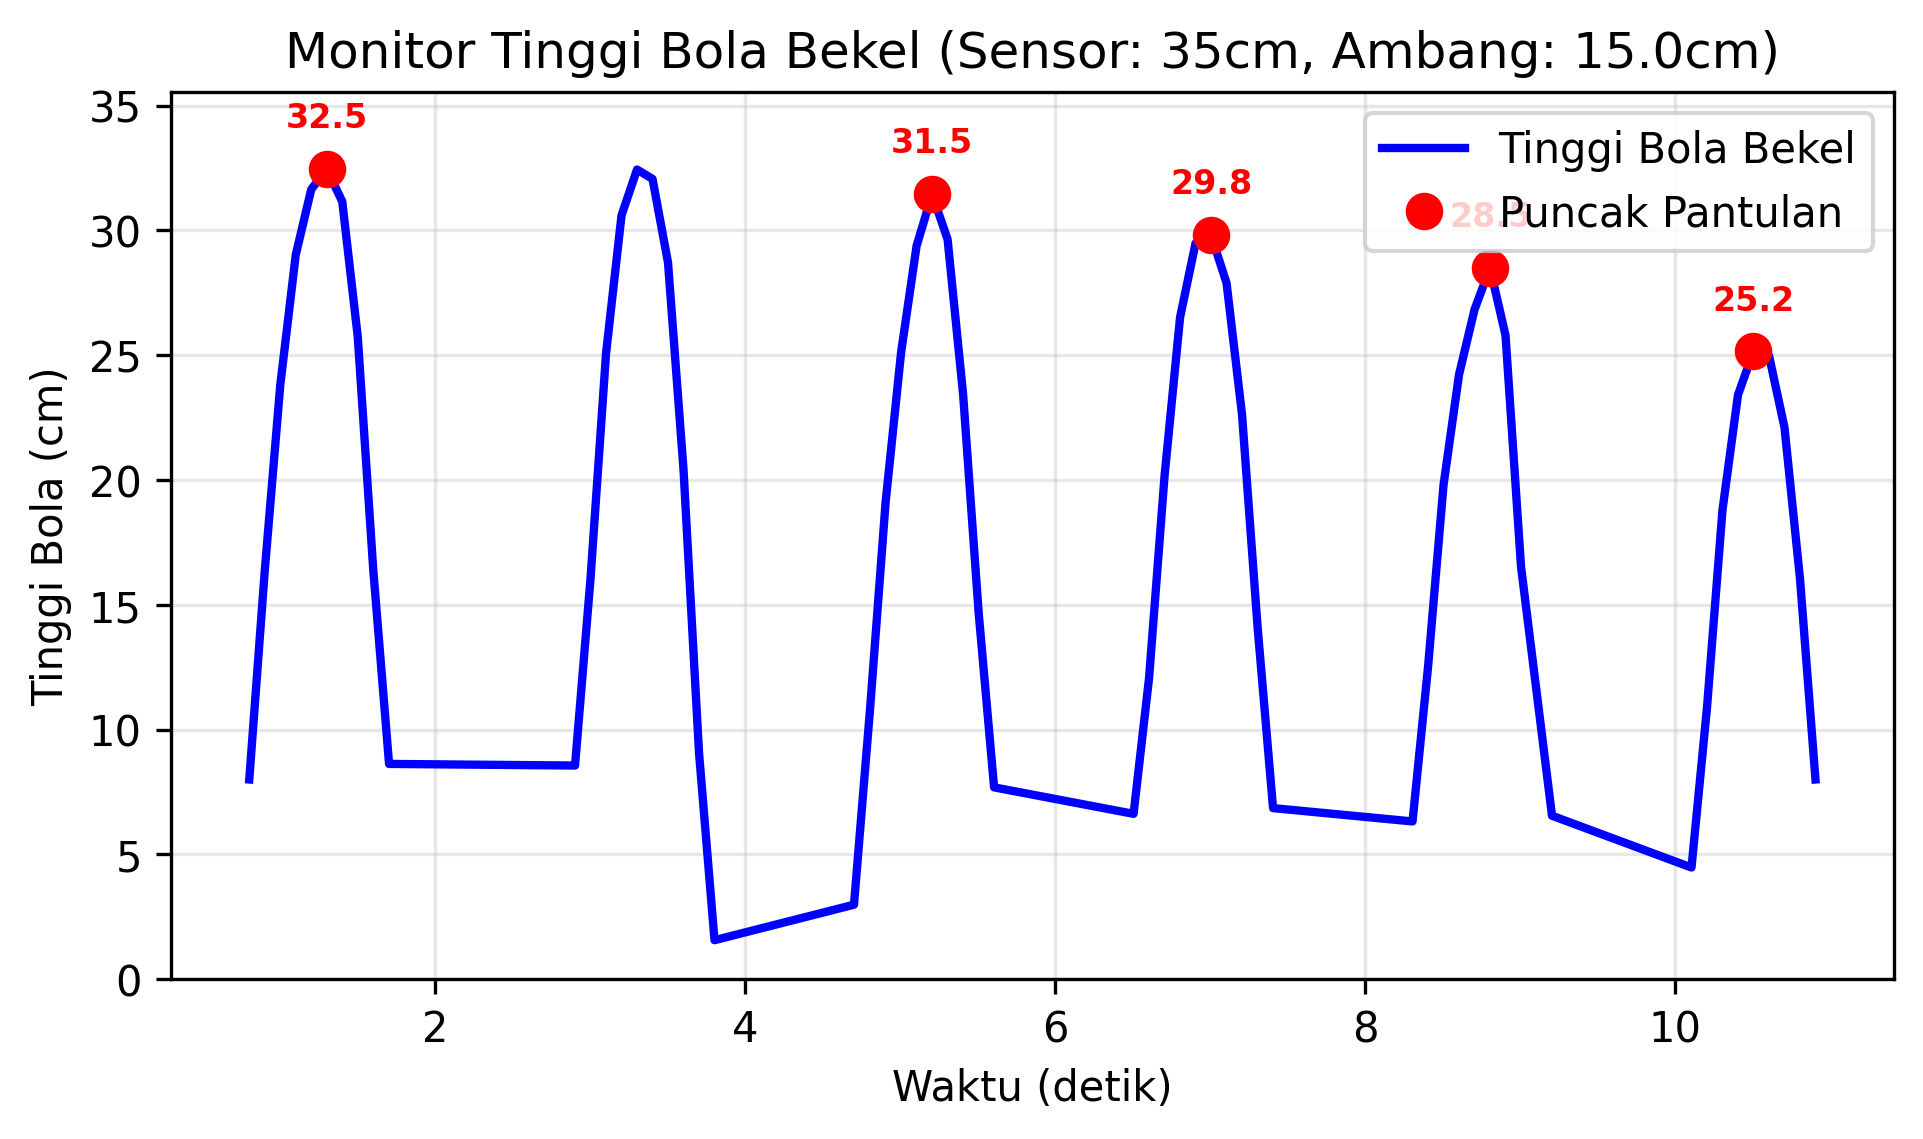
\includegraphics[width=0.5\textwidth]{chapters/DataPercobaan/Grafik_Bola_Bekel_16.png}
    \caption{Grafik Bola Bekel Percobaan 16}
\end{figure}
\begin{figure}[htbp]
    \centering
    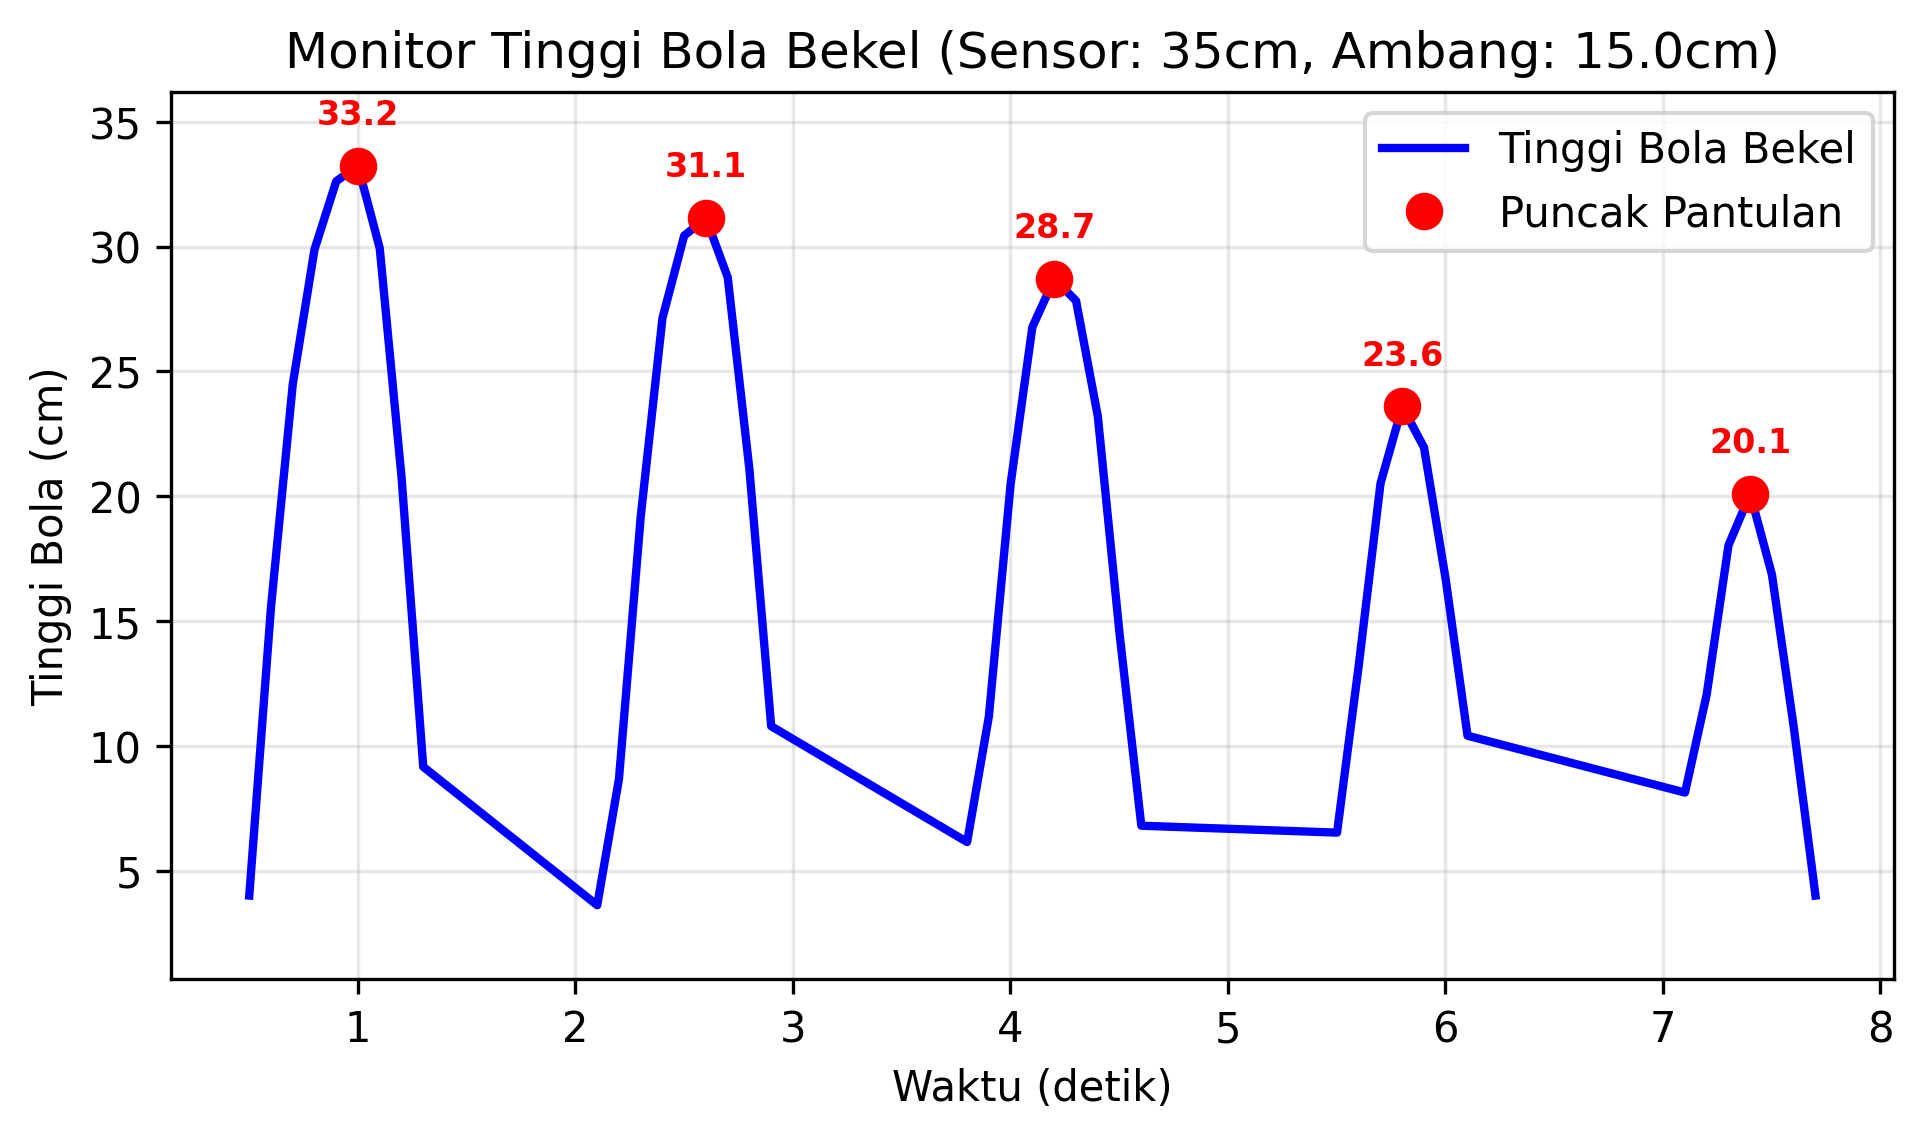
\includegraphics[width=0.5\textwidth]{chapters/DataPercobaan/Grafik_Bola_Bekel_17.png}
    \caption{Grafik Bola Bekel Percobaan 17}
\end{figure}
\begin{figure}[htbp]
    \centering
    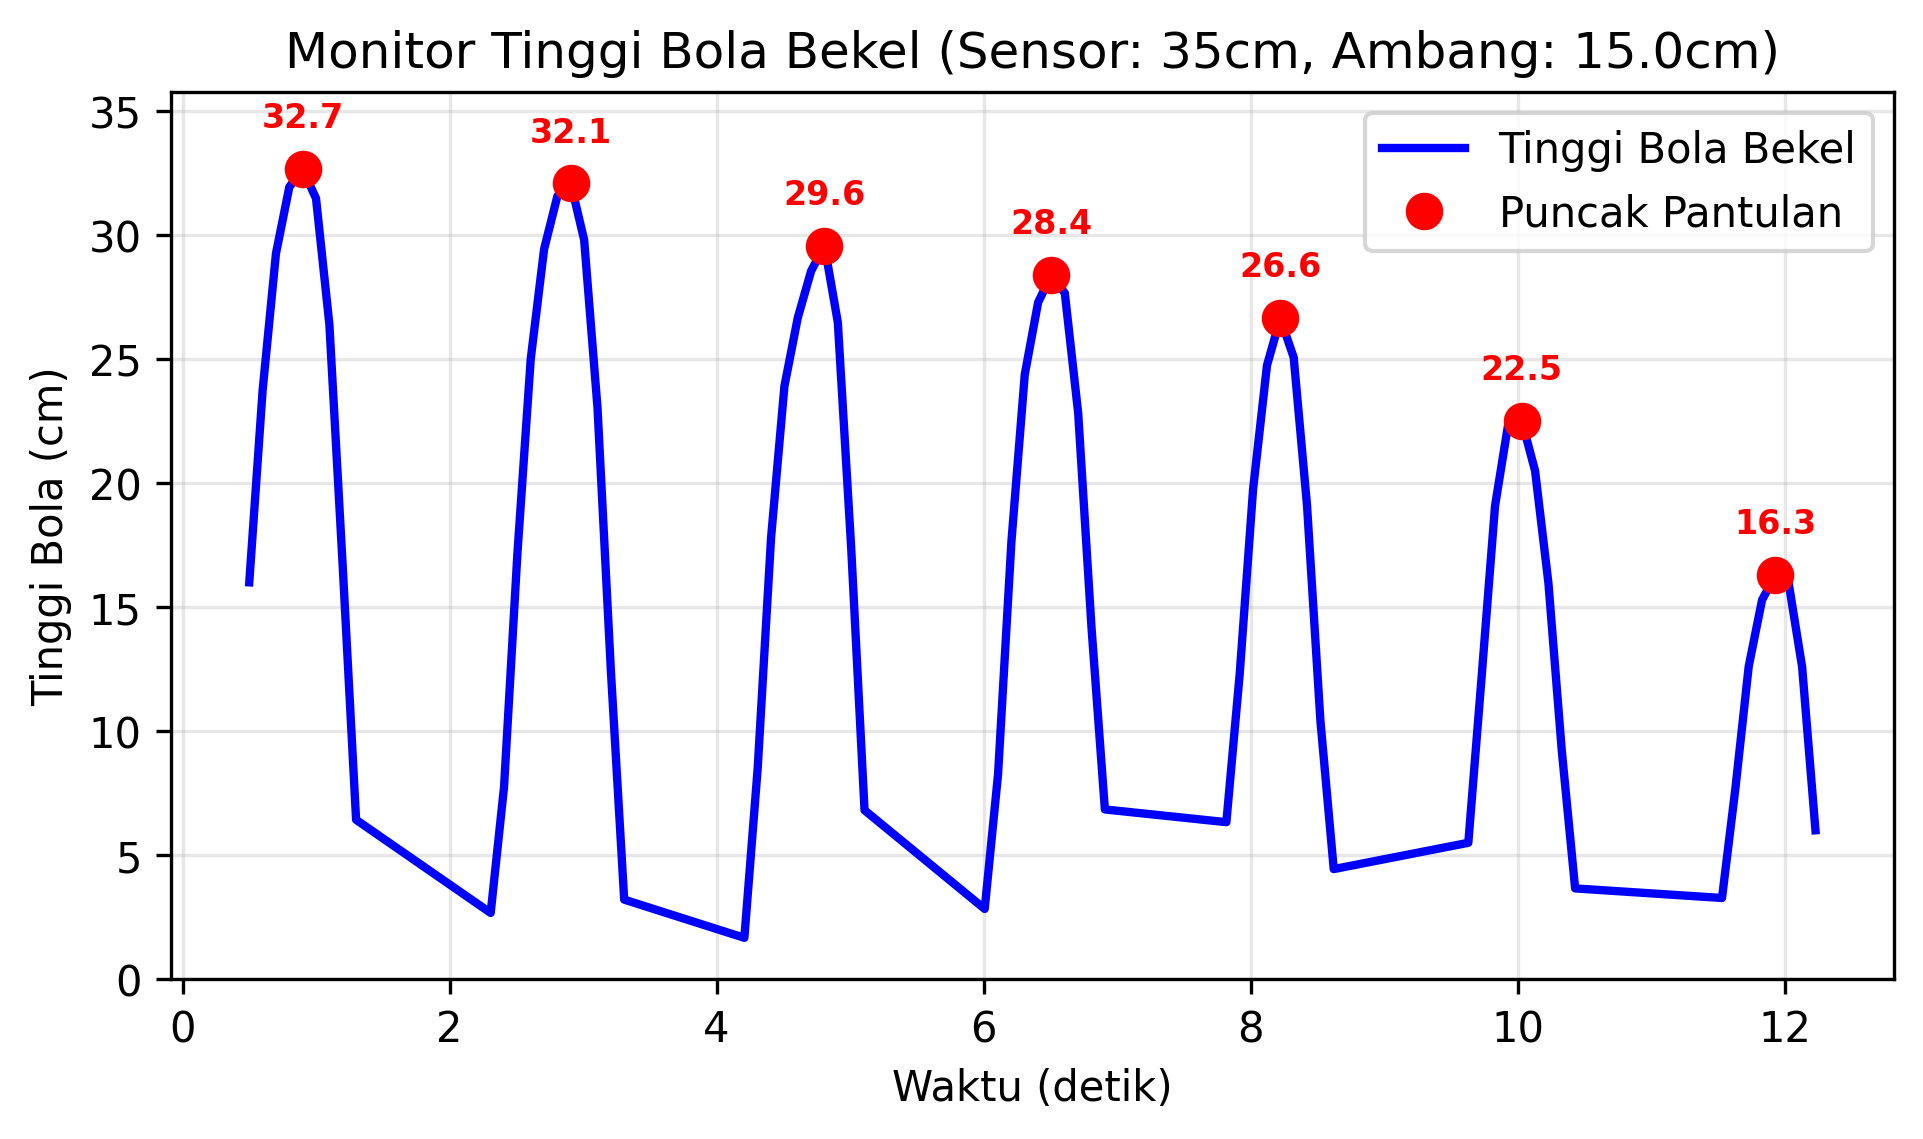
\includegraphics[width=0.5\textwidth]{chapters/DataPercobaan/Grafik_Bola_Bekel_18.png}
    \caption{Grafik Bola Bekel Percobaan 18}
\end{figure}
\begin{figure}[htbp]
    \centering
    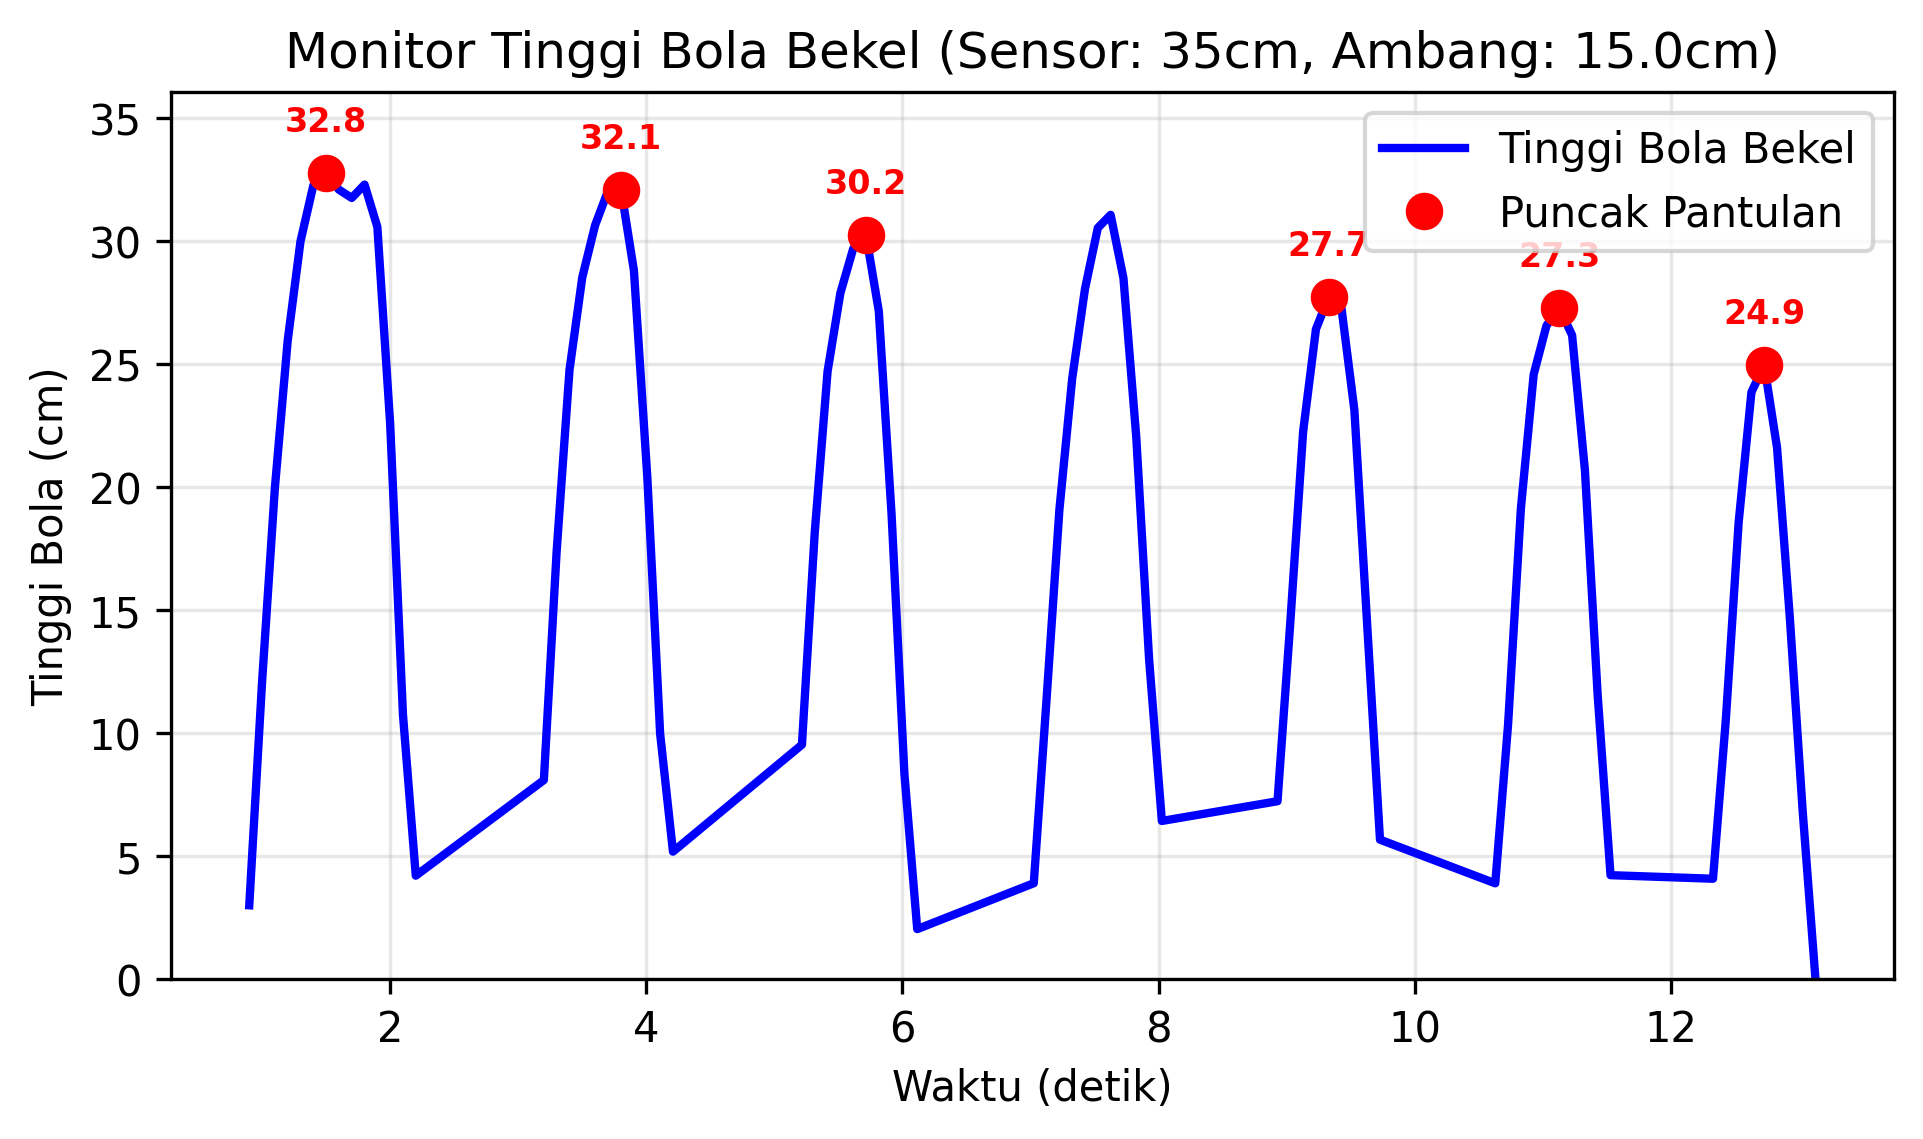
\includegraphics[width=0.5\textwidth]{chapters/DataPercobaan/Grafik_Bola_Bekel_19.png}
    \caption{Grafik Bola Bekel Percobaan 19}
\end{figure}
\begin{figure}[htbp]
    \centering
    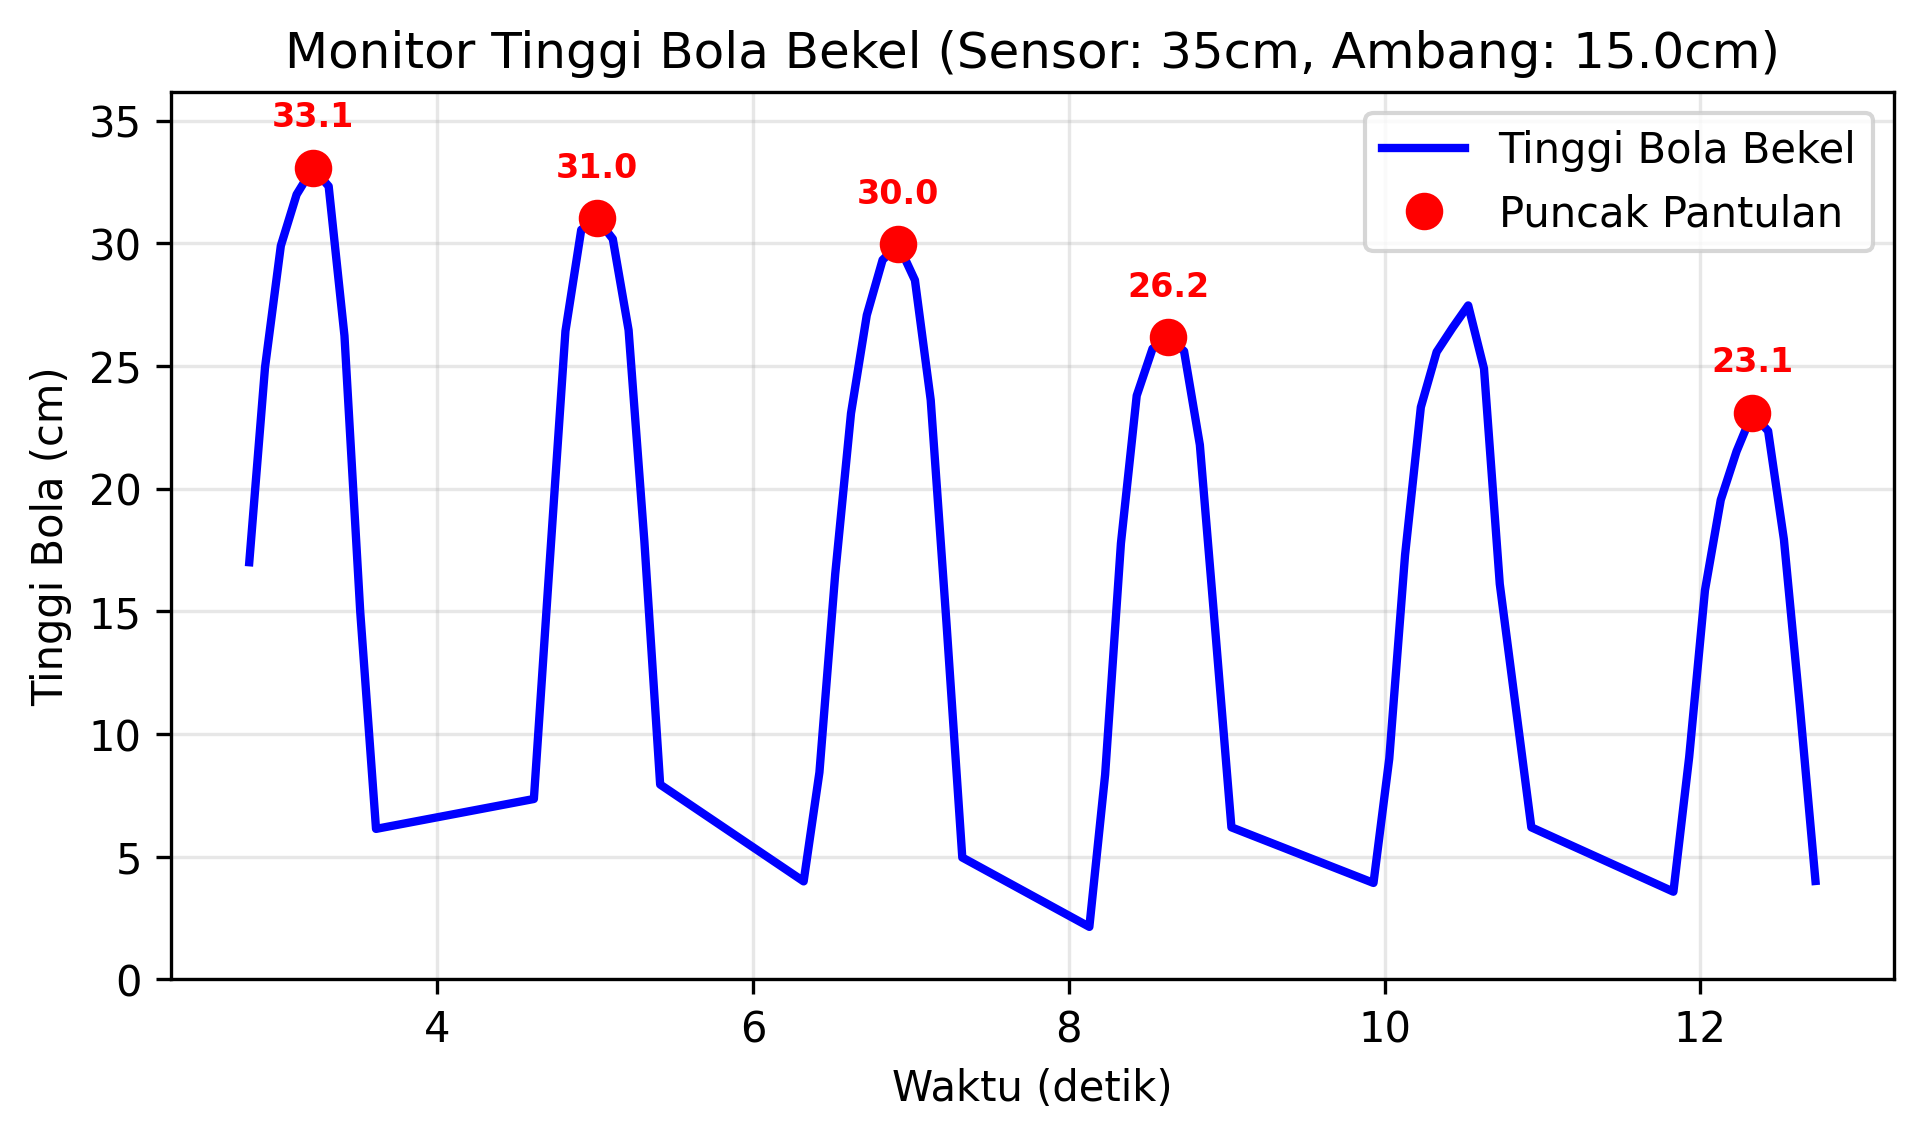
\includegraphics[width=0.5\textwidth]{chapters/DataPercobaan/Grafik_Bola_Bekel_20.png}
    \caption{Grafik Bola Bekel Percobaan 20}
\end{figure}

\section{Bola Tenis Meja}

\subsection{Tabel Percobaan}

\begin{longtable}[htbp]{|c|c|c|}
\caption{Data Bola Tenis Meja 1} \\
\hline
Waktu (detik) & Tinggi Bola Tenis Meja (cm) & Tinggi Sensor (cm) \\ \hline
\endfirsthead
\caption[]{Data Bola Tenis Meja 1} \\
\hline
Waktu (detik) & Tinggi Bola Tenis Meja (cm) & Tinggi Sensor (cm) \\ \hline
\endhead
\multicolumn{3}{r}{Continued on next page} \\
\endfoot
\endlastfoot
0.701000 & 8 & 35 \\ \hline
0.801000 & 18 & 35 \\ \hline
0.901000 & 25 & 35 \\ \hline
1.001000 & 30 & 35 \\ \hline
1.101000 & 32 & 35 \\ \hline
1.201000 & 33 & 35 \\ \hline
1.301000 & 32 & 35 \\ \hline
1.402000 & 32 & 35 \\ \hline
1.502000 & 30 & 35 \\ \hline
1.602000 & 19 & 35 \\ \hline
1.702000 & 10 & 35 \\ \hline
1.802000 & 0 & 35 \\ \hline
2.702000 & 4 & 35 \\ \hline
2.802000 & 10 & 35 \\ \hline
2.902000 & 19 & 35 \\ \hline
3.002000 & 24 & 35 \\ \hline
3.102000 & 28 & 35 \\ \hline
3.202000 & 30 & 35 \\ \hline
3.311000 & 31 & 35 \\ \hline
3.411000 & 30 & 35 \\ \hline
3.511000 & 26 & 35 \\ \hline
3.611000 & 20 & 35 \\ \hline
3.711000 & 12 & 35 \\ \hline
3.811000 & 2 & 35 \\ \hline
4.611000 & 0 & 35 \\ \hline
4.711000 & 8 & 35 \\ \hline
4.811000 & 15 & 35 \\ \hline
4.911000 & 20 & 35 \\ \hline
5.011000 & 23 & 35 \\ \hline
5.111000 & 27 & 35 \\ \hline
5.211000 & 30 & 35 \\ \hline
5.311000 & 30 & 35 \\ \hline
5.412000 & 28 & 35 \\ \hline
5.512000 & 23 & 35 \\ \hline
5.612000 & 15 & 35 \\ \hline
5.712000 & 6 & 35 \\ \hline
6.612000 & 2 & 35 \\ \hline
6.712000 & 6 & 35 \\ \hline
6.812000 & 15 & 35 \\ \hline
6.912000 & 20 & 35 \\ \hline
7.012000 & 24 & 35 \\ \hline
7.112000 & 26 & 35 \\ \hline
7.212000 & 28 & 35 \\ \hline
7.312000 & 28 & 35 \\ \hline
7.412000 & 26 & 35 \\ \hline
7.512000 & 23 & 35 \\ \hline
7.612000 & 17 & 35 \\ \hline
7.712000 & 11 & 35 \\ \hline
8.816000 & 8 & 35 \\ \hline
8.916000 & 14 & 35 \\ \hline
9.016000 & 20 & 35 \\ \hline
9.116000 & 23 & 35 \\ \hline
9.226000 & 24 & 35 \\ \hline
9.326000 & 25 & 35 \\ \hline
9.426000 & 23 & 35 \\ \hline
9.526000 & 19 & 35 \\ \hline
9.626000 & 11 & 35 \\ \hline
9.726000 & 6 & 35 \\ \hline
9.826000 & 0 & 35 \\ \hline
\end{longtable}

\begin{longtable}[htbp]{|c|c|c|}
\caption{Data Bola Tenis Meja 2} \\
\hline
Waktu (detik) & Tinggi Bola Tenis Meja (cm) & Tinggi Sensor (cm) \\ \hline
\endfirsthead
\caption[]{Data Bola Tenis Meja 2} \\
\hline
Waktu (detik) & Tinggi Bola Tenis Meja (cm) & Tinggi Sensor (cm) \\ \hline
\endhead
\multicolumn{3}{r}{Continued on next page} \\
\endfoot
\endlastfoot
1.600000 & 8 & 35 \\ \hline
1.700000 & 17 & 35 \\ \hline
1.800000 & 24 & 35 \\ \hline
1.900000 & 29 & 35 \\ \hline
2.000000 & 32 & 35 \\ \hline
2.100000 & 32 & 35 \\ \hline
2.200000 & 33 & 35 \\ \hline
2.300000 & 32 & 35 \\ \hline
2.400000 & 25 & 35 \\ \hline
2.500000 & 16 & 35 \\ \hline
2.600000 & 6 & 35 \\ \hline
3.600000 & 6 & 35 \\ \hline
3.700000 & 14 & 35 \\ \hline
3.800000 & 21 & 35 \\ \hline
3.900000 & 27 & 35 \\ \hline
4.000000 & 31 & 35 \\ \hline
4.100000 & 32 & 35 \\ \hline
4.200000 & 32 & 35 \\ \hline
4.300000 & 30 & 35 \\ \hline
4.400000 & 25 & 35 \\ \hline
4.500000 & 18 & 35 \\ \hline
4.600000 & 7 & 35 \\ \hline
5.500000 & 0 & 35 \\ \hline
5.600000 & 11 & 35 \\ \hline
5.700000 & 19 & 35 \\ \hline
5.800000 & 24 & 35 \\ \hline
5.900000 & 28 & 35 \\ \hline
6.000000 & 31 & 35 \\ \hline
6.100000 & 31 & 35 \\ \hline
6.200000 & 29 & 35 \\ \hline
6.305000 & 21 & 35 \\ \hline
6.405000 & 15 & 35 \\ \hline
6.514000 & 4 & 35 \\ \hline
7.420000 & 8 & 35 \\ \hline
7.520000 & 14 & 35 \\ \hline
7.620000 & 19 & 35 \\ \hline
7.720000 & 24 & 35 \\ \hline
7.820000 & 26 & 35 \\ \hline
7.920000 & 26 & 35 \\ \hline
8.020000 & 24 & 35 \\ \hline
8.120000 & 20 & 35 \\ \hline
8.220000 & 10 & 35 \\ \hline
8.320000 & 5 & 35 \\ \hline
9.220000 & 0 & 35 \\ \hline
9.320000 & 7 & 35 \\ \hline
9.420000 & 15 & 35 \\ \hline
9.520000 & 19 & 35 \\ \hline
9.620000 & 23 & 35 \\ \hline
9.720000 & 23 & 35 \\ \hline
9.820000 & 19 & 35 \\ \hline
9.920000 & 17 & 35 \\ \hline
10.020000 & 10 & 35 \\ \hline
10.120000 & 3 & 35 \\ \hline
\end{longtable}

\begin{longtable}[htbp]{|c|c|c|}
\caption{Data Bola Tenis Meja 3} \\
\hline
Waktu (detik) & Tinggi Bola Tenis Meja (cm) & Tinggi Sensor (cm) \\ \hline
\endfirsthead
\caption[]{Data Bola Tenis Meja 3} \\
\hline
Waktu (detik) & Tinggi Bola Tenis Meja (cm) & Tinggi Sensor (cm) \\ \hline
\endhead
\multicolumn{3}{r}{Continued on next page} \\
\endfoot
\endlastfoot
0.200000 & 0 & 35 \\ \hline
0.300000 & 10 & 35 \\ \hline
0.400000 & 19 & 35 \\ \hline
0.500000 & 25 & 35 \\ \hline
0.600000 & 27 & 35 \\ \hline
0.700000 & 31 & 35 \\ \hline
0.800000 & 32 & 35 \\ \hline
0.900000 & 33 & 35 \\ \hline
1.000000 & 31 & 35 \\ \hline
1.100000 & 25 & 35 \\ \hline
1.200000 & 15 & 35 \\ \hline
1.300000 & 3 & 35 \\ \hline
2.200000 & 6 & 35 \\ \hline
2.300000 & 15 & 35 \\ \hline
2.401000 & 22 & 35 \\ \hline
2.501000 & 27 & 35 \\ \hline
2.601000 & 30 & 35 \\ \hline
2.701000 & 31 & 35 \\ \hline
2.801000 & 29 & 35 \\ \hline
2.901000 & 24 & 35 \\ \hline
3.001000 & 16 & 35 \\ \hline
3.101000 & 5 & 35 \\ \hline
4.001000 & 4 & 35 \\ \hline
4.101000 & 13 & 35 \\ \hline
4.201000 & 20 & 35 \\ \hline
4.301000 & 26 & 35 \\ \hline
4.401000 & 27 & 35 \\ \hline
4.501000 & 29 & 35 \\ \hline
4.601000 & 27 & 35 \\ \hline
4.701000 & 21 & 35 \\ \hline
4.801000 & 13 & 35 \\ \hline
4.901000 & 2 & 35 \\ \hline
5.805000 & 5 & 35 \\ \hline
5.905000 & 13 & 35 \\ \hline
6.005000 & 20 & 35 \\ \hline
6.105000 & 25 & 35 \\ \hline
6.205000 & 28 & 35 \\ \hline
6.305000 & 29 & 35 \\ \hline
6.405000 & 26 & 35 \\ \hline
6.505000 & 20 & 35 \\ \hline
6.605000 & 15 & 35 \\ \hline
6.705000 & 5 & 35 \\ \hline
7.605000 & 6 & 35 \\ \hline
7.705000 & 13 & 35 \\ \hline
7.805000 & 20 & 35 \\ \hline
7.905000 & 24 & 35 \\ \hline
8.005000 & 26 & 35 \\ \hline
8.105000 & 24 & 35 \\ \hline
8.205000 & 22 & 35 \\ \hline
8.305000 & 16 & 35 \\ \hline
8.405000 & 7 & 35 \\ \hline
9.205000 & 2 & 35 \\ \hline
9.305000 & 6 & 35 \\ \hline
9.405000 & 11 & 35 \\ \hline
9.505000 & 14 & 35 \\ \hline
9.605000 & 16 & 35 \\ \hline
9.705000 & 16 & 35 \\ \hline
9.805000 & 12 & 35 \\ \hline
9.905000 & 6 & 35 \\ \hline
10.005000 & 0 & 35 \\ \hline
\end{longtable}

\begin{longtable}[htbp]{|c|c|c|}
\caption{Data Bola Tenis Meja 4} \\
\hline
Waktu (detik) & Tinggi Bola Tenis Meja (cm) & Tinggi Sensor (cm) \\ \hline
\endfirsthead
\caption[]{Data Bola Tenis Meja 4} \\
\hline
Waktu (detik) & Tinggi Bola Tenis Meja (cm) & Tinggi Sensor (cm) \\ \hline
\endhead
\multicolumn{3}{r}{Continued on next page} \\
\endfoot
\endlastfoot
0.300000 & 6 & 35 \\ \hline
0.400000 & 17 & 35 \\ \hline
0.500000 & 23 & 35 \\ \hline
0.600000 & 28 & 35 \\ \hline
0.700000 & 32 & 35 \\ \hline
0.800000 & 33 & 35 \\ \hline
0.907000 & 33 & 35 \\ \hline
1.007000 & 27 & 35 \\ \hline
1.107000 & 19 & 35 \\ \hline
1.208000 & 6 & 35 \\ \hline
2.018000 & 4 & 35 \\ \hline
2.118000 & 13 & 35 \\ \hline
2.218000 & 20 & 35 \\ \hline
2.318000 & 26 & 35 \\ \hline
2.418000 & 31 & 35 \\ \hline
2.518000 & 32 & 35 \\ \hline
2.618000 & 31 & 35 \\ \hline
2.718000 & 28 & 35 \\ \hline
2.826000 & 20 & 35 \\ \hline
2.926000 & 9 & 35 \\ \hline
3.026000 & 3 & 35 \\ \hline
3.926000 & 11 & 35 \\ \hline
4.026000 & 18 & 35 \\ \hline
4.126000 & 23 & 35 \\ \hline
4.226000 & 28 & 35 \\ \hline
4.326000 & 31 & 35 \\ \hline
4.426000 & 30 & 35 \\ \hline
4.526000 & 26 & 35 \\ \hline
4.626000 & 21 & 35 \\ \hline
4.726000 & 10 & 35 \\ \hline
4.826000 & 2 & 35 \\ \hline
5.726000 & 13 & 35 \\ \hline
5.826000 & 20 & 35 \\ \hline
5.926000 & 23 & 35 \\ \hline
6.026000 & 24 & 35 \\ \hline
6.126000 & 25 & 35 \\ \hline
6.226000 & 25 & 35 \\ \hline
6.326000 & 22 & 35 \\ \hline
6.426000 & 15 & 35 \\ \hline
6.526000 & 6 & 35 \\ \hline
7.426000 & 3 & 35 \\ \hline
7.526000 & 10 & 35 \\ \hline
7.626000 & 17 & 35 \\ \hline
7.726000 & 20 & 35 \\ \hline
7.826000 & 20 & 35 \\ \hline
7.926000 & 20 & 35 \\ \hline
8.026000 & 18 & 35 \\ \hline
8.126000 & 10 & 35 \\ \hline
8.226000 & 3 & 35 \\ \hline
9.133000 & 2 & 35 \\ \hline
9.233000 & 10 & 35 \\ \hline
9.333000 & 15 & 35 \\ \hline
9.433000 & 19 & 35 \\ \hline
9.540000 & 20 & 35 \\ \hline
9.640000 & 18 & 35 \\ \hline
9.740000 & 14 & 35 \\ \hline
9.840000 & 6 & 35 \\ \hline
\end{longtable}

\begin{longtable}[htbp]{|c|c|c|}
\caption{Data Bola Tenis Meja 5} \\
\hline
Waktu (detik) & Tinggi Bola Tenis Meja (cm) & Tinggi Sensor (cm) \\ \hline
\endfirsthead
\caption[]{Data Bola Tenis Meja 5} \\
\hline
Waktu (detik) & Tinggi Bola Tenis Meja (cm) & Tinggi Sensor (cm) \\ \hline
\endhead
\multicolumn{3}{r}{Continued on next page} \\
\endfoot
\endlastfoot
0.510000 & 13 & 35 \\ \hline
0.610000 & 21 & 35 \\ \hline
0.710000 & 29 & 35 \\ \hline
0.810000 & 33 & 35 \\ \hline
0.910000 & 33 & 35 \\ \hline
1.010000 & 30 & 35 \\ \hline
1.110000 & 22 & 35 \\ \hline
1.210000 & 12 & 35 \\ \hline
1.310000 & 3 & 35 \\ \hline
2.110000 & 0 & 35 \\ \hline
2.210000 & 5 & 35 \\ \hline
2.310000 & 18 & 35 \\ \hline
2.410000 & 24 & 35 \\ \hline
2.510000 & 29 & 35 \\ \hline
2.610000 & 30 & 35 \\ \hline
2.710000 & 26 & 35 \\ \hline
2.810000 & 22 & 35 \\ \hline
2.910000 & 13 & 35 \\ \hline
3.010000 & 4 & 35 \\ \hline
3.910000 & 9 & 35 \\ \hline
4.010000 & 16 & 35 \\ \hline
4.110000 & 23 & 35 \\ \hline
4.210000 & 27 & 35 \\ \hline
4.310000 & 27 & 35 \\ \hline
4.410000 & 25 & 35 \\ \hline
4.510000 & 18 & 35 \\ \hline
4.610000 & 11 & 35 \\ \hline
4.710000 & 2 & 35 \\ \hline
5.610000 & 6 & 35 \\ \hline
5.710000 & 15 & 35 \\ \hline
5.810000 & 21 & 35 \\ \hline
5.910000 & 26 & 35 \\ \hline
6.010000 & 27 & 35 \\ \hline
6.110000 & 25 & 35 \\ \hline
6.210000 & 20 & 35 \\ \hline
6.310000 & 14 & 35 \\ \hline
6.410000 & 4 & 35 \\ \hline
7.210000 & 0 & 35 \\ \hline
7.310000 & 6 & 35 \\ \hline
7.410000 & 16 & 35 \\ \hline
7.510000 & 22 & 35 \\ \hline
7.610000 & 25 & 35 \\ \hline
7.710000 & 28 & 35 \\ \hline
7.810000 & 27 & 35 \\ \hline
7.910000 & 22 & 35 \\ \hline
8.010000 & 15 & 35 \\ \hline
8.110000 & 6 & 35 \\ \hline
9.010000 & 8 & 35 \\ \hline
9.110000 & 17 & 35 \\ \hline
9.210000 & 22 & 35 \\ \hline
9.310000 & 26 & 35 \\ \hline
9.410000 & 26 & 35 \\ \hline
9.510000 & 23 & 35 \\ \hline
9.610000 & 19 & 35 \\ \hline
9.710000 & 13 & 35 \\ \hline
9.810000 & 5 & 35 \\ \hline
10.713000 & 2 & 35 \\ \hline
10.813000 & 9 & 35 \\ \hline
10.913000 & 12 & 35 \\ \hline
11.013000 & 13 & 35 \\ \hline
\end{longtable}

\begin{longtable}[htbp]{|c|c|c|}
\caption{Data Bola Tenis Meja 6} \\
\hline
Waktu (detik) & Tinggi Bola Tenis Meja (cm) & Tinggi Sensor (cm) \\ \hline
\endfirsthead
\caption[]{Data Bola Tenis Meja 6} \\
\hline
Waktu (detik) & Tinggi Bola Tenis Meja (cm) & Tinggi Sensor (cm) \\ \hline
\endhead
\multicolumn{3}{r}{Continued on next page} \\
\endfoot
\endlastfoot
0.600000 & 4 & 35 \\ \hline
0.700000 & 14 & 35 \\ \hline
0.800000 & 23 & 35 \\ \hline
0.900000 & 29 & 35 \\ \hline
1.000000 & 32 & 35 \\ \hline
1.100000 & 32 & 35 \\ \hline
1.200000 & 33 & 35 \\ \hline
1.300000 & 32 & 35 \\ \hline
1.400000 & 26 & 35 \\ \hline
1.500000 & 13 & 35 \\ \hline
1.600000 & 3 & 35 \\ \hline
2.500000 & 6 & 35 \\ \hline
2.700000 & 22 & 35 \\ \hline
2.800000 & 28 & 35 \\ \hline
2.900000 & 31 & 35 \\ \hline
3.000000 & 31 & 35 \\ \hline
3.100000 & 26 & 35 \\ \hline
3.200000 & 20 & 35 \\ \hline
3.300000 & 11 & 35 \\ \hline
3.400000 & 3 & 35 \\ \hline
4.300000 & 6 & 35 \\ \hline
4.400000 & 15 & 35 \\ \hline
4.500000 & 22 & 35 \\ \hline
4.600000 & 28 & 35 \\ \hline
4.700000 & 30 & 35 \\ \hline
4.800000 & 28 & 35 \\ \hline
4.900000 & 22 & 35 \\ \hline
5.000000 & 17 & 35 \\ \hline
5.100000 & 8 & 35 \\ \hline
5.901000 & 4 & 35 \\ \hline
6.001000 & 12 & 35 \\ \hline
6.101000 & 19 & 35 \\ \hline
6.201000 & 25 & 35 \\ \hline
6.301000 & 30 & 35 \\ \hline
6.401000 & 31 & 35 \\ \hline
6.501000 & 28 & 35 \\ \hline
6.601000 & 22 & 35 \\ \hline
6.701000 & 13 & 35 \\ \hline
6.801000 & 5 & 35 \\ \hline
7.501000 & 0 & 35 \\ \hline
7.601000 & 8 & 35 \\ \hline
7.701000 & 16 & 35 \\ \hline
7.801000 & 21 & 35 \\ \hline
7.901000 & 26 & 35 \\ \hline
8.001000 & 28 & 35 \\ \hline
8.101000 & 25 & 35 \\ \hline
8.203000 & 20 & 35 \\ \hline
8.303000 & 14 & 35 \\ \hline
8.403000 & 4 & 35 \\ \hline
9.209000 & 2 & 35 \\ \hline
9.309000 & 8 & 35 \\ \hline
9.409000 & 18 & 35 \\ \hline
9.509000 & 6 & 35 \\ \hline
9.609000 & 27 & 35 \\ \hline
9.709000 & 26 & 35 \\ \hline
9.809000 & 24 & 35 \\ \hline
9.909000 & 19 & 35 \\ \hline
10.009000 & 9 & 35 \\ \hline
10.109000 & 0 & 35 \\ \hline
10.821000 & 3 & 35 \\ \hline
11.121000 & 20 & 35 \\ \hline
11.221000 & 23 & 35 \\ \hline
11.321000 & 25 & 35 \\ \hline
11.421000 & 22 & 35 \\ \hline
11.521000 & 17 & 35 \\ \hline
11.625000 & 8 & 35 \\ \hline
11.725000 & 1 & 35 \\ \hline
\end{longtable}

\begin{longtable}[htbp]{|c|c|c|}
\caption{Data Bola Tenis Meja 7} \\
\hline
Waktu (detik) & Tinggi Bola Tenis Meja (cm) & Tinggi Sensor (cm) \\ \hline
\endfirsthead
\caption[]{Data Bola Tenis Meja 7} \\
\hline
Waktu (detik) & Tinggi Bola Tenis Meja (cm) & Tinggi Sensor (cm) \\ \hline
\endhead
\multicolumn{3}{r}{Continued on next page} \\
\endfoot
\endlastfoot
0.300000 & 8 & 35 \\ \hline
0.400000 & 19 & 35 \\ \hline
0.500000 & 26 & 35 \\ \hline
0.600000 & 31 & 35 \\ \hline
0.700000 & 33 & 35 \\ \hline
0.800000 & 33 & 35 \\ \hline
0.900000 & 30 & 35 \\ \hline
1.000000 & 21 & 35 \\ \hline
1.100000 & 9 & 35 \\ \hline
2.000000 & 0 & 35 \\ \hline
2.100000 & 9 & 35 \\ \hline
2.200000 & 18 & 35 \\ \hline
2.300000 & 24 & 35 \\ \hline
2.400000 & 29 & 35 \\ \hline
2.500000 & 32 & 35 \\ \hline
2.600000 & 31 & 35 \\ \hline
2.700000 & 27 & 35 \\ \hline
2.800000 & 19 & 35 \\ \hline
2.900000 & 10 & 35 \\ \hline
3.000000 & 0 & 35 \\ \hline
3.709000 & 0 & 35 \\ \hline
3.809000 & 9 & 35 \\ \hline
3.909000 & 17 & 35 \\ \hline
4.009000 & 23 & 35 \\ \hline
4.109000 & 27 & 35 \\ \hline
4.209000 & 30 & 35 \\ \hline
4.309000 & 29 & 35 \\ \hline
4.417000 & 24 & 35 \\ \hline
4.517000 & 18 & 35 \\ \hline
4.617000 & 7 & 35 \\ \hline
5.417000 & 4 & 35 \\ \hline
5.517000 & 13 & 35 \\ \hline
5.617000 & 19 & 35 \\ \hline
5.717000 & 24 & 35 \\ \hline
5.817000 & 25 & 35 \\ \hline
5.917000 & 24 & 35 \\ \hline
6.017000 & 19 & 35 \\ \hline
6.117000 & 13 & 35 \\ \hline
6.217000 & 3 & 35 \\ \hline
7.117000 & 1 & 35 \\ \hline
7.217000 & 8 & 35 \\ \hline
7.317000 & 16 & 35 \\ \hline
7.417000 & 20 & 35 \\ \hline
7.517000 & 22 & 35 \\ \hline
7.624000 & 22 & 35 \\ \hline
7.724000 & 19 & 35 \\ \hline
7.824000 & 11 & 35 \\ \hline
7.924000 & 1 & 35 \\ \hline
8.824000 & 4 & 35 \\ \hline
8.924000 & 10 & 35 \\ \hline
9.024000 & 15 & 35 \\ \hline
9.126000 & 18 & 35 \\ \hline
9.226000 & 18 & 35 \\ \hline
9.326000 & 18 & 35 \\ \hline
9.535000 & 2 & 35 \\ \hline
\end{longtable}

\begin{longtable}[htbp]{|c|c|c|}
\caption{Data Bola Tenis Meja 8} \\
\hline
Waktu (detik) & Tinggi Bola Tenis Meja (cm) & Tinggi Sensor (cm) \\ \hline
\endfirsthead
\caption[]{Data Bola Tenis Meja 8} \\
\hline
Waktu (detik) & Tinggi Bola Tenis Meja (cm) & Tinggi Sensor (cm) \\ \hline
\endhead
\multicolumn{3}{r}{Continued on next page} \\
\endfoot
\endlastfoot
0.500000 & 5 & 35 \\ \hline
0.600000 & 16 & 35 \\ \hline
0.700000 & 25 & 35 \\ \hline
0.800000 & 30 & 35 \\ \hline
0.900000 & 32 & 35 \\ \hline
1.000000 & 33 & 35 \\ \hline
1.100000 & 32 & 35 \\ \hline
1.200000 & 28 & 35 \\ \hline
1.300000 & 19 & 35 \\ \hline
1.400000 & 5 & 35 \\ \hline
2.300000 & 6 & 35 \\ \hline
2.400000 & 14 & 35 \\ \hline
2.500000 & 22 & 35 \\ \hline
2.600000 & 28 & 35 \\ \hline
2.700000 & 31 & 35 \\ \hline
2.800000 & 32 & 35 \\ \hline
2.900000 & 31 & 35 \\ \hline
3.000000 & 27 & 35 \\ \hline
3.101000 & 19 & 35 \\ \hline
3.201000 & 6 & 35 \\ \hline
3.301000 & 0 & 35 \\ \hline
4.101000 & 1 & 35 \\ \hline
4.201000 & 12 & 35 \\ \hline
4.301000 & 19 & 35 \\ \hline
4.401000 & 25 & 35 \\ \hline
4.501000 & 28 & 35 \\ \hline
4.601000 & 29 & 35 \\ \hline
4.709000 & 27 & 35 \\ \hline
4.809000 & 22 & 35 \\ \hline
4.909000 & 15 & 35 \\ \hline
5.009000 & 4 & 35 \\ \hline
5.709000 & 2 & 35 \\ \hline
5.809000 & 9 & 35 \\ \hline
5.909000 & 15 & 35 \\ \hline
6.009000 & 20 & 35 \\ \hline
6.109000 & 25 & 35 \\ \hline
6.210000 & 27 & 35 \\ \hline
6.310000 & 26 & 35 \\ \hline
6.410000 & 24 & 35 \\ \hline
6.510000 & 18 & 35 \\ \hline
6.610000 & 8 & 35 \\ \hline
6.710000 & 0 & 35 \\ \hline
7.416000 & 5 & 35 \\ \hline
7.516000 & 13 & 35 \\ \hline
7.616000 & 19 & 35 \\ \hline
7.716000 & 22 & 35 \\ \hline
7.816000 & 19 & 35 \\ \hline
7.916000 & 17 & 35 \\ \hline
8.016000 & 9 & 35 \\ \hline
8.817000 & 4 & 35 \\ \hline
8.917000 & 9 & 35 \\ \hline
9.118000 & 19 & 35 \\ \hline
9.218000 & 19 & 35 \\ \hline
9.318000 & 13 & 35 \\ \hline
9.418000 & 5 & 35 \\ \hline
\end{longtable}

\begin{longtable}[htbp]{|c|c|c|}
\caption{Data Bola Tenis Meja 9} \\
\hline
Waktu (detik) & Tinggi Bola Tenis Meja (cm) & Tinggi Sensor (cm) \\ \hline
\endfirsthead
\caption[]{Data Bola Tenis Meja 9} \\
\hline
Waktu (detik) & Tinggi Bola Tenis Meja (cm) & Tinggi Sensor (cm) \\ \hline
\endhead
\multicolumn{3}{r}{Continued on next page} \\
\endfoot
\endlastfoot
0.560302 & 6 & 35 \\ \hline
0.100000 & 18 & 35 \\ \hline
0.200000 & 25 & 35 \\ \hline
0.300000 & 29 & 35 \\ \hline
0.400000 & 32 & 35 \\ \hline
0.500000 & 33 & 35 \\ \hline
0.600000 & 32 & 35 \\ \hline
0.700000 & 29 & 35 \\ \hline
0.800000 & 19 & 35 \\ \hline
0.900000 & 10 & 35 \\ \hline
1.801000 & 6 & 35 \\ \hline
1.902000 & 14 & 35 \\ \hline
2.002000 & 20 & 35 \\ \hline
2.102000 & 26 & 35 \\ \hline
2.202000 & 30 & 35 \\ \hline
2.302000 & 31 & 35 \\ \hline
2.402000 & 30 & 35 \\ \hline
2.504000 & 24 & 35 \\ \hline
2.604000 & 18 & 35 \\ \hline
2.704000 & 9 & 35 \\ \hline
3.604000 & 4 & 35 \\ \hline
3.704000 & 11 & 35 \\ \hline
3.804000 & 16 & 35 \\ \hline
3.904000 & 22 & 35 \\ \hline
4.004000 & 27 & 35 \\ \hline
4.105000 & 29 & 35 \\ \hline
4.205000 & 27 & 35 \\ \hline
4.305000 & 22 & 35 \\ \hline
4.405000 & 15 & 35 \\ \hline
4.505000 & 5 & 35 \\ \hline
5.305000 & 2 & 35 \\ \hline
5.405000 & 9 & 35 \\ \hline
5.505000 & 16 & 35 \\ \hline
5.605000 & 23 & 35 \\ \hline
5.705000 & 25 & 35 \\ \hline
5.805000 & 27 & 35 \\ \hline
5.905000 & 22 & 35 \\ \hline
6.005000 & 19 & 35 \\ \hline
6.105000 & 12 & 35 \\ \hline
6.205000 & 3 & 35 \\ \hline
7.005000 & 5 & 35 \\ \hline
7.105000 & 12 & 35 \\ \hline
7.205000 & 19 & 35 \\ \hline
7.305000 & 23 & 35 \\ \hline
7.405000 & 26 & 35 \\ \hline
7.505000 & 27 & 35 \\ \hline
7.605000 & 24 & 35 \\ \hline
7.705000 & 20 & 35 \\ \hline
7.805000 & 11 & 35 \\ \hline
7.905000 & 2 & 35 \\ \hline
8.605000 & 2 & 35 \\ \hline
8.705000 & 6 & 35 \\ \hline
8.805000 & 11 & 35 \\ \hline
8.905000 & 10 & 35 \\ \hline
\end{longtable}

\begin{longtable}[htbp]{|c|c|c|}
\caption{Data Bola Tenis Meja 10} \\
\hline
Waktu (detik) & Tinggi Bola Tenis Meja (cm) & Tinggi Sensor (cm) \\ \hline
\endfirsthead
\caption[]{Data Bola Tenis Meja 10} \\
\hline
Waktu (detik) & Tinggi Bola Tenis Meja (cm) & Tinggi Sensor (cm) \\ \hline
\endhead
\multicolumn{3}{r}{Continued on next page} \\
\endfoot
\endlastfoot
0.401000 & 6 & 35 \\ \hline
0.501000 & 16 & 35 \\ \hline
0.601000 & 23 & 35 \\ \hline
0.701000 & 27 & 35 \\ \hline
0.801000 & 31 & 35 \\ \hline
0.901000 & 33 & 35 \\ \hline
1.001000 & 33 & 35 \\ \hline
1.101000 & 31 & 35 \\ \hline
1.201000 & 23 & 35 \\ \hline
1.301000 & 14 & 35 \\ \hline
1.401000 & 2 & 35 \\ \hline
2.303000 & 8 & 35 \\ \hline
2.403000 & 19 & 35 \\ \hline
2.503000 & 24 & 35 \\ \hline
2.603000 & 29 & 35 \\ \hline
2.703000 & 31 & 35 \\ \hline
2.803000 & 33 & 35 \\ \hline
2.903000 & 31 & 35 \\ \hline
3.003000 & 26 & 35 \\ \hline
3.103000 & 17 & 35 \\ \hline
3.203000 & 7 & 35 \\ \hline
4.103000 & 7 & 35 \\ \hline
4.203000 & 14 & 35 \\ \hline
4.303000 & 22 & 35 \\ \hline
4.403000 & 26 & 35 \\ \hline
4.503000 & 29 & 35 \\ \hline
4.603000 & 30 & 35 \\ \hline
4.703000 & 27 & 35 \\ \hline
4.803000 & 21 & 35 \\ \hline
4.903000 & 13 & 35 \\ \hline
5.003000 & 3 & 35 \\ \hline
5.803000 & 6 & 35 \\ \hline
5.903000 & 16 & 35 \\ \hline
6.003000 & 19 & 35 \\ \hline
6.103000 & 25 & 35 \\ \hline
6.203000 & 27 & 35 \\ \hline
6.303000 & 27 & 35 \\ \hline
6.403000 & 24 & 35 \\ \hline
6.503000 & 17 & 35 \\ \hline
6.603000 & 8 & 35 \\ \hline
6.703000 & 0 & 35 \\ \hline
7.503000 & 6 & 35 \\ \hline
7.603000 & 14 & 35 \\ \hline
7.703000 & 21 & 35 \\ \hline
7.803000 & 26 & 35 \\ \hline
7.903000 & 25 & 35 \\ \hline
8.003000 & 21 & 35 \\ \hline
8.111000 & 13 & 35 \\ \hline
8.211000 & 5 & 35 \\ \hline
\end{longtable}

\begin{longtable}[htbp]{|c|c|c|}
\caption{Data Bola Tenis Meja 11} \\
\hline
Waktu (detik) & Tinggi Bola Tenis Meja (cm) & Tinggi Sensor (cm) \\ \hline
\endfirsthead
\caption[]{Data Bola Tenis Meja 11} \\
\hline
Waktu (detik) & Tinggi Bola Tenis Meja (cm) & Tinggi Sensor (cm) \\ \hline
\endhead
\multicolumn{3}{r}{Continued on next page} \\
\endfoot
\endlastfoot
0.200000 & 6 & 35 \\ \hline
0.300000 & 18 & 35 \\ \hline
0.400000 & 25 & 35 \\ \hline
0.500000 & 30 & 35 \\ \hline
0.600000 & 33 & 35 \\ \hline
0.800000 & 32 & 35 \\ \hline
0.900000 & 28 & 35 \\ \hline
1.000000 & 18 & 35 \\ \hline
1.100000 & 6 & 35 \\ \hline
1.900000 & 4 & 35 \\ \hline
2.000000 & 13 & 35 \\ \hline
2.100000 & 20 & 35 \\ \hline
2.200000 & 25 & 35 \\ \hline
2.300000 & 30 & 35 \\ \hline
2.400000 & 32 & 35 \\ \hline
2.500000 & 31 & 35 \\ \hline
2.600000 & 26 & 35 \\ \hline
2.700000 & 20 & 35 \\ \hline
2.800000 & 11 & 35 \\ \hline
2.901000 & 0 & 35 \\ \hline
3.601000 & 0 & 35 \\ \hline
3.701000 & 10 & 35 \\ \hline
3.801000 & 18 & 35 \\ \hline
3.901000 & 22 & 35 \\ \hline
4.001000 & 26 & 35 \\ \hline
4.101000 & 28 & 35 \\ \hline
4.201000 & 27 & 35 \\ \hline
4.301000 & 23 & 35 \\ \hline
4.401000 & 17 & 35 \\ \hline
4.501000 & 9 & 35 \\ \hline
5.401000 & 8 & 35 \\ \hline
5.501000 & 14 & 35 \\ \hline
5.601000 & 19 & 35 \\ \hline
5.701000 & 21 & 35 \\ \hline
5.801000 & 23 & 35 \\ \hline
5.901000 & 22 & 35 \\ \hline
6.001000 & 18 & 35 \\ \hline
6.108000 & 12 & 35 \\ \hline
6.208000 & 4 & 35 \\ \hline
7.108000 & 4 & 35 \\ \hline
7.208000 & 9 & 35 \\ \hline
7.308000 & 13 & 35 \\ \hline
7.408000 & 15 & 35 \\ \hline
7.508000 & 14 & 35 \\ \hline
7.608000 & 13 & 35 \\ \hline
7.708000 & 8 & 35 \\ \hline
7.808000 & 2 & 35 \\ \hline
\end{longtable}

\begin{longtable}[htbp]{|c|c|c|}
\caption{Data Bola Tenis Meja 12} \\
\hline
Waktu (detik) & Tinggi Bola Tenis Meja (cm) & Tinggi Sensor (cm) \\ \hline
\endfirsthead
\caption[]{Data Bola Tenis Meja 12} \\
\hline
Waktu (detik) & Tinggi Bola Tenis Meja (cm) & Tinggi Sensor (cm) \\ \hline
\endhead
\multicolumn{3}{r}{Continued on next page} \\
\endfoot
\endlastfoot
0.801000 & 6 & 35 \\ \hline
0.901000 & 16 & 35 \\ \hline
1.001000 & 24 & 35 \\ \hline
1.101000 & 29 & 35 \\ \hline
1.201000 & 32 & 35 \\ \hline
1.301000 & 29 & 35 \\ \hline
1.402000 & 33 & 35 \\ \hline
1.502000 & 31 & 35 \\ \hline
1.602000 & 24 & 35 \\ \hline
1.702000 & 13 & 35 \\ \hline
1.802000 & 2 & 35 \\ \hline
2.602000 & 1 & 35 \\ \hline
2.702000 & 8 & 35 \\ \hline
2.802000 & 18 & 35 \\ \hline
2.902000 & 24 & 35 \\ \hline
3.002000 & 29 & 35 \\ \hline
3.102000 & 32 & 35 \\ \hline
3.202000 & 33 & 35 \\ \hline
3.302000 & 32 & 35 \\ \hline
3.402000 & 26 & 35 \\ \hline
3.502000 & 19 & 35 \\ \hline
3.602000 & 8 & 35 \\ \hline
3.702000 & 0 & 35 \\ \hline
4.502000 & 6 & 35 \\ \hline
4.602000 & 13 & 35 \\ \hline
4.702000 & 19 & 35 \\ \hline
4.802000 & 25 & 35 \\ \hline
4.902000 & 29 & 35 \\ \hline
5.002000 & 30 & 35 \\ \hline
5.102000 & 27 & 35 \\ \hline
5.202000 & 23 & 35 \\ \hline
5.302000 & 16 & 35 \\ \hline
5.402000 & 8 & 35 \\ \hline
6.402000 & 6 & 35 \\ \hline
6.502000 & 13 & 35 \\ \hline
6.602000 & 19 & 35 \\ \hline
6.702000 & 24 & 35 \\ \hline
6.802000 & 26 & 35 \\ \hline
6.902000 & 24 & 35 \\ \hline
7.005000 & 19 & 35 \\ \hline
7.105000 & 13 & 35 \\ \hline
7.205000 & 4 & 35 \\ \hline
8.105000 & 5 & 35 \\ \hline
8.205000 & 15 & 35 \\ \hline
8.305000 & 20 & 35 \\ \hline
8.405000 & 24 & 35 \\ \hline
8.512000 & 22 & 35 \\ \hline
8.612000 & 19 & 35 \\ \hline
8.712000 & 13 & 35 \\ \hline
8.812000 & 5 & 35 \\ \hline
9.712000 & 3 & 35 \\ \hline
9.912000 & 17 & 35 \\ \hline
10.012000 & 19 & 35 \\ \hline
10.112000 & 23 & 35 \\ \hline
10.212000 & 22 & 35 \\ \hline
10.312000 & 19 & 35 \\ \hline
10.412000 & 13 & 35 \\ \hline
10.512000 & 5 & 35 \\ \hline
\end{longtable}

\begin{longtable}[htbp]{|c|c|c|}
\caption{Data Bola Tenis Meja 13} \\
\hline
Waktu (detik) & Tinggi Bola Tenis Meja (cm) & Tinggi Sensor (cm) \\ \hline
\endfirsthead
\caption[]{Data Bola Tenis Meja 13} \\
\hline
Waktu (detik) & Tinggi Bola Tenis Meja (cm) & Tinggi Sensor (cm) \\ \hline
\endhead
\multicolumn{3}{r}{Continued on next page} \\
\endfoot
\endlastfoot
0.100000 & 4 & 35 \\ \hline
0.200000 & 13 & 35 \\ \hline
0.300000 & 21 & 35 \\ \hline
0.400000 & 26 & 35 \\ \hline
0.500000 & 31 & 35 \\ \hline
0.600000 & 33 & 35 \\ \hline
0.700000 & 33 & 35 \\ \hline
0.800000 & 31 & 35 \\ \hline
0.900000 & 25 & 35 \\ \hline
1.000000 & 16 & 35 \\ \hline
1.100000 & 5 & 35 \\ \hline
2.000000 & 2 & 35 \\ \hline
2.100000 & 9 & 35 \\ \hline
2.200000 & 16 & 35 \\ \hline
2.300000 & 21 & 35 \\ \hline
2.400000 & 26 & 35 \\ \hline
2.500000 & 30 & 35 \\ \hline
2.600000 & 31 & 35 \\ \hline
2.700000 & 30 & 35 \\ \hline
2.800000 & 25 & 35 \\ \hline
2.900000 & 17 & 35 \\ \hline
3.000000 & 8 & 35 \\ \hline
3.903000 & 4 & 35 \\ \hline
4.003000 & 12 & 35 \\ \hline
4.103000 & 19 & 35 \\ \hline
4.203000 & 23 & 35 \\ \hline
4.303000 & 28 & 35 \\ \hline
4.403000 & 30 & 35 \\ \hline
4.503000 & 28 & 35 \\ \hline
4.603000 & 24 & 35 \\ \hline
4.703000 & 19 & 35 \\ \hline
4.803000 & 11 & 35 \\ \hline
4.903000 & 2 & 35 \\ \hline
5.703000 & 4 & 35 \\ \hline
5.803000 & 12 & 35 \\ \hline
5.903000 & 18 & 35 \\ \hline
6.003000 & 23 & 35 \\ \hline
6.111000 & 27 & 35 \\ \hline
6.211000 & 27 & 35 \\ \hline
6.311000 & 26 & 35 \\ \hline
6.411000 & 22 & 35 \\ \hline
6.511000 & 14 & 35 \\ \hline
6.611000 & 5 & 35 \\ \hline
7.511000 & 6 & 35 \\ \hline
7.611000 & 13 & 35 \\ \hline
7.711000 & 19 & 35 \\ \hline
7.811000 & 23 & 35 \\ \hline
7.911000 & 26 & 35 \\ \hline
8.011000 & 25 & 35 \\ \hline
8.111000 & 22 & 35 \\ \hline
8.311000 & 10 & 35 \\ \hline
8.411000 & 0 & 35 \\ \hline
9.320000 & 10 & 35 \\ \hline
9.420000 & 16 & 35 \\ \hline
9.520000 & 19 & 35 \\ \hline
9.620000 & 22 & 35 \\ \hline
9.720000 & 19 & 35 \\ \hline
9.820000 & 14 & 35 \\ \hline
9.920000 & 7 & 35 \\ \hline
\end{longtable}

\begin{longtable}[htbp]{|c|c|c|}
\caption{Data Bola Tenis Meja 14} \\
\hline
Waktu (detik) & Tinggi Bola Tenis Meja (cm) & Tinggi Sensor (cm) \\ \hline
\endfirsthead
\caption[]{Data Bola Tenis Meja 14} \\
\hline
Waktu (detik) & Tinggi Bola Tenis Meja (cm) & Tinggi Sensor (cm) \\ \hline
\endhead
\multicolumn{3}{r}{Continued on next page} \\
\endfoot
\endlastfoot
0.600000 & 2 & 35 \\ \hline
0.700000 & 14 & 35 \\ \hline
0.800000 & 23 & 35 \\ \hline
0.900000 & 30 & 35 \\ \hline
1.000000 & 33 & 35 \\ \hline
1.100000 & 33 & 35 \\ \hline
1.200000 & 33 & 35 \\ \hline
1.300000 & 29 & 35 \\ \hline
1.400000 & 21 & 35 \\ \hline
1.500000 & 10 & 35 \\ \hline
1.600000 & 1 & 35 \\ \hline
2.400000 & 5 & 35 \\ \hline
2.500000 & 13 & 35 \\ \hline
2.601000 & 21 & 35 \\ \hline
2.701000 & 26 & 35 \\ \hline
2.801000 & 29 & 35 \\ \hline
2.901000 & 32 & 35 \\ \hline
3.001000 & 28 & 35 \\ \hline
3.101000 & 24 & 35 \\ \hline
3.201000 & 14 & 35 \\ \hline
3.301000 & 8 & 35 \\ \hline
4.101000 & 1 & 35 \\ \hline
4.201000 & 9 & 35 \\ \hline
4.301000 & 18 & 35 \\ \hline
4.401000 & 23 & 35 \\ \hline
4.501000 & 27 & 35 \\ \hline
4.601000 & 29 & 35 \\ \hline
4.701000 & 28 & 35 \\ \hline
4.801000 & 22 & 35 \\ \hline
4.901000 & 16 & 35 \\ \hline
5.001000 & 8 & 35 \\ \hline
5.801000 & 0 & 35 \\ \hline
5.901000 & 9 & 35 \\ \hline
6.001000 & 17 & 35 \\ \hline
6.101000 & 22 & 35 \\ \hline
6.201000 & 26 & 35 \\ \hline
6.301000 & 30 & 35 \\ \hline
6.401000 & 28 & 35 \\ \hline
6.501000 & 23 & 35 \\ \hline
6.601000 & 17 & 35 \\ \hline
6.701000 & 9 & 35 \\ \hline
7.601000 & 5 & 35 \\ \hline
7.701000 & 9 & 35 \\ \hline
7.801000 & 12 & 35 \\ \hline
7.901000 & 17 & 35 \\ \hline
8.001000 & 22 & 35 \\ \hline
8.101000 & 24 & 35 \\ \hline
8.201000 & 23 & 35 \\ \hline
8.305000 & 20 & 35 \\ \hline
8.405000 & 15 & 35 \\ \hline
8.505000 & 7 & 35 \\ \hline
8.605000 & 0 & 35 \\ \hline
\end{longtable}

\begin{longtable}[htbp]{|c|c|c|}
\caption{Data Bola Tenis Meja 15} \\
\hline
Waktu (detik) & Tinggi Bola Tenis Meja (cm) & Tinggi Sensor (cm) \\ \hline
\endfirsthead
\caption[]{Data Bola Tenis Meja 15} \\
\hline
Waktu (detik) & Tinggi Bola Tenis Meja (cm) & Tinggi Sensor (cm) \\ \hline
\endhead
\multicolumn{3}{r}{Continued on next page} \\
\endfoot
\endlastfoot
1.000000 & 7 & 35 \\ \hline
1.100000 & 18 & 35 \\ \hline
1.200000 & 26 & 35 \\ \hline
1.300000 & 31 & 35 \\ \hline
1.400000 & 33 & 35 \\ \hline
1.500000 & 30 & 35 \\ \hline
1.800000 & 30 & 35 \\ \hline
1.900000 & 22 & 35 \\ \hline
2.000000 & 11 & 35 \\ \hline
2.900000 & 7 & 35 \\ \hline
3.000000 & 16 & 35 \\ \hline
3.100000 & 22 & 35 \\ \hline
3.200000 & 28 & 35 \\ \hline
3.300000 & 31 & 35 \\ \hline
3.400000 & 32 & 35 \\ \hline
3.503000 & 31 & 35 \\ \hline
3.603000 & 25 & 35 \\ \hline
3.703000 & 19 & 35 \\ \hline
3.803000 & 9 & 35 \\ \hline
3.903000 & 0 & 35 \\ \hline
4.703000 & 4 & 35 \\ \hline
4.803000 & 12 & 35 \\ \hline
4.903000 & 19 & 35 \\ \hline
5.010000 & 24 & 35 \\ \hline
5.110000 & 30 & 35 \\ \hline
5.210000 & 30 & 35 \\ \hline
5.310000 & 29 & 35 \\ \hline
5.410000 & 25 & 35 \\ \hline
5.510000 & 19 & 35 \\ \hline
5.610000 & 10 & 35 \\ \hline
5.710000 & 1 & 35 \\ \hline
6.510000 & 6 & 35 \\ \hline
6.610000 & 14 & 35 \\ \hline
6.710000 & 20 & 35 \\ \hline
6.810000 & 25 & 35 \\ \hline
6.910000 & 27 & 35 \\ \hline
7.010000 & 26 & 35 \\ \hline
7.110000 & 24 & 35 \\ \hline
7.210000 & 17 & 35 \\ \hline
7.310000 & 9 & 35 \\ \hline
7.410000 & 0 & 35 \\ \hline
8.224000 & 6 & 35 \\ \hline
8.424000 & 17 & 35 \\ \hline
8.524000 & 19 & 35 \\ \hline
8.624000 & 18 & 35 \\ \hline
8.724000 & 14 & 35 \\ \hline
8.824000 & 6 & 35 \\ \hline
9.824000 & 4 & 35 \\ \hline
9.924000 & 10 & 35 \\ \hline
10.024000 & 13 & 35 \\ \hline
10.124000 & 13 & 35 \\ \hline
10.231000 & 8 & 35 \\ \hline
10.331000 & 3 & 35 \\ \hline
\end{longtable}

\begin{longtable}[htbp]{|c|c|c|}
\caption{Data Bola Tenis Meja 16} \\
\hline
Waktu (detik) & Tinggi Bola Tenis Meja (cm) & Tinggi Sensor (cm) \\ \hline
\endfirsthead
\caption[]{Data Bola Tenis Meja 16} \\
\hline
Waktu (detik) & Tinggi Bola Tenis Meja (cm) & Tinggi Sensor (cm) \\ \hline
\endhead
\multicolumn{3}{r}{Continued on next page} \\
\endfoot
\endlastfoot
0.200000 & 1 & 35 \\ \hline
0.300000 & 11 & 35 \\ \hline
0.400000 & 20 & 35 \\ \hline
0.500000 & 26 & 35 \\ \hline
0.600000 & 31 & 35 \\ \hline
0.700000 & 32 & 35 \\ \hline
0.800000 & 33 & 35 \\ \hline
1.000000 & 32 & 35 \\ \hline
1.100000 & 26 & 35 \\ \hline
1.200000 & 18 & 35 \\ \hline
1.300000 & 9 & 35 \\ \hline
2.107000 & 0 & 35 \\ \hline
2.207000 & 7 & 35 \\ \hline
2.307000 & 17 & 35 \\ \hline
2.407000 & 23 & 35 \\ \hline
2.507000 & 28 & 35 \\ \hline
2.607000 & 31 & 35 \\ \hline
2.707000 & 31 & 35 \\ \hline
2.807000 & 30 & 35 \\ \hline
2.907000 & 24 & 35 \\ \hline
3.007000 & 19 & 35 \\ \hline
3.107000 & 10 & 35 \\ \hline
3.207000 & 2 & 35 \\ \hline
3.908000 & 0 & 35 \\ \hline
4.009000 & 8 & 35 \\ \hline
4.109000 & 15 & 35 \\ \hline
4.220000 & 22 & 35 \\ \hline
4.320000 & 26 & 35 \\ \hline
4.420000 & 28 & 35 \\ \hline
4.520000 & 28 & 35 \\ \hline
4.620000 & 28 & 35 \\ \hline
4.721000 & 23 & 35 \\ \hline
4.821000 & 17 & 35 \\ \hline
4.921000 & 6 & 35 \\ \hline
5.821000 & 6 & 35 \\ \hline
5.921000 & 14 & 35 \\ \hline
6.021000 & 19 & 35 \\ \hline
6.121000 & 23 & 35 \\ \hline
6.221000 & 23 & 35 \\ \hline
6.321000 & 22 & 35 \\ \hline
6.421000 & 18 & 35 \\ \hline
6.521000 & 10 & 35 \\ \hline
6.621000 & 1 & 35 \\ \hline
7.521000 & 4 & 35 \\ \hline
7.621000 & 11 & 35 \\ \hline
7.721000 & 17 & 35 \\ \hline
7.821000 & 20 & 35 \\ \hline
7.921000 & 24 & 35 \\ \hline
8.028000 & 23 & 35 \\ \hline
8.128000 & 20 & 35 \\ \hline
8.233000 & 14 & 35 \\ \hline
8.333000 & 7 & 35 \\ \hline
\end{longtable}

\begin{longtable}[htbp]{|c|c|c|}
\caption{Data Bola Tenis Meja 17} \\
\hline
Waktu (detik) & Tinggi Bola Tenis Meja (cm) & Tinggi Sensor (cm) \\ \hline
\endfirsthead
\caption[]{Data Bola Tenis Meja 17} \\
\hline
Waktu (detik) & Tinggi Bola Tenis Meja (cm) & Tinggi Sensor (cm) \\ \hline
\endhead
\multicolumn{3}{r}{Continued on next page} \\
\endfoot
\endlastfoot
0.600000 & 10 & 35 \\ \hline
0.700000 & 19 & 35 \\ \hline
0.800000 & 25 & 35 \\ \hline
0.900000 & 31 & 35 \\ \hline
1.000000 & 33 & 35 \\ \hline
1.100000 & 33 & 35 \\ \hline
1.200000 & 32 & 35 \\ \hline
1.300000 & 29 & 35 \\ \hline
1.403000 & 20 & 35 \\ \hline
1.503000 & 12 & 35 \\ \hline
1.603000 & 2 & 35 \\ \hline
2.512000 & 11 & 35 \\ \hline
2.612000 & 19 & 35 \\ \hline
2.712000 & 25 & 35 \\ \hline
2.812000 & 29 & 35 \\ \hline
2.912000 & 32 & 35 \\ \hline
3.012000 & 32 & 35 \\ \hline
3.112000 & 31 & 35 \\ \hline
3.218000 & 25 & 35 \\ \hline
3.318000 & 19 & 35 \\ \hline
3.418000 & 10 & 35 \\ \hline
3.518000 & 0 & 35 \\ \hline
4.318000 & 1 & 35 \\ \hline
4.418000 & 8 & 35 \\ \hline
4.525000 & 17 & 35 \\ \hline
4.625000 & 22 & 35 \\ \hline
4.725000 & 27 & 35 \\ \hline
4.825000 & 30 & 35 \\ \hline
4.925000 & 31 & 35 \\ \hline
5.025000 & 30 & 35 \\ \hline
5.125000 & 25 & 35 \\ \hline
5.227000 & 18 & 35 \\ \hline
5.327000 & 9 & 35 \\ \hline
5.427000 & 0 & 35 \\ \hline
6.227000 & 7 & 35 \\ \hline
6.327000 & 14 & 35 \\ \hline
6.427000 & 20 & 35 \\ \hline
6.527000 & 25 & 35 \\ \hline
6.627000 & 28 & 35 \\ \hline
6.727000 & 27 & 35 \\ \hline
6.827000 & 25 & 35 \\ \hline
6.927000 & 21 & 35 \\ \hline
7.027000 & 15 & 35 \\ \hline
7.127000 & 5 & 35 \\ \hline
7.927000 & 6 & 35 \\ \hline
8.027000 & 14 & 35 \\ \hline
8.127000 & 20 & 35 \\ \hline
8.227000 & 24 & 35 \\ \hline
8.332000 & 25 & 35 \\ \hline
8.432000 & 24 & 35 \\ \hline
8.532000 & 19 & 35 \\ \hline
8.632000 & 13 & 35 \\ \hline
8.732000 & 4 & 35 \\ \hline
9.432000 & 0 & 35 \\ \hline
9.532000 & 9 & 35 \\ \hline
9.632000 & 16 & 35 \\ \hline
9.732000 & 20 & 35 \\ \hline
9.832000 & 20 & 35 \\ \hline
9.932000 & 19 & 35 \\ \hline
10.032000 & 12 & 35 \\ \hline
10.136000 & 3 & 35 \\ \hline
\end{longtable}

\begin{longtable}[htbp]{|c|c|c|}
\caption{Data Bola Tenis Meja 18} \\
\hline
Waktu (detik) & Tinggi Bola Tenis Meja (cm) & Tinggi Sensor (cm) \\ \hline
\endfirsthead
\caption[]{Data Bola Tenis Meja 18} \\
\hline
Waktu (detik) & Tinggi Bola Tenis Meja (cm) & Tinggi Sensor (cm) \\ \hline
\endhead
\multicolumn{3}{r}{Continued on next page} \\
\endfoot
\endlastfoot
0.400000 & 0 & 35 \\ \hline
0.500000 & 13 & 35 \\ \hline
0.600000 & 21 & 35 \\ \hline
0.700000 & 29 & 35 \\ \hline
0.800000 & 33 & 35 \\ \hline
0.900000 & 33 & 35 \\ \hline
1.000000 & 32 & 35 \\ \hline
1.100000 & 28 & 35 \\ \hline
1.206000 & 19 & 35 \\ \hline
1.306000 & 7 & 35 \\ \hline
2.106000 & 7 & 35 \\ \hline
2.206000 & 17 & 35 \\ \hline
2.306000 & 24 & 35 \\ \hline
2.406000 & 30 & 35 \\ \hline
2.506000 & 32 & 35 \\ \hline
2.606000 & 33 & 35 \\ \hline
2.706000 & 31 & 35 \\ \hline
2.806000 & 26 & 35 \\ \hline
2.906000 & 19 & 35 \\ \hline
3.006000 & 8 & 35 \\ \hline
3.906000 & 9 & 35 \\ \hline
4.006000 & 18 & 35 \\ \hline
4.106000 & 25 & 35 \\ \hline
4.206000 & 30 & 35 \\ \hline
4.306000 & 32 & 35 \\ \hline
4.406000 & 31 & 35 \\ \hline
4.506000 & 28 & 35 \\ \hline
4.606000 & 22 & 35 \\ \hline
4.706000 & 15 & 35 \\ \hline
4.816000 & 3 & 35 \\ \hline
5.727000 & 6 & 35 \\ \hline
5.827000 & 14 & 35 \\ \hline
5.927000 & 19 & 35 \\ \hline
6.027000 & 25 & 35 \\ \hline
6.127000 & 27 & 35 \\ \hline
6.227000 & 27 & 35 \\ \hline
6.327000 & 23 & 35 \\ \hline
6.427000 & 18 & 35 \\ \hline
6.527000 & 9 & 35 \\ \hline
7.427000 & 5 & 35 \\ \hline
7.527000 & 12 & 35 \\ \hline
7.627000 & 19 & 35 \\ \hline
7.727000 & 25 & 35 \\ \hline
7.827000 & 26 & 35 \\ \hline
7.927000 & 26 & 35 \\ \hline
8.028000 & 22 & 35 \\ \hline
8.128000 & 14 & 35 \\ \hline
8.228000 & 5 & 35 \\ \hline
\end{longtable}

\begin{longtable}[htbp]{|c|c|c|}
\caption{Data Bola Tenis Meja 19} \\
\hline
Waktu (detik) & Tinggi Bola Tenis Meja (cm) & Tinggi Sensor (cm) \\ \hline
\endfirsthead
\caption[]{Data Bola Tenis Meja 19} \\
\hline
Waktu (detik) & Tinggi Bola Tenis Meja (cm) & Tinggi Sensor (cm) \\ \hline
\endhead
\multicolumn{3}{r}{Continued on next page} \\
\endfoot
\endlastfoot
0.400000 & 7 & 35 \\ \hline
0.500000 & 16 & 35 \\ \hline
0.600000 & 24 & 35 \\ \hline
0.700000 & 29 & 35 \\ \hline
0.800000 & 33 & 35 \\ \hline
0.900000 & 32 & 35 \\ \hline
1.000000 & 33 & 35 \\ \hline
1.100000 & 33 & 35 \\ \hline
1.200000 & 29 & 35 \\ \hline
1.300000 & 22 & 35 \\ \hline
1.400000 & 12 & 35 \\ \hline
1.501000 & 1 & 35 \\ \hline
2.301000 & 0 & 35 \\ \hline
2.405000 & 9 & 35 \\ \hline
2.505000 & 17 & 35 \\ \hline
2.605000 & 24 & 35 \\ \hline
2.705000 & 28 & 35 \\ \hline
2.805000 & 32 & 35 \\ \hline
2.905000 & 32 & 35 \\ \hline
3.005000 & 33 & 35 \\ \hline
3.105000 & 31 & 35 \\ \hline
3.205000 & 26 & 35 \\ \hline
3.306000 & 19 & 35 \\ \hline
3.406000 & 8 & 35 \\ \hline
3.506000 & 0 & 35 \\ \hline
4.312000 & 4 & 35 \\ \hline
4.412000 & 13 & 35 \\ \hline
4.512000 & 19 & 35 \\ \hline
4.612000 & 25 & 35 \\ \hline
4.712000 & 29 & 35 \\ \hline
4.812000 & 30 & 35 \\ \hline
4.912000 & 29 & 35 \\ \hline
5.012000 & 27 & 35 \\ \hline
5.112000 & 22 & 35 \\ \hline
5.212000 & 14 & 35 \\ \hline
5.312000 & 5 & 35 \\ \hline
6.112000 & 1 & 35 \\ \hline
6.212000 & 8 & 35 \\ \hline
6.312000 & 14 & 35 \\ \hline
6.412000 & 21 & 35 \\ \hline
6.512000 & 25 & 35 \\ \hline
6.612000 & 28 & 35 \\ \hline
6.712000 & 26 & 35 \\ \hline
6.812000 & 23 & 35 \\ \hline
6.912000 & 19 & 35 \\ \hline
7.012000 & 11 & 35 \\ \hline
7.112000 & 1 & 35 \\ \hline
7.912000 & 2 & 35 \\ \hline
8.012000 & 10 & 35 \\ \hline
8.112000 & 18 & 35 \\ \hline
8.212000 & 22 & 35 \\ \hline
8.312000 & 26 & 35 \\ \hline
8.412000 & 25 & 35 \\ \hline
8.512000 & 24 & 35 \\ \hline
8.612000 & 19 & 35 \\ \hline
8.712000 & 12 & 35 \\ \hline
8.812000 & 4 & 35 \\ \hline
\end{longtable}

\begin{longtable}[htbp]{|c|c|c|}
\caption{Data Bola Tenis Meja 20} \\
\hline
Waktu (detik) & Tinggi Bola Tenis Meja (cm) & Tinggi Sensor (cm) \\ \hline
\endfirsthead
\caption[]{Data Bola Tenis Meja 20} \\
\hline
Waktu (detik) & Tinggi Bola Tenis Meja (cm) & Tinggi Sensor (cm) \\ \hline
\endhead
\multicolumn{3}{r}{Continued on next page} \\
\endfoot
\endlastfoot
1.303000 & 5 & 35 \\ \hline
1.403000 & 18 & 35 \\ \hline
1.503000 & 25 & 35 \\ \hline
1.603000 & 30 & 35 \\ \hline
1.703000 & 32 & 35 \\ \hline
1.803000 & 33 & 35 \\ \hline
2.003000 & 33 & 35 \\ \hline
2.103000 & 32 & 35 \\ \hline
2.203000 & 25 & 35 \\ \hline
2.303000 & 16 & 35 \\ \hline
2.404000 & 5 & 35 \\ \hline
3.205000 & 0 & 35 \\ \hline
3.305000 & 9 & 35 \\ \hline
3.406000 & 19 & 35 \\ \hline
3.506000 & 25 & 35 \\ \hline
3.606000 & 30 & 35 \\ \hline
3.706000 & 32 & 35 \\ \hline
3.806000 & 32 & 35 \\ \hline
3.906000 & 32 & 35 \\ \hline
4.006000 & 29 & 35 \\ \hline
4.107000 & 23 & 35 \\ \hline
4.207000 & 16 & 35 \\ \hline
4.307000 & 8 & 35 \\ \hline
5.215000 & 4 & 35 \\ \hline
5.315000 & 13 & 35 \\ \hline
5.415000 & 21 & 35 \\ \hline
5.515000 & 26 & 35 \\ \hline
5.615000 & 29 & 35 \\ \hline
5.715000 & 31 & 35 \\ \hline
5.815000 & 30 & 35 \\ \hline
5.915000 & 26 & 35 \\ \hline
6.015000 & 20 & 35 \\ \hline
6.115000 & 13 & 35 \\ \hline
6.215000 & 3 & 35 \\ \hline
7.015000 & 0 & 35 \\ \hline
7.115000 & 5 & 35 \\ \hline
7.215000 & 14 & 35 \\ \hline
7.315000 & 19 & 35 \\ \hline
7.415000 & 25 & 35 \\ \hline
7.515000 & 29 & 35 \\ \hline
7.615000 & 28 & 35 \\ \hline
7.715000 & 25 & 35 \\ \hline
7.815000 & 22 & 35 \\ \hline
7.915000 & 15 & 35 \\ \hline
8.015000 & 6 & 35 \\ \hline
8.915000 & 6 & 35 \\ \hline
9.015000 & 13 & 35 \\ \hline
9.116000 & 19 & 35 \\ \hline
9.216000 & 23 & 35 \\ \hline
9.316000 & 25 & 35 \\ \hline
9.423000 & 24 & 35 \\ \hline
9.523000 & 20 & 35 \\ \hline
9.623000 & 15 & 35 \\ \hline
9.723000 & 8 & 35 \\ \hline
9.823000 & 0 & 35 \\ \hline
10.724000 & 3 & 35 \\ \hline
10.824000 & 8 & 35 \\ \hline
10.924000 & 14 & 35 \\ \hline
11.024000 & 18 & 35 \\ \hline
11.124000 & 19 & 35 \\ \hline
11.224000 & 16 & 35 \\ \hline
11.324000 & 10 & 35 \\ \hline
11.424000 & 4 & 35 \\ \hline
\end{longtable}


\subsection{Grafik Percobaan}
\begin{figure}[htbp]
    \centering
    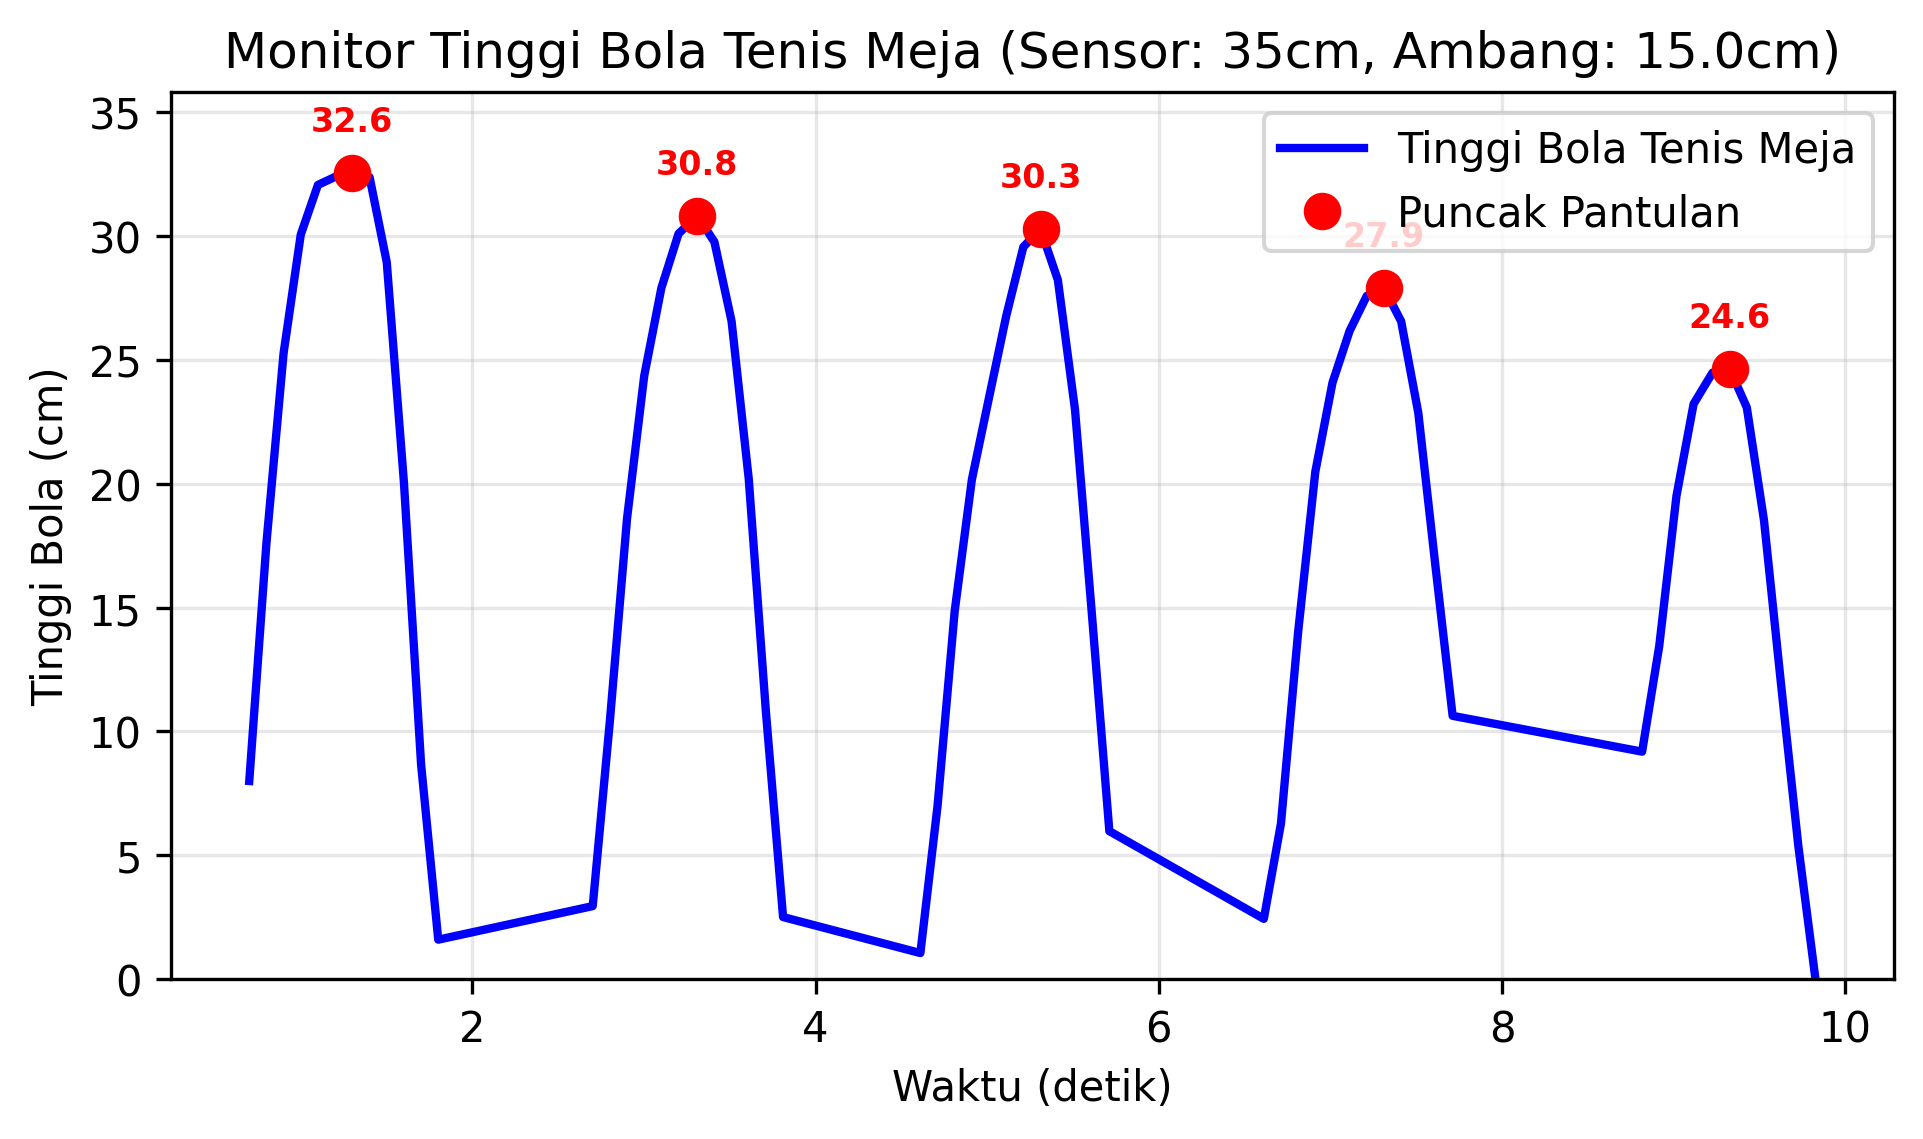
\includegraphics[width=0.5\textwidth]{chapters/DataPercobaan/Grafik_Bola_Tenis_Meja_1.png}
    \caption{Grafik Bola Tenis Meja Percobaan 1}
\end{figure}
\begin{figure}[htbp]
    \centering
    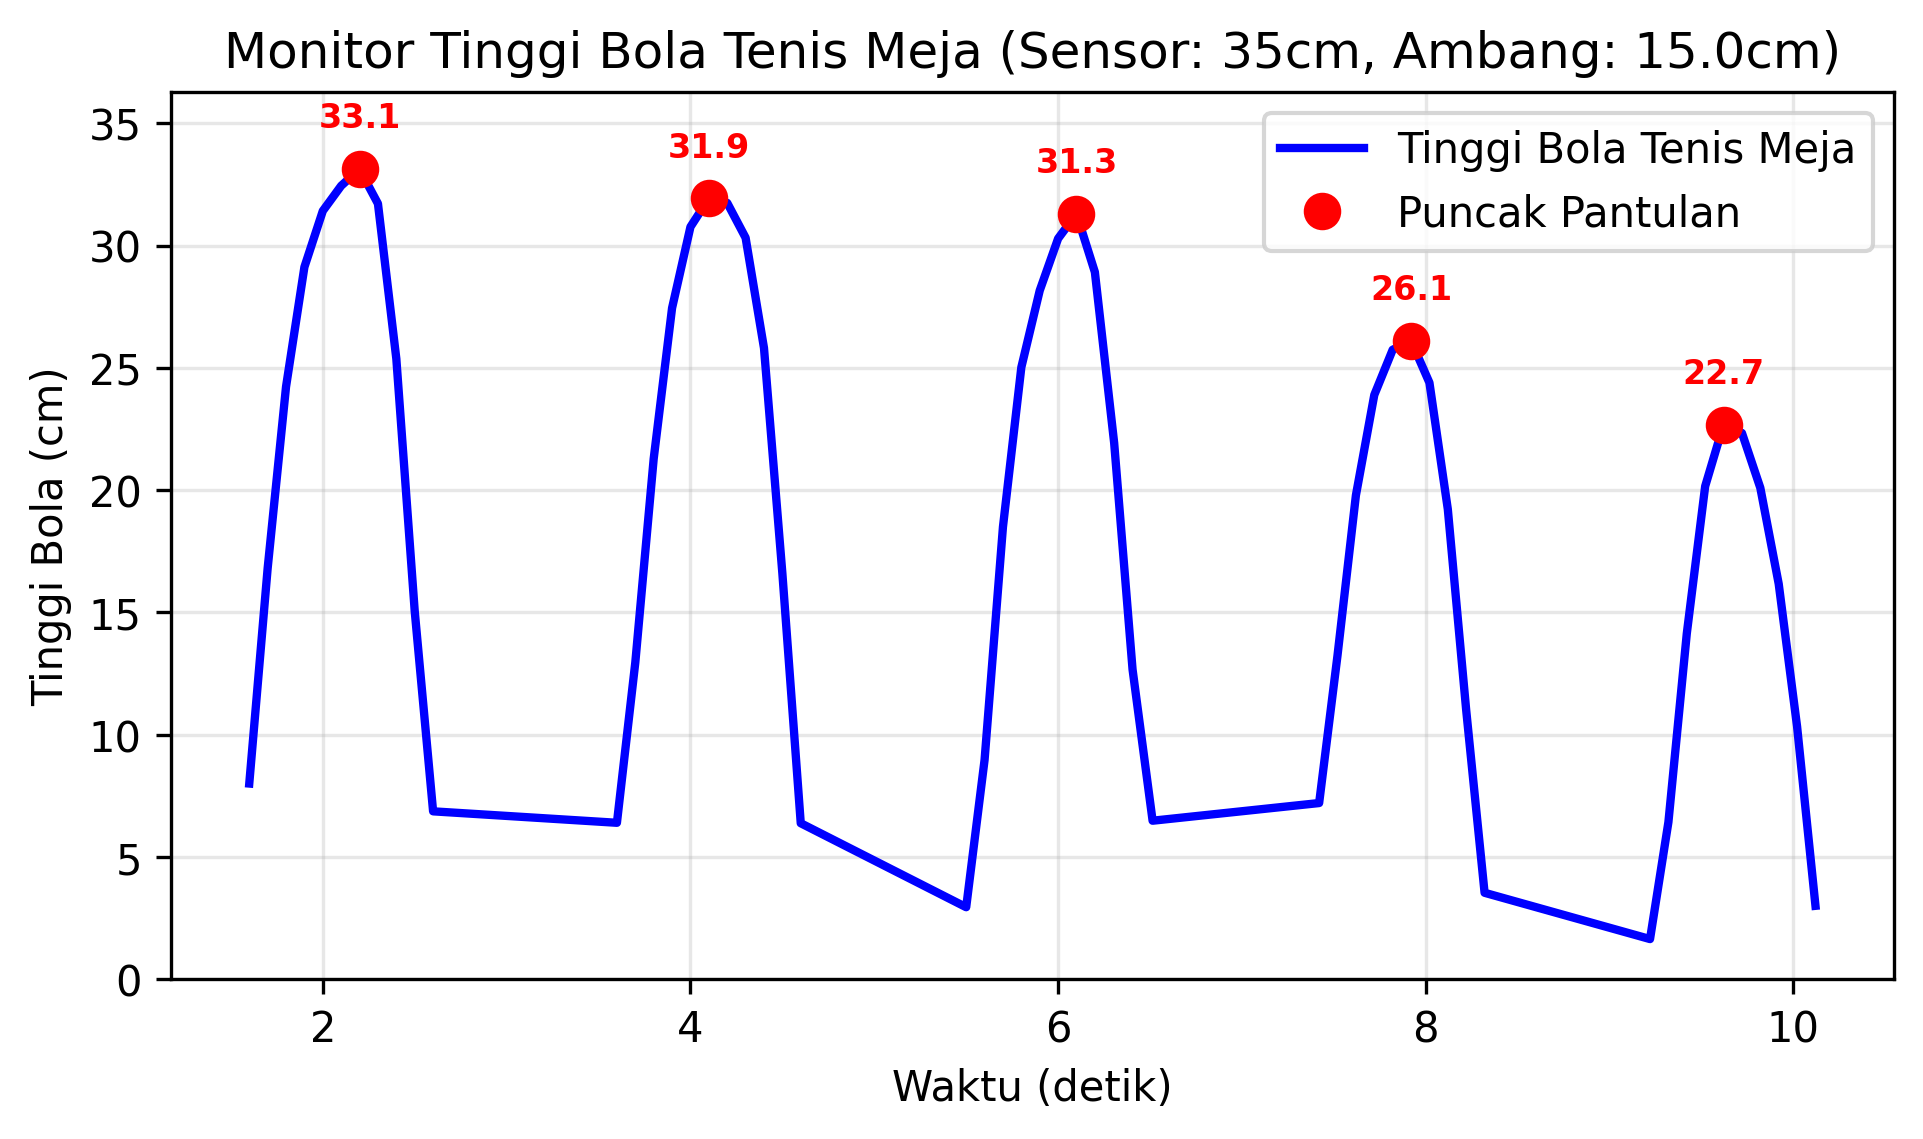
\includegraphics[width=0.5\textwidth]{chapters/DataPercobaan/Grafik_Bola_Tenis_Meja_2.png}
    \caption{Grafik Bola Tenis Meja Percobaan 2}
\end{figure}
\begin{figure}[htbp]
    \centering
    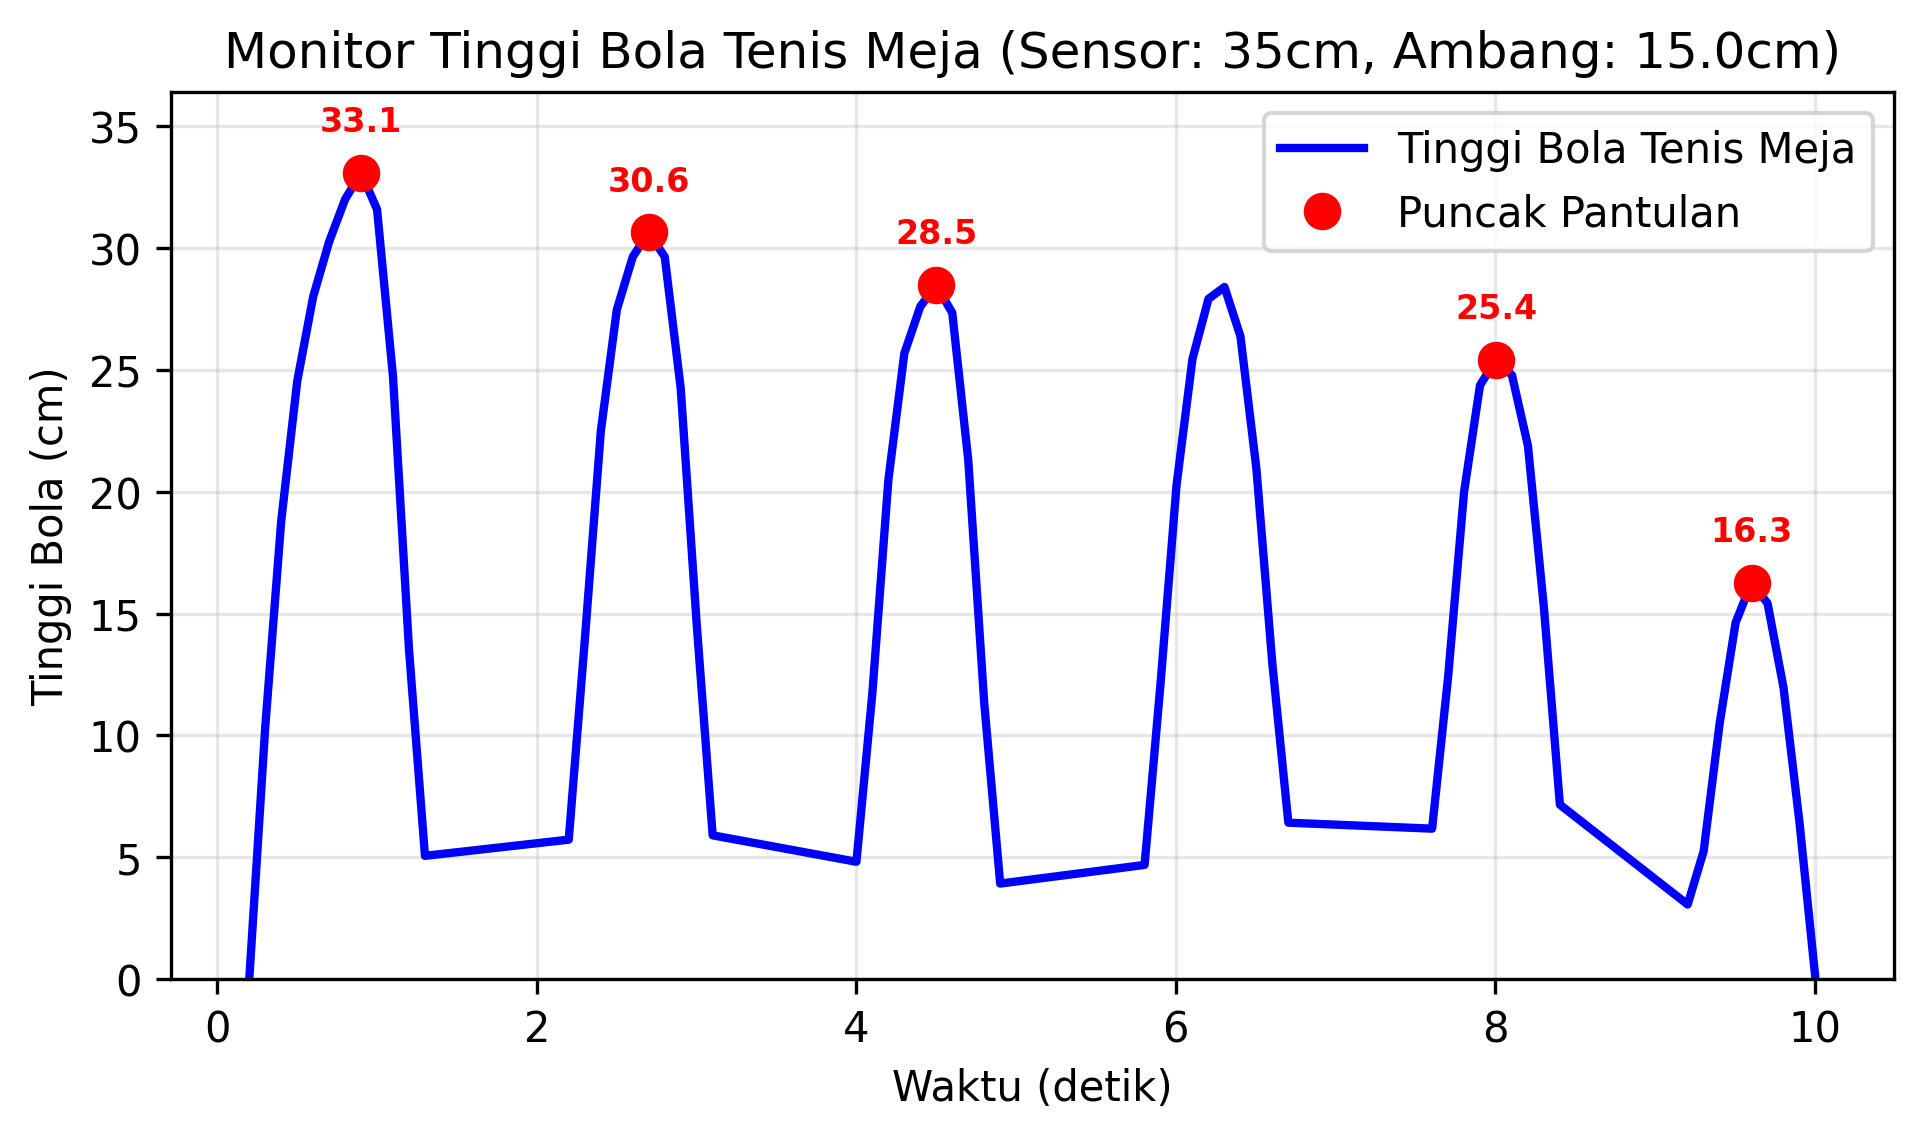
\includegraphics[width=0.5\textwidth]{chapters/DataPercobaan/Grafik_Bola_Tenis_Meja_3.png}
    \caption{Grafik Bola Tenis Meja Percobaan 3}
\end{figure}
\begin{figure}[htbp]
    \centering
    \includegraphics[width=0.5\textwidth]{chapters/DataPercobaan/Grafik_Bola_Tenis_Meja_4.png}
    \caption{Grafik Bola Tenis Meja Percobaan 4}
\end{figure}
\begin{figure}[htbp]
    \centering
    \includegraphics[width=0.5\textwidth]{chapters/DataPercobaan/Grafik_Bola_Tenis_Meja_5.png}
    \caption{Grafik Bola Tenis Meja Percobaan 5}
\end{figure}
\begin{figure}[htbp]
    \centering
    \includegraphics[width=0.5\textwidth]{chapters/DataPercobaan/Grafik_Bola_Tenis_Meja_6.png}
    \caption{Grafik Bola Tenis Meja Percobaan 6}
\end{figure}
\begin{figure}[htbp]
    \centering
    \includegraphics[width=0.5\textwidth]{chapters/DataPercobaan/Grafik_Bola_Tenis_Meja_7.png}
    \caption{Grafik Bola Tenis Meja Percobaan 7}
\end{figure}
\begin{figure}[htbp]
    \centering
    \includegraphics[width=0.5\textwidth]{chapters/DataPercobaan/Grafik_Bola_Tenis_Meja_8.png}
    \caption{Grafik Bola Tenis Meja Percobaan 8}
\end{figure}
\begin{figure}[htbp]
    \centering
    \includegraphics[width=0.5\textwidth]{chapters/DataPercobaan/Grafik_Bola_Tenis_Meja_9.png}
    \caption{Grafik Bola Tenis Meja Percobaan 9}
\end{figure}
\begin{figure}[htbp]
    \centering
    \includegraphics[width=0.5\textwidth]{chapters/DataPercobaan/Grafik_Bola_Tenis_Meja_10.png}
    \caption{Grafik Bola Tenis Meja Percobaan 10}
\end{figure}
\begin{figure}[htbp]
    \centering
    \includegraphics[width=0.5\textwidth]{chapters/DataPercobaan/Grafik_Bola_Tenis_Meja_11.png}
    \caption{Grafik Bola Tenis Meja Percobaan 11}
\end{figure}
\begin{figure}[htbp]
    \centering
    \includegraphics[width=0.5\textwidth]{chapters/DataPercobaan/Grafik_Bola_Tenis_Meja_12.png}
    \caption{Grafik Bola Tenis Meja Percobaan 12}
\end{figure}
\begin{figure}[htbp]
    \centering
    \includegraphics[width=0.5\textwidth]{chapters/DataPercobaan/Grafik_Bola_Tenis_Meja_13.png}
    \caption{Grafik Bola Tenis Meja Percobaan 13}
\end{figure}
\begin{figure}[htbp]
    \centering
    \includegraphics[width=0.5\textwidth]{chapters/DataPercobaan/Grafik_Bola_Tenis_Meja_14.png}
    \caption{Grafik Bola Tenis Meja Percobaan 14}
\end{figure}
\begin{figure}[htbp]
    \centering
    \includegraphics[width=0.5\textwidth]{chapters/DataPercobaan/Grafik_Bola_Tenis_Meja_15.png}
    \caption{Grafik Bola Tenis Meja Percobaan 15}
\end{figure}
\begin{figure}[htbp]
    \centering
    \includegraphics[width=0.5\textwidth]{chapters/DataPercobaan/Grafik_Bola_Tenis_Meja_16.png}
    \caption{Grafik Bola Tenis Meja Percobaan 16}
\end{figure}
\begin{figure}[htbp]
    \centering
    \includegraphics[width=0.5\textwidth]{chapters/DataPercobaan/Grafik_Bola_Tenis_Meja_17.png}
    \caption{Grafik Bola Tenis Meja Percobaan 17}
\end{figure}
\begin{figure}[htbp]
    \centering
    \includegraphics[width=0.5\textwidth]{chapters/DataPercobaan/Grafik_Bola_Tenis_Meja_18.png}
    \caption{Grafik Bola Tenis Meja Percobaan 18}
\end{figure}
\begin{figure}[htbp]
    \centering
    \includegraphics[width=0.5\textwidth]{chapters/DataPercobaan/Grafik_Bola_Tenis_Meja_19.png}
    \caption{Grafik Bola Tenis Meja Percobaan 19}
\end{figure}
\begin{figure}[htbp]
    \centering
    \includegraphics[width=0.5\textwidth]{chapters/DataPercobaan/Grafik_Bola_Tenis_Meja_20.png}
    \caption{Grafik Bola Tenis Meja Percobaan 20}
\end{figure}


\section{Bola Tenis Lapang}

\subsection{Tabel Percobaan}

\begin{longtable}[htbp]{|c|c|c|}
\caption{Data Bola Tenis Lapang 1} \\
\hline
Waktu (detik) & Tinggi Bola Tenis Lapang (cm) & Tinggi Sensor (cm) \\ \hline
\endfirsthead
\caption[]{Data Bola Tenis Lapang 1} \\
\hline
Waktu (detik) & Tinggi Bola Tenis Lapang (cm) & Tinggi Sensor (cm) \\ \hline
\endhead
\multicolumn{3}{r}{Continued on next page} \\
\endfoot
\endlastfoot
1.000000 & 1 & 35 \\ \hline
1.100000 & 10 & 35 \\ \hline
1.200000 & 19 & 35 \\ \hline
1.300000 & 26 & 35 \\ \hline
1.400000 & 30 & 35 \\ \hline
1.500000 & 33 & 35 \\ \hline
1.600000 & 32 & 35 \\ \hline
1.700000 & 31 & 35 \\ \hline
1.800000 & 27 & 35 \\ \hline
1.900000 & 19 & 35 \\ \hline
2.000000 & 10 & 35 \\ \hline
2.100000 & 2 & 35 \\ \hline
3.200000 & 8 & 35 \\ \hline
3.300000 & 16 & 35 \\ \hline
3.400000 & 21 & 35 \\ \hline
3.500000 & 24 & 35 \\ \hline
3.600000 & 28 & 35 \\ \hline
3.700000 & 27 & 35 \\ \hline
3.800000 & 26 & 35 \\ \hline
3.900000 & 20 & 35 \\ \hline
4.000000 & 13 & 35 \\ \hline
4.100000 & 4 & 35 \\ \hline
5.006000 & 0 & 35 \\ \hline
5.106000 & 5 & 35 \\ \hline
5.206000 & 11 & 35 \\ \hline
5.306000 & 17 & 35 \\ \hline
5.406000 & 20 & 35 \\ \hline
5.506000 & 21 & 35 \\ \hline
5.606000 & 21 & 35 \\ \hline
5.713000 & 18 & 35 \\ \hline
5.813000 & 11 & 35 \\ \hline
5.913000 & 5 & 35 \\ \hline
\end{longtable}

\begin{longtable}[htbp]{|c|c|c|}
\caption{Data Bola Tenis Lapang 2} \\
\hline
Waktu (detik) & Tinggi Bola Tenis Lapang (cm) & Tinggi Sensor (cm) \\ \hline
\endfirsthead
\caption[]{Data Bola Tenis Lapang 2} \\
\hline
Waktu (detik) & Tinggi Bola Tenis Lapang (cm) & Tinggi Sensor (cm) \\ \hline
\endhead
\multicolumn{3}{r}{Continued on next page} \\
\endfoot
\endlastfoot
0.700000 & 4 & 35 \\ \hline
0.800000 & 12 & 35 \\ \hline
0.900000 & 19 & 35 \\ \hline
1.000000 & 24 & 35 \\ \hline
1.100000 & 28 & 35 \\ \hline
1.200000 & 32 & 35 \\ \hline
1.300000 & 33 & 35 \\ \hline
1.400000 & 33 & 35 \\ \hline
1.500000 & 33 & 35 \\ \hline
1.608000 & 31 & 35 \\ \hline
1.708000 & 25 & 35 \\ \hline
1.808000 & 16 & 35 \\ \hline
1.908000 & 5 & 35 \\ \hline
2.908000 & 8 & 35 \\ \hline
3.008000 & 15 & 35 \\ \hline
3.108000 & 20 & 35 \\ \hline
3.208000 & 25 & 35 \\ \hline
3.308000 & 28 & 35 \\ \hline
3.408000 & 29 & 35 \\ \hline
3.508000 & 26 & 35 \\ \hline
3.608000 & 22 & 35 \\ \hline
3.708000 & 16 & 35 \\ \hline
3.808000 & 6 & 35 \\ \hline
4.808000 & 3 & 35 \\ \hline
4.908000 & 9 & 35 \\ \hline
5.008000 & 15 & 35 \\ \hline
5.108000 & 19 & 35 \\ \hline
5.208000 & 20 & 35 \\ \hline
5.308000 & 21 & 35 \\ \hline
5.408000 & 20 & 35 \\ \hline
5.508000 & 17 & 35 \\ \hline
5.608000 & 11 & 35 \\ \hline
5.708000 & 4 & 35 \\ \hline
\end{longtable}

\begin{longtable}[htbp]{|c|c|c|}
\caption{Data Bola Tenis Lapang 3} \\
\hline
Waktu (detik) & Tinggi Bola Tenis Lapang (cm) & Tinggi Sensor (cm) \\ \hline
\endfirsthead
\caption[]{Data Bola Tenis Lapang 3} \\
\hline
Waktu (detik) & Tinggi Bola Tenis Lapang (cm) & Tinggi Sensor (cm) \\ \hline
\endhead
\multicolumn{3}{r}{Continued on next page} \\
\endfoot
\endlastfoot
0.600000 & 10 & 35 \\ \hline
0.700000 & 19 & 35 \\ \hline
0.800000 & 27 & 35 \\ \hline
0.900000 & 31 & 35 \\ \hline
1.000000 & 33 & 35 \\ \hline
1.100000 & 32 & 35 \\ \hline
1.200000 & 19 & 35 \\ \hline
1.400000 & 29 & 35 \\ \hline
1.500000 & 19 & 35 \\ \hline
1.600000 & 7 & 35 \\ \hline
2.600000 & 4 & 35 \\ \hline
2.700000 & 11 & 35 \\ \hline
2.800000 & 18 & 35 \\ \hline
2.900000 & 22 & 35 \\ \hline
3.000000 & 26 & 35 \\ \hline
3.100000 & 26 & 35 \\ \hline
3.200000 & 23 & 35 \\ \hline
3.300000 & 18 & 35 \\ \hline
3.400000 & 9 & 35 \\ \hline
3.500000 & 0 & 35 \\ \hline
4.400000 & 0 & 35 \\ \hline
4.500000 & 6 & 35 \\ \hline
4.600000 & 13 & 35 \\ \hline
4.700000 & 16 & 35 \\ \hline
4.800000 & 17 & 35 \\ \hline
4.900000 & 16 & 35 \\ \hline
5.000000 & 12 & 35 \\ \hline
5.100000 & 5 & 35 \\ \hline
13.220000 & 0 & 35 \\ \hline
13.320000 & 0 & 35 \\ \hline
13.420000 & 2 & 35 \\ \hline
13.520000 & 1 & 35 \\ \hline
13.620000 & 0 & 35 \\ \hline
13.820000 & 0 & 35 \\ \hline
13.920000 & 0 & 35 \\ \hline
14.520000 & 0 & 35 \\ \hline
14.620000 & 0 & 35 \\ \hline
\end{longtable}

\begin{longtable}[htbp]{|c|c|c|}
\caption{Data Bola Tenis Lapang 4} \\
\hline
Waktu (detik) & Tinggi Bola Tenis Lapang (cm) & Tinggi Sensor (cm) \\ \hline
\endfirsthead
\caption[]{Data Bola Tenis Lapang 4} \\
\hline
Waktu (detik) & Tinggi Bola Tenis Lapang (cm) & Tinggi Sensor (cm) \\ \hline
\endhead
\multicolumn{3}{r}{Continued on next page} \\
\endfoot
\endlastfoot
0.100000 & 1 & 35 \\ \hline
0.200000 & 10 & 35 \\ \hline
0.300000 & 19 & 35 \\ \hline
0.400000 & 27 & 35 \\ \hline
0.500000 & 32 & 35 \\ \hline
0.600000 & 33 & 35 \\ \hline
0.700000 & 33 & 35 \\ \hline
0.800000 & 30 & 35 \\ \hline
0.900000 & 21 & 35 \\ \hline
1.000000 & 10 & 35 \\ \hline
1.915000 & 2 & 35 \\ \hline
2.015000 & 8 & 35 \\ \hline
2.115000 & 21 & 35 \\ \hline
2.215000 & 26 & 35 \\ \hline
2.315000 & 27 & 35 \\ \hline
2.415000 & 25 & 35 \\ \hline
2.515000 & 21 & 35 \\ \hline
2.615000 & 14 & 35 \\ \hline
2.715000 & 4 & 35 \\ \hline
3.717000 & 8 & 35 \\ \hline
3.817000 & 17 & 35 \\ \hline
3.917000 & 21 & 35 \\ \hline
4.017000 & 21 & 35 \\ \hline
4.117000 & 19 & 35 \\ \hline
4.217000 & 14 & 35 \\ \hline
4.317000 & 5 & 35 \\ \hline
\end{longtable}

\begin{longtable}[htbp]{|c|c|c|}
\caption{Data Bola Tenis Lapang 5} \\
\hline
Waktu (detik) & Tinggi Bola Tenis Lapang (cm) & Tinggi Sensor (cm) \\ \hline
\endfirsthead
\caption[]{Data Bola Tenis Lapang 5} \\
\hline
Waktu (detik) & Tinggi Bola Tenis Lapang (cm) & Tinggi Sensor (cm) \\ \hline
\endhead
\multicolumn{3}{r}{Continued on next page} \\
\endfoot
\endlastfoot
0.707000 & 6 & 35 \\ \hline
0.807000 & 14 & 35 \\ \hline
0.907000 & 23 & 35 \\ \hline
1.007000 & 30 & 35 \\ \hline
1.107000 & 32 & 35 \\ \hline
1.207000 & 29 & 35 \\ \hline
1.407000 & 32 & 35 \\ \hline
1.507000 & 32 & 35 \\ \hline
1.607000 & 24 & 35 \\ \hline
1.707000 & 13 & 35 \\ \hline
2.607000 & 3 & 35 \\ \hline
2.707000 & 12 & 35 \\ \hline
2.807000 & 20 & 35 \\ \hline
2.907000 & 25 & 35 \\ \hline
3.007000 & 28 & 35 \\ \hline
3.107000 & 28 & 35 \\ \hline
3.207000 & 27 & 35 \\ \hline
3.307000 & 22 & 35 \\ \hline
3.407000 & 15 & 35 \\ \hline
3.507000 & 5 & 35 \\ \hline
4.407000 & 1 & 35 \\ \hline
4.507000 & 8 & 35 \\ \hline
4.607000 & 14 & 35 \\ \hline
4.707000 & 19 & 35 \\ \hline
4.807000 & 22 & 35 \\ \hline
4.907000 & 21 & 35 \\ \hline
5.011000 & 19 & 35 \\ \hline
5.111000 & 13 & 35 \\ \hline
5.211000 & 4 & 35 \\ \hline
\end{longtable}

\begin{longtable}[htbp]{|c|c|c|}
\caption{Data Bola Tenis Lapang 6} \\
\hline
Waktu (detik) & Tinggi Bola Tenis Lapang (cm) & Tinggi Sensor (cm) \\ \hline
\endfirsthead
\caption[]{Data Bola Tenis Lapang 6} \\
\hline
Waktu (detik) & Tinggi Bola Tenis Lapang (cm) & Tinggi Sensor (cm) \\ \hline
\endhead
\multicolumn{3}{r}{Continued on next page} \\
\endfoot
\endlastfoot
0.774657 & 2 & 35 \\ \hline
1.000000 & 1 & 35 \\ \hline
1.100000 & 11 & 35 \\ \hline
1.200000 & 20 & 35 \\ \hline
1.300000 & 26 & 35 \\ \hline
1.400000 & 31 & 35 \\ \hline
1.500000 & 32 & 35 \\ \hline
1.600000 & 32 & 35 \\ \hline
1.700000 & 28 & 35 \\ \hline
1.800000 & 20 & 35 \\ \hline
1.900000 & 11 & 35 \\ \hline
2.000000 & 0 & 35 \\ \hline
2.800000 & 0 & 35 \\ \hline
2.900000 & 8 & 35 \\ \hline
3.000000 & 16 & 35 \\ \hline
3.100000 & 22 & 35 \\ \hline
3.200000 & 26 & 35 \\ \hline
3.300000 & 29 & 35 \\ \hline
3.400000 & 27 & 35 \\ \hline
3.500000 & 22 & 35 \\ \hline
3.600000 & 16 & 35 \\ \hline
3.700000 & 6 & 35 \\ \hline
4.600000 & 5 & 35 \\ \hline
4.700000 & 13 & 35 \\ \hline
4.800000 & 18 & 35 \\ \hline
4.900000 & 22 & 35 \\ \hline
5.000000 & 25 & 35 \\ \hline
5.100000 & 23 & 35 \\ \hline
5.200000 & 19 & 35 \\ \hline
5.300000 & 13 & 35 \\ \hline
5.400000 & 2 & 35 \\ \hline
\end{longtable}

\begin{longtable}[htbp]{|c|c|c|}
\caption{Data Bola Tenis Lapang 7} \\
\hline
Waktu (detik) & Tinggi Bola Tenis Lapang (cm) & Tinggi Sensor (cm) \\ \hline
\endfirsthead
\caption[]{Data Bola Tenis Lapang 7} \\
\hline
Waktu (detik) & Tinggi Bola Tenis Lapang (cm) & Tinggi Sensor (cm) \\ \hline
\endhead
\multicolumn{3}{r}{Continued on next page} \\
\endfoot
\endlastfoot
0.700000 & 16 & 35 \\ \hline
0.800000 & 24 & 35 \\ \hline
0.900000 & 30 & 35 \\ \hline
1.000000 & 33 & 35 \\ \hline
1.100000 & 32 & 35 \\ \hline
1.200000 & 32 & 35 \\ \hline
1.300000 & 32 & 35 \\ \hline
1.400000 & 28 & 35 \\ \hline
1.500000 & 19 & 35 \\ \hline
1.600000 & 10 & 35 \\ \hline
2.500000 & 5 & 35 \\ \hline
2.600000 & 12 & 35 \\ \hline
2.705000 & 19 & 35 \\ \hline
2.805000 & 23 & 35 \\ \hline
2.905000 & 26 & 35 \\ \hline
3.005000 & 25 & 35 \\ \hline
3.105000 & 22 & 35 \\ \hline
3.205000 & 19 & 35 \\ \hline
3.305000 & 13 & 35 \\ \hline
3.405000 & 3 & 35 \\ \hline
4.305000 & 0 & 35 \\ \hline
4.405000 & 6 & 35 \\ \hline
4.505000 & 11 & 35 \\ \hline
4.605000 & 15 & 35 \\ \hline
4.705000 & 16 & 35 \\ \hline
4.805000 & 14 & 35 \\ \hline
4.909000 & 12 & 35 \\ \hline
5.009000 & 6 & 35 \\ \hline
5.109000 & 0 & 35 \\ \hline
\end{longtable}

\begin{longtable}[htbp]{|c|c|c|}
\caption{Data Bola Tenis Lapang 8} \\
\hline
Waktu (detik) & Tinggi Bola Tenis Lapang (cm) & Tinggi Sensor (cm) \\ \hline
\endfirsthead
\caption[]{Data Bola Tenis Lapang 8} \\
\hline
Waktu (detik) & Tinggi Bola Tenis Lapang (cm) & Tinggi Sensor (cm) \\ \hline
\endhead
\multicolumn{3}{r}{Continued on next page} \\
\endfoot
\endlastfoot
0.507000 & 6 & 35 \\ \hline
0.607000 & 15 & 35 \\ \hline
0.707000 & 23 & 35 \\ \hline
0.807000 & 27 & 35 \\ \hline
0.907000 & 30 & 35 \\ \hline
1.007000 & 30 & 35 \\ \hline
1.107000 & 25 & 35 \\ \hline
1.207000 & 17 & 35 \\ \hline
1.307000 & 8 & 35 \\ \hline
2.307000 & 3 & 35 \\ \hline
2.407000 & 10 & 35 \\ \hline
2.507000 & 19 & 35 \\ \hline
2.607000 & 24 & 35 \\ \hline
2.710000 & 27 & 35 \\ \hline
2.810000 & 27 & 35 \\ \hline
2.910000 & 25 & 35 \\ \hline
3.010000 & 19 & 35 \\ \hline
3.110000 & 11 & 35 \\ \hline
3.210000 & 2 & 35 \\ \hline
4.018000 & 6 & 35 \\ \hline
4.118000 & 12 & 35 \\ \hline
4.218000 & 16 & 35 \\ \hline
4.319000 & 16 & 35 \\ \hline
4.419000 & 12 & 35 \\ \hline
4.519000 & 4 & 35 \\ \hline
\end{longtable}

\begin{longtable}[htbp]{|c|c|c|}
\caption{Data Bola Tenis Lapang 9} \\
\hline
Waktu (detik) & Tinggi Bola Tenis Lapang (cm) & Tinggi Sensor (cm) \\ \hline
\endfirsthead
\caption[]{Data Bola Tenis Lapang 9} \\
\hline
Waktu (detik) & Tinggi Bola Tenis Lapang (cm) & Tinggi Sensor (cm) \\ \hline
\endhead
\multicolumn{3}{r}{Continued on next page} \\
\endfoot
\endlastfoot
0.400000 & 0 & 35 \\ \hline
0.500000 & 10 & 35 \\ \hline
0.600000 & 18 & 35 \\ \hline
0.700000 & 24 & 35 \\ \hline
0.800000 & 29 & 35 \\ \hline
0.900000 & 29 & 35 \\ \hline
1.000000 & 26 & 35 \\ \hline
1.109000 & 22 & 35 \\ \hline
1.209000 & 14 & 35 \\ \hline
1.313000 & 6 & 35 \\ \hline
2.417000 & 4 & 35 \\ \hline
2.517000 & 12 & 35 \\ \hline
2.617000 & 19 & 35 \\ \hline
2.717000 & 25 & 35 \\ \hline
2.817000 & 26 & 35 \\ \hline
2.917000 & 24 & 35 \\ \hline
3.017000 & 18 & 35 \\ \hline
3.118000 & 7 & 35 \\ \hline
3.218000 & 1 & 35 \\ \hline
4.228000 & 4 & 35 \\ \hline
4.328000 & 10 & 35 \\ \hline
4.428000 & 15 & 35 \\ \hline
4.528000 & 17 & 35 \\ \hline
4.628000 & 19 & 35 \\ \hline
4.728000 & 17 & 35 \\ \hline
4.828000 & 13 & 35 \\ \hline
4.928000 & 6 & 35 \\ \hline
\end{longtable}

\begin{longtable}[htbp]{|c|c|c|}
\caption{Data Bola Tenis Lapang 10} \\
\hline
Waktu (detik) & Tinggi Bola Tenis Lapang (cm) & Tinggi Sensor (cm) \\ \hline
\endfirsthead
\caption[]{Data Bola Tenis Lapang 10} \\
\hline
Waktu (detik) & Tinggi Bola Tenis Lapang (cm) & Tinggi Sensor (cm) \\ \hline
\endhead
\multicolumn{3}{r}{Continued on next page} \\
\endfoot
\endlastfoot
2.707000 & 7 & 35 \\ \hline
2.807000 & 18 & 35 \\ \hline
2.907000 & 25 & 35 \\ \hline
3.007000 & 31 & 35 \\ \hline
3.107000 & 33 & 35 \\ \hline
3.207000 & 33 & 35 \\ \hline
3.307000 & 28 & 35 \\ \hline
3.408000 & 22 & 35 \\ \hline
3.508000 & 12 & 35 \\ \hline
3.608000 & 2 & 35 \\ \hline
4.415000 & 2 & 35 \\ \hline
4.515000 & 11 & 35 \\ \hline
4.622000 & 20 & 35 \\ \hline
4.722000 & 25 & 35 \\ \hline
4.822000 & 27 & 35 \\ \hline
4.922000 & 27 & 35 \\ \hline
5.022000 & 23 & 35 \\ \hline
5.122000 & 12 & 35 \\ \hline
5.222000 & 8 & 35 \\ \hline
6.122000 & 5 & 35 \\ \hline
6.222000 & 13 & 35 \\ \hline
6.322000 & 18 & 35 \\ \hline
6.422000 & 20 & 35 \\ \hline
6.522000 & 20 & 35 \\ \hline
6.622000 & 16 & 35 \\ \hline
6.722000 & 7 & 35 \\ \hline
6.822000 & 1 & 35 \\ \hline
\end{longtable}

\begin{longtable}[htbp]{|c|c|c|}
\caption{Data Bola Tenis Lapang 11} \\
\hline
Waktu (detik) & Tinggi Bola Tenis Lapang (cm) & Tinggi Sensor (cm) \\ \hline
\endfirsthead
\caption[]{Data Bola Tenis Lapang 11} \\
\hline
Waktu (detik) & Tinggi Bola Tenis Lapang (cm) & Tinggi Sensor (cm) \\ \hline
\endhead
\multicolumn{3}{r}{Continued on next page} \\
\endfoot
\endlastfoot
1.101000 & 3 & 35 \\ \hline
1.201000 & 12 & 35 \\ \hline
1.301000 & 20 & 35 \\ \hline
1.401000 & 28 & 35 \\ \hline
1.501000 & 31 & 35 \\ \hline
1.601000 & 32 & 35 \\ \hline
1.701000 & 33 & 35 \\ \hline
1.801000 & 29 & 35 \\ \hline
1.901000 & 22 & 35 \\ \hline
2.001000 & 13 & 35 \\ \hline
2.101000 & 5 & 35 \\ \hline
3.005000 & 6 & 35 \\ \hline
3.105000 & 13 & 35 \\ \hline
3.205000 & 20 & 35 \\ \hline
3.305000 & 25 & 35 \\ \hline
3.405000 & 28 & 35 \\ \hline
3.505000 & 28 & 35 \\ \hline
3.605000 & 24 & 35 \\ \hline
3.705000 & 19 & 35 \\ \hline
3.805000 & 9 & 35 \\ \hline
3.905000 & 0 & 35 \\ \hline
4.805000 & 0 & 35 \\ \hline
4.905000 & 6 & 35 \\ \hline
5.005000 & 13 & 35 \\ \hline
5.105000 & 19 & 35 \\ \hline
5.205000 & 20 & 35 \\ \hline
5.305000 & 19 & 35 \\ \hline
5.405000 & 17 & 35 \\ \hline
5.505000 & 11 & 35 \\ \hline
5.605000 & 4 & 35 \\ \hline
\end{longtable}

\begin{longtable}[htbp]{|c|c|c|}
\caption{Data Bola Tenis Lapang 12} \\
\hline
Waktu (detik) & Tinggi Bola Tenis Lapang (cm) & Tinggi Sensor (cm) \\ \hline
\endfirsthead
\caption[]{Data Bola Tenis Lapang 12} \\
\hline
Waktu (detik) & Tinggi Bola Tenis Lapang (cm) & Tinggi Sensor (cm) \\ \hline
\endhead
\multicolumn{3}{r}{Continued on next page} \\
\endfoot
\endlastfoot
0.500000 & 8 & 35 \\ \hline
0.600000 & 18 & 35 \\ \hline
0.700000 & 26 & 35 \\ \hline
0.800000 & 30 & 35 \\ \hline
0.900000 & 33 & 35 \\ \hline
1.000000 & 33 & 35 \\ \hline
1.100000 & 33 & 35 \\ \hline
1.200000 & 30 & 35 \\ \hline
1.300000 & 21 & 35 \\ \hline
1.400000 & 7 & 35 \\ \hline
1.500000 & 2 & 35 \\ \hline
2.311000 & 6 & 35 \\ \hline
2.411000 & 14 & 35 \\ \hline
2.511000 & 22 & 35 \\ \hline
2.611000 & 26 & 35 \\ \hline
2.711000 & 28 & 35 \\ \hline
2.811000 & 28 & 35 \\ \hline
2.911000 & 26 & 35 \\ \hline
3.011000 & 21 & 35 \\ \hline
3.111000 & 13 & 35 \\ \hline
3.211000 & 5 & 35 \\ \hline
4.112000 & 4 & 35 \\ \hline
4.212000 & 10 & 35 \\ \hline
4.312000 & 16 & 35 \\ \hline
4.412000 & 20 & 35 \\ \hline
4.512000 & 21 & 35 \\ \hline
4.621000 & 22 & 35 \\ \hline
4.721000 & 19 & 35 \\ \hline
4.821000 & 13 & 35 \\ \hline
4.921000 & 10 & 35 \\ \hline
5.021000 & 2 & 35 \\ \hline
\end{longtable}

\begin{longtable}[htbp]{|c|c|c|}
\caption{Data Bola Tenis Lapang 13} \\
\hline
Waktu (detik) & Tinggi Bola Tenis Lapang (cm) & Tinggi Sensor (cm) \\ \hline
\endfirsthead
\caption[]{Data Bola Tenis Lapang 13} \\
\hline
Waktu (detik) & Tinggi Bola Tenis Lapang (cm) & Tinggi Sensor (cm) \\ \hline
\endhead
\multicolumn{3}{r}{Continued on next page} \\
\endfoot
\endlastfoot
0.101000 & 0 & 35 \\ \hline
0.201000 & 11 & 35 \\ \hline
0.301000 & 20 & 35 \\ \hline
0.401000 & 26 & 35 \\ \hline
0.502000 & 31 & 35 \\ \hline
0.602000 & 32 & 35 \\ \hline
0.710000 & 32 & 35 \\ \hline
0.810000 & 28 & 35 \\ \hline
0.910000 & 22 & 35 \\ \hline
1.010000 & 12 & 35 \\ \hline
1.110000 & 2 & 35 \\ \hline
1.910000 & 1 & 35 \\ \hline
2.010000 & 12 & 35 \\ \hline
2.110000 & 19 & 35 \\ \hline
2.210000 & 25 & 35 \\ \hline
2.310000 & 28 & 35 \\ \hline
2.410000 & 30 & 35 \\ \hline
2.511000 & 27 & 35 \\ \hline
2.611000 & 24 & 35 \\ \hline
2.711000 & 15 & 35 \\ \hline
2.811000 & 6 & 35 \\ \hline
3.611000 & 2 & 35 \\ \hline
3.711000 & 10 & 35 \\ \hline
3.811000 & 18 & 35 \\ \hline
3.911000 & 20 & 35 \\ \hline
4.011000 & 20 & 35 \\ \hline
4.115000 & 15 & 35 \\ \hline
4.215000 & 6 & 35 \\ \hline
\end{longtable}

\begin{longtable}[htbp]{|c|c|c|}
\caption{Data Bola Tenis Lapang 14} \\
\hline
Waktu (detik) & Tinggi Bola Tenis Lapang (cm) & Tinggi Sensor (cm) \\ \hline
\endfirsthead
\caption[]{Data Bola Tenis Lapang 14} \\
\hline
Waktu (detik) & Tinggi Bola Tenis Lapang (cm) & Tinggi Sensor (cm) \\ \hline
\endhead
\multicolumn{3}{r}{Continued on next page} \\
\endfoot
\endlastfoot
0.600000 & 3 & 35 \\ \hline
0.700000 & 10 & 35 \\ \hline
0.800000 & 19 & 35 \\ \hline
0.900000 & 25 & 35 \\ \hline
1.000000 & 29 & 35 \\ \hline
1.100000 & 30 & 35 \\ \hline
1.200000 & 31 & 35 \\ \hline
1.300000 & 31 & 35 \\ \hline
1.400000 & 28 & 35 \\ \hline
1.500000 & 24 & 35 \\ \hline
1.600000 & 16 & 35 \\ \hline
1.700000 & 7 & 35 \\ \hline
2.713000 & 6 & 35 \\ \hline
2.813000 & 14 & 35 \\ \hline
2.913000 & 17 & 35 \\ \hline
3.013000 & 26 & 35 \\ \hline
3.113000 & 28 & 35 \\ \hline
3.213000 & 28 & 35 \\ \hline
3.313000 & 24 & 35 \\ \hline
3.413000 & 19 & 35 \\ \hline
3.513000 & 12 & 35 \\ \hline
3.613000 & 4 & 35 \\ \hline
4.513000 & 1 & 35 \\ \hline
4.613000 & 8 & 35 \\ \hline
4.713000 & 15 & 35 \\ \hline
4.813000 & 24 & 35 \\ \hline
4.913000 & 26 & 35 \\ \hline
5.013000 & 27 & 35 \\ \hline
5.118000 & 24 & 35 \\ \hline
5.218000 & 19 & 35 \\ \hline
5.319000 & 11 & 35 \\ \hline
5.419000 & 3 & 35 \\ \hline
6.419000 & 0 & 35 \\ \hline
\end{longtable}

\begin{longtable}[htbp]{|c|c|c|}
\caption{Data Bola Tenis Lapang 15} \\
\hline
Waktu (detik) & Tinggi Bola Tenis Lapang (cm) & Tinggi Sensor (cm) \\ \hline
\endfirsthead
\caption[]{Data Bola Tenis Lapang 15} \\
\hline
Waktu (detik) & Tinggi Bola Tenis Lapang (cm) & Tinggi Sensor (cm) \\ \hline
\endhead
\multicolumn{3}{r}{Continued on next page} \\
\endfoot
\endlastfoot
0.200000 & 6 & 35 \\ \hline
0.300000 & 16 & 35 \\ \hline
0.400000 & 25 & 35 \\ \hline
0.500000 & 30 & 35 \\ \hline
0.600000 & 32 & 35 \\ \hline
0.700000 & 31 & 35 \\ \hline
0.800000 & 32 & 35 \\ \hline
0.900000 & 27 & 35 \\ \hline
1.000000 & 19 & 35 \\ \hline
1.100000 & 11 & 35 \\ \hline
1.200000 & 2 & 35 \\ \hline
2.200000 & 3 & 35 \\ \hline
2.300000 & 9 & 35 \\ \hline
2.400000 & 17 & 35 \\ \hline
2.501000 & 25 & 35 \\ \hline
2.601000 & 29 & 35 \\ \hline
2.701000 & 31 & 35 \\ \hline
2.801000 & 29 & 35 \\ \hline
2.901000 & 24 & 35 \\ \hline
3.001000 & 17 & 35 \\ \hline
3.101000 & 8 & 35 \\ \hline
4.010000 & 0 & 35 \\ \hline
4.110000 & 7 & 35 \\ \hline
4.210000 & 14 & 35 \\ \hline
4.310000 & 19 & 35 \\ \hline
4.410000 & 20 & 35 \\ \hline
4.510000 & 19 & 35 \\ \hline
4.610000 & 15 & 35 \\ \hline
4.711000 & 6 & 35 \\ \hline
\end{longtable}

\begin{longtable}[htbp]{|c|c|c|}
\caption{Data Bola Tenis Lapang 16} \\
\hline
Waktu (detik) & Tinggi Bola Tenis Lapang (cm) & Tinggi Sensor (cm) \\ \hline
\endfirsthead
\caption[]{Data Bola Tenis Lapang 16} \\
\hline
Waktu (detik) & Tinggi Bola Tenis Lapang (cm) & Tinggi Sensor (cm) \\ \hline
\endhead
\multicolumn{3}{r}{Continued on next page} \\
\endfoot
\endlastfoot
0.200000 & 5 & 35 \\ \hline
0.300000 & 14 & 35 \\ \hline
0.400000 & 22 & 35 \\ \hline
0.500000 & 30 & 35 \\ \hline
0.600000 & 32 & 35 \\ \hline
0.700000 & 33 & 35 \\ \hline
0.800000 & 32 & 35 \\ \hline
0.900000 & 26 & 35 \\ \hline
1.000000 & 16 & 35 \\ \hline
1.100000 & 3 & 35 \\ \hline
2.002000 & 4 & 35 \\ \hline
2.102000 & 13 & 35 \\ \hline
2.202000 & 20 & 35 \\ \hline
2.302000 & 28 & 35 \\ \hline
2.402000 & 30 & 35 \\ \hline
2.502000 & 30 & 35 \\ \hline
2.602000 & 26 & 35 \\ \hline
2.702000 & 19 & 35 \\ \hline
2.808000 & 12 & 35 \\ \hline
2.908000 & 3 & 35 \\ \hline
3.708000 & 0 & 35 \\ \hline
3.808000 & 8 & 35 \\ \hline
3.908000 & 16 & 35 \\ \hline
4.008000 & 20 & 35 \\ \hline
4.108000 & 25 & 35 \\ \hline
4.211000 & 24 & 35 \\ \hline
4.311000 & 24 & 35 \\ \hline
4.411000 & 19 & 35 \\ \hline
4.511000 & 13 & 35 \\ \hline
4.611000 & 5 & 35 \\ \hline
\end{longtable}

\begin{longtable}[htbp]{|c|c|c|}
\caption{Data Bola Tenis Lapang 17} \\
\hline
Waktu (detik) & Tinggi Bola Tenis Lapang (cm) & Tinggi Sensor (cm) \\ \hline
\endfirsthead
\caption[]{Data Bola Tenis Lapang 17} \\
\hline
Waktu (detik) & Tinggi Bola Tenis Lapang (cm) & Tinggi Sensor (cm) \\ \hline
\endhead
\multicolumn{3}{r}{Continued on next page} \\
\endfoot
\endlastfoot
0.400000 & 5 & 35 \\ \hline
0.500000 & 16 & 35 \\ \hline
0.600000 & 25 & 35 \\ \hline
0.700000 & 29 & 35 \\ \hline
0.800000 & 32 & 35 \\ \hline
0.900000 & 33 & 35 \\ \hline
1.000000 & 33 & 35 \\ \hline
1.100000 & 31 & 35 \\ \hline
1.207000 & 24 & 35 \\ \hline
1.307000 & 16 & 35 \\ \hline
1.413000 & 6 & 35 \\ \hline
2.313000 & 2 & 35 \\ \hline
2.413000 & 9 & 35 \\ \hline
2.513000 & 17 & 35 \\ \hline
2.613000 & 23 & 35 \\ \hline
2.715000 & 27 & 35 \\ \hline
2.815000 & 29 & 35 \\ \hline
2.915000 & 29 & 35 \\ \hline
3.020000 & 26 & 35 \\ \hline
3.120000 & 19 & 35 \\ \hline
3.220000 & 10 & 35 \\ \hline
3.320000 & 2 & 35 \\ \hline
4.120000 & 2 & 35 \\ \hline
4.220000 & 10 & 35 \\ \hline
4.320000 & 18 & 35 \\ \hline
4.420000 & 22 & 35 \\ \hline
4.520000 & 25 & 35 \\ \hline
4.620000 & 24 & 35 \\ \hline
4.720000 & 20 & 35 \\ \hline
4.820000 & 13 & 35 \\ \hline
4.920000 & 4 & 35 \\ \hline
\end{longtable}

\begin{longtable}[htbp]{|c|c|c|}
\caption{Data Bola Tenis Lapang 18} \\
\hline
Waktu (detik) & Tinggi Bola Tenis Lapang (cm) & Tinggi Sensor (cm) \\ \hline
\endfirsthead
\caption[]{Data Bola Tenis Lapang 18} \\
\hline
Waktu (detik) & Tinggi Bola Tenis Lapang (cm) & Tinggi Sensor (cm) \\ \hline
\endhead
\multicolumn{3}{r}{Continued on next page} \\
\endfoot
\endlastfoot
0.500000 & 2 & 35 \\ \hline
0.600000 & 12 & 35 \\ \hline
0.700000 & 21 & 35 \\ \hline
0.809000 & 28 & 35 \\ \hline
0.909000 & 32 & 35 \\ \hline
1.009000 & 32 & 35 \\ \hline
1.109000 & 28 & 35 \\ \hline
1.209000 & 20 & 35 \\ \hline
1.309000 & 11 & 35 \\ \hline
2.310000 & 6 & 35 \\ \hline
2.410000 & 14 & 35 \\ \hline
2.510000 & 19 & 35 \\ \hline
2.610000 & 24 & 35 \\ \hline
2.710000 & 28 & 35 \\ \hline
2.810000 & 29 & 35 \\ \hline
2.910000 & 26 & 35 \\ \hline
3.010000 & 21 & 35 \\ \hline
3.110000 & 14 & 35 \\ \hline
3.210000 & 5 & 35 \\ \hline
4.120000 & 3 & 35 \\ \hline
4.220000 & 9 & 35 \\ \hline
4.320000 & 15 & 35 \\ \hline
4.420000 & 19 & 35 \\ \hline
4.526000 & 22 & 35 \\ \hline
4.626000 & 21 & 35 \\ \hline
4.726000 & 19 & 35 \\ \hline
4.826000 & 13 & 35 \\ \hline
4.926000 & 5 & 35 \\ \hline
\end{longtable}

\begin{longtable}[htbp]{|c|c|c|}
\caption{Data Bola Tenis Lapang 19} \\
\hline
Waktu (detik) & Tinggi Bola Tenis Lapang (cm) & Tinggi Sensor (cm) \\ \hline
\endfirsthead
\caption[]{Data Bola Tenis Lapang 19} \\
\hline
Waktu (detik) & Tinggi Bola Tenis Lapang (cm) & Tinggi Sensor (cm) \\ \hline
\endhead
\multicolumn{3}{r}{Continued on next page} \\
\endfoot
\endlastfoot
0.330000 & 6 & 35 \\ \hline
0.430000 & 17 & 35 \\ \hline
0.530000 & 23 & 35 \\ \hline
0.630000 & 29 & 35 \\ \hline
0.730000 & 32 & 35 \\ \hline
0.830000 & 32 & 35 \\ \hline
0.930000 & 31 & 35 \\ \hline
1.030000 & 26 & 35 \\ \hline
1.139000 & 17 & 35 \\ \hline
1.239000 & 8 & 35 \\ \hline
2.139000 & 0 & 35 \\ \hline
2.239000 & 9 & 35 \\ \hline
2.339000 & 18 & 35 \\ \hline
2.439000 & 23 & 35 \\ \hline
2.539000 & 26 & 35 \\ \hline
2.639000 & 27 & 35 \\ \hline
2.739000 & 22 & 35 \\ \hline
2.839000 & 16 & 35 \\ \hline
2.939000 & 6 & 35 \\ \hline
3.939000 & 6 & 35 \\ \hline
4.039000 & 13 & 35 \\ \hline
4.139000 & 16 & 35 \\ \hline
4.239000 & 17 & 35 \\ \hline
4.339000 & 15 & 35 \\ \hline
4.439000 & 10 & 35 \\ \hline
4.539000 & 5 & 35 \\ \hline
\end{longtable}

\begin{longtable}[htbp]{|c|c|c|}
\caption{Data Bola Tenis Lapang 20} \\
\hline
Waktu (detik) & Tinggi Bola Tenis Lapang (cm) & Tinggi Sensor (cm) \\ \hline
\endfirsthead
\caption[]{Data Bola Tenis Lapang 20} \\
\hline
Waktu (detik) & Tinggi Bola Tenis Lapang (cm) & Tinggi Sensor (cm) \\ \hline
\endhead
\multicolumn{3}{r}{Continued on next page} \\
\endfoot
\endlastfoot
0.700000 & 5 & 35 \\ \hline
0.800000 & 14 & 35 \\ \hline
0.900000 & 22 & 35 \\ \hline
1.000000 & 27 & 35 \\ \hline
1.100000 & 32 & 35 \\ \hline
1.200000 & 33 & 35 \\ \hline
1.300000 & 32 & 35 \\ \hline
1.400000 & 30 & 35 \\ \hline
1.500000 & 22 & 35 \\ \hline
1.600000 & 15 & 35 \\ \hline
1.700000 & 3 & 35 \\ \hline
2.700000 & 7 & 35 \\ \hline
2.806000 & 16 & 35 \\ \hline
2.906000 & 24 & 35 \\ \hline
3.006000 & 28 & 35 \\ \hline
3.106000 & 30 & 35 \\ \hline
3.206000 & 28 & 35 \\ \hline
3.306000 & 23 & 35 \\ \hline
3.406000 & 18 & 35 \\ \hline
3.506000 & 8 & 35 \\ \hline
4.506000 & 6 & 35 \\ \hline
4.606000 & 14 & 35 \\ \hline
4.706000 & 21 & 35 \\ \hline
4.806000 & 24 & 35 \\ \hline
4.906000 & 24 & 35 \\ \hline
5.006000 & 19 & 35 \\ \hline
5.106000 & 10 & 35 \\ \hline
5.206000 & 1 & 35 \\ \hline
\end{longtable}


\subsection{Grafik Percobaan}
\begin{figure}[htbp]
    \centering
    \includegraphics[width=0.5\textwidth]{chapters/DataPercobaan/Grafik_Bola_Tenis_Lapang_1.png}
    \caption{Grafik Bola Tenis Lapang Percobaan 1}
\end{figure}
\begin{figure}[htbp]
    \centering
    \includegraphics[width=0.5\textwidth]{chapters/DataPercobaan/Grafik_Bola_Tenis_Lapang_2.png}
    \caption{Grafik Bola Tenis Lapang Percobaan 2}
\end{figure}
\begin{figure}[htbp]
    \centering
    \includegraphics[width=0.5\textwidth]{chapters/DataPercobaan/Grafik_Bola_Tenis_Lapang_3.png}
    \caption{Grafik Bola Tenis Lapang Percobaan 3}
\end{figure}
\begin{figure}[htbp]
    \centering
    \includegraphics[width=0.5\textwidth]{chapters/DataPercobaan/Grafik_Bola_Tenis_Lapang_4.png}
    \caption{Grafik Bola Tenis Lapang Percobaan 4}
\end{figure}
\begin{figure}[htbp]
    \centering
    \includegraphics[width=0.5\textwidth]{chapters/DataPercobaan/Grafik_Bola_Tenis_Lapang_5.png}
    \caption{Grafik Bola Tenis Lapang Percobaan 5}
\end{figure}
\begin{figure}[htbp]
    \centering
    \includegraphics[width=0.5\textwidth]{chapters/DataPercobaan/Grafik_Bola_Tenis_Lapang_6.png}
    \caption{Grafik Bola Tenis Lapang Percobaan 6}
\end{figure}
\begin{figure}[htbp]
    \centering
    \includegraphics[width=0.5\textwidth]{chapters/DataPercobaan/Grafik_Bola_Tenis_Lapang_7.png}
    \caption{Grafik Bola Tenis Lapang Percobaan 7}
\end{figure}
\begin{figure}[htbp]
    \centering
    \includegraphics[width=0.5\textwidth]{chapters/DataPercobaan/Grafik_Bola_Tenis_Lapang_8.png}
    \caption{Grafik Bola Tenis Lapang Percobaan 8}
\end{figure}
\begin{figure}[htbp]
    \centering
    \includegraphics[width=0.5\textwidth]{chapters/DataPercobaan/Grafik_Bola_Tenis_Lapang_9.png}
    \caption{Grafik Bola Tenis Lapang Percobaan 9}
\end{figure}
\begin{figure}[htbp]
    \centering
    \includegraphics[width=0.5\textwidth]{chapters/DataPercobaan/Grafik_Bola_Tenis_Lapang_10.png}
    \caption{Grafik Bola Tenis Lapang Percobaan 10}
\end{figure}
\begin{figure}[htbp]
    \centering
    \includegraphics[width=0.5\textwidth]{chapters/DataPercobaan/Grafik_Bola_Tenis_Lapang_11.png}
    \caption{Grafik Bola Tenis Lapang Percobaan 11}
\end{figure}
\begin{figure}[htbp]
    \centering
    \includegraphics[width=0.5\textwidth]{chapters/DataPercobaan/Grafik_Bola_Tenis_Lapang_12.png}
    \caption{Grafik Bola Tenis Lapang Percobaan 12}
\end{figure}
\begin{figure}[htbp]
    \centering
    \includegraphics[width=0.5\textwidth]{chapters/DataPercobaan/Grafik_Bola_Tenis_Lapang_13.png}
    \caption{Grafik Bola Tenis Lapang Percobaan 13}
\end{figure}
\begin{figure}[htbp]
    \centering
    \includegraphics[width=0.5\textwidth]{chapters/DataPercobaan/Grafik_Bola_Tenis_Lapang_14.png}
    \caption{Grafik Bola Tenis Lapang Percobaan 14}
\end{figure}
\begin{figure}[htbp]
    \centering
    \includegraphics[width=0.5\textwidth]{chapters/DataPercobaan/Grafik_Bola_Tenis_Lapang_15.png}
    \caption{Grafik Bola Tenis Lapang Percobaan 15}
\end{figure}
\begin{figure}[htbp]
    \centering
    \includegraphics[width=0.5\textwidth]{chapters/DataPercobaan/Grafik_Bola_Tenis_Lapang_16.png}
    \caption{Grafik Bola Tenis Lapang Percobaan 16}
\end{figure}
\begin{figure}[htbp]
    \centering
    \includegraphics[width=0.5\textwidth]{chapters/DataPercobaan/Grafik_Bola_Tenis_Lapang_17.png}
    \caption{Grafik Bola Tenis Lapang Percobaan 17}
\end{figure}
\begin{figure}[htbp]
    \centering
    \includegraphics[width=0.5\textwidth]{chapters/DataPercobaan/Grafik_Bola_Tenis_Lapang_18.png}
    \caption{Grafik Bola Tenis Lapang Percobaan 18}
\end{figure}
\begin{figure}[htbp]
    \centering
    \includegraphics[width=0.5\textwidth]{chapters/DataPercobaan/Grafik_Bola_Tenis_Lapang_19.png}
    \caption{Grafik Bola Tenis Lapang Percobaan 19}
\end{figure}
\begin{figure}[htbp]
    \centering
    \includegraphics[width=0.5\textwidth]{chapters/DataPercobaan/Grafik_Bola_Tenis_Lapang_20.png}
    \caption{Grafik Bola Tenis Lapang Percobaan 20}
\end{figure}

\section{Bola Sepak Karet}

\subsection{Tabel Percobaan}

\begin{longtable}[htbp]{|c|c|c|}
\caption{Data Bola Sepak Karet 1} \\
\hline
Waktu (detik) & Tinggi Bola Sepak Karet (cm) & Tinggi Sensor (cm) \\ \hline
\endfirsthead
\caption[]{Data Bola Sepak Karet 1} \\
\hline
Waktu (detik) & Tinggi Bola Sepak Karet (cm) & Tinggi Sensor (cm) \\ \hline
\endhead
\multicolumn{3}{r}{Continued on next page} \\
\endfoot
\endlastfoot
2.009000 & 8 & 35 \\ \hline
2.109000 & 19 & 35 \\ \hline
2.209000 & 27 & 35 \\ \hline
2.309000 & 31 & 35 \\ \hline
2.409000 & 33 & 35 \\ \hline
2.509000 & 32 & 35 \\ \hline
2.609000 & 28 & 35 \\ \hline
2.709000 & 20 & 35 \\ \hline
2.809000 & 10 & 35 \\ \hline
3.716000 & 4 & 35 \\ \hline
3.816000 & 12 & 35 \\ \hline
3.916000 & 17 & 35 \\ \hline
4.016000 & 23 & 35 \\ \hline
4.116000 & 25 & 35 \\ \hline
4.216000 & 24 & 35 \\ \hline
4.316000 & 20 & 35 \\ \hline
4.416000 & 13 & 35 \\ \hline
4.516000 & 6 & 35 \\ \hline
5.417000 & 2 & 35 \\ \hline
5.517000 & 6 & 35 \\ \hline
5.617000 & 7 & 35 \\ \hline
5.717000 & 7 & 35 \\ \hline
5.817000 & 8 & 35 \\ \hline
5.917000 & 6 & 35 \\ \hline
6.017000 & 6 & 35 \\ \hline
6.117000 & 6 & 35 \\ \hline
6.217000 & 7 & 35 \\ \hline
6.317000 & 7 & 35 \\ \hline
6.417000 & 7 & 35 \\ \hline
6.517000 & 7 & 35 \\ \hline
6.618000 & 7 & 35 \\ \hline
6.718000 & 7 & 35 \\ \hline
6.819000 & 7 & 35 \\ \hline
6.919000 & 7 & 35 \\ \hline
7.019000 & 7 & 35 \\ \hline
7.119000 & 7 & 35 \\ \hline
7.219000 & 7 & 35 \\ \hline
7.319000 & 6 & 35 \\ \hline
7.419000 & 6 & 35 \\ \hline
7.519000 & 6 & 35 \\ \hline
7.619000 & 6 & 35 \\ \hline
7.719000 & 6 & 35 \\ \hline
7.819000 & 6 & 35 \\ \hline
7.920000 & 6 & 35 \\ \hline
8.020000 & 7 & 35 \\ \hline
8.120000 & 7 & 35 \\ \hline
8.220000 & 7 & 35 \\ \hline
8.320000 & 7 & 35 \\ \hline
8.420000 & 6 & 35 \\ \hline
8.520000 & 6 & 35 \\ \hline
8.620000 & 6 & 35 \\ \hline
8.720000 & 6 & 35 \\ \hline
8.828000 & 7 & 35 \\ \hline
9.030000 & 0 & 35 \\ \hline
\end{longtable}

\begin{longtable}[htbp]{|c|c|c|}
\caption{Data Bola Sepak Karet 2} \\
\hline
Waktu (detik) & Tinggi Bola Sepak Karet (cm) & Tinggi Sensor (cm) \\ \hline
\endfirsthead
\caption[]{Data Bola Sepak Karet 2} \\
\hline
Waktu (detik) & Tinggi Bola Sepak Karet (cm) & Tinggi Sensor (cm) \\ \hline
\endhead
\multicolumn{3}{r}{Continued on next page} \\
\endfoot
\endlastfoot
2.100000 & 12 & 35 \\ \hline
2.200000 & 21 & 35 \\ \hline
2.300000 & 28 & 35 \\ \hline
2.400000 & 31 & 35 \\ \hline
2.500000 & 32 & 35 \\ \hline
2.600000 & 32 & 35 \\ \hline
2.700000 & 27 & 35 \\ \hline
2.800000 & 19 & 35 \\ \hline
2.900000 & 8 & 35 \\ \hline
3.000000 & 0 & 35 \\ \hline
3.800000 & 4 & 35 \\ \hline
3.900000 & 11 & 35 \\ \hline
4.000000 & 17 & 35 \\ \hline
4.100000 & 22 & 35 \\ \hline
4.200000 & 25 & 35 \\ \hline
4.300000 & 26 & 35 \\ \hline
4.400000 & 24 & 35 \\ \hline
4.500000 & 19 & 35 \\ \hline
4.600000 & 12 & 35 \\ \hline
4.700000 & 4 & 35 \\ \hline
5.709000 & 5 & 35 \\ \hline
5.809000 & 10 & 35 \\ \hline
5.909000 & 14 & 35 \\ \hline
6.009000 & 17 & 35 \\ \hline
6.109000 & 19 & 35 \\ \hline
6.209000 & 18 & 35 \\ \hline
6.309000 & 14 & 35 \\ \hline
6.409000 & 10 & 35 \\ \hline
6.509000 & 6 & 35 \\ \hline
6.609000 & 2 & 35 \\ \hline
8.613000 & 0 & 35 \\ \hline
8.713000 & 0 & 35 \\ \hline
10.320000 & 0 & 35 \\ \hline
10.420000 & 0 & 35 \\ \hline
10.520000 & 0 & 35 \\ \hline
\end{longtable}

\begin{longtable}[htbp]{|c|c|c|}
\caption{Data Bola Sepak Karet 3} \\
\hline
Waktu (detik) & Tinggi Bola Sepak Karet (cm) & Tinggi Sensor (cm) \\ \hline
\endfirsthead
\caption[]{Data Bola Sepak Karet 3} \\
\hline
Waktu (detik) & Tinggi Bola Sepak Karet (cm) & Tinggi Sensor (cm) \\ \hline
\endhead
\multicolumn{3}{r}{Continued on next page} \\
\endfoot
\endlastfoot
1.905000 & 4 & 35 \\ \hline
2.005000 & 13 & 35 \\ \hline
2.105000 & 24 & 35 \\ \hline
2.205000 & 30 & 35 \\ \hline
2.508000 & 33 & 35 \\ \hline
2.608000 & 32 & 35 \\ \hline
2.708000 & 29 & 35 \\ \hline
2.808000 & 22 & 35 \\ \hline
2.908000 & 12 & 35 \\ \hline
3.008000 & 5 & 35 \\ \hline
3.908000 & 4 & 35 \\ \hline
4.008000 & 11 & 35 \\ \hline
4.108000 & 15 & 35 \\ \hline
4.208000 & 23 & 35 \\ \hline
4.308000 & 28 & 35 \\ \hline
4.408000 & 30 & 35 \\ \hline
4.508000 & 31 & 35 \\ \hline
4.608000 & 29 & 35 \\ \hline
4.708000 & 25 & 35 \\ \hline
4.808000 & 19 & 35 \\ \hline
4.908000 & 11 & 35 \\ \hline
5.012000 & 3 & 35 \\ \hline
5.822000 & 6 & 35 \\ \hline
5.922000 & 11 & 35 \\ \hline
6.022000 & 18 & 35 \\ \hline
6.122000 & 22 & 35 \\ \hline
6.222000 & 23 & 35 \\ \hline
6.322000 & 23 & 35 \\ \hline
6.422000 & 20 & 35 \\ \hline
6.522000 & 18 & 35 \\ \hline
6.622000 & 13 & 35 \\ \hline
6.722000 & 8 & 35 \\ \hline
6.822000 & 2 & 35 \\ \hline
11.123000 & 0 & 35 \\ \hline
11.224000 & 0 & 35 \\ \hline
11.524000 & 0 & 35 \\ \hline
11.624000 & 0 & 35 \\ \hline
11.724000 & 2 & 35 \\ \hline
11.824000 & 1 & 35 \\ \hline
11.924000 & 1 & 35 \\ \hline
12.024000 & 1 & 35 \\ \hline
12.124000 & 0 & 35 \\ \hline
\end{longtable}

\begin{longtable}[htbp]{|c|c|c|}
\caption{Data Bola Sepak Karet 4} \\
\hline
Waktu (detik) & Tinggi Bola Sepak Karet (cm) & Tinggi Sensor (cm) \\ \hline
\endfirsthead
\caption[]{Data Bola Sepak Karet 4} \\
\hline
Waktu (detik) & Tinggi Bola Sepak Karet (cm) & Tinggi Sensor (cm) \\ \hline
\endhead
\multicolumn{3}{r}{Continued on next page} \\
\endfoot
\endlastfoot
1.911000 & 14 & 35 \\ \hline
2.011000 & 24 & 35 \\ \hline
2.111000 & 29 & 35 \\ \hline
2.211000 & 32 & 35 \\ \hline
2.311000 & 33 & 35 \\ \hline
2.411000 & 33 & 35 \\ \hline
2.511000 & 31 & 35 \\ \hline
2.611000 & 22 & 35 \\ \hline
2.711000 & 14 & 35 \\ \hline
2.811000 & 2 & 35 \\ \hline
3.611000 & 0 & 35 \\ \hline
3.711000 & 9 & 35 \\ \hline
3.811000 & 17 & 35 \\ \hline
3.911000 & 22 & 35 \\ \hline
4.011000 & 26 & 35 \\ \hline
4.111000 & 29 & 35 \\ \hline
4.211000 & 30 & 35 \\ \hline
4.311000 & 28 & 35 \\ \hline
4.411000 & 24 & 35 \\ \hline
4.511000 & 17 & 35 \\ \hline
4.611000 & 8 & 35 \\ \hline
5.511000 & 4 & 35 \\ \hline
5.611000 & 10 & 35 \\ \hline
5.711000 & 14 & 35 \\ \hline
5.817000 & 19 & 35 \\ \hline
5.917000 & 20 & 35 \\ \hline
6.017000 & 20 & 35 \\ \hline
6.117000 & 19 & 35 \\ \hline
6.217000 & 16 & 35 \\ \hline
6.317000 & 12 & 35 \\ \hline
6.417000 & 8 & 35 \\ \hline
6.517000 & 4 & 35 \\ \hline
8.320000 & 0 & 35 \\ \hline
8.420000 & 1 & 35 \\ \hline
10.253000 & 3 & 35 \\ \hline
10.353000 & 3 & 35 \\ \hline
10.453000 & 3 & 35 \\ \hline
10.556000 & 3 & 35 \\ \hline
10.656000 & 3 & 35 \\ \hline
10.756000 & 5 & 35 \\ \hline
10.862000 & 5 & 35 \\ \hline
10.962000 & 6 & 35 \\ \hline
11.062000 & 6 & 35 \\ \hline
11.162000 & 5 & 35 \\ \hline
11.262000 & 6 & 35 \\ \hline
11.362000 & 6 & 35 \\ \hline
11.462000 & 5 & 35 \\ \hline
11.562000 & 5 & 35 \\ \hline
11.662000 & 6 & 35 \\ \hline
11.762000 & 3 & 35 \\ \hline
\end{longtable}

\begin{longtable}[htbp]{|c|c|c|}
\caption{Data Bola Sepak Karet 5} \\
\hline
Waktu (detik) & Tinggi Bola Sepak Karet (cm) & Tinggi Sensor (cm) \\ \hline
\endfirsthead
\caption[]{Data Bola Sepak Karet 5} \\
\hline
Waktu (detik) & Tinggi Bola Sepak Karet (cm) & Tinggi Sensor (cm) \\ \hline
\endhead
\multicolumn{3}{r}{Continued on next page} \\
\endfoot
\endlastfoot
2.218000 & 10 & 35 \\ \hline
2.318000 & 21 & 35 \\ \hline
2.418000 & 29 & 35 \\ \hline
2.518000 & 32 & 35 \\ \hline
2.618000 & 30 & 35 \\ \hline
2.818000 & 31 & 35 \\ \hline
2.922000 & 23 & 35 \\ \hline
3.022000 & 14 & 35 \\ \hline
3.123000 & 4 & 35 \\ \hline
3.923000 & 3 & 35 \\ \hline
4.023000 & 11 & 35 \\ \hline
4.123000 & 19 & 35 \\ \hline
4.226000 & 23 & 35 \\ \hline
4.326000 & 26 & 35 \\ \hline
4.426000 & 27 & 35 \\ \hline
4.526000 & 26 & 35 \\ \hline
4.626000 & 24 & 35 \\ \hline
4.726000 & 19 & 35 \\ \hline
4.826000 & 14 & 35 \\ \hline
4.926000 & 6 & 35 \\ \hline
5.926000 & 4 & 35 \\ \hline
6.031000 & 8 & 35 \\ \hline
6.131000 & 12 & 35 \\ \hline
6.231000 & 14 & 35 \\ \hline
6.331000 & 14 & 35 \\ \hline
6.431000 & 14 & 35 \\ \hline
6.531000 & 12 & 35 \\ \hline
6.631000 & 12 & 35 \\ \hline
6.731000 & 9 & 35 \\ \hline
6.832000 & 5 & 35 \\ \hline
6.932000 & 1 & 35 \\ \hline
\end{longtable}

\begin{longtable}[htbp]{|c|c|c|}
\caption{Data Bola Sepak Karet 6} \\
\hline
Waktu (detik) & Tinggi Bola Sepak Karet (cm) & Tinggi Sensor (cm) \\ \hline
\endfirsthead
\caption[]{Data Bola Sepak Karet 6} \\
\hline
Waktu (detik) & Tinggi Bola Sepak Karet (cm) & Tinggi Sensor (cm) \\ \hline
\endhead
\multicolumn{3}{r}{Continued on next page} \\
\endfoot
\endlastfoot
1.802000 & 4 & 35 \\ \hline
1.902000 & 16 & 35 \\ \hline
2.002000 & 24 & 35 \\ \hline
2.102000 & 29 & 35 \\ \hline
2.202000 & 32 & 35 \\ \hline
2.302000 & 33 & 35 \\ \hline
2.402000 & 30 & 35 \\ \hline
2.502000 & 25 & 35 \\ \hline
2.602000 & 18 & 35 \\ \hline
3.702000 & 0 & 35 \\ \hline
3.802000 & 8 & 35 \\ \hline
3.902000 & 15 & 35 \\ \hline
4.002000 & 20 & 35 \\ \hline
4.102000 & 25 & 35 \\ \hline
4.202000 & 28 & 35 \\ \hline
4.302000 & 29 & 35 \\ \hline
4.402000 & 27 & 35 \\ \hline
4.502000 & 21 & 35 \\ \hline
4.602000 & 17 & 35 \\ \hline
4.702000 & 9 & 35 \\ \hline
4.802000 & 0 & 35 \\ \hline
5.806000 & 6 & 35 \\ \hline
5.906000 & 11 & 35 \\ \hline
6.006000 & 15 & 35 \\ \hline
6.106000 & 17 & 35 \\ \hline
6.206000 & 17 & 35 \\ \hline
6.306000 & 18 & 35 \\ \hline
6.406000 & 18 & 35 \\ \hline
6.506000 & 15 & 35 \\ \hline
6.606000 & 12 & 35 \\ \hline
6.706000 & 6 & 35 \\ \hline
8.610000 & 1 & 35 \\ \hline
8.710000 & 3 & 35 \\ \hline
8.810000 & 3 & 35 \\ \hline
\end{longtable}

\begin{longtable}[htbp]{|c|c|c|}
\caption{Data Bola Sepak Karet 7} \\
\hline
Waktu (detik) & Tinggi Bola Sepak Karet (cm) & Tinggi Sensor (cm) \\ \hline
\endfirsthead
\caption[]{Data Bola Sepak Karet 7} \\
\hline
Waktu (detik) & Tinggi Bola Sepak Karet (cm) & Tinggi Sensor (cm) \\ \hline
\endhead
\multicolumn{3}{r}{Continued on next page} \\
\endfoot
\endlastfoot
2.201000 & 0 & 35 \\ \hline
2.301000 & 12 & 35 \\ \hline
2.401000 & 22 & 35 \\ \hline
2.511000 & 30 & 35 \\ \hline
2.611000 & 33 & 35 \\ \hline
2.711000 & 33 & 35 \\ \hline
2.811000 & 33 & 35 \\ \hline
2.911000 & 29 & 35 \\ \hline
3.011000 & 21 & 35 \\ \hline
3.111000 & 13 & 35 \\ \hline
3.211000 & 1 & 35 \\ \hline
4.114000 & 0 & 35 \\ \hline
4.214000 & 10 & 35 \\ \hline
4.314000 & 18 & 35 \\ \hline
4.414000 & 23 & 35 \\ \hline
4.514000 & 27 & 35 \\ \hline
4.614000 & 30 & 35 \\ \hline
4.714000 & 30 & 35 \\ \hline
4.814000 & 28 & 35 \\ \hline
4.914000 & 22 & 35 \\ \hline
5.014000 & 13 & 35 \\ \hline
6.115000 & 4 & 35 \\ \hline
6.215000 & 11 & 35 \\ \hline
6.315000 & 18 & 35 \\ \hline
6.415000 & 21 & 35 \\ \hline
6.515000 & 25 & 35 \\ \hline
6.615000 & 25 & 35 \\ \hline
6.715000 & 23 & 35 \\ \hline
6.815000 & 20 & 35 \\ \hline
6.915000 & 13 & 35 \\ \hline
7.015000 & 5 & 35 \\ \hline
9.526000 & 0 & 35 \\ \hline
\end{longtable}

\begin{longtable}[htbp]{|c|c|c|}
\caption{Data Bola Sepak Karet 8} \\
\hline
Waktu (detik) & Tinggi Bola Sepak Karet (cm) & Tinggi Sensor (cm) \\ \hline
\endfirsthead
\caption[]{Data Bola Sepak Karet 8} \\
\hline
Waktu (detik) & Tinggi Bola Sepak Karet (cm) & Tinggi Sensor (cm) \\ \hline
\endhead
\multicolumn{3}{r}{Continued on next page} \\
\endfoot
\endlastfoot
0.200000 & 9 & 35 \\ \hline
0.300000 & 19 & 35 \\ \hline
0.400000 & 24 & 35 \\ \hline
0.500000 & 28 & 35 \\ \hline
0.600000 & 32 & 35 \\ \hline
0.700000 & 33 & 35 \\ \hline
0.800000 & 33 & 35 \\ \hline
0.900000 & 32 & 35 \\ \hline
1.000000 & 28 & 35 \\ \hline
1.100000 & 20 & 35 \\ \hline
1.200000 & 10 & 35 \\ \hline
1.300000 & 0 & 35 \\ \hline
2.200000 & 3 & 35 \\ \hline
2.300000 & 10 & 35 \\ \hline
2.400000 & 17 & 35 \\ \hline
2.500000 & 21 & 35 \\ \hline
2.600000 & 25 & 35 \\ \hline
2.700000 & 28 & 35 \\ \hline
2.803000 & 28 & 35 \\ \hline
2.903000 & 29 & 35 \\ \hline
3.004000 & 26 & 35 \\ \hline
3.104000 & 22 & 35 \\ \hline
3.204000 & 16 & 35 \\ \hline
3.304000 & 9 & 35 \\ \hline
3.404000 & 1 & 35 \\ \hline
4.405000 & 6 & 35 \\ \hline
4.505000 & 12 & 35 \\ \hline
4.605000 & 17 & 35 \\ \hline
4.705000 & 19 & 35 \\ \hline
4.805000 & 21 & 35 \\ \hline
4.905000 & 21 & 35 \\ \hline
5.005000 & 19 & 35 \\ \hline
5.105000 & 16 & 35 \\ \hline
5.205000 & 10 & 35 \\ \hline
5.305000 & 5 & 35 \\ \hline
7.317000 & 0 & 35 \\ \hline
\end{longtable}

\begin{longtable}[htbp]{|c|c|c|}
\caption{Data Bola Sepak Karet 9} \\
\hline
Waktu (detik) & Tinggi Bola Sepak Karet (cm) & Tinggi Sensor (cm) \\ \hline
\endfirsthead
\caption[]{Data Bola Sepak Karet 9} \\
\hline
Waktu (detik) & Tinggi Bola Sepak Karet (cm) & Tinggi Sensor (cm) \\ \hline
\endhead
\multicolumn{3}{r}{Continued on next page} \\
\endfoot
\endlastfoot
6.035000 & 1 & 35 \\ \hline
6.135000 & 18 & 35 \\ \hline
6.236000 & 25 & 35 \\ \hline
6.336000 & 29 & 35 \\ \hline
6.436000 & 32 & 35 \\ \hline
6.536000 & 32 & 35 \\ \hline
6.636000 & 31 & 35 \\ \hline
6.736000 & 27 & 35 \\ \hline
6.836000 & 19 & 35 \\ \hline
6.936000 & 8 & 35 \\ \hline
8.150000 & 11 & 35 \\ \hline
8.250000 & 19 & 35 \\ \hline
8.350000 & 23 & 35 \\ \hline
8.450000 & 26 & 35 \\ \hline
8.550000 & 27 & 35 \\ \hline
8.650000 & 26 & 35 \\ \hline
8.750000 & 23 & 35 \\ \hline
8.850000 & 17 & 35 \\ \hline
8.950000 & 9 & 35 \\ \hline
10.258000 & 5 & 35 \\ \hline
10.358000 & 11 & 35 \\ \hline
10.458000 & 14 & 35 \\ \hline
10.558000 & 18 & 35 \\ \hline
10.658000 & 19 & 35 \\ \hline
10.758000 & 17 & 35 \\ \hline
10.858000 & 13 & 35 \\ \hline
10.958000 & 10 & 35 \\ \hline
\end{longtable}

\begin{longtable}[htbp]{|c|c|c|}
\caption{Data Bola Sepak Karet 10} \\
\hline
Waktu (detik) & Tinggi Bola Sepak Karet (cm) & Tinggi Sensor (cm) \\ \hline
\endfirsthead
\caption[]{Data Bola Sepak Karet 10} \\
\hline
Waktu (detik) & Tinggi Bola Sepak Karet (cm) & Tinggi Sensor (cm) \\ \hline
\endhead
\multicolumn{3}{r}{Continued on next page} \\
\endfoot
\endlastfoot
0.600000 & 7 & 35 \\ \hline
0.700000 & 18 & 35 \\ \hline
0.800000 & 25 & 35 \\ \hline
0.900000 & 29 & 35 \\ \hline
1.000000 & 32 & 35 \\ \hline
1.100000 & 33 & 35 \\ \hline
1.200000 & 33 & 35 \\ \hline
1.308000 & 31 & 35 \\ \hline
1.408000 & 23 & 35 \\ \hline
1.514000 & 15 & 35 \\ \hline
1.614000 & 5 & 35 \\ \hline
2.614000 & 5 & 35 \\ \hline
2.714000 & 14 & 35 \\ \hline
2.815000 & 21 & 35 \\ \hline
2.915000 & 27 & 35 \\ \hline
3.025000 & 28 & 35 \\ \hline
3.125000 & 28 & 35 \\ \hline
3.225000 & 24 & 35 \\ \hline
3.325000 & 18 & 35 \\ \hline
3.425000 & 10 & 35 \\ \hline
3.525000 & 1 & 35 \\ \hline
4.531000 & 0 & 35 \\ \hline
4.631000 & 7 & 35 \\ \hline
4.731000 & 14 & 35 \\ \hline
4.831000 & 19 & 35 \\ \hline
4.931000 & 21 & 35 \\ \hline
5.031000 & 23 & 35 \\ \hline
5.131000 & 23 & 35 \\ \hline
5.231000 & 25 & 35 \\ \hline
5.331000 & 23 & 35 \\ \hline
5.431000 & 19 & 35 \\ \hline
5.531000 & 16 & 35 \\ \hline
5.631000 & 8 & 35 \\ \hline
5.731000 & 5 & 35 \\ \hline
6.842000 & 1 & 35 \\ \hline
6.942000 & 3 & 35 \\ \hline
7.048000 & 4 & 35 \\ \hline
7.148000 & 4 & 35 \\ \hline
7.248000 & 4 & 35 \\ \hline
7.348000 & 4 & 35 \\ \hline
7.448000 & 4 & 35 \\ \hline
7.548000 & 4 & 35 \\ \hline
7.648000 & 4 & 35 \\ \hline
7.748000 & 4 & 35 \\ \hline
7.848000 & 4 & 35 \\ \hline
7.948000 & 4 & 35 \\ \hline
8.048000 & 3 & 35 \\ \hline
8.155000 & 4 & 35 \\ \hline
8.255000 & 3 & 35 \\ \hline
\end{longtable}

\begin{longtable}[htbp]{|c|c|c|}
\caption{Data Bola Sepak Karet 11} \\
\hline
Waktu (detik) & Tinggi Bola Sepak Karet (cm) & Tinggi Sensor (cm) \\ \hline
\endfirsthead
\caption[]{Data Bola Sepak Karet 11} \\
\hline
Waktu (detik) & Tinggi Bola Sepak Karet (cm) & Tinggi Sensor (cm) \\ \hline
\endhead
\multicolumn{3}{r}{Continued on next page} \\
\endfoot
\endlastfoot
0.500000 & 3 & 35 \\ \hline
0.600000 & 12 & 35 \\ \hline
0.700000 & 21 & 35 \\ \hline
0.800000 & 28 & 35 \\ \hline
0.900000 & 31 & 35 \\ \hline
1.000000 & 32 & 35 \\ \hline
1.100000 & 32 & 35 \\ \hline
1.200000 & 30 & 35 \\ \hline
1.300000 & 23 & 35 \\ \hline
1.400000 & 15 & 35 \\ \hline
1.500000 & 7 & 35 \\ \hline
2.600000 & 5 & 35 \\ \hline
2.700000 & 14 & 35 \\ \hline
2.800000 & 21 & 35 \\ \hline
2.900000 & 27 & 35 \\ \hline
3.000000 & 30 & 35 \\ \hline
3.100000 & 30 & 35 \\ \hline
3.200000 & 27 & 35 \\ \hline
3.300000 & 23 & 35 \\ \hline
3.404000 & 15 & 35 \\ \hline
3.504000 & 8 & 35 \\ \hline
3.606000 & 0 & 35 \\ \hline
4.506000 & 3 & 35 \\ \hline
4.606000 & 11 & 35 \\ \hline
4.706000 & 17 & 35 \\ \hline
4.806000 & 20 & 35 \\ \hline
4.906000 & 22 & 35 \\ \hline
5.006000 & 21 & 35 \\ \hline
5.106000 & 17 & 35 \\ \hline
5.206000 & 10 & 35 \\ \hline
5.306000 & 3 & 35 \\ \hline
6.714000 & 0 & 35 \\ \hline
6.814000 & 0 & 35 \\ \hline
6.914000 & 0 & 35 \\ \hline
7.014000 & 0 & 35 \\ \hline
7.114000 & 0 & 35 \\ \hline
7.214000 & 1 & 35 \\ \hline
7.314000 & 0 & 35 \\ \hline
7.414000 & 0 & 35 \\ \hline
7.514000 & 1 & 35 \\ \hline
7.616000 & 1 & 35 \\ \hline
7.716000 & 1 & 35 \\ \hline
7.816000 & 0 & 35 \\ \hline
7.916000 & 1 & 35 \\ \hline
8.016000 & 1 & 35 \\ \hline
8.116000 & 0 & 35 \\ \hline
8.216000 & 0 & 35 \\ \hline
8.316000 & 0 & 35 \\ \hline
8.416000 & 0 & 35 \\ \hline
8.516000 & 0 & 35 \\ \hline
\end{longtable}

\begin{longtable}[htbp]{|c|c|c|}
\caption{Data Bola Sepak Karet 12} \\
\hline
Waktu (detik) & Tinggi Bola Sepak Karet (cm) & Tinggi Sensor (cm) \\ \hline
\endfirsthead
\caption[]{Data Bola Sepak Karet 12} \\
\hline
Waktu (detik) & Tinggi Bola Sepak Karet (cm) & Tinggi Sensor (cm) \\ \hline
\endhead
\multicolumn{3}{r}{Continued on next page} \\
\endfoot
\endlastfoot
1.000000 & 19 & 35 \\ \hline
1.100000 & 26 & 35 \\ \hline
1.200000 & 31 & 35 \\ \hline
1.300000 & 33 & 35 \\ \hline
1.402000 & 33 & 35 \\ \hline
1.502000 & 30 & 35 \\ \hline
1.602000 & 25 & 35 \\ \hline
1.702000 & 19 & 35 \\ \hline
1.802000 & 12 & 35 \\ \hline
1.902000 & 2 & 35 \\ \hline
2.902000 & 9 & 35 \\ \hline
3.006000 & 18 & 35 \\ \hline
3.106000 & 24 & 35 \\ \hline
3.207000 & 29 & 35 \\ \hline
3.307000 & 30 & 35 \\ \hline
3.412000 & 28 & 35 \\ \hline
3.512000 & 24 & 35 \\ \hline
3.612000 & 17 & 35 \\ \hline
3.712000 & 10 & 35 \\ \hline
3.812000 & 0 & 35 \\ \hline
4.712000 & 2 & 35 \\ \hline
4.812000 & 11 & 35 \\ \hline
4.912000 & 17 & 35 \\ \hline
5.012000 & 21 & 35 \\ \hline
5.112000 & 25 & 35 \\ \hline
5.212000 & 25 & 35 \\ \hline
5.312000 & 24 & 35 \\ \hline
5.421000 & 20 & 35 \\ \hline
5.521000 & 15 & 35 \\ \hline
5.622000 & 6 & 35 \\ \hline
7.022000 & 1 & 35 \\ \hline
7.122000 & 6 & 35 \\ \hline
7.232000 & 7 & 35 \\ \hline
7.332000 & 7 & 35 \\ \hline
7.437000 & 6 & 35 \\ \hline
7.537000 & 4 & 35 \\ \hline
7.637000 & 3 & 35 \\ \hline
7.737000 & 0 & 35 \\ \hline
8.037000 & 0 & 35 \\ \hline
8.637000 & 0 & 35 \\ \hline
9.641000 & 0 & 35 \\ \hline
9.741000 & 0 & 35 \\ \hline
9.841000 & 0 & 35 \\ \hline
9.941000 & 0 & 35 \\ \hline
\end{longtable}

\begin{longtable}[htbp]{|c|c|c|}
\caption{Data Bola Sepak Karet 13} \\
\hline
Waktu (detik) & Tinggi Bola Sepak Karet (cm) & Tinggi Sensor (cm) \\ \hline
\endfirsthead
\caption[]{Data Bola Sepak Karet 13} \\
\hline
Waktu (detik) & Tinggi Bola Sepak Karet (cm) & Tinggi Sensor (cm) \\ \hline
\endhead
\multicolumn{3}{r}{Continued on next page} \\
\endfoot
\endlastfoot
1.000000 & 11 & 35 \\ \hline
1.100000 & 20 & 35 \\ \hline
1.200000 & 28 & 35 \\ \hline
1.300000 & 32 & 35 \\ \hline
1.400000 & 32 & 35 \\ \hline
1.500000 & 31 & 35 \\ \hline
1.600000 & 27 & 35 \\ \hline
1.700000 & 20 & 35 \\ \hline
1.800000 & 13 & 35 \\ \hline
1.900000 & 5 & 35 \\ \hline
3.001000 & 8 & 35 \\ \hline
3.101000 & 16 & 35 \\ \hline
3.201000 & 24 & 35 \\ \hline
3.301000 & 27 & 35 \\ \hline
3.401000 & 30 & 35 \\ \hline
3.501000 & 30 & 35 \\ \hline
3.601000 & 29 & 35 \\ \hline
3.701000 & 24 & 35 \\ \hline
3.801000 & 16 & 35 \\ \hline
3.901000 & 9 & 35 \\ \hline
4.001000 & 0 & 35 \\ \hline
4.802000 & 0 & 35 \\ \hline
4.902000 & 6 & 35 \\ \hline
5.002000 & 13 & 35 \\ \hline
5.102000 & 18 & 35 \\ \hline
5.210000 & 22 & 35 \\ \hline
5.310000 & 23 & 35 \\ \hline
5.410000 & 23 & 35 \\ \hline
5.510000 & 22 & 35 \\ \hline
5.610000 & 17 & 35 \\ \hline
5.710000 & 11 & 35 \\ \hline
5.810000 & 5 & 35 \\ \hline
6.710000 & 2 & 35 \\ \hline
6.810000 & 5 & 35 \\ \hline
6.910000 & 4 & 35 \\ \hline
7.014000 & 0 & 35 \\ \hline
\end{longtable}

\begin{longtable}[htbp]{|c|c|c|}
\caption{Data Bola Sepak Karet 14} \\
\hline
Waktu (detik) & Tinggi Bola Sepak Karet (cm) & Tinggi Sensor (cm) \\ \hline
\endfirsthead
\caption[]{Data Bola Sepak Karet 14} \\
\hline
Waktu (detik) & Tinggi Bola Sepak Karet (cm) & Tinggi Sensor (cm) \\ \hline
\endhead
\multicolumn{3}{r}{Continued on next page} \\
\endfoot
\endlastfoot
0.200000 & 4 & 35 \\ \hline
0.300000 & 12 & 35 \\ \hline
0.400000 & 20 & 35 \\ \hline
0.502000 & 27 & 35 \\ \hline
0.602000 & 31 & 35 \\ \hline
0.702000 & 32 & 35 \\ \hline
0.802000 & 31 & 35 \\ \hline
0.902000 & 27 & 35 \\ \hline
1.002000 & 20 & 35 \\ \hline
1.102000 & 11 & 35 \\ \hline
1.202000 & 1 & 35 \\ \hline
2.206000 & 3 & 35 \\ \hline
2.311000 & 9 & 35 \\ \hline
2.411000 & 18 & 35 \\ \hline
2.511000 & 23 & 35 \\ \hline
2.611000 & 26 & 35 \\ \hline
2.711000 & 28 & 35 \\ \hline
2.811000 & 28 & 35 \\ \hline
2.911000 & 25 & 35 \\ \hline
3.011000 & 19 & 35 \\ \hline
3.111000 & 14 & 35 \\ \hline
3.211000 & 5 & 35 \\ \hline
4.111000 & 0 & 35 \\ \hline
4.211000 & 6 & 35 \\ \hline
4.311000 & 11 & 35 \\ \hline
4.411000 & 16 & 35 \\ \hline
4.517000 & 18 & 35 \\ \hline
4.617000 & 17 & 35 \\ \hline
4.717000 & 14 & 35 \\ \hline
4.817000 & 9 & 35 \\ \hline
4.917000 & 3 & 35 \\ \hline
\end{longtable}

\begin{longtable}[htbp]{|c|c|c|}
\caption{Data Bola Sepak Karet 15} \\
\hline
Waktu (detik) & Tinggi Bola Sepak Karet (cm) & Tinggi Sensor (cm) \\ \hline
\endfirsthead
\caption[]{Data Bola Sepak Karet 15} \\
\hline
Waktu (detik) & Tinggi Bola Sepak Karet (cm) & Tinggi Sensor (cm) \\ \hline
\endhead
\multicolumn{3}{r}{Continued on next page} \\
\endfoot
\endlastfoot
1.010000 & 5 & 35 \\ \hline
1.110000 & 13 & 35 \\ \hline
1.210000 & 20 & 35 \\ \hline
1.310000 & 27 & 35 \\ \hline
1.410000 & 31 & 35 \\ \hline
1.510000 & 32 & 35 \\ \hline
1.610000 & 33 & 35 \\ \hline
1.710000 & 30 & 35 \\ \hline
1.810000 & 25 & 35 \\ \hline
1.910000 & 19 & 35 \\ \hline
2.010000 & 11 & 35 \\ \hline
3.010000 & 1 & 35 \\ \hline
3.110000 & 10 & 35 \\ \hline
3.210000 & 18 & 35 \\ \hline
3.310000 & 23 & 35 \\ \hline
3.413000 & 28 & 35 \\ \hline
3.513000 & 30 & 35 \\ \hline
3.613000 & 28 & 35 \\ \hline
3.713000 & 24 & 35 \\ \hline
3.813000 & 19 & 35 \\ \hline
4.013000 & 3 & 35 \\ \hline
4.916000 & 2 & 35 \\ \hline
5.016000 & 9 & 35 \\ \hline
5.116000 & 15 & 35 \\ \hline
5.218000 & 20 & 35 \\ \hline
5.318000 & 23 & 35 \\ \hline
5.425000 & 24 & 35 \\ \hline
5.525000 & 23 & 35 \\ \hline
5.625000 & 19 & 35 \\ \hline
5.725000 & 13 & 35 \\ \hline
5.825000 & 6 & 35 \\ \hline
8.226000 & 0 & 35 \\ \hline
8.626000 & 0 & 35 \\ \hline
8.726000 & 2 & 35 \\ \hline
8.826000 & 2 & 35 \\ \hline
8.926000 & 3 & 35 \\ \hline
9.026000 & 4 & 35 \\ \hline
9.126000 & 4 & 35 \\ \hline
9.226000 & 4 & 35 \\ \hline
9.326000 & 4 & 35 \\ \hline
\end{longtable}

\begin{longtable}[htbp]{|c|c|c|}
\caption{Data Bola Sepak Karet 16} \\
\hline
Waktu (detik) & Tinggi Bola Sepak Karet (cm) & Tinggi Sensor (cm) \\ \hline
\endfirsthead
\caption[]{Data Bola Sepak Karet 16} \\
\hline
Waktu (detik) & Tinggi Bola Sepak Karet (cm) & Tinggi Sensor (cm) \\ \hline
\endhead
\multicolumn{3}{r}{Continued on next page} \\
\endfoot
\endlastfoot
0.400000 & 4 & 35 \\ \hline
0.600000 & 20 & 35 \\ \hline
0.700000 & 27 & 35 \\ \hline
0.800000 & 32 & 35 \\ \hline
0.900000 & 32 & 35 \\ \hline
1.000000 & 33 & 35 \\ \hline
1.100000 & 29 & 35 \\ \hline
1.200000 & 22 & 35 \\ \hline
1.300000 & 11 & 35 \\ \hline
1.400000 & 3 & 35 \\ \hline
2.300000 & 3 & 35 \\ \hline
2.400000 & 10 & 35 \\ \hline
2.500000 & 19 & 35 \\ \hline
2.600000 & 24 & 35 \\ \hline
2.706000 & 28 & 35 \\ \hline
2.806000 & 27 & 35 \\ \hline
2.906000 & 25 & 35 \\ \hline
3.006000 & 19 & 35 \\ \hline
3.206000 & 5 & 35 \\ \hline
4.216000 & 6 & 35 \\ \hline
4.316000 & 13 & 35 \\ \hline
4.416000 & 17 & 35 \\ \hline
4.516000 & 20 & 35 \\ \hline
4.616000 & 19 & 35 \\ \hline
4.716000 & 16 & 35 \\ \hline
4.816000 & 11 & 35 \\ \hline
4.926000 & 5 & 35 \\ \hline
\end{longtable}

\begin{longtable}[htbp]{|c|c|c|}
\caption{Data Bola Sepak Karet 17} \\
\hline
Waktu (detik) & Tinggi Bola Sepak Karet (cm) & Tinggi Sensor (cm) \\ \hline
\endfirsthead
\caption[]{Data Bola Sepak Karet 17} \\
\hline
Waktu (detik) & Tinggi Bola Sepak Karet (cm) & Tinggi Sensor (cm) \\ \hline
\endhead
\multicolumn{3}{r}{Continued on next page} \\
\endfoot
\endlastfoot
1.300000 & 7 & 35 \\ \hline
1.400000 & 17 & 35 \\ \hline
1.500000 & 24 & 35 \\ \hline
1.604000 & 30 & 35 \\ \hline
1.704000 & 33 & 35 \\ \hline
1.804000 & 29 & 35 \\ \hline
1.904000 & 33 & 35 \\ \hline
2.004000 & 28 & 35 \\ \hline
2.104000 & 23 & 35 \\ \hline
2.204000 & 15 & 35 \\ \hline
2.304000 & 6 & 35 \\ \hline
3.204000 & 4 & 35 \\ \hline
3.304000 & 11 & 35 \\ \hline
3.404000 & 18 & 35 \\ \hline
3.504000 & 23 & 35 \\ \hline
3.604000 & 25 & 35 \\ \hline
3.704000 & 28 & 35 \\ \hline
3.804000 & 28 & 35 \\ \hline
3.904000 & 25 & 35 \\ \hline
4.004000 & 19 & 35 \\ \hline
4.104000 & 14 & 35 \\ \hline
4.204000 & 6 & 35 \\ \hline
5.112000 & 4 & 35 \\ \hline
5.212000 & 9 & 35 \\ \hline
5.312000 & 15 & 35 \\ \hline
5.412000 & 20 & 35 \\ \hline
5.512000 & 22 & 35 \\ \hline
5.612000 & 21 & 35 \\ \hline
5.712000 & 19 & 35 \\ \hline
5.812000 & 16 & 35 \\ \hline
5.912000 & 10 & 35 \\ \hline
6.012000 & 4 & 35 \\ \hline
\end{longtable}

\begin{longtable}[htbp]{|c|c|c|}
\caption{Data Bola Sepak Karet 18} \\
\hline
Waktu (detik) & Tinggi Bola Sepak Karet (cm) & Tinggi Sensor (cm) \\ \hline
\endfirsthead
\caption[]{Data Bola Sepak Karet 18} \\
\hline
Waktu (detik) & Tinggi Bola Sepak Karet (cm) & Tinggi Sensor (cm) \\ \hline
\endhead
\multicolumn{3}{r}{Continued on next page} \\
\endfoot
\endlastfoot
0.700000 & 4 & 35 \\ \hline
0.800000 & 13 & 35 \\ \hline
0.900000 & 20 & 35 \\ \hline
1.000000 & 26 & 35 \\ \hline
1.100000 & 31 & 35 \\ \hline
1.206000 & 33 & 35 \\ \hline
1.306000 & 32 & 35 \\ \hline
1.406000 & 31 & 35 \\ \hline
1.506000 & 26 & 35 \\ \hline
1.606000 & 19 & 35 \\ \hline
1.706000 & 8 & 35 \\ \hline
2.606000 & 0 & 35 \\ \hline
2.706000 & 7 & 35 \\ \hline
2.806000 & 16 & 35 \\ \hline
2.906000 & 20 & 35 \\ \hline
3.006000 & 26 & 35 \\ \hline
3.106000 & 29 & 35 \\ \hline
3.207000 & 29 & 35 \\ \hline
3.307000 & 27 & 35 \\ \hline
3.409000 & 22 & 35 \\ \hline
3.509000 & 10 & 35 \\ \hline
3.609000 & 7 & 35 \\ \hline
4.513000 & 5 & 35 \\ \hline
4.613000 & 10 & 35 \\ \hline
4.723000 & 17 & 35 \\ \hline
4.823000 & 19 & 35 \\ \hline
4.923000 & 22 & 35 \\ \hline
5.023000 & 20 & 35 \\ \hline
5.123000 & 18 & 35 \\ \hline
5.223000 & 13 & 35 \\ \hline
5.323000 & 6 & 35 \\ \hline
\end{longtable}

\begin{longtable}[htbp]{|c|c|c|}
\caption{Data Bola Sepak Karet 19} \\
\hline
Waktu (detik) & Tinggi Bola Sepak Karet (cm) & Tinggi Sensor (cm) \\ \hline
\endfirsthead
\caption[]{Data Bola Sepak Karet 19} \\
\hline
Waktu (detik) & Tinggi Bola Sepak Karet (cm) & Tinggi Sensor (cm) \\ \hline
\endhead
\multicolumn{3}{r}{Continued on next page} \\
\endfoot
\endlastfoot
0.500000 & 6 & 35 \\ \hline
0.600000 & 16 & 35 \\ \hline
0.700000 & 24 & 35 \\ \hline
0.800000 & 29 & 35 \\ \hline
0.900000 & 32 & 35 \\ \hline
1.000000 & 32 & 35 \\ \hline
1.108000 & 30 & 35 \\ \hline
1.208000 & 23 & 35 \\ \hline
1.308000 & 16 & 35 \\ \hline
1.412000 & 7 & 35 \\ \hline
2.514000 & 6 & 35 \\ \hline
2.614000 & 13 & 35 \\ \hline
2.714000 & 21 & 35 \\ \hline
2.814000 & 25 & 35 \\ \hline
2.914000 & 27 & 35 \\ \hline
3.014000 & 29 & 35 \\ \hline
3.114000 & 25 & 35 \\ \hline
3.214000 & 22 & 35 \\ \hline
3.314000 & 15 & 35 \\ \hline
3.423000 & 6 & 35 \\ \hline
4.423000 & 6 & 35 \\ \hline
4.523000 & 11 & 35 \\ \hline
4.623000 & 18 & 35 \\ \hline
4.723000 & 21 & 35 \\ \hline
4.823000 & 22 & 35 \\ \hline
4.923000 & 21 & 35 \\ \hline
5.023000 & 18 & 35 \\ \hline
5.123000 & 13 & 35 \\ \hline
5.229000 & 5 & 35 \\ \hline
\end{longtable}

\begin{longtable}[htbp]{|c|c|c|}
\caption{Data Bola Sepak Karet 20} \\
\hline
Waktu (detik) & Tinggi Bola Sepak Karet (cm) & Tinggi Sensor (cm) \\ \hline
\endfirsthead
\caption[]{Data Bola Sepak Karet 20} \\
\hline
Waktu (detik) & Tinggi Bola Sepak Karet (cm) & Tinggi Sensor (cm) \\ \hline
\endhead
\multicolumn{3}{r}{Continued on next page} \\
\endfoot
\endlastfoot
1.400000 & 3 & 35 \\ \hline
1.500000 & 12 & 35 \\ \hline
1.600000 & 19 & 35 \\ \hline
1.700000 & 25 & 35 \\ \hline
1.800000 & 30 & 35 \\ \hline
1.907000 & 32 & 35 \\ \hline
2.007000 & 32 & 35 \\ \hline
2.107000 & 27 & 35 \\ \hline
2.207000 & 19 & 35 \\ \hline
2.307000 & 11 & 35 \\ \hline
3.407000 & 5 & 35 \\ \hline
3.507000 & 13 & 35 \\ \hline
3.607000 & 19 & 35 \\ \hline
3.707000 & 23 & 35 \\ \hline
3.807000 & 28 & 35 \\ \hline
3.907000 & 29 & 35 \\ \hline
4.007000 & 28 & 35 \\ \hline
4.107000 & 23 & 35 \\ \hline
4.207000 & 18 & 35 \\ \hline
4.307000 & 9 & 35 \\ \hline
4.407000 & 1 & 35 \\ \hline
5.307000 & 1 & 35 \\ \hline
5.416000 & 8 & 35 \\ \hline
5.516000 & 14 & 35 \\ \hline
5.616000 & 17 & 35 \\ \hline
5.721000 & 19 & 35 \\ \hline
5.821000 & 18 & 35 \\ \hline
5.921000 & 13 & 35 \\ \hline
6.021000 & 7 & 35 \\ \hline
\end{longtable}


\subsection{Grafik Percobaan}
\begin{figure}[htbp]
    \centering
    \includegraphics[width=0.5\textwidth]{chapters/DataPercobaan/Grafik_Bola_Sepak_Karet_1.png}
    \caption{Grafik Bola Sepak Karet Percobaan 1}
\end{figure}
\begin{figure}[htbp]
    \centering
    \includegraphics[width=0.5\textwidth]{chapters/DataPercobaan/Grafik_Bola_Sepak_Karet_2.png}
    \caption{Grafik Bola Sepak Karet Percobaan 2}
\end{figure}
\begin{figure}[htbp]
    \centering
    \includegraphics[width=0.5\textwidth]{chapters/DataPercobaan/Grafik_Bola_Sepak_Karet_3.png}
    \caption{Grafik Bola Sepak Karet Percobaan 3}
\end{figure}
\begin{figure}[htbp]
    \centering
    \includegraphics[width=0.5\textwidth]{chapters/DataPercobaan/Grafik_Bola_Sepak_Karet_4.png}
    \caption{Grafik Bola Sepak Karet Percobaan 4}
\end{figure}
\begin{figure}[htbp]
    \centering
    \includegraphics[width=0.5\textwidth]{chapters/DataPercobaan/Grafik_Bola_Sepak_Karet_5.png}
    \caption{Grafik Bola Sepak Karet Percobaan 5}
\end{figure}
\begin{figure}[htbp]
    \centering
    \includegraphics[width=0.5\textwidth]{chapters/DataPercobaan/Grafik_Bola_Sepak_Karet_6.png}
    \caption{Grafik Bola Sepak Karet Percobaan 6}
\end{figure}
\begin{figure}[htbp]
    \centering
    \includegraphics[width=0.5\textwidth]{chapters/DataPercobaan/Grafik_Bola_Sepak_Karet_7.png}
    \caption{Grafik Bola Sepak Karet Percobaan 7}
\end{figure}
\begin{figure}[htbp]
    \centering
    \includegraphics[width=0.5\textwidth]{chapters/DataPercobaan/Grafik_Bola_Sepak_Karet_8.png}
    \caption{Grafik Bola Sepak Karet Percobaan 8}
\end{figure}
\begin{figure}[htbp]
    \centering
    \includegraphics[width=0.5\textwidth]{chapters/DataPercobaan/Grafik_Bola_Sepak_Karet_9.png}
    \caption{Grafik Bola Sepak Karet Percobaan 9}
\end{figure}
\begin{figure}[htbp]
    \centering
    \includegraphics[width=0.5\textwidth]{chapters/DataPercobaan/Grafik_Bola_Sepak_Karet_10.png}
    \caption{Grafik Bola Sepak Karet Percobaan 10}
\end{figure}
\begin{figure}[htbp]
    \centering
    \includegraphics[width=0.5\textwidth]{chapters/DataPercobaan/Grafik_Bola_Sepak_Karet_11.png}
    \caption{Grafik Bola Sepak Karet Percobaan 11}
\end{figure}
\begin{figure}[htbp]
    \centering
    \includegraphics[width=0.5\textwidth]{chapters/DataPercobaan/Grafik_Bola_Sepak_Karet_12.png}
    \caption{Grafik Bola Sepak Karet Percobaan 12}
\end{figure}
\begin{figure}[htbp]
    \centering
    \includegraphics[width=0.5\textwidth]{chapters/DataPercobaan/Grafik_Bola_Sepak_Karet_13.png}
    \caption{Grafik Bola Sepak Karet Percobaan 13}
\end{figure}
\begin{figure}[htbp]
    \centering
    \includegraphics[width=0.5\textwidth]{chapters/DataPercobaan/Grafik_Bola_Sepak_Karet_14.png}
    \caption{Grafik Bola Sepak Karet Percobaan 14}
\end{figure}
\begin{figure}[htbp]
    \centering
    \includegraphics[width=0.5\textwidth]{chapters/DataPercobaan/Grafik_Bola_Sepak_Karet_15.png}
    \caption{Grafik Bola Sepak Karet Percobaan 15}
\end{figure}
\begin{figure}[htbp]
    \centering
    \includegraphics[width=0.5\textwidth]{chapters/DataPercobaan/Grafik_Bola_Sepak_Karet_16.png}
    \caption{Grafik Bola Sepak Karet Percobaan 16}
\end{figure}
\begin{figure}[htbp]
    \centering
    \includegraphics[width=0.5\textwidth]{chapters/DataPercobaan/Grafik_Bola_Sepak_Karet_17.png}
    \caption{Grafik Bola Sepak Karet Percobaan 17}
\end{figure}
\begin{figure}[htbp]
    \centering
    \includegraphics[width=0.5\textwidth]{chapters/DataPercobaan/Grafik_Bola_Sepak_Karet_18.png}
    \caption{Grafik Bola Sepak Karet Percobaan 18}
\end{figure}
\begin{figure}[htbp]
    \centering
    \includegraphics[width=0.5\textwidth]{chapters/DataPercobaan/Grafik_Bola_Sepak_Karet_19.png}
    \caption{Grafik Bola Sepak Karet Percobaan 19}
\end{figure}
\begin{figure}[htbp]
    \centering
    \includegraphics[width=0.5\textwidth]{chapters/DataPercobaan/Grafik_Bola_Sepak_Karet_20.png}
    \caption{Grafik Bola Sepak Karet Percobaan 20}
\end{figure}

\section{Bola Plastik}

\subsection{Tabel Percobaan}

\begin{longtable}[htbp]{|c|c|c|}
\caption{Data Bola Plastik 1} \\
\hline
Waktu (detik) & Tinggi Bola Plastik (cm) & Tinggi Sensor (cm) \\ \hline
\endfirsthead
\caption[]{Data Bola Plastik 1} \\
\hline
Waktu (detik) & Tinggi Bola Plastik (cm) & Tinggi Sensor (cm) \\ \hline
\endhead
\multicolumn{3}{r}{Continued on next page} \\
\endfoot
\endlastfoot
0.300000 & 1 & 35 \\ \hline
0.400000 & 7 & 35 \\ \hline
0.500000 & 17 & 35 \\ \hline
0.600000 & 23 & 35 \\ \hline
0.700000 & 28 & 35 \\ \hline
0.800000 & 32 & 35 \\ \hline
0.900000 & 33 & 35 \\ \hline
1.000000 & 33 & 35 \\ \hline
1.103000 & 32 & 35 \\ \hline
1.203000 & 30 & 35 \\ \hline
1.303000 & 24 & 35 \\ \hline
1.403000 & 15 & 35 \\ \hline
1.503000 & 5 & 35 \\ \hline
2.603000 & 4 & 35 \\ \hline
2.703000 & 8 & 35 \\ \hline
2.803000 & 14 & 35 \\ \hline
2.903000 & 17 & 35 \\ \hline
3.003000 & 19 & 35 \\ \hline
3.103000 & 19 & 35 \\ \hline
3.203000 & 16 & 35 \\ \hline
3.303000 & 11 & 35 \\ \hline
3.403000 & 5 & 35 \\ \hline
\end{longtable}

\begin{longtable}[htbp]{|c|c|c|}
\caption{Data Bola Plastik 2} \\
\hline
Waktu (detik) & Tinggi Bola Plastik (cm) & Tinggi Sensor (cm) \\ \hline
\endfirsthead
\caption[]{Data Bola Plastik 2} \\
\hline
Waktu (detik) & Tinggi Bola Plastik (cm) & Tinggi Sensor (cm) \\ \hline
\endhead
\multicolumn{3}{r}{Continued on next page} \\
\endfoot
\endlastfoot
0.700000 & 4 & 35 \\ \hline
0.810000 & 14 & 35 \\ \hline
0.910000 & 23 & 35 \\ \hline
1.010000 & 29 & 35 \\ \hline
1.110000 & 32 & 35 \\ \hline
1.210000 & 32 & 35 \\ \hline
1.310000 & 32 & 35 \\ \hline
1.410000 & 28 & 35 \\ \hline
1.510000 & 22 & 35 \\ \hline
1.610000 & 15 & 35 \\ \hline
1.719000 & 5 & 35 \\ \hline
2.923000 & 0 & 35 \\ \hline
3.023000 & 6 & 35 \\ \hline
3.123000 & 14 & 35 \\ \hline
3.223000 & 19 & 35 \\ \hline
3.323000 & 23 & 35 \\ \hline
3.423000 & 24 & 35 \\ \hline
3.523000 & 23 & 35 \\ \hline
3.623000 & 21 & 35 \\ \hline
3.723000 & 17 & 35 \\ \hline
3.823000 & 12 & 35 \\ \hline
3.923000 & 5 & 35 \\ \hline
\end{longtable}

\begin{longtable}[htbp]{|c|c|c|}
\caption{Data Bola Plastik 3} \\
\hline
Waktu (detik) & Tinggi Bola Plastik (cm) & Tinggi Sensor (cm) \\ \hline
\endfirsthead
\caption[]{Data Bola Plastik 3} \\
\hline
Waktu (detik) & Tinggi Bola Plastik (cm) & Tinggi Sensor (cm) \\ \hline
\endhead
\multicolumn{3}{r}{Continued on next page} \\
\endfoot
\endlastfoot
0.400000 & 6 & 35 \\ \hline
0.500000 & 14 & 35 \\ \hline
0.600000 & 22 & 35 \\ \hline
0.700000 & 27 & 35 \\ \hline
0.800000 & 32 & 35 \\ \hline
0.900000 & 33 & 35 \\ \hline
1.000000 & 33 & 35 \\ \hline
1.100000 & 30 & 35 \\ \hline
1.200000 & 21 & 35 \\ \hline
1.300000 & 12 & 35 \\ \hline
1.404000 & 0 & 35 \\ \hline
2.704000 & 5 & 35 \\ \hline
2.804000 & 10 & 35 \\ \hline
2.904000 & 15 & 35 \\ \hline
3.004000 & 19 & 35 \\ \hline
3.104000 & 20 & 35 \\ \hline
3.204000 & 23 & 35 \\ \hline
3.304000 & 22 & 35 \\ \hline
3.404000 & 22 & 35 \\ \hline
3.504000 & 20 & 35 \\ \hline
3.604000 & 16 & 35 \\ \hline
3.704000 & 10 & 35 \\ \hline
3.804000 & 4 & 35 \\ \hline
\end{longtable}

\begin{longtable}[htbp]{|c|c|c|}
\caption{Data Bola Plastik 4} \\
\hline
Waktu (detik) & Tinggi Bola Plastik (cm) & Tinggi Sensor (cm) \\ \hline
\endfirsthead
\caption[]{Data Bola Plastik 4} \\
\hline
Waktu (detik) & Tinggi Bola Plastik (cm) & Tinggi Sensor (cm) \\ \hline
\endhead
\multicolumn{3}{r}{Continued on next page} \\
\endfoot
\endlastfoot
1.101000 & 3 & 35 \\ \hline
1.301000 & 19 & 35 \\ \hline
1.401000 & 26 & 35 \\ \hline
1.501000 & 30 & 35 \\ \hline
1.601000 & 32 & 35 \\ \hline
1.701000 & 33 & 35 \\ \hline
1.804000 & 31 & 35 \\ \hline
1.904000 & 32 & 35 \\ \hline
2.004000 & 32 & 35 \\ \hline
2.104000 & 26 & 35 \\ \hline
2.204000 & 19 & 35 \\ \hline
2.304000 & 9 & 35 \\ \hline
2.404000 & 1 & 35 \\ \hline
3.605000 & 3 & 35 \\ \hline
3.705000 & 8 & 35 \\ \hline
3.809000 & 14 & 35 \\ \hline
3.909000 & 18 & 35 \\ \hline
4.009000 & 20 & 35 \\ \hline
4.109000 & 19 & 35 \\ \hline
4.209000 & 17 & 35 \\ \hline
4.316000 & 12 & 35 \\ \hline
4.416000 & 6 & 35 \\ \hline
4.516000 & 0 & 35 \\ \hline
\end{longtable}

\begin{longtable}[htbp]{|c|c|c|}
\caption{Data Bola Plastik 5} \\
\hline
Waktu (detik) & Tinggi Bola Plastik (cm) & Tinggi Sensor (cm) \\ \hline
\endfirsthead
\caption[]{Data Bola Plastik 5} \\
\hline
Waktu (detik) & Tinggi Bola Plastik (cm) & Tinggi Sensor (cm) \\ \hline
\endhead
\multicolumn{3}{r}{Continued on next page} \\
\endfoot
\endlastfoot
4.908000 & 3 & 35 \\ \hline
5.008000 & 13 & 35 \\ \hline
5.108000 & 22 & 35 \\ \hline
5.208000 & 29 & 35 \\ \hline
5.308000 & 32 & 35 \\ \hline
5.408000 & 33 & 35 \\ \hline
5.508000 & 32 & 35 \\ \hline
5.608000 & 25 & 35 \\ \hline
5.708000 & 18 & 35 \\ \hline
5.808000 & 8 & 35 \\ \hline
6.813000 & 0 & 35 \\ \hline
6.913000 & 7 & 35 \\ \hline
7.013000 & 11 & 35 \\ \hline
7.113000 & 19 & 35 \\ \hline
7.213000 & 24 & 35 \\ \hline
7.313000 & 25 & 35 \\ \hline
7.413000 & 23 & 35 \\ \hline
7.513000 & 19 & 35 \\ \hline
7.613000 & 13 & 35 \\ \hline
7.713000 & 6 & 35 \\ \hline
9.113000 & 0 & 35 \\ \hline
9.213000 & 0 & 35 \\ \hline
9.313000 & 2 & 35 \\ \hline
9.413000 & 3 & 35 \\ \hline
9.513000 & 3 & 35 \\ \hline
9.623000 & 2 & 35 \\ \hline
9.723000 & 0 & 35 \\ \hline
\end{longtable}

\begin{longtable}[htbp]{|c|c|c|}
\caption{Data Bola Plastik 6} \\
\hline
Waktu (detik) & Tinggi Bola Plastik (cm) & Tinggi Sensor (cm) \\ \hline
\endfirsthead
\caption[]{Data Bola Plastik 6} \\
\hline
Waktu (detik) & Tinggi Bola Plastik (cm) & Tinggi Sensor (cm) \\ \hline
\endhead
\multicolumn{3}{r}{Continued on next page} \\
\endfoot
\endlastfoot
0.908000 & 6 & 35 \\ \hline
1.008000 & 16 & 35 \\ \hline
1.108000 & 25 & 35 \\ \hline
1.208000 & 31 & 35 \\ \hline
1.308000 & 33 & 35 \\ \hline
1.408000 & 32 & 35 \\ \hline
1.508000 & 33 & 35 \\ \hline
1.608000 & 28 & 35 \\ \hline
1.708000 & 20 & 35 \\ \hline
1.808000 & 11 & 35 \\ \hline
1.908000 & 0 & 35 \\ \hline
2.714000 & 1 & 35 \\ \hline
2.814000 & 10 & 35 \\ \hline
2.914000 & 16 & 35 \\ \hline
3.014000 & 21 & 35 \\ \hline
3.114000 & 24 & 35 \\ \hline
3.214000 & 22 & 35 \\ \hline
3.314000 & 19 & 35 \\ \hline
3.414000 & 14 & 35 \\ \hline
3.514000 & 8 & 35 \\ \hline
3.620000 & 0 & 35 \\ \hline
\end{longtable}

\begin{longtable}[htbp]{|c|c|c|}
\caption{Data Bola Plastik 7} \\
\hline
Waktu (detik) & Tinggi Bola Plastik (cm) & Tinggi Sensor (cm) \\ \hline
\endfirsthead
\caption[]{Data Bola Plastik 7} \\
\hline
Waktu (detik) & Tinggi Bola Plastik (cm) & Tinggi Sensor (cm) \\ \hline
\endhead
\multicolumn{3}{r}{Continued on next page} \\
\endfoot
\endlastfoot
0.600000 & 1 & 35 \\ \hline
0.700000 & 13 & 35 \\ \hline
0.800000 & 22 & 35 \\ \hline
0.900000 & 29 & 35 \\ \hline
1.000000 & 33 & 35 \\ \hline
1.100000 & 33 & 35 \\ \hline
1.200000 & 33 & 35 \\ \hline
1.300000 & 30 & 35 \\ \hline
1.400000 & 22 & 35 \\ \hline
1.500000 & 12 & 35 \\ \hline
1.600000 & 1 & 35 \\ \hline
2.505000 & 4 & 35 \\ \hline
2.605000 & 10 & 35 \\ \hline
2.705000 & 18 & 35 \\ \hline
2.805000 & 21 & 35 \\ \hline
2.905000 & 24 & 35 \\ \hline
3.005000 & 24 & 35 \\ \hline
3.105000 & 25 & 35 \\ \hline
3.205000 & 20 & 35 \\ \hline
3.305000 & 16 & 35 \\ \hline
3.409000 & 8 & 35 \\ \hline
3.509000 & 2 & 35 \\ \hline
\end{longtable}

\begin{longtable}[htbp]{|c|c|c|}
\caption{Data Bola Plastik 8} \\
\hline
Waktu (detik) & Tinggi Bola Plastik (cm) & Tinggi Sensor (cm) \\ \hline
\endfirsthead
\caption[]{Data Bola Plastik 8} \\
\hline
Waktu (detik) & Tinggi Bola Plastik (cm) & Tinggi Sensor (cm) \\ \hline
\endhead
\multicolumn{3}{r}{Continued on next page} \\
\endfoot
\endlastfoot
0.200000 & 6 & 35 \\ \hline
0.300000 & 17 & 35 \\ \hline
0.400000 & 23 & 35 \\ \hline
0.500000 & 29 & 35 \\ \hline
0.600000 & 32 & 35 \\ \hline
0.700000 & 31 & 35 \\ \hline
0.800000 & 30 & 35 \\ \hline
0.900000 & 24 & 35 \\ \hline
1.000000 & 16 & 35 \\ \hline
1.100000 & 8 & 35 \\ \hline
1.200000 & 0 & 35 \\ \hline
2.200000 & 5 & 35 \\ \hline
2.300000 & 12 & 35 \\ \hline
2.400000 & 19 & 35 \\ \hline
2.500000 & 24 & 35 \\ \hline
2.600000 & 26 & 35 \\ \hline
2.700000 & 26 & 35 \\ \hline
2.800000 & 23 & 35 \\ \hline
2.900000 & 18 & 35 \\ \hline
3.000000 & 11 & 35 \\ \hline
3.100000 & 4 & 35 \\ \hline
\end{longtable}

\begin{longtable}[htbp]{|c|c|c|}
\caption{Data Bola Plastik 9} \\
\hline
Waktu (detik) & Tinggi Bola Plastik (cm) & Tinggi Sensor (cm) \\ \hline
\endfirsthead
\caption[]{Data Bola Plastik 9} \\
\hline
Waktu (detik) & Tinggi Bola Plastik (cm) & Tinggi Sensor (cm) \\ \hline
\endhead
\multicolumn{3}{r}{Continued on next page} \\
\endfoot
\endlastfoot
0.500000 & 7 & 35 \\ \hline
0.600000 & 15 & 35 \\ \hline
0.700000 & 23 & 35 \\ \hline
0.800000 & 28 & 35 \\ \hline
0.900000 & 32 & 35 \\ \hline
1.000000 & 33 & 35 \\ \hline
1.100000 & 32 & 35 \\ \hline
1.200000 & 29 & 35 \\ \hline
1.300000 & 22 & 35 \\ \hline
1.400000 & 13 & 35 \\ \hline
1.500000 & 5 & 35 \\ \hline
2.700000 & 6 & 35 \\ \hline
2.800000 & 9 & 35 \\ \hline
2.900000 & 18 & 35 \\ \hline
3.000000 & 21 & 35 \\ \hline
3.100000 & 25 & 35 \\ \hline
3.200000 & 25 & 35 \\ \hline
3.300000 & 24 & 35 \\ \hline
3.400000 & 21 & 35 \\ \hline
3.500000 & 18 & 35 \\ \hline
3.600000 & 12 & 35 \\ \hline
3.700000 & 7 & 35 \\ \hline
3.808000 & 1 & 35 \\ \hline
\end{longtable}

\begin{longtable}[htbp]{|c|c|c|}
\caption{Data Bola Plastik 10} \\
\hline
Waktu (detik) & Tinggi Bola Plastik (cm) & Tinggi Sensor (cm) \\ \hline
\endfirsthead
\caption[]{Data Bola Plastik 10} \\
\hline
Waktu (detik) & Tinggi Bola Plastik (cm) & Tinggi Sensor (cm) \\ \hline
\endhead
\multicolumn{3}{r}{Continued on next page} \\
\endfoot
\endlastfoot
0.600000 & 10 & 35 \\ \hline
0.700000 & 19 & 35 \\ \hline
0.800000 & 26 & 35 \\ \hline
0.900000 & 30 & 35 \\ \hline
1.000000 & 33 & 35 \\ \hline
1.100000 & 33 & 35 \\ \hline
1.200000 & 33 & 35 \\ \hline
1.300000 & 28 & 35 \\ \hline
1.400000 & 19 & 35 \\ \hline
1.500000 & 8 & 35 \\ \hline
2.706000 & 0 & 35 \\ \hline
2.806000 & 9 & 35 \\ \hline
2.906000 & 17 & 35 \\ \hline
3.006000 & 22 & 35 \\ \hline
3.106000 & 25 & 35 \\ \hline
3.206000 & 29 & 35 \\ \hline
3.306000 & 29 & 35 \\ \hline
3.406000 & 27 & 35 \\ \hline
3.506000 & 22 & 35 \\ \hline
3.606000 & 16 & 35 \\ \hline
3.706000 & 10 & 35 \\ \hline
3.813000 & 4 & 35 \\ \hline
5.122000 & 4 & 35 \\ \hline
5.222000 & 9 & 35 \\ \hline
5.322000 & 10 & 35 \\ \hline
5.422000 & 7 & 35 \\ \hline
5.522000 & 2 & 35 \\ \hline
\end{longtable}

\begin{longtable}[htbp]{|c|c|c|}
\caption{Data Bola Plastik 11} \\
\hline
Waktu (detik) & Tinggi Bola Plastik (cm) & Tinggi Sensor (cm) \\ \hline
\endfirsthead
\caption[]{Data Bola Plastik 11} \\
\hline
Waktu (detik) & Tinggi Bola Plastik (cm) & Tinggi Sensor (cm) \\ \hline
\endhead
\multicolumn{3}{r}{Continued on next page} \\
\endfoot
\endlastfoot
1.806000 & 1 & 35 \\ \hline
1.909000 & 12 & 35 \\ \hline
2.009000 & 24 & 35 \\ \hline
2.109000 & 30 & 35 \\ \hline
2.209000 & 32 & 35 \\ \hline
2.309000 & 33 & 35 \\ \hline
2.409000 & 32 & 35 \\ \hline
2.509000 & 25 & 35 \\ \hline
2.609000 & 16 & 35 \\ \hline
2.709000 & 4 & 35 \\ \hline
3.609000 & 5 & 35 \\ \hline
3.709000 & 13 & 35 \\ \hline
3.809000 & 19 & 35 \\ \hline
3.909000 & 19 & 35 \\ \hline
4.009000 & 19 & 35 \\ \hline
4.109000 & 15 & 35 \\ \hline
4.209000 & 7 & 35 \\ \hline
4.309000 & 0 & 35 \\ \hline
10.529000 & 0 & 35 \\ \hline
10.629000 & 2 & 35 \\ \hline
10.729000 & 2 & 35 \\ \hline
10.829000 & 3 & 35 \\ \hline
10.929000 & 3 & 35 \\ \hline
11.029000 & 3 & 35 \\ \hline
11.129000 & 3 & 35 \\ \hline
11.229000 & 3 & 35 \\ \hline
11.329000 & 2 & 35 \\ \hline
11.429000 & 3 & 35 \\ \hline
11.529000 & 3 & 35 \\ \hline
11.629000 & 2 & 35 \\ \hline
11.729000 & 1 & 35 \\ \hline
\end{longtable}

\begin{longtable}[htbp]{|c|c|c|}
\caption{Data Bola Plastik 12} \\
\hline
Waktu (detik) & Tinggi Bola Plastik (cm) & Tinggi Sensor (cm) \\ \hline
\endfirsthead
\caption[]{Data Bola Plastik 12} \\
\hline
Waktu (detik) & Tinggi Bola Plastik (cm) & Tinggi Sensor (cm) \\ \hline
\endhead
\multicolumn{3}{r}{Continued on next page} \\
\endfoot
\endlastfoot
1.910000 & 2 & 35 \\ \hline
2.010000 & 13 & 35 \\ \hline
2.110000 & 22 & 35 \\ \hline
2.210000 & 29 & 35 \\ \hline
2.310000 & 32 & 35 \\ \hline
2.410000 & 33 & 35 \\ \hline
2.510000 & 32 & 35 \\ \hline
2.610000 & 29 & 35 \\ \hline
2.710000 & 22 & 35 \\ \hline
2.810000 & 11 & 35 \\ \hline
2.910000 & 5 & 35 \\ \hline
4.011000 & 6 & 35 \\ \hline
4.111000 & 11 & 35 \\ \hline
4.211000 & 18 & 35 \\ \hline
4.311000 & 19 & 35 \\ \hline
4.411000 & 22 & 35 \\ \hline
4.511000 & 19 & 35 \\ \hline
4.611000 & 17 & 35 \\ \hline
4.714000 & 10 & 35 \\ \hline
4.814000 & 4 & 35 \\ \hline
5.914000 & 1 & 35 \\ \hline
6.014000 & 2 & 35 \\ \hline
6.114000 & 2 & 35 \\ \hline
6.214000 & 2 & 35 \\ \hline
6.314000 & 1 & 35 \\ \hline
6.514000 & 0 & 35 \\ \hline
8.704000 & 0 & 35 \\ \hline
8.904000 & 0 & 35 \\ \hline
9.004000 & 1 & 35 \\ \hline
9.104000 & 1 & 35 \\ \hline
9.204000 & 2 & 35 \\ \hline
9.304000 & 3 & 35 \\ \hline
9.404000 & 4 & 35 \\ \hline
9.512000 & 4 & 35 \\ \hline
9.612000 & 4 & 35 \\ \hline
9.712000 & 5 & 35 \\ \hline
9.812000 & 4 & 35 \\ \hline
9.917000 & 4 & 35 \\ \hline
10.017000 & 5 & 35 \\ \hline
10.117000 & 4 & 35 \\ \hline
10.217000 & 3 & 35 \\ \hline
10.317000 & 3 & 35 \\ \hline
10.417000 & 1 & 35 \\ \hline
\end{longtable}

\begin{longtable}[htbp]{|c|c|c|}
\caption{Data Bola Plastik 13} \\
\hline
Waktu (detik) & Tinggi Bola Plastik (cm) & Tinggi Sensor (cm) \\ \hline
\endfirsthead
\caption[]{Data Bola Plastik 13} \\
\hline
Waktu (detik) & Tinggi Bola Plastik (cm) & Tinggi Sensor (cm) \\ \hline
\endhead
\multicolumn{3}{r}{Continued on next page} \\
\endfoot
\endlastfoot
2.608000 & 6 & 35 \\ \hline
2.708000 & 18 & 35 \\ \hline
2.808000 & 26 & 35 \\ \hline
2.908000 & 31 & 35 \\ \hline
3.008000 & 33 & 35 \\ \hline
3.108000 & 33 & 35 \\ \hline
3.208000 & 31 & 35 \\ \hline
3.308000 & 24 & 35 \\ \hline
3.408000 & 15 & 35 \\ \hline
3.511000 & 5 & 35 \\ \hline
4.311000 & 0 & 35 \\ \hline
4.411000 & 8 & 35 \\ \hline
4.511000 & 14 & 35 \\ \hline
4.611000 & 18 & 35 \\ \hline
4.711000 & 21 & 35 \\ \hline
4.811000 & 22 & 35 \\ \hline
4.911000 & 19 & 35 \\ \hline
5.011000 & 15 & 35 \\ \hline
5.111000 & 10 & 35 \\ \hline
5.211000 & 3 & 35 \\ \hline
8.516000 & 0 & 35 \\ \hline
8.616000 & 0 & 35 \\ \hline
8.716000 & 0 & 35 \\ \hline
8.816000 & 1 & 35 \\ \hline
8.916000 & 2 & 35 \\ \hline
9.016000 & 2 & 35 \\ \hline
9.116000 & 3 & 35 \\ \hline
9.216000 & 3 & 35 \\ \hline
9.316000 & 3 & 35 \\ \hline
9.416000 & 3 & 35 \\ \hline
9.517000 & 3 & 35 \\ \hline
9.617000 & 2 & 35 \\ \hline
9.719000 & 0 & 35 \\ \hline
\end{longtable}

\begin{longtable}[htbp]{|c|c|c|}
\caption{Data Bola Plastik 14} \\
\hline
Waktu (detik) & Tinggi Bola Plastik (cm) & Tinggi Sensor (cm) \\ \hline
\endfirsthead
\caption[]{Data Bola Plastik 14} \\
\hline
Waktu (detik) & Tinggi Bola Plastik (cm) & Tinggi Sensor (cm) \\ \hline
\endhead
\multicolumn{3}{r}{Continued on next page} \\
\endfoot
\endlastfoot
2.201000 & 11 & 35 \\ \hline
2.301000 & 19 & 35 \\ \hline
2.401000 & 29 & 35 \\ \hline
2.501000 & 32 & 35 \\ \hline
2.601000 & 33 & 35 \\ \hline
2.701000 & 32 & 35 \\ \hline
2.801000 & 30 & 35 \\ \hline
2.901000 & 23 & 35 \\ \hline
3.001000 & 15 & 35 \\ \hline
3.101000 & 5 & 35 \\ \hline
4.108000 & 6 & 35 \\ \hline
4.208000 & 12 & 35 \\ \hline
4.313000 & 18 & 35 \\ \hline
4.413000 & 22 & 35 \\ \hline
4.513000 & 23 & 35 \\ \hline
4.613000 & 21 & 35 \\ \hline
4.713000 & 18 & 35 \\ \hline
4.813000 & 11 & 35 \\ \hline
4.913000 & 6 & 35 \\ \hline
5.922000 & 0 & 35 \\ \hline
6.022000 & 4 & 35 \\ \hline
6.122000 & 6 & 35 \\ \hline
6.222000 & 6 & 35 \\ \hline
6.322000 & 5 & 35 \\ \hline
6.422000 & 4 & 35 \\ \hline
6.522000 & 3 & 35 \\ \hline
6.622000 & 2 & 35 \\ \hline
6.722000 & 3 & 35 \\ \hline
6.822000 & 3 & 35 \\ \hline
6.922000 & 3 & 35 \\ \hline
7.022000 & 3 & 35 \\ \hline
7.122000 & 3 & 35 \\ \hline
7.222000 & 2 & 35 \\ \hline
7.322000 & 2 & 35 \\ \hline
7.426000 & 1 & 35 \\ \hline
\end{longtable}

\begin{longtable}[htbp]{|c|c|c|}
\caption{Data Bola Plastik 15} \\
\hline
Waktu (detik) & Tinggi Bola Plastik (cm) & Tinggi Sensor (cm) \\ \hline
\endfirsthead
\caption[]{Data Bola Plastik 15} \\
\hline
Waktu (detik) & Tinggi Bola Plastik (cm) & Tinggi Sensor (cm) \\ \hline
\endhead
\multicolumn{3}{r}{Continued on next page} \\
\endfoot
\endlastfoot
2.507000 & 4 & 35 \\ \hline
2.607000 & 14 & 35 \\ \hline
2.707000 & 22 & 35 \\ \hline
2.807000 & 28 & 35 \\ \hline
2.907000 & 32 & 35 \\ \hline
3.007000 & 29 & 35 \\ \hline
3.107000 & 33 & 35 \\ \hline
3.207000 & 31 & 35 \\ \hline
3.307000 & 23 & 35 \\ \hline
3.407000 & 15 & 35 \\ \hline
3.507000 & 4 & 35 \\ \hline
4.307000 & 6 & 35 \\ \hline
4.407000 & 13 & 35 \\ \hline
4.507000 & 19 & 35 \\ \hline
4.607000 & 20 & 35 \\ \hline
4.707000 & 20 & 35 \\ \hline
4.807000 & 19 & 35 \\ \hline
4.908000 & 14 & 35 \\ \hline
5.008000 & 6 & 35 \\ \hline
8.612000 & 0 & 35 \\ \hline
8.712000 & 0 & 35 \\ \hline
8.812000 & 0 & 35 \\ \hline
8.912000 & 0 & 35 \\ \hline
9.012000 & 0 & 35 \\ \hline
9.114000 & 0 & 35 \\ \hline
9.214000 & 0 & 35 \\ \hline
9.314000 & 0 & 35 \\ \hline
9.414000 & 0 & 35 \\ \hline
\end{longtable}

\begin{longtable}[htbp]{|c|c|c|}
\caption{Data Bola Plastik 16} \\
\hline
Waktu (detik) & Tinggi Bola Plastik (cm) & Tinggi Sensor (cm) \\ \hline
\endfirsthead
\caption[]{Data Bola Plastik 16} \\
\hline
Waktu (detik) & Tinggi Bola Plastik (cm) & Tinggi Sensor (cm) \\ \hline
\endhead
\multicolumn{3}{r}{Continued on next page} \\
\endfoot
\endlastfoot
2.011000 & 5 & 35 \\ \hline
2.111000 & 16 & 35 \\ \hline
2.211000 & 25 & 35 \\ \hline
2.311000 & 31 & 35 \\ \hline
2.411000 & 33 & 35 \\ \hline
2.611000 & 33 & 35 \\ \hline
2.712000 & 30 & 35 \\ \hline
2.812000 & 23 & 35 \\ \hline
2.912000 & 13 & 35 \\ \hline
3.012000 & 1 & 35 \\ \hline
3.912000 & 5 & 35 \\ \hline
4.012000 & 13 & 35 \\ \hline
4.112000 & 17 & 35 \\ \hline
4.212000 & 23 & 35 \\ \hline
4.312000 & 26 & 35 \\ \hline
4.412000 & 26 & 35 \\ \hline
4.512000 & 26 & 35 \\ \hline
4.612000 & 21 & 35 \\ \hline
4.712000 & 18 & 35 \\ \hline
4.812000 & 13 & 35 \\ \hline
4.912000 & 7 & 35 \\ \hline
5.012000 & 1 & 35 \\ \hline
\end{longtable}

\begin{longtable}[htbp]{|c|c|c|}
\caption{Data Bola Plastik 17} \\
\hline
Waktu (detik) & Tinggi Bola Plastik (cm) & Tinggi Sensor (cm) \\ \hline
\endfirsthead
\caption[]{Data Bola Plastik 17} \\
\hline
Waktu (detik) & Tinggi Bola Plastik (cm) & Tinggi Sensor (cm) \\ \hline
\endhead
\multicolumn{3}{r}{Continued on next page} \\
\endfoot
\endlastfoot
1.900000 & 1 & 35 \\ \hline
2.000000 & 8 & 35 \\ \hline
2.100000 & 21 & 35 \\ \hline
2.200000 & 28 & 35 \\ \hline
2.300000 & 33 & 35 \\ \hline
2.400000 & 31 & 35 \\ \hline
2.500000 & 32 & 35 \\ \hline
2.600000 & 31 & 35 \\ \hline
2.700000 & 23 & 35 \\ \hline
2.800000 & 14 & 35 \\ \hline
2.900000 & 4 & 35 \\ \hline
3.900000 & 1 & 35 \\ \hline
4.000000 & 8 & 35 \\ \hline
4.100000 & 16 & 35 \\ \hline
4.200000 & 21 & 35 \\ \hline
4.300000 & 25 & 35 \\ \hline
4.400000 & 27 & 35 \\ \hline
4.500000 & 26 & 35 \\ \hline
4.600000 & 22 & 35 \\ \hline
4.700000 & 16 & 35 \\ \hline
4.800000 & 7 & 35 \\ \hline
7.616000 & 0 & 35 \\ \hline
7.716000 & 1 & 35 \\ \hline
7.816000 & 0 & 35 \\ \hline
7.916000 & 0 & 35 \\ \hline
8.016000 & 0 & 35 \\ \hline
8.422000 & 0 & 35 \\ \hline
8.522000 & 0 & 35 \\ \hline
\end{longtable}

\begin{longtable}[htbp]{|c|c|c|}
\caption{Data Bola Plastik 18} \\
\hline
Waktu (detik) & Tinggi Bola Plastik (cm) & Tinggi Sensor (cm) \\ \hline
\endfirsthead
\caption[]{Data Bola Plastik 18} \\
\hline
Waktu (detik) & Tinggi Bola Plastik (cm) & Tinggi Sensor (cm) \\ \hline
\endhead
\multicolumn{3}{r}{Continued on next page} \\
\endfoot
\endlastfoot
14.519000 & 5 & 35 \\ \hline
14.619000 & 18 & 35 \\ \hline
14.719000 & 25 & 35 \\ \hline
14.819000 & 31 & 35 \\ \hline
14.919000 & 32 & 35 \\ \hline
15.019000 & 33 & 35 \\ \hline
15.119000 & 33 & 35 \\ \hline
15.219000 & 31 & 35 \\ \hline
15.319000 & 24 & 35 \\ \hline
15.419000 & 15 & 35 \\ \hline
15.519000 & 4 & 35 \\ \hline
16.624000 & 5 & 35 \\ \hline
16.724000 & 12 & 35 \\ \hline
16.824000 & 18 & 35 \\ \hline
16.924000 & 22 & 35 \\ \hline
17.024000 & 23 & 35 \\ \hline
17.124000 & 19 & 35 \\ \hline
17.224000 & 15 & 35 \\ \hline
17.335000 & 7 & 35 \\ \hline
20.236000 & 0 & 35 \\ \hline
20.736000 & 0 & 35 \\ \hline
\end{longtable}

\begin{longtable}[htbp]{|c|c|c|}
\caption{Data Bola Plastik 19} \\
\hline
Waktu (detik) & Tinggi Bola Plastik (cm) & Tinggi Sensor (cm) \\ \hline
\endfirsthead
\caption[]{Data Bola Plastik 19} \\
\hline
Waktu (detik) & Tinggi Bola Plastik (cm) & Tinggi Sensor (cm) \\ \hline
\endhead
\multicolumn{3}{r}{Continued on next page} \\
\endfoot
\endlastfoot
2.600000 & 7 & 35 \\ \hline
2.700000 & 16 & 35 \\ \hline
2.800000 & 25 & 35 \\ \hline
2.900000 & 31 & 35 \\ \hline
3.000000 & 33 & 35 \\ \hline
3.100000 & 33 & 35 \\ \hline
3.200000 & 30 & 35 \\ \hline
3.300000 & 23 & 35 \\ \hline
3.400000 & 14 & 35 \\ \hline
3.500000 & 4 & 35 \\ \hline
4.400000 & 3 & 35 \\ \hline
4.500000 & 11 & 35 \\ \hline
4.600000 & 17 & 35 \\ \hline
4.700000 & 21 & 35 \\ \hline
4.800000 & 24 & 35 \\ \hline
4.900000 & 26 & 35 \\ \hline
5.000000 & 27 & 35 \\ \hline
5.100000 & 26 & 35 \\ \hline
5.200000 & 19 & 35 \\ \hline
5.300000 & 15 & 35 \\ \hline
5.404000 & 8 & 35 \\ \hline
6.405000 & 2 & 35 \\ \hline
6.513000 & 4 & 35 \\ \hline
6.613000 & 4 & 35 \\ \hline
6.713000 & 1 & 35 \\ \hline
\end{longtable}

\begin{longtable}[htbp]{|c|c|c|}
\caption{Data Bola Plastik 20} \\
\hline
Waktu (detik) & Tinggi Bola Plastik (cm) & Tinggi Sensor (cm) \\ \hline
\endfirsthead
\caption[]{Data Bola Plastik 20} \\
\hline
Waktu (detik) & Tinggi Bola Plastik (cm) & Tinggi Sensor (cm) \\ \hline
\endhead
\multicolumn{3}{r}{Continued on next page} \\
\endfoot
\endlastfoot
2.711000 & 6 & 35 \\ \hline
2.811000 & 16 & 35 \\ \hline
2.911000 & 24 & 35 \\ \hline
3.011000 & 30 & 35 \\ \hline
3.111000 & 33 & 35 \\ \hline
3.211000 & 32 & 35 \\ \hline
3.311000 & 33 & 35 \\ \hline
3.411000 & 31 & 35 \\ \hline
3.511000 & 25 & 35 \\ \hline
3.611000 & 18 & 35 \\ \hline
3.711000 & 8 & 35 \\ \hline
4.720000 & 4 & 35 \\ \hline
4.820000 & 12 & 35 \\ \hline
4.920000 & 17 & 35 \\ \hline
5.020000 & 21 & 35 \\ \hline
5.120000 & 22 & 35 \\ \hline
5.220000 & 23 & 35 \\ \hline
5.320000 & 20 & 35 \\ \hline
5.520000 & 12 & 35 \\ \hline
5.620000 & 6 & 35 \\ \hline
6.921000 & 0 & 35 \\ \hline
7.021000 & 0 & 35 \\ \hline
7.121000 & 0 & 35 \\ \hline
7.221000 & 0 & 35 \\ \hline
7.321000 & 0 & 35 \\ \hline
7.421000 & 1 & 35 \\ \hline
7.521000 & 1 & 35 \\ \hline
7.621000 & 2 & 35 \\ \hline
7.721000 & 2 & 35 \\ \hline
7.821000 & 2 & 35 \\ \hline
7.921000 & 2 & 35 \\ \hline
8.021000 & 0 & 35 \\ \hline
\end{longtable}


\subsection{Grafik Percobaan}
\begin{figure}[htbp]
    \centering
    \includegraphics[width=0.5\textwidth]{chapters/DataPercobaan/Grafik_Bola_Plastik_1.png}
    \caption{Grafik Bola Plastik Percobaan 1}
\end{figure}
\begin{figure}[htbp]
    \centering
    \includegraphics[width=0.5\textwidth]{chapters/DataPercobaan/Grafik_Bola_Plastik_2.png}
    \caption{Grafik Bola Plastik Percobaan 2}
\end{figure}
\begin{figure}[htbp]
    \centering
    \includegraphics[width=0.5\textwidth]{chapters/DataPercobaan/Grafik_Bola_Plastik_3.png}
    \caption{Grafik Bola Plastik Percobaan 3}
\end{figure}
\begin{figure}[htbp]
    \centering
    \includegraphics[width=0.5\textwidth]{chapters/DataPercobaan/Grafik_Bola_Plastik_4.png}
    \caption{Grafik Bola Plastik Percobaan 4}
\end{figure}
\begin{figure}[htbp]
    \centering
    \includegraphics[width=0.5\textwidth]{chapters/DataPercobaan/Grafik_Bola_Plastik_5.png}
    \caption{Grafik Bola Plastik Percobaan 5}
\end{figure}
\begin{figure}[htbp]
    \centering
    \includegraphics[width=0.5\textwidth]{chapters/DataPercobaan/Grafik_Bola_Plastik_6.png}
    \caption{Grafik Bola Plastik Percobaan 6}
\end{figure}
\begin{figure}[htbp]
    \centering
    \includegraphics[width=0.5\textwidth]{chapters/DataPercobaan/Grafik_Bola_Plastik_7.png}
    \caption{Grafik Bola Plastik Percobaan 7}
\end{figure}
\begin{figure}[htbp]
    \centering
    \includegraphics[width=0.5\textwidth]{chapters/DataPercobaan/Grafik_Bola_Plastik_8.png}
    \caption{Grafik Bola Plastik Percobaan 8}
\end{figure}
\begin{figure}[htbp]
    \centering
    \includegraphics[width=0.5\textwidth]{chapters/DataPercobaan/Grafik_Bola_Plastik_9.png}
    \caption{Grafik Bola Plastik Percobaan 9}
\end{figure}
\begin{figure}[htbp]
    \centering
    \includegraphics[width=0.5\textwidth]{chapters/DataPercobaan/Grafik_Bola_Plastik_10.png}
    \caption{Grafik Bola Plastik Percobaan 10}
\end{figure}
\begin{figure}[htbp]
    \centering
    \includegraphics[width=0.5\textwidth]{chapters/DataPercobaan/Grafik_Bola_Plastik_11.png}
    \caption{Grafik Bola Plastik Percobaan 11}
\end{figure}
\begin{figure}[htbp]
    \centering
    \includegraphics[width=0.5\textwidth]{chapters/DataPercobaan/Grafik_Bola_Plastik_12.png}
    \caption{Grafik Bola Plastik Percobaan 12}
\end{figure}
\begin{figure}[htbp]
    \centering
    \includegraphics[width=0.5\textwidth]{chapters/DataPercobaan/Grafik_Bola_Plastik_13.png}
    \caption{Grafik Bola Plastik Percobaan 13}
\end{figure}
\begin{figure}[htbp]
    \centering
    \includegraphics[width=0.5\textwidth]{chapters/DataPercobaan/Grafik_Bola_Plastik_14.png}
    \caption{Grafik Bola Plastik Percobaan 14}
\end{figure}
\begin{figure}[htbp]
    \centering
    \includegraphics[width=0.5\textwidth]{chapters/DataPercobaan/Grafik_Bola_Plastik_15.png}
    \caption{Grafik Bola Plastik Percobaan 15}
\end{figure}
\begin{figure}[htbp]
    \centering
    \includegraphics[width=0.5\textwidth]{chapters/DataPercobaan/Grafik_Bola_Plastik_16.png}
    \caption{Grafik Bola Plastik Percobaan 16}
\end{figure}
\begin{figure}[htbp]
    \centering
    \includegraphics[width=0.5\textwidth]{chapters/DataPercobaan/Grafik_Bola_Plastik_17.png}
    \caption{Grafik Bola Plastik Percobaan 17}
\end{figure}
\begin{figure}[htbp]
    \centering
    \includegraphics[width=0.5\textwidth]{chapters/DataPercobaan/Grafik_Bola_Plastik_18.png}
    \caption{Grafik Bola Plastik Percobaan 18}
\end{figure}
\begin{figure}[htbp]
    \centering
    \includegraphics[width=0.5\textwidth]{chapters/DataPercobaan/Grafik_Bola_Plastik_19.png}
    \caption{Grafik Bola Plastik Percobaan 19}
\end{figure}
\begin{figure}[htbp]
    \centering
    \includegraphics[width=0.5\textwidth]{chapters/DataPercobaan/Grafik_Bola_Plastik_20.png}
    \caption{Grafik Bola Plastik Percobaan 20}
\end{figure}

% \end{document}


\end{document}
